%%%%%%%%%%%%%%%%%%%%%%%%%%%%%%%%%%%%%%%%%%%%%%%%%%%%%%%%%%%%%%%%%%%%%%
% Lớp 11 | Hàm số lượng giác và phương trình lượng giác | Phương trình lượng giác cơ bản
% Dạng 1D1?5-3: Phương trình cơ bản dùng Radian
% Số câu: 282  (sinh tự động bởi tach_cau.py; từ nay thầy sửa trực tiếp file này)
%%%%%%%%%%%%%%%%%%%%%%%%%%%%%%%%%%%%%%%%%%%%%%%%%%%%%%%%%%%%%%%%%%%%%%

%%%%%%%%%%%%%%%% TRẮC NGHIỆM 4 PHƯƠNG ÁN %%%%%%%%%%%%%%%%

% nguồn: Ok_Toan11_TracNghiem_Lan2
\begin{ex}%[1D1N5-3]%[ma:cb39a1ad]
	Họ tất  cả các nghiệm của phương trình $\sin x=\sin\dfrac{\pi}{5}$ là
	\choice 
		{$\hoac{& x=\dfrac{\pi}{5}+k\pi\\&  x=\dfrac{4\pi}{5}+l\pi}\,(k,l\in\mathbb{Z})$}
		{\True  $\hoac{&x=\dfrac{\pi}{5}+k2\pi\\& x=\dfrac{4\pi}{5}+l2\pi}\,(k,l\in\mathbb{Z})$}
		{$\hoac{& x=\dfrac{\pi}{5}+k2\pi\\& x=-\dfrac{\pi}{5}+l2\pi}\,(k,l\in\mathbb{Z})$} 
		{$\hoac{&x=\dfrac{\pi}{5}+k\pi\\& x=-\dfrac{\pi}{5}+l\pi}\,(k,l\in\mathbb{Z})$} 
	\loigiai{ 
		Áp dụng công thức nghiệm của phương trình $\sin x=\sin\alpha\Leftrightarrow\hoac{&x=\alpha+k2\pi\\&x=\pi-\alpha+l2\pi}\,(k,\,l\in\mathbb{Z})$.\\ 
		 Ta có $\sin x=\sin\dfrac{\pi}{5}\Leftrightarrow\hoac{&x=\dfrac{\pi}{5}+k2\pi\\ & x=\dfrac{4\pi}{5}+l2\pi}\,(k,l\in\mathbb{Z})$.\\
		Vậy  họ tất cả các nghiệm của phương trình $\sin x=\sin\dfrac{\pi}{5}$ là $\hoac{&x=\dfrac{\pi}{5}+k2\pi\\& x=\dfrac{4\pi}{5}+l2\pi}\,(k,l\in\mathbb{Z})$.
	 }
\end{ex}

% nguồn: Ok_Toan11_TracNghiem_Lan2
\begin{ex}%[1D1N5-3]%[ma:9a62ee0d]
	Tập nghiệm của phương trình $\sin x=\sin\dfrac{5\pi}{3}$  là
	\choice 
		{\True  $S=\left\{\dfrac{5\pi}{3}+k2\pi;-\dfrac{2\pi}{3}+k2\pi ,k\in\mathbb{Z}\right\}$}
		{$S=\left\{\dfrac{5\pi}{3}+k2\pi;\dfrac{7\pi}{3}+k2\pi ,k\in\mathbb{Z}\right\}$} 
		 {$S=\left\{\dfrac{5\pi}{3}+k2\pi;-\dfrac{5\pi}{3}+k2\pi ,k\in\mathbb{Z}\right\}$}
		{$S=\left\{\dfrac{5\pi}{3}+k\pi;-\dfrac{2\pi}{3}+k\pi ,k\in\mathbb{Z}\right\}$} 
	 \loigiai{
		Ta  có $\sin x=\sin\dfrac{5\pi}{3}\Leftrightarrow\hoac{&x=\dfrac{5\pi}{3}+k2\pi\\&x=\pi-\dfrac{5\pi}{3}+k2\pi}\Leftrightarrow\hoac{&x=\dfrac{5\pi}{3}+k2\pi\\&x=-\dfrac{2\pi}{3}+k2\pi}\,(k\in\mathbb{Z})$.\\
		Vậy tập nghiệm của phương  trình đã cho là $S=\left\{\dfrac{5\pi}{3}+k2\pi;-\dfrac{2\pi}{3}+k2\pi ,k\in\mathbb{Z}\right\}$.
	} 
\end{ex}

% nguồn: Ok_Toan11_TracNghiem_Lan2
\begin{ex}%[1D1N5-3]%[ma:32c36d95]
	Phương trình $\tan x=\sqrt{3}$ có tập nghiệm là 
	\choice 
		{$\left\{\dfrac{\pi}{3}+k 2 \pi, k  \in \mathbb{Z}\right\}$}
		{$\varnothing$} 
		{\True $\left\{\dfrac{\pi}{3}+k \pi, k \in  \mathbb{Z}\right\}$}
		{$\left\{\dfrac{\pi}{6}+k \pi, k \in  \mathbb{Z}\right\}$}
	 \loigiai{
	Ta có $\tan x=\sqrt{3}\Leftrightarrow \tan  x=\tan \dfrac{\pi}{3}\Leftrightarrow x=\dfrac{\pi}{3}+k \pi$, $ k \in \mathbb{Z}$.}
\end{ex}

% nguồn: Ok_Toan11_TracNghiem_Lan2
\begin{ex}%[1D1N5-3]%[ma:079460c1]
	Nghiệm  của phương trình $\tan (x+1)=1$ là
	\choice 
		{$x=1+k \pi$,  $k \in \mathbb{Z}$}
		{\True $x=-1+\dfrac{\pi}{4}+k \pi$, $ k \in  \mathbb{Z}$}
		{$x=k \pi $, $k \in \mathbb{Z}$} 
		{$x=-1+\dfrac{\pi}{4}+k \cdot 180^{\circ}$, $  k \in \mathbb{Z}$}
	\loigiai{Ta có  $\tan (x+1)=1 \Leftrightarrow x+1=\dfrac{\pi}{4}+k \pi \Leftrightarrow x=-1+\dfrac{\pi}{4}+k \pi$, $k \in \mathbb{Z}$.}
\end{ex}

% nguồn: Ok_Toan11_TracNghiem_Lan2
\begin{ex}%[1D1N5-3]%[ma:c0667924]
	Số điểm biểu diễn nghiệm của phương trình $\tan 2 x=1$ trên đường tròn lượng giác là 
	 \choice
		{$6$} 
		 {$2$}
		{$8$} 
		 {\True $4$}
	 \loigiai{
		Ta có $\tan 2 x=1 \Leftrightarrow 2 x=\dfrac{\pi}{4}+k \pi \Leftrightarrow x=\dfrac{\pi}{8}+\dfrac{k \pi}{2}$, $k  \in \mathbb{Z}$.\\
		Biểu diễn trên đường  tròn lượng giác ta được
		\begin{center}
			\begin{tikzpicture}[line join=round,line cap=round,>=stealth]
					\tikzset{every node/.style={scale=0.9}} 
					\draw[->] (-2.4,0)--(2.4,0)  node[below] {$x$};
					\draw[->] (0,-2.4)--(0,2.4) node[left]  {$y$};
					\draw (0,0)  node [below left] {$O$};
					\draw (0,0) circle  (2);
					\foreach \i  in {0,...,1}
						 {
					\draw plot[mark=*] coordinates {({22.5+\i*360/1}:2)}node[right]{$\tfrac{\pi}{8}+k2\pi$}; 
					 }
					\foreach  \i in {0,...,1}
						{ 
					\draw plot[mark=*] coordinates {({112.5+\i*360/1}:2)}node[left=4pt]{$\tfrac{5\pi}{8}+k2\pi$}; 
					 }
					\foreach \i in  {0,...,1}
						 {
					\draw plot[mark=*] coordinates  {({202.5+\i*360/1}:2)}node[left]{$\tfrac{9\pi}{8}+k2\pi$};
					 }
					\foreach \i in {0,...,1} 
						{ 
					\draw  plot[mark=*] coordinates {({292.5+\i*360/1}:2)}node[below right]{$\tfrac{13\pi}{8}+k2\pi$};
					} 
				\end{tikzpicture}
		\end{center}
		Vậy  số điểm biểu diễn nghiệm của phương trình $\tan 2 x=1$ là $4$.\\
		\textbf{Cách  khác.}\\
		Họ cung $\alpha+\dfrac{k 2 \pi}{n}$, $(k, n \in \mathbb{Z})$  có $n$ điểm biểu diễn trên đường tròn lượng giác nên \\
	$x=\dfrac{\pi}{8}+\dfrac{k \pi}{2}=\dfrac{\pi}{8}+\dfrac{k 2 \pi}{4}$, $ k \in \mathbb{Z}$ có $4$ điểm biểu diễn trên đường tròn lượng  giác.}
\end{ex}

% nguồn: Ok_TracNghiemLop11_Lan1
\begin{ex}%[1D1N5-3]%[ma:f3b2cf58]
	Tìm tất cả  các nghiệm của phương trình $\cos x=1$.
	 \choice
		 {$x=\dfrac{\pi}{2}+k2\pi, k\in\mathbb{Z}$}
		{$x=\dfrac{\pi}{2}+k\pi,  k\in\mathbb{Z}$}
		{$x=-\dfrac{\pi}{2}+k2\pi, k\in\mathbb{Z}$} 
		 {\True $x=2k\pi, k\in\mathbb{Z}$}
	 \loigiai{
		Ta có $\cos  x=1\Leftrightarrow x=2k\pi, k\in\mathbb{Z}$.
	 }
\end{ex}

% nguồn: Ok_TracNghiemLop11_Lan1
\begin{ex}%[1D1N5-3]%[ma:d432e7bf]
	Nghiệm của phương trình $\sin x = 0$ là 
	\choice 
		{$x=k2\pi$,  $k \in \mathbb{Z}$}
		{\True $x=k\pi$, $k \in \mathbb{Z}$} 
		{$x=\dfrac{\pi}{2} + k\pi$, $k \in \mathbb{Z}$} 
		{$x=\dfrac{\pi}{2} + k2\pi$, $k \in \mathbb{Z}$} 
	 \loigiai{
		Ta có $\sin x = 0 \Leftrightarrow x = k\pi$, $k \in \mathbb{Z}$. 
	 }
\end{ex}

% nguồn: Ok_TracNghiemLop11_Lan1
\begin{ex}%[1D1N5-3]%[ma:2156dd31]
	Phương trình $\tan 2x=1$ có họ  nghiệm là
	 \choice
		{\True $x=\dfrac{\pi}{8}+\dfrac{k\pi}{2}$, $k\in  \mathbb{Z}$}
		{$x=\dfrac{\pi}{4}+k\pi$, $k\in \mathbb{Z}$} 
		 {$x=\dfrac{\pi}{4}+k2\pi$, $k\in \mathbb{Z}$}
		 {$x=\dfrac{\pi}{4}+k2\pi$, $k\in \mathbb{Z}$}
	\loigiai{ 
		 Ta có
		\begin{eqnarray*}
			 &&\tan 2x=1\\
			 &\Leftrightarrow&2x=\dfrac{\pi}{4}+k\pi, k\in \mathbb{Z} \\
			 &\Leftrightarrow&x=\dfrac{\pi}{8}+\dfrac{k\pi}{2}, k\in \mathbb{Z}.
		\end{eqnarray*}
	 }
\end{ex}

% nguồn: Ok_TracNghiemLop11_Lan1
\begin{ex}%[1D1N5-3]%[ma:f648b45e]
	Nghiệm âm lớn nhất  của phương trình lượng giác $\cos 2x=\cos \left(x+\dfrac{\pi}{3}\right)$ là
	 \choice
		 {\True $-\dfrac{\pi}{9}$}
		 {$-\dfrac{5\pi}{3}$}
		{$-\dfrac{7\pi}{9}$} 
		 {$-\dfrac{13\pi}{9}$}
	 \loigiai{
		\allowdisplaybreaks 
		\begin{eqnarray*}
			\cos 2 x=\cos \left(x+\dfrac{\pi}{3}\right) \Leftrightarrow \hoac{&2x=x+\dfrac{\pi}{3}+k2\pi\\&2x=-x-\dfrac{\pi}{3}+k2\pi} (k\in\mathbb{Z}) \Leftrightarrow \hoac{&x=\dfrac{\pi}{3}+k2\pi\\&x=-\dfrac{\pi}{9}+\dfrac{k2\pi}{3}}  (k \in \mathbb{Z}).
		\end{eqnarray*}
		Ta thấy nghiệm âm  lớn nhất của họ nghiệm $x=\dfrac{\pi}{3}+k2\pi$ là $-\dfrac{5\pi}{3}$ (ứng với $k=-1$); nghiệm âm lớn nhất của họ nghiệm $x=-\dfrac{\pi}{9}+\dfrac{k2\pi}{3}$ là $x=-\dfrac{\pi}{9}$ (ứng với $k=0$).\\
		Do đó nghiệm  âm lớn nhất của phương trình đã cho là $x=-\dfrac{\pi}{9}$.
	 }
\end{ex}

% nguồn: Ok_TracNghiemLop11_Lan1
\begin{ex}%[1D1N5-3]%[ma:a1ca36f9]
	Phương trình  $\sin x=\sin \alpha$ (hằng số $\alpha \in \mathbb{R}$) có nghiệm là
	 \choice
		{\True $x=\alpha+k2\pi$, $x=\pi-\alpha+k2\pi$, $(k\in  \mathbb{Z})$}
		{$x=\alpha+k\pi$, $x=-\alpha+k\pi$, $(k\in  \mathbb{Z})$}
		{$x=\alpha+k\pi$, $x=\pi-\alpha+k\pi$, $(k\in \mathbb{Z})$} 
		{$x=\alpha+k2\pi$, $x=-\alpha+k2\pi$,  $(k\in \mathbb{Z})$}
	\loigiai{ 
		Ta có $\sin  x=\sin \alpha \hoac{&{x=\alpha+k2\pi} \\
		 &{x=\pi-\alpha+k2\pi}
		 &}$, $(k\in \mathbb{Z})$.
	} 
\end{ex}

% nguồn: Ok_TracNghiemLop11_Lan1
\begin{ex}%[1D1N5-3]%[ma:e2520b0d]
	Phương trình $\cos x=\cos\dfrac{\pi}{15}$ có nghiệm là 
	\choice 
		{$x=\pm\dfrac{\pi}{15}+k\pi$,  $k\in\mathbb{Z}$}
		{\True $x=\pm \dfrac{\pi}{15}+k2\pi$, $k\in\mathbb{Z}$} 
		{$\hoac{&x=\dfrac{\pi}{15}+k\pi\\&x=\dfrac{14\pi}{15}+k\pi}$, $k\in\mathbb{Z}$} 
		{$\hoac{&x=\dfrac{\pi}{15}+k2\pi\\&x=\dfrac{14\pi}{15}+k2\pi}$, $k\in\mathbb{Z}$} 
	 \loigiai{
		 Ta có
		$\cos x=\cos\dfrac{\pi}{15}\Leftrightarrow x=\pm \dfrac{\pi}{15}+k2\pi$,  $k\in\mathbb{Z}$.
	 }
\end{ex}

% nguồn: Ok_TracNghiemLop11_Lan1
\begin{ex}%[1D1N5-3]%[ma:b8365671]
	Nghiệm của phương trình $\sin2x=0$ là 
	\choice {$x=k \pi, (k\in \mathbb{Z})$}{$x=k 2 \pi, (k\in \mathbb{Z})$}{\True $x=\dfrac{k \pi}{2}, (k\in  \mathbb{Z})$}{$x=\dfrac{\pi}{4}+\dfrac{k \pi}{2}, (k\in \mathbb{Z})$}
	\loigiai{Ta  có
		 $$\sin2x=0\Leftrightarrow 2 x=k\pi\Leftrightarrow x=\dfrac{k\pi}{2}, (k\in \mathbb{Z}).$$
	} 
\end{ex}

% nguồn: Ok_TracNghiemLop11_Lan1
\begin{ex}%[1D1N5-3]%[ma:6d0a99a7]
	Phương trình $\cos x=\cos \dfrac{\pi}{3}$ có tất cả các nghiệm  là
	 \choice
		{ $ x=\dfrac{2\pi}{3}+k2\pi \left(k\in  \mathbb{Z}\right)$}
		{ $ x=\pm \dfrac{\pi}{3}+k\pi  \left(k\in \mathbb{Z}\right)$}
		{\True $ x=\pm \dfrac{\pi}{3}+k2\pi  \left(k\in \mathbb{Z}\right)$}
		 { $ x=\dfrac{\pi}{3}+k2\pi \left(k\in \mathbb{Z}\right)$}
	 \loigiai{
	Phương trình $\cos x=\cos \dfrac{\pi}{3}\Leftrightarrow  x=\pm \dfrac{\pi}{3}+k2\pi \left(k\in \mathbb{Z}\right)$.}
\end{ex}

% nguồn: Ok_Toan11_TracNghiem_Lan2
\begin{ex}%[1D1H5-3]%[ma:a0604f1d]
	Phương trình $\cos x=-\dfrac{1}{2}$ có các nghiệm là 
	 \choice
		{\True $x= \pm \dfrac{2\pi}{3}+k 2 \pi$, $k  \in \mathbb{Z}$}
		{$x= \pm \dfrac{\pi}{6}+k \pi$, $k \in \mathbb{Z}$} 
		{$x= \pm \dfrac{\pi}{3}+k  2 \pi$, $k \in \mathbb{Z}$}
		{$x= \pm \dfrac{\pi}{6}+k  2 \pi$, $k \in \mathbb{Z}$}
	\loigiai{ 
		Ta có $\cos x=-\dfrac{1}{2} \Leftrightarrow \cos x=\cos \dfrac{2\pi}{3}  \Leftrightarrow x= \pm \dfrac{2 \pi}{3}+k 2 \pi, k \in \mathbb{Z}$.
	} 
\end{ex}

% nguồn: Ok_Toan11_TracNghiem_Lan2
\begin{ex}%[1D1H5-3]%[ma:cc38d714]
	Tổng tất cả các nghiệm của phương trình $\cot x=\sqrt{3}$ trên đoạn  $\left[0; 2\pi \right]$ bằng
	\choice 
		{$\dfrac{\pi}{6}$} 
		{$\dfrac{7\pi}{6}$} 
		{$\dfrac{5\pi}{6}$} 
		{\True $\dfrac{4\pi}{3}$} 
	\loigiai{Ta có  $\cot x=\sqrt{3}\Leftrightarrow x=\dfrac{\pi}{6}+k\pi, $, $k\in \mathbb{Z}$.\\
		Mà $x\in \left[0; 2\pi \right]$ nên phương trình có các nghiệm thỏa mãn  là $x=\dfrac{\pi}{6}$, $x=\dfrac{7\pi}{6}$.\\
	Vậy tổng các nghiệm là  $\dfrac{4\pi}{3}$.}
\end{ex}

% nguồn: Ok_Toan11_TracNghiem_Lan2
\begin{ex}%[1D1H5-3]%[ma:23aafc4d]
	Phương trình $1-\cos  2x=0$ có tập nghiệm là
	\choice 
		{$S=\left\lbrace\dfrac{\pi}{4}+k\pi\mid k\in\mathbb{Z}\right\rbrace$} 
		 {\True $S=\left\lbrace k\pi\mid k\in\mathbb{Z}\right\rbrace$}
		{$S=\left\lbrace  k2\pi\mid k\in\mathbb{Z}\right\rbrace$}
		{$S=\left\lbrace \dfrac{\pi}{2}+k2\pi\mid  k\in\mathbb{Z}\right\rbrace$}
	 \loigiai{
		Ta có $1-\cos 2x=0\Leftrightarrow\cos 2x=1\Leftrightarrow 2x=k2\pi  \Leftrightarrow x=k\pi, k\in\mathbb{Z}$.\\
		 Vậy phương trình đã cho có tập nghiệm là $S=\left\lbrace k\pi\mid k\in\mathbb{Z}\right\rbrace$.
	 }
\end{ex}

% nguồn: Ok_Toan11_TracNghiem_Lan2
\begin{ex}%[1D1H5-3]%[ma:d3ff2f5a]
	Với những giá trị nào của $x$ thì giá trị của các hàm số  $y=\sin 3x$ và $y=\sin x$ bằng nhau?
	 \choice
		{$\hoac{ 
		&  x=k2\pi\\
		 & x=\dfrac{\pi}{4}+k2\pi
		}$ $(k\in\mathbb{Z})$} 
		{$x=k\dfrac{\pi}{4}$ $(k\in\mathbb{Z})$} 
		{$x=k\dfrac{\pi}{2}$ $(k\in\mathbb{Z})$} 
		{\True $\hoac{ 
		& x=k\pi\\ 
		 & x=\dfrac{\pi}{4}+k\dfrac{\pi}{2}
		 }$ $(k\in\mathbb{Z})$}
	 \loigiai{
		Ta có phương trình hoành độ giao điểm là 
		\begin{align*}
			\sin 3x=\sin  x \Leftrightarrow\hoac{
			& 3x=x+k2\pi\\ 
			&  3x=\pi-x+k2\pi
			 }\Leftrightarrow\hoac{
			&  x=k\pi\\
			& x=\dfrac{\pi}{4}+k\dfrac{\pi}{2} 
			}  (k\in\mathbb{Z}).
		\end{align*}
	} 
\end{ex}

% nguồn: Ok_Toan11_TracNghiem_Lan2
\begin{ex}%[1D1H5-3]%[ma:e497d89c]
	Phương trình $2 \sin x - 1 =  0$ có tập nghiệm là
	 \choice
		{\True $S = \left\{ \dfrac{\pi}{6} + k2\pi; \dfrac{5\pi}{6} + k2\pi \,\mid dle|\, k \in \mathbb{Z} \right\}$} 
		{$S = \left\{ \dfrac{\pi}{3}  + k2\pi; -\dfrac{2\pi}{3} + k2\pi \,\mid dle|\, k \in \mathbb{Z} \right\}$}
		{$S = \left\{ \dfrac{\pi}{6} + k2\pi; -\dfrac{\pi}{6} +  k2\pi \,\mid dle|\, k \in \mathbb{Z} \right\}$}
		{$S = \left\{ \dfrac{1}{6} + k2\pi  \,\mid dle|\, k \in \mathbb{Z} \right\}$}
	 \loigiai{
		Ta  có
		\begin{align*}
			2 \sin x - 1 = 0 &\Leftrightarrow \sin x = \dfrac{1}{2}  \Leftrightarrow \sin x = \sin \dfrac{\pi}{6} \\
			&\Leftrightarrow  \hoac{
			& x = \dfrac{\pi}{6} +  k2\pi \\
			 & x = \pi - \dfrac{\pi}{6} + k2\pi} \Leftrightarrow \hoac{
			& x = \dfrac{\pi}{6} + k2\pi  \\
			& x = \dfrac{5\pi}{6} + k2\pi}, k  \in \mathbb{Z}.
		\end{align*}
		Vậy phương trình  có nghiệm là $x = \dfrac{\pi}{6} + k2\pi$; $x = \dfrac{5\pi}{6} + k2\pi$, $k \in \mathbb{Z}.$
	 }
\end{ex}

% nguồn: Ok_Toan11_TracNghiem_Lan2
\begin{ex}%[1D1H5-3]%[ma:697e2a71]
	Tìm nghiệm của phương trình $2\sin x - 3  = 0$.
	 \choice
		{\True $x \in \varnothing$} 
		{$x \in  \mathbb{R}$}
		{$\hoac{& x  = \dfrac{\pi}{3} + k2\pi \\ & x = \dfrac{2\pi}{3} + k2\pi}, k \in \mathbb{Z}$}
		{$\hoac{& x = \dfrac{\pi}{4} + k2\pi \\ & x = \dfrac{3\pi}{4} + k2\pi}, k \in  \mathbb{Z}$}
	 \loigiai{
		Ta  có
		\begin{align*}
			2\sin x - 3 = 0 \Leftrightarrow \sin x =  \dfrac{3}{2} > 1.
		\end{align*}
		Vì $-1\leq \sin x \leq 1$ suy ra  phương trình đã cho vô nghiệm.
	} 
\end{ex}

% nguồn: Ok_Toan11_TracNghiem_Lan2
\begin{ex}%[1D1H5-3]%[ma:20e2d282]
	Nghiệm của phương trình $2 \sin x + 1 = 0$ là 
	\choice 
		{$x =  \dfrac{\pi}{6} + k2\pi$; $x = \dfrac{7\pi}{6} + k2\pi$, $k \in \mathbb{Z}$}
		{\True $x = -\dfrac{\pi}{6} + k2\pi$; $x = \dfrac{7\pi}{6} +  k2\pi$, $k \in \mathbb{Z}$}
		{$x = \pi + k2\pi$; $x = \dfrac{\pi}{8} + k2\pi$,  $k \in \mathbb{Z}$}
		{$x = -\dfrac{\pi}{6} + k2\pi$; $x = \dfrac{5\pi}{6}  + k2\pi$, $k \in \mathbb{Z}$}
	 \loigiai{
		Ta  có
		\begin{align*}
			 2 \sin x + 1 = 0 \Leftrightarrow \sin x = -\dfrac{1}{2} \Leftrightarrow \hoac{
			& x = -\dfrac{\pi}{6} +  k2\pi \\
			& x = \pi  + \dfrac{\pi}{6} + k2\pi} \Leftrightarrow \hoac{
			& x = -\dfrac{\pi}{6} +  k2\pi \\
			& x = \dfrac{7\pi}{6}  + k2\pi}, k \in \mathbb{Z}.
		\end{align*}
		 Vậy phương trình có nghiệm là $x = -\dfrac{\pi}{6} + k2\pi$; $x = \dfrac{7\pi}{6} + k2\pi$, $k \in \mathbb{Z}$.
	} 
\end{ex}

% nguồn: Ok_Toan11_TracNghiem_Lan2
\begin{ex}%[1D1H5-3]%[ma:6763d33b]
	Phương trình nào  dưới đây nhận các giá trị $x=\dfrac{\pi}{3}+k\pi$ $(k\in\mathbb{Z})$ làm nghiệm?
	 \choice
		 {\True $\sin\left(x-\dfrac{\pi}{3}\right)=0$}
		{$\sin  x=0$}
		 {$\cos\left(x-\dfrac{\pi}{3}\right)=0$}
		 {$\sin\left(x+\dfrac{\pi}{3}\right)=0$}
	\loigiai{ 
		\begin{itemize}
			\item {\bfseries Trường hợp 1:} $k=2\ell$, $\ell\in\mathbb{Z}$, ta được $x=\dfrac{\pi}{3}+2\ell\pi$, lần lượt thay vào các phương trình ta thấy chỉ có phương trình $\sin\left(x-\dfrac{\pi}{3}\right)=0$ thỏa mãn. Do đó,  loại các phương trình $\sin x=0$, $\cos\left(x-\dfrac{\pi}{3}\right)=0$, $\sin\left(x+\dfrac{\pi}{3}\right)=0$.
			\item {\bfseries  Trường hợp 2:} $k=2\ell+1$, $\ell\in\mathbb{Z}$, ta được $x=\dfrac{\pi}{3}+\pi+2\ell\pi$ thỏa mãn phương trình $\sin\left(x-\dfrac{\pi}{3}\right)=0$.
		\end{itemize}
		Vậy chỉ có phương trình $\sin\left(x-\dfrac{\pi}{3}\right)=0$ trong bốn phương trình đã  cho nhận các giá trị $x=\dfrac{\pi}{3}+k\pi$ $(k\in\mathbb{Z})$ làm nghiệm.
	 }
\end{ex}

% nguồn: Ok_Toan11_TracNghiem_Lan2
\begin{ex}%[1D1H5-3]%[ma:d26de62f]
	Nghiệm của phương trình $\cos x=\dfrac{1}{2}$  là
	 \choice
		{$x= \pm  \dfrac{\pi}{2}+k2\pi$}
		{\True $x= \pm  \dfrac{\pi}{3}+k2\pi$}
		 {$x= \pm \dfrac{\pi}{4}+k2\pi$}
		{$x= \pm  \dfrac{\pi}{6}+k2\pi$}
	 \loigiai{
		Ta có $\cos x=\cos \dfrac{\pi}{3} \Leftrightarrow\hoac{& x=\dfrac{\pi}{3}+k2\pi \\  & x=-\dfrac{\pi}{3}+k2\pi}\,(k \in \mathbb{Z})$.
	} 
\end{ex}

% nguồn: Ok_Toan11_TracNghiem_Lan2
\begin{ex}%[1D1H5-3]%[ma:62c7ec20]
	Nghiệm của phương trình $\cot \left( x+\dfrac{\pi}{3} \right)=\sqrt{3}$ có dạng $x=-\dfrac{\pi}{m}+\dfrac{k\pi}{n}$, với $k\in \mathbb{Z}$ và $m$,  $n\in \mathbb{N^*}$. Khi đó $m-n$ bằng
	 \choice
		 {$-5$}
		{\True  $5$}
		 {$3$}
		{$-3$} 
	\loigiai{Ta có  $\cot \left( x+\dfrac{\pi}{3} \right)=\sqrt{3}\Leftrightarrow \cot \left( x+\dfrac{\pi}{3} \right)=\cot\dfrac{\pi}{6}\Leftrightarrow x+\dfrac{\pi}{3}=\dfrac{\pi}{6}+k\pi \Leftrightarrow x=-\dfrac{\pi}{6}+k\pi$, $k\in\mathbb{Z}$. \\
	Vậy  $\heva{&m=6 \\&n=1}\Rightarrow m-n=5$.}
\end{ex}

% nguồn: Ok_Toan11_TracNghiem_Lan2
\begin{ex}%[1D1H5-3]%[ma:e2ed8567]
	Phương  trình $3\cot x-\sqrt{3}=0$ có họ nghiệm là
	\choice 
		{$x=\dfrac{\pi}{6}+k\pi, k\in\mathbb{Z}$} 
		 {\True $x=\dfrac{\pi}{3}+k\pi, k\in\mathbb{Z}$}
		{$x=\dfrac{\pi}{3}+k2\pi, k\in\mathbb{Z}$} 
		{Vô nghiệm} 
	 \loigiai{
		Ta  có $3\cot x-\sqrt{3}=0\Leftrightarrow\cot x=\dfrac{\sqrt{3}}{3}\Leftrightarrow\cot x=\cot\dfrac{\pi}{3}\Leftrightarrow x=\dfrac{\pi}{3}+k\pi, k\in\mathbb{Z}$.\\
		Vậy phương trình đã cho có họ nghiệm  là $x=\dfrac{\pi}{3}+k\pi, k\in\mathbb{Z}$.
	 }
\end{ex}

% nguồn: Ok_Toan11_TracNghiem_Lan2
\begin{ex}%[1D1H5-3]%[ma:caf8e4b9]
	Nghiệm của phương trình $\sin  x = \sin(-2)$ là
	 \choice
		{$\hoac{& x =  -2 + k2\pi \\ & x = 2 + k2\pi}, k \in \mathbb{Z}$}
		{$\hoac{& x = -2 +  k2\pi \\ & x = \pi - 2 + k2\pi}, k \in \mathbb{Z}$}
		{$\hoac{& x = -2 + k\pi \\ & x = \pi - 2 + k\pi}, k \in \mathbb{Z}$} 
		{\True $\hoac{& x = -2 + k2\pi \\ & x  = \pi + 2 + k2\pi}, k \in \mathbb{Z}$}
	 \loigiai{
		Ta  có
		\begin{align*}
			\sin  x = \sin(-2) &\Leftrightarrow \hoac{& x = -2 + k2\pi \\ &x = \pi + 2 + k2\pi}, k \in \mathbb{Z}.
		\end{align*}
		Vậy nghiệm  của phương trình là $x = -2 + k2\pi$ và $x = \pi + 2 + k2\pi$, $k \in \mathbb{Z}$.
	 }
\end{ex}

% nguồn: Ok_Toan11_TracNghiem_Lan2
\begin{ex}%[1D1H5-3]%[ma:9414894d]
	Số nghiệm của phương trình $2 \cos x=\sqrt{3}$  trên đoạn $\left[0; \dfrac{5 \pi}{2}\right]$ là
	 \choice
		{$2$} 
		 {$1$}
		 {$4$}
		 {\True $3$}
	\loigiai{Ta có $2 \cos x=\sqrt{3}\Leftrightarrow \cos x=\dfrac{\sqrt{3}}{2}\Leftrightarrow x= \pm \dfrac{\pi}{6}+k 2 \pi$, $ k \in \mathbb{Z}$.\\ 
	Mà $x \in\left[0; \dfrac{5 \pi}{2}\right]$ và $k \in \mathbb{Z}$ nên  $x \in\left\{\dfrac{\pi}{6}; \dfrac{11 \pi}{6}; \dfrac{13 \pi}{6}\right\}$.}
\end{ex}

% nguồn: Ok_Toan11_TracNghiem_Lan2
\begin{ex}%[1D1H5-3]%[ma:2adbeb34]
	Nghiệm của phương trình  $\sin \left( \dfrac{\pi}{3} - x \right) + 1 = 0$ là
	\choice 
		{$x  = \dfrac{7\pi}{6} + k2\pi$, $k \in \mathbb{Z}$}
		{$x = \dfrac{5\pi}{6} +  k\pi$, $k \in \mathbb{Z}$}
		{$x = -\dfrac{7\pi}{6} + k\pi$,  $k \in \mathbb{Z}$}
		{\True $x = \dfrac{5\pi}{6} +  k2\pi$, $k \in \mathbb{Z}$}
	\loigiai{ 
		 Ta có:
		\begin{align*}
			\sin \left( \dfrac{\pi}{3} - x  \right) + 1 = 0 &\Leftrightarrow \sin \left( \dfrac{\pi}{3} - x \right) = -1 \\
			&\Leftrightarrow \dfrac{\pi}{3} - x = -\dfrac{\pi}{2}  + k2\pi \\
			&\Leftrightarrow x = \dfrac{5\pi}{6}  + k2\pi, k \in \mathbb{Z}.
		\end{align*}
		Vậy phương trình  có nghiệm là $x = \dfrac{5\pi}{6} + k2\pi$, $k \in \mathbb{Z}.$
	 }
\end{ex}

% nguồn: Ok_Toan11_TracNghiem_Lan2
\begin{ex}%[1D1H5-3]%[ma:7caa4524]
	Tổng tất cả các nghiệm  của phương trình $\cos 2 x-\cos x=0$ trên khoảng $(0; 2 \pi)$ bằng $T$. Khi đó $T$ có giá trị là
	 \choice
		{$T=\dfrac{7 \pi}{6}$} 
		{\True  $T=2 \pi$}
		{$T=\dfrac{4 \pi}{3}$} 
		 {$T=\pi$}
	\loigiai{ 
		 Ta có
		\begin{eqnarray*}
			&&\cos 2  x-\cos x=0\\
			&\Leftrightarrow&\cos 2 x=\cos  x\\
			&\Leftrightarrow&\hoac{&2 x=x+k 2 \pi \\& 2  x=-x+k 2 \pi}\\
			&\Leftrightarrow&\hoac{&x=k  2 \pi \\& x=\dfrac{k 2 \pi}{3}}\\
			&\Leftrightarrow&x=\dfrac{k 2 \pi}{3},  (k \in \mathbb{Z}).
		\end{eqnarray*}
		Vì $x  \in(0; 2 \pi)$ nên $0<\dfrac{k 2 \pi}{3}<2 \pi \Leftrightarrow 0<k<3$.\\
		Do $k \in \mathbb{Z}$  nên $k \in\{1; 2\}\Rightarrow x=\dfrac{2 \pi}{3}$; $ x=\dfrac{4 \pi}{3}$.\\
	Vậy  $T=\dfrac{2 \pi}{3}+\dfrac{4 \pi}{3}=2 \pi$.}
\end{ex}

% nguồn: Ok_Toan11_TracNghiem_Lan2
\begin{ex}%[1D1H5-3]%[ma:0da5ccdd]
	 Số nghiệm của phương trình $\sin \left(x+\dfrac{\pi}{4}\right)=1$ thuộc đoạn $[\pi;2\pi]$ là
	 \choice
		 {$3$}
		 {$2$}
		 {$0$}
		{\True  $1$}
	\loigiai{ 
		 Ta có $\sin \left(x+\dfrac{\pi}{4}\right)=1
		\Leftrightarrow  x+\dfrac{\pi}{4}=\dfrac{\pi}{2}+k2\pi
		\Leftrightarrow x=\dfrac{\pi}{4}+k2\pi  \,(k \in \mathbb{Z})$.\\
		Suy  ra số nghiệm thuộc $[\pi;2\pi]$ của phương trình là $1$.
	} 
\end{ex}

% nguồn: Ok_Toan11_TracNghiem_Lan2
\begin{ex}%[1D1H5-3]%[ma:cbf1c3be]
	 Tập nghiệm của phương trình $\cos 3 x+\sin \dfrac{2 \pi}{3}=0$ là
	 \choice
		{$\left\{ \pm \dfrac{5 \pi}{18}+\dfrac{k 2  \pi}{3}\,\mid dle|\, k \in \mathbb{Z}\right\}$}
		{\True  $\left\{ \pm \dfrac{2 \pi}{9}+\dfrac{k 2 \pi}{3}\,\mid dle|\, k \in \mathbb{Z}\right\}$}
		{$\left\{ \pm  \dfrac{5 \pi}{9}+\dfrac{k 2 \pi}{3}\,\mid dle|\, k \in \mathbb{Z}\right\}$}
		{$\left\{  \pm \dfrac{5 \pi}{12}+\dfrac{k 2 \pi}{3}\,\mid dle|\, k \in \mathbb{Z}\right\}$}
	\loigiai{ 
		Phương trình  $\cos 3x+\sin \dfrac{2 \pi}{3}=0$ có tập xác định $D=\mathbb{R}$.\\
		Phương trình tương  đương
		\begin{eqnarray*}
			&&  \cos 3x=-\sin \dfrac{2\pi}{3} \\
			&\Leftrightarrow& \cos 3x=\cos  \dfrac{5\pi}{6}\\
			&\Leftrightarrow& 3x= \pm  \dfrac{5\pi}{6}+k \cdot 2 \pi,\, k \in \mathbb{Z}\\
			&\Leftrightarrow& x= \pm \dfrac{5\pi}{18}+\dfrac{k 2 \pi}{3},\,  k \in \mathbb{Z}.
		\end{eqnarray*}
	 }
\end{ex}

% nguồn: Ok_Toan11_TracNghiem_Lan2
\begin{ex}%[1D1H5-3]%[ma:8f86af12]
	Nghiệm của phương trình $\sqrt{3}\cot\left(2x+\dfrac{\pi}{6}\right)=1$ là 
	 \choice
		{\True $x=\dfrac{\pi}{12}+\dfrac{k\pi}{2}, k\in\mathbb{Z}$} 
		 {$x=\pm\dfrac{\pi}{12}+\dfrac{k\pi}{2}, k\in\mathbb{Z}$}
		 {$x=\dfrac{\pi}{6}+k\pi, k\in\mathbb{Z}$}
		 {$x=\dfrac{\pi}{3}+k\pi, k\in\mathbb{Z}$}
	 \loigiai{
		Ta có $\sqrt{3}\cot\left(2x+\dfrac{\pi}{6}\right)=1\Leftrightarrow\cot\left(2x+\dfrac{\pi}{6}\right)=\dfrac{1}{\sqrt{3}}\Leftrightarrow 2x+\dfrac{\pi}{6}=\dfrac{\pi}{3}+k\pi\Leftrightarrow x=\dfrac{\pi}{12}+\dfrac{k\pi}{2}, k\in\mathbb{Z}$.\\ 
		 Vậy phương trình đã cho có nghiệm là $x=\dfrac{\pi}{12}+\dfrac{k\pi}{2}, k\in\mathbb{Z}$.
	 }
\end{ex}

% nguồn: Ok_Toan11_TracNghiem_Lan2
\begin{ex}%[1D1H5-3]%[ma:a992e5c9]
	Phương trình $2\sin x + 1 = 0$ có nghiệm là 
	\choice 
		{$x  = \dfrac{-\pi}{6} + k2\pi$, $k \in \mathbb{Z}$}
		{\True $\hoac{& x = -\dfrac{\pi}{6} + k2\pi \\ & x = \dfrac{7\pi}{6}  + k2\pi}, k \in \mathbb{Z} $}
		{$x =  \dfrac{\pi}{6} + k2\pi$, $k \in \mathbb{Z}$}
		{$x = \dfrac{\pi}{6} + k\pi$, $k  \in \mathbb{Z}$}
	 \loigiai{
		Ta có 
		\begin{align*}
			2\sin x + 1  = 0 & \Leftrightarrow \sin x = -\dfrac{1}{2} \Leftrightarrow \sin x = \sin \left( -\dfrac{\pi}{6} \right)\\
			& \Leftrightarrow \hoac{ 
			 & x = -\dfrac{\pi}{6} + k2\pi \\
			& x  = \pi +\dfrac{\pi}{6} + k2\pi}
			\Leftrightarrow  \hoac{
			& x = -\dfrac{\pi}{6} +  k2\pi \\
			& x =  \dfrac{7\pi}{6} + k2\pi}, k \in \mathbb{Z}.
		\end{align*}
		Vậy phương trình có nghiệm là $x = -\dfrac{\pi}{6} + k2\pi$; $x = \dfrac{7\pi}{6} + k2\pi$, $k \in \mathbb{Z}$. 
	} 
\end{ex}

% nguồn: Ok_Toan11_TracNghiem_Lan2
\begin{ex}%[1D1H5-3]%[ma:d55c658f]
	Số nghiệm thực của phương trình $2\sin x+1=0$ trên đoạn $\left[-\dfrac{3\pi}{2};10\pi\right]$  là
	 \choice
		{\True  $12$}
		 {$11$}
		 {$20$}
		 {$21$}
	 \loigiai{
		Phương trình  tương đương với phương trình
		\begin{align*}
			 \sin x=-\dfrac{1}{2} \Leftrightarrow \hoac{
			 & x=\dfrac{-\pi}{6}+k2\pi\\
			& x=\dfrac{7\pi}{6}+k2\pi 
			 } (k\in\mathbb{Z}).
		\end{align*}
		\begin{itemize}
			\item {\bfseries Trường hợp 1:} $x=-\dfrac{\pi}{6}+k2\pi$,  $k\in\mathbb{Z}$.\\
			Ta có $-\dfrac{3\pi}{2}\le-\dfrac{\pi}{6}+k2\pi\le  10\pi$, $k\in\mathbb{Z}$ $\Leftrightarrow$ $\dfrac{-2}{3}\le k\le\dfrac{61}{12}$, $k\in\mathbb{Z}$
			$\Leftrightarrow$ $0\le k\le 5$, $k\in\mathbb{Z}$. Do đó, trường hợp này phương trình có  $6$ nghiệm.
			\item {\bfseries Trường hợp 2:}  $x=\dfrac{7\pi}{6}+k2\pi$, $k\in\mathbb{Z}$.\\
			 Ta có $-\dfrac{3\pi}{2}\le\dfrac{7\pi}{6}+k2\pi\le 10\pi$, $k\in\mathbb{Z}$ $\Leftrightarrow$ $\dfrac{-4}{3}\le k\le\dfrac{53}{12}$, $k\in\mathbb{Z}$
			$\Leftrightarrow$ $-1\le k\le 4$,  $k\in\mathbb{Z}$. Do đó, trường hợp này phương trình có $6$ nghiệm.
		\end{itemize}
		Rõ ràng các nghiệm này khác nhau từng đôi  một, vì $-\dfrac{\pi}{6}+k2\pi=\dfrac{7\pi}{6}+k'2\pi$ $\Leftrightarrow$ $k-k'=\dfrac{2}{3}$ (vô lý).\\
		Vậy phương trình có  $12$ nghiệm trên đoạn $\left[-\dfrac{3\pi}{2};10\pi\right]$.
	 }
\end{ex}

% nguồn: Ok_Toan11_TracNghiem_Lan2
\begin{ex}%[1D1H5-3]%[ma:3821c611]
	 Nghiệm của phương trình $2\sin\left(4x+\dfrac{1}{2}\right)-1=0$ là
	\choice 
		 {$\hoac{
		&  x=-\dfrac{1}{8}+\dfrac{\pi}{6}+k\dfrac{\pi}{2}\\
		&  x=-\dfrac{1}{8}+\dfrac{5\pi}{6}+k\dfrac{\pi}{2}
		}$ $(k\in\mathbb{Z})$} 
		{$\hoac{ 
		 & x=-\dfrac{1}{2}+\dfrac{\pi}{6}+k2\pi\\
		 & x=-\dfrac{1}{2}+\dfrac{5\pi}{6}+k2\pi
		}$  $(k\in\mathbb{Z})$}
		 {$\hoac{
		&  x=-\dfrac{1}{8}+k\dfrac{\pi}{2}\\
		& x=\dfrac{\pi}{4}+k\dfrac{\pi}{2} 
		}$ $(k\in\mathbb{Z})$} 
		{\True  $\hoac{
		&  x=-\dfrac{1}{8}+\dfrac{\pi}{24}+k\dfrac{\pi}{2}\\
		& x=-\dfrac{1}{8}+\dfrac{5\pi}{24}+k\dfrac{\pi}{2} 
		 }$ $(k\in\mathbb{Z})$}
	\loigiai{ 
		 Ta có
		\allowdisplaybreaks 
		\begin{eqnarray*}
			 &&2\sin\left(4x+\dfrac{1}{2}\right)-1=0\\
			&\Leftrightarrow&  \sin\left(4x+\dfrac{1}{2}\right)=\dfrac{1}{2}\\
			 &\Leftrightarrow& \sin\left(4x+\dfrac{1}{2}\right)=\sin\dfrac{\pi}{6}\\
			&\Leftrightarrow& \hoac{ 
			 & 4x+\dfrac{1}{2}=\dfrac{\pi}{6}+2k\pi\\
			& 4x+\dfrac{1}{2}=\pi-\dfrac{\pi}{6}+2k\pi 
			 }\\
			 &\Leftrightarrow& \hoac{
			 & x=-\dfrac{1}{8}+\dfrac{\pi}{24}+k\dfrac{\pi}{2}\\
			 & x=-\dfrac{1}{8}+\dfrac{5\pi}{24}+k\dfrac{\pi}{2}
			}  (k\in\mathbb{Z}).
		\end{eqnarray*}
	 }
\end{ex}

% nguồn: Ok_Toan11_TracNghiem_Lan2
\begin{ex}%[1D1H5-3]%[ma:95849609]
	Số vị trí biểu diễn các nghiệm của phương trình $\sin\left(2x+\dfrac{\pi}{3}\right)=\dfrac{1}{2}$ trên đường tròn lượng giác  là
	 \choice
		{\True  $4$}
		{$3$} 
		 {$6$}
		{$1$} 
	 \loigiai{
		Ta có 
		 \allowdisplaybreaks
		\begin{eqnarray*}
			 &&\sin\left(2x+\dfrac{\pi}{3}\right)=\dfrac{1}{2}\\
			&\Leftrightarrow&\sin\left(2x+\dfrac{\pi}{3}\right)=\sin\dfrac{\pi}{6}\\ 
			&\Leftrightarrow&\hoac{ 
			&  2x+\dfrac{\pi}{3}=\dfrac{\pi}{6}+k2\pi\\
			&  2x+\dfrac{\pi}{3}=\pi-\dfrac{\pi}{6}+k2\pi
			}\\ 
			&\Leftrightarrow&\hoac{ 
			& x=-\dfrac{\pi}{12}+k\pi\\ 
			 & x=\dfrac{\pi}{4}+k\pi
			} (k\in\mathbb{Z}). 
		\end{eqnarray*}
		Biểu diễn nghiệm $x=-\dfrac{\pi}{12}+k\pi$ trên đường tròn lượng giác ta được $2$  vị trí.
		\begin{center}
			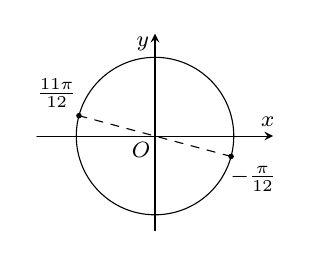
\begin{tikzpicture}[scale=1,>=stealth,font=\footnotesize,line join=round,line cap=round]
					\draw[->] (-1.5,0)--(1.5,0) node[shift={(110:.2)},scale=1]{$x$}; 
					\draw[->] (0,-1.2)--(0,1.3)  node[shift={(220:.2)},scale=1]{$y$};
					\path (0,0) coordinate (O)  node[shift={(-135:.25)},scale=1]{$O$};
					\draw (O)  circle (1cm);
					 \path
						 (-15:1) coordinate (M)
						 (165:1) coordinate (N);
					\draw[dashed](M)--(N); 
					\fill (M) node[shift={(-45:.4)}]{$-\frac{\pi}{12}$}circle  (1pt);
					\fill (N) node[shift={(135:.4)}]{$\frac{11\pi}{12}$}circle  (1pt);
				\end{tikzpicture}
		\end{center}
		Biểu diễn nghiệm  $x=\dfrac{\pi}{4}+k\pi$ trên đường tròn lượng giác ta được $2$ vị trí.
		\begin{center}
			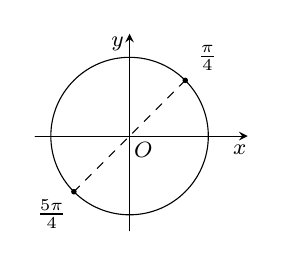
\begin{tikzpicture}[scale=1,>=stealth,font=\footnotesize,line join=round,line cap=round]
					\draw[->] (-1.2,0)--(1.5,0) node[shift={(-120:.2)},scale=1]{$x$}; 
					\draw[->] (0,-1.2)--(0,1.3) node[shift={(220:.2)},scale=1]{$y$}; 
					\path (0,0)  coordinate (O) node[shift={(-45:.25)},scale=1]{$O$};
					\draw  (O) circle (1cm);
					\path 
						 (45:1) coordinate (M)
						(-135:1) coordinate  (N);
					\draw[dashed](M)--(N); 
					\fill  (M) node[shift={(45:.4)}]{$\frac{\pi}{4}$}circle (1pt);
					\fill  (N) node[shift={(-135:.4)}]{$\frac{5\pi}{4}$}circle (1pt);
				\end{tikzpicture}
		\end{center}
		Vậy  có tất cả $4$ vị trí biểu diễn các nghiệm các nghiệm của phương trình.
	 }
\end{ex}

% nguồn: Ok_Toan11_TracNghiem_Lan2
\begin{ex}%[1D1H5-3]%[ma:da659577]
	Tính tổng các nghiệm thuộc khoảng $(0;\pi)$ của phương trình $\sin\left(2x-\dfrac{\pi}{4}\right)=\sin\left(x+\dfrac{3\pi}{4}\right)$. 
	 \choice
		{$\dfrac{7\pi}{2}$} 
		{\True $\pi$} 
		 {$\dfrac{3\pi}{2}$}
		 {$\dfrac{\pi}{4}$}
	\loigiai{ 
		 Ta có
		\allowdisplaybreaks 
		\begin{eqnarray*}
			 &&\sin\left(2x-\dfrac{\pi}{4}\right)=\sin\left(x+\dfrac{3\pi}{4}\right)\\
			&\Leftrightarrow& \hoac{ 
			&  2x-\dfrac{\pi}{4}=x+\dfrac{3\pi}{4}+k2\pi\\
			&  2x-\dfrac{\pi}{4}=\pi-x-\dfrac{3\pi}{4}+k2\pi
			 }\\
			&\Leftrightarrow& \hoac{ 
			& x=\pi+k2\pi\\ 
			&  x=\dfrac{\pi}{6}+k\dfrac{2\pi}{3}
			} (k\in\mathbb{Z}). 
		\end{eqnarray*}
		\begin{itemize}
			\item {\bfseries Trường hợp  1:} $x=\pi+k2\pi$ $(k\in\mathbb{Z})$.\\
			Do  $0<x<\pi$ nên $0<\pi+k2\pi <\pi$ $\Leftrightarrow$ $-\dfrac{1}{2}<k<0$. Vì $k\in\mathbb{Z}$ nên không có giá trị $k$.
			 \item {\bfseries Trường hợp 2:} $x=\dfrac{\pi}{6}+k\dfrac{2\pi}{3}$ $(k\in\mathbb{Z})$.\\
			Do $0<x<\pi$  nên $0<\dfrac{\pi}{6}+k\dfrac{2\pi}{3}<\pi$ $\Leftrightarrow$ $-\dfrac{1}{4}<k<\dfrac{5}{4}$. Vì $k\in\mathbb{Z}$ nên có hai giá trị $k$ là $k=0$; $k=1$.
			\begin{itemize}
				\item Với $k=0$, ta  được $x=\dfrac{\pi}{6}$.
				\item Với $k=1$,  ta được $x=\dfrac{5\pi}{6}$.
			\end{itemize}
			Do đó,  trên khoảng $(0;\pi)$ phương trình đã cho có hai nghiệm $x=\dfrac{\pi}{6}$ và $x=\dfrac{5\pi}{6}$.
		\end{itemize}
		Vậy tổng các nghiệm của phương  trình đã cho trong khoảng $(0;\pi)$ là $\dfrac{\pi}{6}+\dfrac{5\pi}{6}=\pi$.
	} 
\end{ex}

% nguồn: Ok_Toan11_TracNghiem_Lan2
\begin{ex}%[1D1H5-3]%[ma:8ec346a4]
	Nghiệm của  phương trình $\sin\dfrac{x}{2}=1$ là
	\choice 
		 {$x=\pi+k2\pi$}
		 {$x=k2\pi$}
		 {$x=\dfrac{\pi}{2}+k2\pi$}
		{\True $x=\pi+k4\pi$} 
	\loigiai{ 
		Ta có $\sin\dfrac{x}{2}=1\Leftrightarrow\dfrac{x}{2}=\dfrac{\pi}{2}+k2\pi\Leftrightarrow  x=\pi+k4\pi, k\in\mathbb{Z}$.\\
		Vậy phương trình  đã cho có nghiệm là $x=\pi+k4\pi, k\in\mathbb{Z}$.
	 }
\end{ex}

% nguồn: Ok_Toan11_TracNghiem_Lan2
\begin{ex}%[1D1H5-3]%[ma:b48d4423]
	Phương trình $\sin\left(3x+\dfrac{\pi}{3}\right)=-\dfrac{\sqrt{3}}{2}$ có bao nhiêu nghiệm thuộc  khoảng $\left(0;\dfrac{\pi}{2}\right)$?
	\choice 
		{$3$} 
		{$4$} 
		{$1$} 
		 {\True $2$}
	\loigiai{ 
		Ta có 
		\allowdisplaybreaks 
		\begin{eqnarray*}
			 &&\sin\left(3x+\dfrac{\pi}{3}\right)=-\dfrac{\sqrt{3}}{2}\\
			&\Leftrightarrow& \sin\left(3x+\dfrac{\pi}{3}\right)=\sin\left(-\dfrac{\pi}{3}\right)\\ 
			&\Leftrightarrow&  \hoac{
			& 3x+\dfrac{\pi}{3}=-\dfrac{\pi}{3}+k2\pi\\ 
			& 3x+\dfrac{\pi}{3}=\pi+\dfrac{\pi}{3}+k2\pi 
			}\\ 
			&\Leftrightarrow&  \hoac{
			& x=-\dfrac{2\pi}{9}+k\dfrac{2\pi}{3}\\ 
			&  x=\dfrac{\pi}{3}+k\dfrac{2\pi}{3}
			} (k\in\mathbb{Z}). 
		\end{eqnarray*}
		\begin{itemize}
			\item {\bfseries Trường hợp 1:} $x=-\dfrac{2\pi}{9}+k\dfrac{2\pi}{3}\in\left(0;\dfrac{\pi}{2}\right)$ $\Leftrightarrow$ $0<-\dfrac{2\pi}{9}+k\dfrac{2\pi}{3}<\dfrac{\pi}{2}$ $\Leftrightarrow$ $\dfrac{1}{3}<k<\dfrac{13}{12}$. Do $k\in\mathbb{Z}$ nên $k=1$. Suy ra trường hợp này có nghiệm  $x=\dfrac{4\pi}{9}$ thỏa mãn.
			\item {\bfseries Trường hợp 2:}  $x=\dfrac{\pi}{3}+k\dfrac{2\pi}{3}\in\left(0;\dfrac{\pi}{2}\right)$ $\Leftrightarrow$ $0<\dfrac{\pi}{3}+k\dfrac{2\pi}{3}<\dfrac{\pi}{2}$ $\Leftrightarrow$ $-\dfrac{1}{2}<k<\dfrac{1}{4}$. Do $k\in\mathbb{Z}$ nên $k=0$. Suy ra trường hợp này có nghiệm $x=\dfrac{\pi}{3}$ thỏa mãn.
		\end{itemize}
		 Vậy phương trình chỉ có $2$ nghiệm thuộc khoảng $\left(0;\dfrac{\pi}{2}\right)$.
	 }
\end{ex}

% nguồn: Ok_Toan11_TracNghiem_Lan2
\begin{ex}%[1D1H5-3]%[ma:f5ecc5f3]
	Nghiệm của phương trình $\sin  \dfrac{x}{2} = 1$ là
	 \choice
		{\True $x = \pi + k2\pi$, $k \in \mathbb{Z}$} 
		{$x = k2\pi$, $k  \in \mathbb{Z}$}
		{$x = -\pi + k2\pi$, $k \in  \mathbb{Z}$}
		{$x  = \dfrac{\pi}{2} + k2\pi$, $k \in \mathbb{Z}$}
	 \loigiai{
		Ta  có
		\begin{align*}
			\sin \dfrac{x}{2} = 1 \Leftrightarrow \dfrac{x}{2} =  \dfrac{\pi}{2} + k2\pi \Leftrightarrow x = \pi + k2\pi, k \in \mathbb{Z}.
		\end{align*}
		Vậy phương  trình có nghiệm là $x = \pi + k2\pi$, $k \in \mathbb{Z}.$
	 }
\end{ex}

% nguồn: Ok_Toan11_TracNghiem_Lan2
\begin{ex}%[1D1H5-3]%[ma:4a0de99a]
	Tập nghiệm của  phương trình $2\sin2x+1=0$ là
	\choice 
		 {\True $S=\left\{-\dfrac{\pi}{12}+k\pi;\dfrac{7\pi}{12}+k\pi\,\mid dle|\ k\in\mathbb{Z}\right\}$}
		{$S=\left\{-\dfrac{\pi}{6}+k2\pi;\dfrac{7\pi}{12}+k2\pi\,\mid  dle|\ k\in\mathbb{Z}\right\}$}
		{$S=\left\{-\dfrac{\pi}{12}+k2\pi;\dfrac{7\pi}{12}+k2\pi\,\mid dle|\  k\in\mathbb{Z}\right\}$}
		 {$S=\left\{-\dfrac{\pi}{6}+k\pi;\dfrac{7\pi}{12}+k\pi\,\mid dle|\ k\in\mathbb{Z}\right\}$}
	 \loigiai{
		 Ta có
		\allowdisplaybreaks 
		\begin{eqnarray*}
			&&2\sin2x+1=0\\ 
			 &\Leftrightarrow& \sin2x=-\dfrac{1}{2}\\
			&\Leftrightarrow&  \sin2x=\sin\left(-\dfrac{\pi}{6}\right)\\
			 &\Leftrightarrow& \hoac{
			&  2x=-\dfrac{\pi}{6}+k2\pi\\
			 & 2x=\dfrac{7\pi}{6}+k2\pi
			 }\\
			&\Leftrightarrow&  \hoac{
			&  x=-\dfrac{\pi}{12}+k\pi\\
			& x=\dfrac{7\pi}{12}+k\pi 
			 } (k\in\mathbb{Z}).
		\end{eqnarray*}
		 Vậy tập nghiệm của phương trình là $S=\left\{-\dfrac{\pi}{12}+k\pi;\dfrac{7\pi}{12}+k\pi\,\mid dle|\ k\in\mathbb{Z}\right\}$.
	} 
\end{ex}

% nguồn: Ok_Toan11_TracNghiem_Lan2
\begin{ex}%[1D1H5-3]%[ma:c7a004f8]
	 Tìm nghiệm của phương trình $\sin 2x = 1$.
	 \choice
		{$x = \dfrac{\pi}{2} + k2\pi$, $k \in  \mathbb{Z}$}
		{\True $x = \dfrac{\pi}{4} + k\pi$, $k \in  \mathbb{Z}$}
		 {$x = \dfrac{\pi}{4} + k2\pi$, $k \in \mathbb{Z}$}
		{$x = \dfrac{k\pi}{2}$,  $k \in \mathbb{Z}$}
	 \loigiai{
		Ta  có
		\begin{align*}
			\sin 2x = 1 \Leftrightarrow 2x = \dfrac{\pi}{2} + k2\pi  \Leftrightarrow x = \dfrac{\pi}{4} + k\pi, k \in \mathbb{Z}.
		\end{align*}
		Vậy phương trình có nghiệm là $x = \dfrac{\pi}{4} + k\pi$,  $k \in \mathbb{Z}$.
	} 
\end{ex}

% nguồn: Ok_Toan11_TracNghiem_Lan2
\begin{ex}%[1D1H5-3]%[ma:bf6da4c6]
	Hai góc lượng giác $\dfrac{\pi}{3}$ và $\dfrac{m\pi}{12}$ có cùng tia đầu và tia cuối khi $m$ có giá trị nào trong  các giá trị sau?
	\choice 
		{\True $m=4+24k$} 
		{$m=4+14k$} 
		 {$m=4+20k$}
		 {$m=4+22k$}
	 \loigiai{
		Để hai góc lượng giác trùng nhau thì tồn tại  một số nguyên $k$ sao cho
		$$\dfrac{m\pi}{12}-\dfrac{\pi}{3}=k2\pi \Leftrightarrow m-4=24k\Leftrightarrow m=4+24k,  (k\in \mathbb{Z})$$
	 }
\end{ex}

% nguồn: Ok_Toan11_TracNghiem_Lan2
\begin{ex}%[1D1H5-3]%[ma:937315db]
	Giải  phương trình $\sin\left(\pi-x\right)-\cos\left(\dfrac{\pi}{2}-2x\right)=0$.
	\choice 
		{$S=\left\{ k2\pi,k\in\mathbb{Z}\right\}$} 
		{\True $S=\left\{ k2\pi;\dfrac{\pi}{3}+\dfrac{k2\pi}{3},k\in\mathbb{Z}\right\}$} 
		 {$S=\left\{k\pi;\dfrac{\pi}{3}+\dfrac{k2\pi}{3},k\in\mathbb{Z}\right\}$}
		 {$S=\left\{\dfrac{\pi}{3}+\dfrac{k2\pi}{3},k\in\mathbb{Z}\right\}$}
	 \loigiai{
		Ta có 
		\begin{eqnarray*}
			\sin\left(\pi-x\right)-\cos\left(\dfrac{\pi}{2}-2x\right)=0&\Leftrightarrow&\sin x-\sin  2x=0\Leftrightarrow\sin 2x=\sin x\\ &\Leftrightarrow&\hoac{&2x=x+k2\pi\\& 2x=\pi-x+k2\pi}\Leftrightarrow\hoac{& x=k2\pi\\& x=\dfrac{\pi}{3}+\dfrac{k2\pi}{3}}\,(k\in\mathbb{Z}).
		\end{eqnarray*}
		Vậy tập nghiệm của phương trình đã cho là $S=\left\{k2\pi;\dfrac{\pi}{3}+\dfrac{k2\pi}{3}, k\in\mathbb{Z}\right\}$. 
	} 
\end{ex}

% nguồn: Ok_Toan11_TracNghiem_Lan2
\begin{ex}%[1D1H5-3]%[ma:17035c57]
	Phương trình  $\sin \left( \dfrac{2x}{3} - \dfrac{\pi}{3} \right) = 0$ có nghiệm là
	 \choice
		 {$x = \dfrac{\pi}{3} + k\pi$, $k \in \mathbb{Z}$}
		 {$x = k\pi$, $k \in \mathbb{Z}$}
		{$x = \dfrac{2\pi}{3} + \dfrac{k3\pi}{2}$, $k  \in \mathbb{Z}$}
		{\True $x  = \dfrac{\pi}{2} + \dfrac{k3\pi}{2}$, $k \in \mathbb{Z}$}
	\loigiai{ 
		Phương trình 
		\begin{align*}
			\sin \left( \dfrac{2x}{3} - \dfrac{\pi}{3} \right) = 0 \Leftrightarrow \dfrac{2x}{3} - \dfrac{\pi}{3} = k\pi \Leftrightarrow \dfrac{2x}{3} = \dfrac{\pi}{3} + k\pi \Leftrightarrow x  = \dfrac{\pi}{2} + \dfrac{k3\pi}{2}, k \in \mathbb{Z}.
		\end{align*}
		Vậy phương trình  có nghiệm là $x = \dfrac{\pi}{2} + \dfrac{k3\pi}{2}$, $k \in \mathbb{Z}.$
	 }
\end{ex}

% nguồn: Ok_Toan11_TracNghiem_Lan2
\begin{ex}%[1D1H5-3]%[ma:eb422dc9]
	Số nghiệm chung của hai phương trình $4\cos^2x-3=0$ và $2\sin x+1=0$ trên khoảng $\left(-\dfrac{\pi}{2};\dfrac{3\pi}{2}\right)$  bằng
	\choice 
		 {\True $2$}
		 {$4$}
		{$3$} 
		 {$1$}
	\loigiai{ 
		Trên khoảng $\left(-\dfrac{\pi}{2};\dfrac{3\pi}{2}\right)$ phương trình $2\sin x+1=0\Leftrightarrow\sin x=-\dfrac{1}{2}$ có hai nghiệm là $-\dfrac{\pi}{6}$  và $\dfrac{7\pi}{6}$.\\
		Cả hai nghiệm này đều  thỏa phương trình $4\cos^2x-3=0$.\\
	Vậy hai phương trình có  $2$ nghiệm chung.}
\end{ex}

% nguồn: Ok_Toan11_TracNghiem_Lan2
\begin{ex}%[1D1H5-3]%[ma:3259ffcf]
	Tập nghiệm của phương trình $\sin x = \sin \dfrac{5\pi}{3}$ là 
	 \choice
		{\True $\left\{ \dfrac{5\pi}{3} + k2\pi;  \dfrac{-2\pi}{3} + k2\pi \,\mid dle|\, k \in \mathbb{Z} \right\}$}
		{$\left\{ \dfrac{5\pi}{3} + k2\pi; \dfrac{7\pi}{3}  + k2\pi \,\mid dle|\, k \in \mathbb{Z} \right\}$}
		{$\left\{ \dfrac{5\pi}{3} + k2\pi; \dfrac{-5\pi}{3} + k2\pi \,\mid dle|\,  k \in \mathbb{Z} \right\}$}
		 {$\left\{ \dfrac{5\pi}{3} + k\pi; \dfrac{-2\pi}{3} + k\pi \,\mid dle|\, k \in \mathbb{Z} \right\}$}
	\loigiai{ 
		Áp dụng công thức nghiệm, ta có 
		\begin{align*}
			\sin x  = \sin \dfrac{5\pi}{3} \Leftrightarrow \hoac{
			&  x = \dfrac{5\pi}{3} + k2\pi \\
			& x =  \pi -\dfrac{5\pi}{3} + k2\pi} \Leftrightarrow \hoac{
			 & x = \dfrac{5\pi}{3} + k2\pi \\
			& x = -\dfrac{2\pi}{3} +  k2\pi}, k \in \mathbb{Z}.
		\end{align*}
		Vậy tập nghiệm của phương  trình là $\left\{ \dfrac{5\pi}{3} + k2\pi; \dfrac{-2\pi}{3} + k2\pi \,\mid dle|\, k \in \mathbb{Z} \right\}$.
	 }
\end{ex}

% nguồn: Ok_Toan11_TracNghiem_Lan2
\begin{ex}%[1D1H5-3]%[ma:759af294]
	Phương trình $2 \sin x-1=0$ có  bao nhiêu nghiệm $x \in(0;2\pi)$?
	\choice 
		 {\True $2$ nghiệm}
		{$1$ nghiệm} 
		 {$4$ nghiệm}
		{Vô  số nghiệm}
	 \loigiai{
		Ta có $2  \sin x-1=0
		\Leftrightarrow  \sin x=\dfrac{1}{2}
		\Leftrightarrow\hoac{&  x=\dfrac{\pi}{6}+2k\pi \\ & x=\dfrac{5\pi}{6}+2k\pi}(k \in \mathbb{Z})$.\\
		 Do $x \in(0;2\pi)$ nên ta có $x=\dfrac{\pi}{6}$; $x=\dfrac{5 \pi}{6}$.
	 }
\end{ex}

% nguồn: Ok_Toan11_TracNghiem_Lan2
\begin{ex}%[1D1H5-3]%[ma:ae3e7470]
	Tính tổng $S$ của  các nghiệm của phương trình $\sin x=\dfrac{1}{2}$ trên đoạn $\left[-\dfrac{\pi}{2};\dfrac{\pi}{2}\right]$.
	\choice 
		{$S=\dfrac{5\pi}{6}$} 
		 {$S=\dfrac{\pi}{3}$}
		{$S=\dfrac{\pi}{2}$} 
		{\True $S=\dfrac{\pi}{6}$} 
	\loigiai{ 
		Ta có  $\sin x=\dfrac{1}{2}$ $\Leftrightarrow$ $\hoac{
		&  x=\dfrac{\pi}{6}+2k\pi\\
		 & x=\dfrac{5\pi}{6}+2k\pi
		}$  $(k\in\mathbb{Z})$.
		\begin{itemize}
			 \item {\bfseries Trường hợp 1:} $x=\dfrac{\pi}{6}+k2\pi$ $(k\in\mathbb{Z})$.\\
			Vì $x\in\left[-\dfrac{\pi}{2};\dfrac{\pi}{2}\right]$ nên $-\dfrac{\pi}{2}\le \dfrac{\pi}{6}+k2\pi\le\dfrac{\pi}{2}$ $\Leftrightarrow$ $-\dfrac{1}{3}\le k\le \dfrac{1}{6}$. Hơn nữa,  $k\in\mathbb{Z}$ nên $k=0$. Khi đó, $x=\dfrac{\pi}{6}$.
			 \item {\bfseries Trường hợp 2:} $x=\dfrac{5\pi}{6}+k2\pi$ $(k\in\mathbb{Z})$.\\
			Vì $x\in\left[-\dfrac{\pi}{2};\dfrac{\pi}{2}\right]$ nên $-\dfrac{\pi}{2}\le \dfrac{5\pi}{6}+k2\pi\le\dfrac{\pi}{2}$ $\Leftrightarrow$  $-\dfrac{2}{3}\le k\le -\dfrac{1}{6}$. Trường hợp này không tồn tại $k\in\mathbb{Z}$.
		\end{itemize}
		Vậy  $S=\dfrac{\pi}{6}$.
	} 
\end{ex}

% nguồn: Ok_Toan11_TracNghiem_Lan2
\begin{ex}%[1D1H5-3]%[ma:549fe531]
	Tổng các nghiệm của phương trình $\tan 5x-\tan  x=0$ trên nửa khoảng $\left[0;\pi \right)$ bằng
	\choice 
		{$\dfrac{5\pi}{2}$} 
		{\True $\pi $} 
		 {$\dfrac{3\pi}{2}$}
		{$2\pi  $}
	\loigiai{Điều kiện xác định $\heva{&\cos 5x \neq 0\\& \cos x \neq 0 } \Leftrightarrow \heva{&x \neq \dfrac{\pi}{10}+k\dfrac{\pi}{5}\\&  x \neq \dfrac{\pi}{2}+k\pi } \Leftrightarrow x\neq \dfrac{\pi}{10}+k\dfrac{\pi}{5}$, $k\in\mathbb{Z}$. \\
		Ta có $\tan 5x-\tan  x=0\Leftrightarrow \tan 5x=\tan x\Leftrightarrow 5x=x+k\pi \Leftrightarrow x=\dfrac{k\pi}{4}$, $k\in\mathbb{Z}$.\\
		Kết hợp điều kiện ta có  nghiệm của phương trình là $\hoac{&x=k\pi \\ & x=\dfrac{\pi}{4}+k\pi \\& x=\dfrac{3\pi}{4}+k\pi}$, $k\in\mathbb{Z}$.\\
		 Vì $x\in \left[0;\pi \right)$, suy ra các nghiệm của phương trình trên $\left[0;\pi \right)$ là $\left\{0;\dfrac{\pi}{4};\dfrac{3\pi}{4} \right\}$.\\
	 Suy ra $0+\dfrac{\pi}{4}+\dfrac{3\pi}{4}=\pi$.}
\end{ex}

% nguồn: Ok_Toan11_TracNghiem_Lan2
\begin{ex}%[1D1H5-3]%[ma:5d314c37]
	 Số nghiệm của phương trình $\tan x=\tan \dfrac{3\pi}{11}$ trên khoảng $\left( \dfrac{\pi}{4};2\pi \right)$ là
	 \choice
		 {$4$}
		{$1$} 
		{\True $2$} 
		{$3$} 
	\loigiai{Ta có $\tan  x=\tan \dfrac{3\pi}{11}\Leftrightarrow x=\dfrac{3\pi}{11}+k\pi$, $k\in \mathbb{Z}$.\\
	Do $x\in \left( \dfrac{\pi}{4};2\pi \right)\Rightarrow \dfrac{\pi}{4}<\dfrac{3\pi}{11}+k\pi <2\pi \Rightarrow  k\in \left\{0;1 \right\}.$}
\end{ex}

% nguồn: Ok_Toan11_TracNghiem_Lan2
\begin{ex}%[1D1H5-3]%[ma:c9e00f06]
	Nghiệm của phương trình $\tan x-1=0$  là
	\choice 
		{$x=\dfrac{\pi}{6}+\dfrac{k\pi}{2}, k\in\mathbb{Z}$} 
		{$x=\dfrac{3\pi}{4}+k2\pi,  k\in\mathbb{Z}$}
		 {$x=\dfrac{-\pi}{4}+k\pi, k\in\mathbb{Z}$}
		{\True $x=\dfrac{\pi}{4}+k\pi, k\in\mathbb{Z}$} 
	\loigiai{ 
		Ta có $\tan x-1=0\Leftrightarrow\tan x=1\Leftrightarrow  x=\dfrac{\pi}{4}+k\pi, k\in\mathbb{Z}$.\\
		Vậy nghiệm của phương trình đã cho là $x=\dfrac{\pi}{4}+k\pi, k\in\mathbb{Z}$. 
	 }
\end{ex}

% nguồn: Ok_Toan11_TracNghiem_Lan2
\begin{ex}%[1D1H5-3]%[ma:882453b5]
	Số nghiệm của phương trình $\cos  x=\dfrac{1}{2}$ thuộc đoạn $[-2 \pi; 2 \pi]$ là
	 \choice
		{\True $4$} 
		{$2$} 
		{$3$} 
		 {$1$}
	\loigiai{ 
		 Ta có $\cos x=\dfrac{1}{2}\Leftrightarrow \hoac{&x=\dfrac{\pi}{3}+k 2 \pi, k \in \mathbb{Z} \\& x=-\dfrac{\pi}{3}+k 2 \pi, k \in \mathbb{Z}.}$
		\begin{itemize}
			\item Xét $x=\dfrac{\pi}{3}+k 2 \pi$, do $x \in[-2 \pi; 2 \pi]$ và $k \in  \mathbb{Z}$ nên $-2 \pi \leq \dfrac{\pi}{3}+k 2 \pi \leq 2 \pi \Rightarrow k=-1 $; $ k=0$.
			\item Xét $x=-\dfrac{\pi}{3}+k 2 \pi$, do $x \in[-2 \pi; 2 \pi]$ và $k \in  \mathbb{Z}$ nên $-2 \pi \leq-\dfrac{\pi}{3}+k 2 \pi \leq 2 \pi \Rightarrow k=1 $; $ k=0$.
		\end{itemize}
	Vậy phương trình có  $4$ nghiệm trên đoạn $[-2 \pi; 2 \pi]$.}
\end{ex}

% nguồn: Ok_Toan11_TracNghiem_Lan2
\begin{ex}%[1D1H5-3]%[ma:fadfacbb]
	Nghiệm của phương  trình $\sin x = \sin \dfrac{\pi}{5}$ là
	\choice 
		{$\hoac{& x = \dfrac{\pi}{5} + k\pi \\ & x = \dfrac{4\pi}{5} + k\pi}, k \in  \mathbb{Z}$}
		{\True $\hoac{& x = \dfrac{\pi}{5} + k2\pi \\ & x  = \dfrac{4\pi}{5} + k2\pi}, k \in \mathbb{Z}$}
		{$\hoac{&  x = \dfrac{\pi}{5} + k2\pi \\ & x = -\dfrac{\pi}{5} + k2\pi}, k \in \mathbb{Z}$}
		{$\hoac{& x = \dfrac{\pi}{5} +  k\pi \\ & x = -\dfrac{\pi}{5} + k\pi}, k \in \mathbb{Z}$}
	 \loigiai{
		 Ta có
		\begin{align*}
			\sin x = \sin \dfrac{\pi}{5} \Leftrightarrow  \hoac{
			&x  = \dfrac{\pi}{5} + k2\pi \\
			&x = \pi -\dfrac{\pi}{5} +  k2\pi} \Leftrightarrow \hoac{
			&x = \dfrac{\pi}{5} + k2\pi  \\
			&x = \dfrac{4\pi}{5} +  k2\pi}, k \in \mathbb{Z}.
		\end{align*}
		Vậy nghiệm của phương trình là $x = \dfrac{\pi}{5} + k2\pi$ và $x = \dfrac{4\pi}{5}  + k2\pi$, $k \in \mathbb{Z}$.
	 }
\end{ex}

% nguồn: Ok_Toan11_TracNghiem_Lan2
\begin{ex}%[1D1H5-3]%[ma:a57641d2]
	Phương trình $\tan  x+1=0$ có nghiệm là
	 \choice
		{$x=\dfrac{\pi}{4}+k\pi$, $k\in\mathbb{Z}$} 
		 {$x=-\dfrac{\pi}{2}+k\pi$, $k\in\mathbb{Z}$}
		 {\True $x=-\dfrac{\pi}{4}+k\pi$, $k\in\mathbb{Z}$}
		{$x=\dfrac{\pi}{4}+k\pi$,  $x=-\dfrac{\pi}{4}+k\pi$, $k\in\mathbb{Z}$}
	 \loigiai{
	Ta có  $\tan x+1=0\Leftrightarrow \tan x=-1\Leftrightarrow \tan x=\tan \left( -\dfrac{\pi}{4} \right)\Leftrightarrow x=-\dfrac{\pi}{4}+k\pi, k\in\mathbb{Z}$.}
\end{ex}

% nguồn: Ok_Toan11_TracNghiem_Lan2
\begin{ex}%[1D1H5-3]%[ma:08ecfd1e]
	Số nghiệm của phương trình $\sin\left(x+\dfrac{\pi}{4}\right)=1$ (với $\pi\le x\le 5\pi$) là 
	 \choice
		{$1$} 
		{$0$} 
		 {$2$}
		 {\True $3$}
	 \loigiai{
		Ta có $\sin\left(x+\dfrac{\pi}{4}\right)=1$  $\Leftrightarrow x+\dfrac{\pi}{4}=\dfrac{\pi}{2}+k2\pi$ $\Leftrightarrow x=\dfrac{\pi}{4}+k2\pi$, $k\in\mathbb{Z}$.\\
		Ta  có $\pi\le x\le 5\pi\Leftrightarrow\pi\le\dfrac{\pi}{4}+k2\pi\le 5\pi\Leftrightarrow\dfrac{3}{8}\le k\le\dfrac{19}{8}$.\\
		Vì $k\in\mathbb{Z}$ nên  $k\in\left\{1;2;3\right\}$.\\
		Vậy phương trình $\sin\left(x+\dfrac{\pi}{4}\right)=1$ có $3$ nghiệm thỏa  mãn $\pi\le x\le 5\pi$.
	} 
\end{ex}

% nguồn: Ok_Toan11_TracNghiem_Lan2
\begin{ex}%[1D1H5-3]%[ma:b08b050f]
	Số nghiệm  thuộc khoảng $(0;2\pi)$ của phương trình $\sin\left(x+\dfrac{\pi}{3}\right)+\sin 2x=0$ là
	\choice 
		 {$1$}
		 {$2$}
		 {$3$}
		 {\True $4$}
	\loigiai{ 
		Ta có 
		 \allowdisplaybreaks
		\begin{eqnarray*}
			 &&\sin\left(x+\dfrac{\pi}{3}\right)+\sin 2x=0\\
			 &\Leftrightarrow&\sin\left(x+\dfrac{\pi}{3}\right)=-\sin 2x\\
			&\Leftrightarrow&\sin\left(x+\dfrac{\pi}{3}\right)=\sin(-2x)\\ 
			&\Leftrightarrow&\hoac{ 
			& x+\dfrac{\pi}{3}=-2x+k2\pi\\ 
			 & x+\dfrac{\pi}{3}=\pi+2x+k2\pi
			 }\\
			 &\Leftrightarrow&\hoac{
			&  x=-\dfrac{\pi}{9}+k\dfrac{2\pi}{3}\\
			&  x=-\dfrac{2\pi}{3}-k2\pi
			} (k\in\mathbb{Z}). 
		\end{eqnarray*}
		\begin{itemize}
			\item {\bfseries Trường hợp 1:} $x=-\dfrac{\pi}{9}+k\dfrac{2\pi}{3}\in(0;2\pi)$ $\Leftrightarrow$ $0<-\dfrac{\pi}{9}+k\dfrac{2\pi}{3}<2\pi$ $\Leftrightarrow$ $\dfrac{1}{6}<k<\dfrac{19}{6}$. Hơn nữa, $k\in\mathbb{Z}$ nên $k=1$ hoặc $k=2$ hoặc $k=3$.  Khi đó, $x=\dfrac{5\pi}{9}$ hoặc $x=\dfrac{11\pi}{9}$ hoặc $x=\dfrac{17\pi}{9}$.
			\item {\bfseries Trường hợp 2:} $x=-\dfrac{2\pi}{3}-k2\pi\in(0;2\pi)$ $\Leftrightarrow$ $0<-\dfrac{2\pi}{3}-k2\pi<2\pi$ $\Leftrightarrow$ $-\dfrac{4}{3}<k<-\dfrac{1}{3}$. Hơn nữa, $k\in\mathbb{Z}$ nên $k=-1$. Khi đó, $x=\dfrac{4\pi}{3}$. 
		\end{itemize}
		Vậy có $4$  nghiệm thỏa mãn yêu cầu bài toán.
	 }
\end{ex}

% nguồn: Ok_Toan11_TracNghiem_Lan2
\begin{ex}%[1D1H5-3]%[ma:e1aa6f26]
	Phương trình $\sin x = \dfrac{\sqrt{3}}{2}$ có nghiệm là 
	\choice 
		{\True $\hoac{&x  = \dfrac{\pi}{3} + k2\pi \\ &x =\dfrac{2\pi}{3}+k2\pi}, k \in \mathbb{Z}$}
		{$\hoac{&x =  -\dfrac{\pi}{3} + k2\pi \\ &x =\dfrac{4\pi}{3}+k2\pi}, k \in \mathbb{Z}$}
		{$\hoac{&x  = \dfrac{\pi}{4} + k2\pi \\ &x =\dfrac{3\pi}{4}+k2\pi}, k \in \mathbb{Z}$}
		{$\hoac{&x = \dfrac{\pi}{3} + k2\pi \\ &x =-\dfrac{2\pi}{3}+k2\pi}, k \in \mathbb{Z}$} 
	 \loigiai{
		Ta  có
		\begin{align*}
			\sin x = \dfrac{\sqrt{3}}{2}  \Leftrightarrow \sin x = \sin \dfrac{\pi}{3} \Leftrightarrow \hoac{
			& x =  \dfrac{\pi}{3} + k2\pi \\
			&  x =\pi - \dfrac{\pi}{3} + k2\pi} \Leftrightarrow \hoac{
			 & x = \dfrac{\pi}{3} + k2\pi \\
			& x = \dfrac{2\pi}{3} +  k2\pi}, k \in \mathbb{Z}.
		\end{align*}
		Vậy phương trình có nghiệm là $x  = \dfrac{\pi}{3} + k2\pi$; $x =\dfrac{2\pi}{3}+k2\pi$, $k \in \mathbb{Z}$.
	} 
\end{ex}

% nguồn: Ok_Toan11_TracNghiem_Lan2
\begin{ex}%[1D1H5-3]%[ma:a11f774d]
	Tập nghiệm của phương trình $2\sin\dfrac{x}{2}-1=0$  là
	 \choice
		{$S=\left\lbrace\dfrac{\pi}{6}+k2\pi;\dfrac{5\pi}{6}+k2\pi\mid k\in\mathbb{Z}\right\rbrace$} 
		{\True  $S=\left\lbrace\dfrac{\pi}{3}+k4\pi;\dfrac{5\pi}{3}+k4\pi\mid k\in\mathbb{Z}\right\rbrace$}
		 {$S=\left\lbrace-\dfrac{\pi}{3}+k4\pi;\dfrac{\pi}{3}+k4\pi\mid k\in\mathbb{Z}\right\rbrace$}
		{$S=\left\lbrace\dfrac{\pi}{3}+k2\pi;\dfrac{5\pi}{3}+k2\pi\mid k\in\mathbb{Z}\right\rbrace$} 
	 \loigiai{
		Ta  có $2\sin\dfrac{x}{2}-1=0
		 \Leftrightarrow\sin\dfrac{x}{2}=\dfrac{1}{2}
		\Leftrightarrow 
		 \hoac{&\dfrac{x}{2}=\dfrac{\pi}{6}+k2\pi\\
		&\dfrac{x}{2}=\pi-\dfrac{\pi}{6}+k2\pi}  (k\in\mathbb{Z})
		\Leftrightarrow\hoac{&x=\dfrac{\pi}{3}+k4\pi\\ 
		&x=\dfrac{5\pi}{3}+k4\pi}  (k\in\mathbb{Z})$.\\
		Vậy phương trình  đã cho có tập nghiệm là $S=\left\lbrace\dfrac{\pi}{3}+k4\pi;\dfrac{5\pi}{3}+k4\pi\mid k\in\mathbb{Z}\right\rbrace$.
	} 
\end{ex}

% nguồn: Ok_Toan11_TracNghiem_Lan2
\begin{ex}%[1D1H5-3]%[ma:137536d7]
	Nghiệm của phương  trình $2\sin x+1=0$ là
	\choice 
		{$x=\dfrac{\pi}{6}+k2\pi$;  $x=\dfrac{7\pi}{6}+k2\pi$}
		 {\True $x=-\dfrac{\pi}{6}+k2\pi$; $x=\dfrac{7\pi}{6}+k2\pi$}
		{$x=\pi+k2\pi$; $x=\dfrac{\pi}{8}+k2\pi$} 
		 {$x=-\dfrac{\pi}{6}+k2\pi$; $x=\dfrac{5\pi}{6}+k2\pi$}
	\loigiai{ 
		 Ta có $2\sin x+1=0
		\Leftrightarrow\sin  x=\dfrac{-1}{2}
		 \Leftrightarrow
		 \hoac{&x=-\dfrac{\pi}{6}+k2\pi\\
		 &x=\pi+\dfrac{\pi}{6}+k2\pi}
		\Leftrightarrow 
		 \hoac{&x=-\dfrac{\pi}{6}+k2\pi\\
		&x=\dfrac{7\pi}{6}+k2\pi} 
		(k\in\mathbb{Z})$.\\ 
		Vậy phương trình đã cho có các nghiệm là $x=-\dfrac{\pi}{6}+k2\pi, k\in\mathbb{Z}$  và $x=\dfrac{7\pi}{6}+k2\pi, k\in\mathbb{Z}$.
	 }
\end{ex}

% nguồn: Ok_Toan11_TracNghiem_Lan2
\begin{ex}%[1D1H5-3]%[ma:96810afb]
	Cho hai phương trình $\cos 3 x-1=0  $\qquad (1); $ \cos 2 x=-\dfrac{1}{2}$\qquad (2). Tập các nghiệm của phương trình $(1)$ đồng thời là nghiệm của phương trình $(2)$ là
	 \choice
		{$x=\dfrac{\pi}{3}+k 2  \pi$, $ k \in \mathbb{Z}$}
		{$x=k 2 \pi$,  $ k \in \mathbb{Z}$}
		{$x= \pm \dfrac{\pi}{3}+k 2 \pi$, $ k  \in \mathbb{Z}$}
		{\True $x= \pm \dfrac{2 \pi}{3}+k 2 \pi$, $  k \in \mathbb{Z}$}
	 \loigiai{
		 Ta có
		\begin{itemize}
			\item $\cos 3  x-1=0 \Leftrightarrow \cos 3 x=1 \Leftrightarrow x=k \dfrac{2 \pi}{3}, k \in \mathbb{Z}$.
			\item $\cos 2 x=-\dfrac{1}{2}\Leftrightarrow 2 x=  \pm \dfrac{2 \pi}{3}+k 2 \pi \Leftrightarrow x= \pm \dfrac{\pi}{3}+k \pi, k \in \mathbb{Z}$.
		\end{itemize}
	Biểu diễn các nghiệm trên đường tròn lượng giác ta có tập các  nghiệm của phương trình $(1)$ đồng thời là nghiệm của phương trình $(2)$ là $x= \pm \dfrac{2 \pi}{3}+k \pi$, $ k \in \mathbb{Z}$.}
\end{ex}

% nguồn: Ok_Toan11_TracNghiem_Lan2
\begin{ex}%[1D1H5-3]%[ma:2ff4f321]
	Tính tổng các nghiệm trong đoạn $\left[0;30 \right]$ của phương trình $\tan  x=\tan 3x$.
	\choice 
		 {$55\pi$}
		{$\dfrac{171\pi}{2}$} 
		{\True $45\pi$} 
		{$\dfrac{190\pi}{2}$} 
	\loigiai{Điều kiện để phương trình có nghĩa $\heva{&\cos x\ne 0 \\&\cos 3x\ne 0}\Leftrightarrow \heva{ &  x\ne \dfrac{\pi}{2}+k\pi \\ & x\ne \dfrac{\pi}{6}+\dfrac{k\pi}{3}}$, $k\in\mathbb{Z}$.\\
		Khi đó, phương  trình đã cho tương đương với $3x=x+k\pi \Leftrightarrow x=\dfrac{k\pi}{2}$, $k\in\mathbb{Z}$.\\
		So sánh với điều kiện ta được $\hoac{&x=k2\pi \\&x=\pi +k2\pi}$,  $k\in\mathbb{Z}$.\\
		 Ta có ngay $x\in \left[0;30 \right]\Rightarrow k\in \left\{0;...;4 \right\}\Rightarrow x\in \left\{0;\pi;2\pi;....;9\pi \right\}$.\\
	Vậy tổng  các nghiệm trong đoạn $\left[0;30 \right]$ của phương trình là $45\pi$.}
\end{ex}

% nguồn: Ok_Toan11_TracNghiem_Lan2
\begin{ex}%[1D1H5-3]%[ma:be32eedf]
	Giải phương trình $\cot\left( 3x-1 \right)=-\sqrt{3}$. 
	\choice 
		{\True $x=\dfrac{1}{3}+\dfrac{5\pi}{18}+k\dfrac{\pi}{3}$, $k\in  \mathbb{Z}$}
		 {$x=\dfrac{1}{3}+\dfrac{\pi}{18}+k\dfrac{\pi}{3}$, $k\in \mathbb{Z}$}
		{$x=\dfrac{5\pi}{18}+k\dfrac{\pi}{3}$, $k\in \mathbb{Z}$} 
		{$x=\dfrac{1}{3}-\dfrac{\pi}{6}+k\pi $, $k\in  \mathbb{Z}$}
	\loigiai{Ta có $\cot\left( 3x-1 \right)=-\sqrt{3}\Leftrightarrow \cot\left( 3x-1  \right)=\cot\left( -\dfrac{\pi}{6} \right)$\\
		$\Leftrightarrow  3x-1=\dfrac{-\pi}{6}+k\pi \Leftrightarrow x=\dfrac{1}{3}-\dfrac{\pi}{18}+k\dfrac{\pi}{3}$, $k\in\mathbb{Z}$.\\
	Với $k=1$ thì $x=\dfrac{1}{3}+\dfrac{5\pi}{18}$,  do đó $x=\dfrac{1}{3}+\dfrac{5\pi}{18}+k\dfrac{\pi}{3}$.}
\end{ex}

% nguồn: Ok_Toan11_TracNghiem_Lan2
\begin{ex}%[1D1H5-3]%[ma:72d7e94c]
	Phương trình  $\cot 3x=\cot x$ có các nghiệm là
	 \choice
		{$x=\dfrac{\pi}{2}+k2\pi $, $k\in\mathbb{Z}$} 
		{$x=k\pi  $, $k\in\mathbb{Z}$}
		{$x=\dfrac{k\pi}{3}$, $k\in\mathbb{Z}$} 
		{\True $x=\dfrac{\pi}{2}+k\pi  $, $k\in\mathbb{Z}$}
	\loigiai{ĐKXĐ: $\heva{& \sin 3x\ne 0 \\ &\sin x\ne 0  } \Leftrightarrow \heva{& x\ne k\dfrac{\pi}{3} \\ & x\ne k\pi}$, $k\in\mathbb{Z}$.\\
		Phương trình tương  đương
		\begin{eqnarray*}
			&& \dfrac{\cos 3x}{\sin 3x}=\dfrac{\cos  x}{\sin x}\\
			&\Leftrightarrow& \sin x\cos  3x-\cos x\sin 3x=0 \\
			&\Leftrightarrow&  \sin 2x=0 \\
			 &\Leftrightarrow& x=k\dfrac{\pi}{2}, k\in\mathbb{Z}
		\end{eqnarray*}
	Kết  hợp điều kiện ta được các nghiệm của phương trình $x=\dfrac{\pi}{2}+k\pi$, $k\in\mathbb{Z}$.}
\end{ex}

% nguồn: Ok_Toan11_TracNghiem_Lan2
\begin{ex}%[1D1H5-3]%[ma:c0ebf14a]
	Nghiệm của phương trình  $\tan 2x=\tan\left(\dfrac{\pi}{2}-x\right)$ là
	\choice 
		 {$x=\dfrac{\pi}{6}+\dfrac{k\pi}{2}, k\in\mathbb{Z}$}
		{$x=\dfrac{\pi}{4}+\dfrac{k\pi}{3}, k\in\mathbb{Z}$} 
		{$x=\dfrac{\pi}{3}+\dfrac{k\pi}{2},  k\in\mathbb{Z}$}
		{\True  $x=\dfrac{\pi}{6}+\dfrac{k\pi}{3}, k\in\mathbb{Z}$}
	\loigiai{ 
		 Ta có $\tan 2x=\tan\left(\dfrac{\pi}{2}-x\right)\Leftrightarrow 2x=\dfrac{\pi}{2}-x+k\pi\Leftrightarrow x=\dfrac{\pi}{6}+\dfrac{k\pi}{3}, k\in\mathbb{Z}$.\\
		Vậy phương trình  đã cho có nghiệm là $x=\dfrac{\pi}{6}+\dfrac{k\pi}{3}, k\in\mathbb{Z}$.
	} 
\end{ex}

% nguồn: Ok_Toan11_TracNghiem_Lan2
\begin{ex}%[1D1H5-3]%[ma:822c0a17]
	Giải phương trình  $\cot \dfrac{2x}{3}=\sqrt{3}$.
	 \choice
		{$x=\dfrac{\pi}{4}+k\pi $, $k\in \mathbb{Z}$} 
		{$x=\dfrac{\pi}{4}+\dfrac{2k\pi}{3}  $, $k\in \mathbb{Z}$}
		{\True  $x=\dfrac{\pi}{4}+\dfrac{k3\pi}{2} $, $k\in \mathbb{Z}$}
		{$x=\dfrac{\pi}{2}+\dfrac{3k\pi}{2}  $, $k\in \mathbb{Z}$}
	\loigiai{Ta có $\cot \dfrac{2x}{3}=\sqrt{3}\Leftrightarrow \cot \dfrac{2x}{3}=\cot \dfrac{\pi}{6}\Leftrightarrow \dfrac{2x}{3}=\dfrac{\pi}{6}+k\pi \Leftrightarrow x=\dfrac{\pi}{4}+\dfrac{k3\pi}{2} $, $k\in \mathbb{Z}$.} 
\end{ex}

% nguồn: Ok_Toan11_TracNghiem_Lan2
\begin{ex}%[1D1H5-3]%[ma:8b3c238d]
	Tập nghiệm của phương trình $\cot x=\sqrt{3}$  là
	\choice 
		{\True $\left\{\dfrac{-5\pi}{6}+k\pi; k\in  \mathbb{Z} \right\}$}
		{$\left\{\pm \dfrac{\pi}{6}+k\pi; k\in \mathbb{Z} \right\}$} 
		{$\left\{\dfrac{\pi}{3}+k\pi; k\in \mathbb{Z}  \right\}$}
		{$\left\{\dfrac{\pi}{6}+k2\pi;  k\in \mathbb{Z} \right\}$}
	\loigiai{Ta  có $\cot x=\sqrt{3}\Leftrightarrow \cot x=\cot \dfrac{\pi}{6}\Leftrightarrow x=\dfrac{\pi}{6}+k\pi$, $k\in\mathbb{Z}\Leftrightarrow x=\dfrac{-5\pi}{6}+k\pi$, $k\in\mathbb{Z}$.}
\end{ex}

% nguồn: Ok_Toan11_TracNghiem_Lan2
\begin{ex}%[1D1H5-3]%[ma:886e210d]
	Số nghiệm thực  của phương trình $2\sin x-1=0$ trên đoạn $\left[-\dfrac{3\pi}{2};10\pi\right]$ là
	 \choice
		{\True  $11$}
		{$9$} 
		{$20$} 
		{$21$} 
	 \loigiai{
		Ta có $2\sin x-1=0$ $\Leftrightarrow$ $\sin x=\dfrac{1}{2}$  $\Leftrightarrow\hoac{
		&  x=\dfrac{\pi}{6}+k2\pi\\
		& x=\dfrac{5\pi}{6}+k2\pi 
		}$ $(k\in\mathbb{Z})$. 
		\begin{itemize}
			\item {\bfseries Trường hợp 1:} $x=\dfrac{\pi}{6}+k2\pi$, ta có $-\dfrac{3\pi}{2}\le\dfrac{\pi}{6}+k2\pi\le 10\pi$ $\Leftrightarrow-\dfrac{5}{6}\le k\le\dfrac{59}{12}$. Vì $k\in\mathbb{Z}$ nên $0\le k\le 4$, $k\in\mathbb{Z}$. Do đó, trường hợp này phương trình  có $5$ nghiệm.
			\item {\bfseries Trường hợp 2:} $x=\dfrac{5\pi}{6}+k2\pi$ ta có  $-\dfrac{3\pi}{2}\le\dfrac{5\pi}{6}+k2\pi\le 10\pi$ $\Leftrightarrow-\dfrac{7}{6}\le k\le\dfrac{55}{12}$. Vì $k\in\mathbb{Z}$ nên $-1\le k\le 4$, $k\in\mathbb{Z}$. Do đó, trường hợp này phương trình có $6$ nghiệm.
		\end{itemize}
		 Rõ ràng các nghiệm này khác nhau từng đôi một, vì $\dfrac{\pi}{6}+k2\pi=\dfrac{5\pi}{6}+k'2\pi\Leftrightarrow k-k'=\dfrac{1}{3}$ (vô lý).\\
		Vậy phương trình có $11$ nghiệm trên  đoạn $\left[-\dfrac{3\pi}{2};10\pi\right]$.
	 }
\end{ex}

% nguồn: Ok_Toan11_TracNghiem_Lan2
\begin{ex}%[1D1H5-3]%[ma:ed2c9ae4]
	Tập nghiệm  của phương trình $2\sin 2x=\sqrt{2}$ là
	\choice 
		{$S=\left\lbrace\dfrac{\pi}{4}+k2\pi;\dfrac{3\pi}{4}+k2\pi\mid  k\in\mathbb{Z}\right\rbrace$}
		{\True $S=\left\lbrace\dfrac{\pi}{8}+k\pi;\dfrac{3\pi}{8}+k\pi\mid k\in\mathbb{Z}\right\rbrace$} 
		 {$S=\left\lbrace\dfrac{\pi}{8}+k2\pi;\dfrac{3\pi}{8}+k2\pi\mid k\in\mathbb{Z}\right\rbrace$}
		{$S=\left\lbrace\dfrac{\pi}{4}+k\pi;\dfrac{3\pi}{4}+k\pi\mid k\in\mathbb{Z}\right\rbrace$} 
	\loigiai{ 
		 Ta có
		\[ 
		 2\sin 2x=\sqrt{2}\Leftrightarrow\sin 2x=\dfrac{\sqrt{2}}{2}
		\Leftrightarrow\sin  2x=\sin\dfrac{\pi}{4}
		\Leftrightarrow\hoac{&2x=\dfrac{\pi}{4}+k2\pi\\ 
		 &2x=\dfrac{3\pi}{4}+k2\pi}
		 \Leftrightarrow\hoac{&x=\dfrac{\pi}{8}+k\pi\\
		 &x=\dfrac{3\pi}{8}+k\pi} (k\in\mathbb{Z}).
		 \]
		Vậy tập nghiệm của phương trình đã cho là  $S=\left\lbrace\dfrac{\pi}{8}+k\pi;\dfrac{3\pi}{8}+k\pi\mid k\in\mathbb{Z}\right\rbrace$.
	 }
\end{ex}

% nguồn: Ok_Toan11_TracNghiem_Lan2
\begin{ex}%[1D1H5-3]%[ma:d7b93f34]
	Tập nghiệm $S$ của phương trình $\sqrt{3}\tan\dfrac{x}{3}+3=0$. 
	 \choice
		 {$S=\left\lbrace-\dfrac{\pi}{9}+k3\pi\mid k\in\mathbb{Z}\right\rbrace$}
		 {$S=\left\lbrace-\dfrac{\pi}{3}+k\pi\mid k\in\mathbb{Z}\right\rbrace$}
		 {\True $S=\left\lbrace-\pi+k3\pi\mid k\in\mathbb{Z}\right\rbrace$}
		{$S=\left\lbrace\dfrac{\pi}{6}+k\pi\mid k\in\mathbb{Z}\right\rbrace$} 
	 \loigiai{
		Ta có $\sqrt{3}\tan\dfrac{x}{3}+3=0\Leftrightarrow\tan\dfrac{x}{3}=-\sqrt{3}=\tan\left(-\dfrac{\pi}{3}\right)\Leftrightarrow\dfrac{x}{3}=-\dfrac{\pi}{3}+k\pi\Leftrightarrow x=-\pi+k3\pi, k\in \mathbb{Z}$.\\ 
		Vậy  phương trình đã cho có tập nghiệm là $S=\left\lbrace-\pi+k3\pi\mid k\in\mathbb{Z}\right\rbrace$.
	} 
\end{ex}

% nguồn: Ok_Toan11_TracNghiem_Lan2
\begin{ex}%[1D1H5-3]%[ma:684d4d17]
	Nghiệm của phương  trình $\cos x=\dfrac{\sqrt{3}}{2}$ là
	\choice 
		{$x= \pm  \dfrac{\sqrt{3}}{2}+k2\pi$ $\,(k \in \mathbb{Z})$}
		{$x= \pm \dfrac{\pi}{6}+k  \pi$ $\,(k \in \mathbb{Z})$}
		{\True $x= \pm \dfrac{\pi}{6}+k2\pi$ $\,(k  \in \mathbb{Z})$}
		 {$x= \pm \dfrac{\pi}{3}+k2\pi$ $\,(k \in \mathbb{Z})$}
	 \loigiai{
		Ta có $\cos x=\dfrac{\sqrt{3}}{2} \Leftrightarrow \cos x=\cos \dfrac{\pi}{6} \Leftrightarrow x= \pm \dfrac{\pi}{6}+k 2 \pi$ $\,(k \in \mathbb{Z})$. 
	} 
\end{ex}

% nguồn: Ok_Toan11_TracNghiem_Lan2
\begin{ex}%[1D1H5-3]%[ma:78712acf]
	Trong khoảng $\left(0;\pi \right)$, phương trình $\cos 4x+\sin  x=0$ có tập nghiệm là $S$. Hãy xác định $S$.
	 \choice
		{$S=\left\{\dfrac{\pi}{3};\dfrac{2\pi}{3};\dfrac{3\pi}{10};\dfrac{7\pi}{10} \right\}$} 
		 {$S=\left\{\dfrac{\pi}{6};\dfrac{3\pi}{10} \right\}$}
		{$S=\left\{\dfrac{\pi}{6};\dfrac{\pi}{10};\dfrac{7\pi}{10} \right\}$} 
		 {\True $S=\left\{\dfrac{\pi}{6};\dfrac{5\pi}{6};\dfrac{3\pi}{10};\dfrac{7\pi}{10} \right\}$}
	\loigiai{ 
		 Ta có
		\begin{eqnarray*}
			& &\cos 4x+\sin  x=0\\
			&\Leftrightarrow&  \cos4x=-\sin x\\
			&\Leftrightarrow& \cos4x=\sin \left(-x\right)\\ 
			&\Leftrightarrow&  \cos4x=\cos\left(\dfrac{\pi}{2}+x\right)\\
			 &\Leftrightarrow& \hoac{&{4x=\dfrac{\pi}{2}+x+k2\pi} \\
			 &{4x=-\dfrac{\pi}{2}-x+k2\pi}
			 } \Leftrightarrow \hoac{&{x=\dfrac{\pi}{6}+k\dfrac{2\pi}{3}} \\
			 &{x=-\dfrac{\pi}{10}+k\dfrac{2\pi}{5}}
			},\, k\in \mathbb{Z}. 
		\end{eqnarray*}
		Vì $x\in \left(0;\pi \right)$ nên $S=\left\{\dfrac{\pi}{6};\dfrac{5\pi}{6};\dfrac{3\pi}{10};\dfrac{7\pi}{10}  \right\}$.
	} 
\end{ex}

% nguồn: Ok_Toan11_TracNghiem_Lan2
\begin{ex}%[1D1H5-3]%[ma:1ac898e5]
	Giải phương trình  $\sqrt{3}\tan x-1=0$.
	\choice 
		 {$x=\dfrac{\pi}{3}+k\pi, k\in\mathbb{Z}$}
		{$x=\dfrac{\pi}{6}+\dfrac{k\pi}{2}, k\in\mathbb{Z}$} 
		{\True $x=\dfrac{\pi}{6}+k\pi, k\in\mathbb{Z}$} 
		 {$x=-\dfrac{\pi}{6}+k\pi, k\in\mathbb{Z}$}
	 \loigiai{
		Điều kiện $x\neq\dfrac{\pi}{2}+k\pi, k\in\mathbb{Z}$.  Ta có
		\begin{eqnarray*}
			\sqrt{3}\tan  x-1=0\Leftrightarrow\tan x=\dfrac{1}{\sqrt{3}}
			\Leftrightarrow\tan x=\tan\dfrac{\pi}{6}\Leftrightarrow x=\dfrac{\pi}{6}+k\pi,  k\in\mathbb{Z}.
		\end{eqnarray*}
		Vậy  phương trình đã cho có nghiệm là $x=\dfrac{\pi}{6}+k\pi, k\in\mathbb{Z}$.
	 }
\end{ex}

% nguồn: Ok_Toan11_TracNghiem_Lan2
\begin{ex}%[1D1H5-3]%[ma:fe0eca91]
	Số nghiệm của phương trình $\cot 20x=1$ trên đoạn $\left[-50\pi;0 \right]$  là
	\choice 
		 {$980$}
		 {$1\,001$}
		{\True  $1\,000$}
		{$981$} 
	\loigiai{Ta có  $\cot 20x=1\Leftrightarrow 20x=\dfrac{\pi}{4}+k\pi \Leftrightarrow x=\dfrac{\pi}{80}+k\dfrac{\pi}{20}$, $k\in\mathbb{Z}$. \\
		Theo giả thiết $-50\pi \le  x\le 0$, với $x=\dfrac{\pi}{80}+k\dfrac{\pi}{20}$ ta có
		\begin{eqnarray*}
			&& -50\pi  \le \dfrac{\pi}{80}+k\dfrac{\pi}{20}\le 0 \\
			&\Leftrightarrow& -50\pi -\dfrac{\pi}{80}\le  k\dfrac{\pi}{20}\le -\dfrac{\pi}{80} \\
			&\Leftrightarrow& -1\,000-\dfrac{1}{4}\le k\le  -\dfrac{1}{4}, k\in\mathbb{Z}.
		\end{eqnarray*}
		Do đó $k\in \left\{-1\,000,-999,...,-1 \right\}$. \\ 
	Vậy phương  trình đã cho có $1\,000$ nghiệm trên $\left[-50\pi;0 \right].$}
\end{ex}

% nguồn: Ok_Toan11_TracNghiem_Lan2
\begin{ex}%[1D1H5-3]%[ma:37747ff8]
	Tìm  nghiệm của phương trình $\sin \left( x + \dfrac{\pi}{6} \right) = 1$.
	\choice 
		 {\True $x = \dfrac{\pi}{3} + k2\pi$, $k \in \mathbb{Z}$}
		{$x = -\dfrac{\pi}{6} + k2\pi$,  $k \in \mathbb{Z}$}
		{$x =  -\dfrac{\pi}{3} + k2\pi$, $k \in \mathbb{Z}$}
		{$x = \dfrac{5\pi}{6} + k2\pi$, $k  \in \mathbb{Z}$}
	 \loigiai{
		Ta  có
		\begin{align*}
			\sin \left( x + \dfrac{\pi}{6} \right) = 1 \Leftrightarrow x + \dfrac{\pi}{6} = \dfrac{\pi}{2} + k2\pi \Leftrightarrow  x = \dfrac{\pi}{3} + k2\pi, k \in \mathbb{Z}.
		\end{align*}
		Vậy nghiệm của phương trình là $x = \dfrac{\pi}{3} + k2\pi$, $k \in \mathbb{Z}$. 
	 }
\end{ex}

% nguồn: Ok_Toan11_TracNghiem_Lan2
\begin{ex}%[1D1H5-3]%[ma:e6e1b09f]
	Tập nghiệm của phương trình $\sin 2x = -1$  là
	\choice 
		{$S = \left\{ -\dfrac{\pi}{4} + k2\pi \,\mid dle|\, k \in  \mathbb{Z} \right\}$}
		{$S = \left\{ -\dfrac{\pi}{2} + k\pi \,\mid dle|\,  k \in \mathbb{Z} \right\}$}
		{$S = \left\{ \dfrac{\pi}{4} + k\pi \,\mid dle|\,  k \in \mathbb{Z} \right\}$}
		{\True $S = \left\{  -\dfrac{\pi}{4} + k\pi \,\mid dle|\, k \in \mathbb{Z} \right\}$}
	\loigiai{ 
		Ta có 
		\begin{align*}
			\sin 2x = -1 \Leftrightarrow 2x = -\dfrac{\pi}{2} + k2\pi \Leftrightarrow  x = -\dfrac{\pi}{4} + k\pi, k \in \mathbb{Z}.
		\end{align*}
		Vậy tập nghiệm  của phương trình là $S = \left\{ -\dfrac{\pi}{4} + k\pi \,\mid dle|\, k \in \mathbb{Z} \right\}$.
	} 
\end{ex}

% nguồn: Ok_Toan11_TracNghiem_Lan2
\begin{ex}%[1D1H5-3]%[ma:73beecc1]
	 \immini[thm]{Nghiệm của phương trình $\tan x=\dfrac{-\sqrt{3}}{3}$ được biểu diễn trên đường tròn lượng giác ở hình bên là những điểm nào?
	 \choice
		 {\True Điểm $F$, điểm $D$}
		{Điểm $C$,  điểm $F$}
		{Điểm $C$,  điểm $D$, điểm $E$, điểm $F$}
		{Điểm $E$, điểm  $F$}
		 }
		{\begin{tikzpicture}[scale=2,line join = round,line cap = round,font=\footnotesize,>=stealth]
		\draw[->]  (-1.5,0)--(1.5,0) node[above] {$x$};
		\draw[->] (0,-1.5)--(0,1.5) node[right]  {$y$};
		 \path
			(0,0)  coordinate (O)
			(0:1) coordinate  (A)
			(30:1)  coordinate (C)
			(90:1) coordinate  (B)
			 (150:1) coordinate (D)
			(180:1) coordinate  (A')
			(-150:1) coordinate (E) 
			 (-90:1) coordinate (B')
			(-30:1) coordinate  (F);
		\draw (O) circle  (1);
		\foreach \x/\g in  {A/45,B/45,C/30,D/150,E/-150,F/-30,A'/-135,B'/-45}{\fill (\x) circle (1pt) node[shift=(\g:4mm)] {$\x$};}
	\end{tikzpicture}
		 }
	\loigiai{Ta có $\tan x=\dfrac{-\sqrt{3}}{3}\Leftrightarrow x=-\dfrac{\pi}{3}+k\pi$, $k\in  \mathbb{Z}$.
	 Với $0<x<2\pi \Rightarrow \hoac{&x=-\dfrac{\pi}{3} \\ &x=\dfrac{2\pi}{3}.}$}
\end{ex}

% nguồn: Ok_Toan11_TracNghiem_Lan2
\begin{ex}%[1D1H5-3]%[ma:137c2c04]
	Phương trình lượng giác $3\cot  x-\sqrt{3}=0$ có nghiệm là
	 \choice
		{$x=\dfrac{\pi}{3}+k2\pi $} 
		 {Vô nghiệm}
		 {$x=\dfrac{\pi}{6}+k\pi $}
		{\True $x=\dfrac{\pi}{3}+k\pi  $}
	\loigiai{Ta có $3\cot  x-\sqrt{3}=0\Leftrightarrow \cot x=\dfrac{\sqrt{3}}{3}\Leftrightarrow \cot x=\cot \left( \dfrac{\pi}{3} \right)\Leftrightarrow x=\dfrac{\pi}{3}+k\pi, k\in\mathbb{Z}.$}
\end{ex}

% nguồn: Ok_Toan11_TracNghiem_Lan2
\begin{ex}%[1D1H5-3]%[ma:ca4f2aa3]
	Số nghiệm của phương trình $\sin x=0$ trên  đoạn $[0;\pi]$ là
	\choice 
		{$1$} 
		 {\True $2$}
		{$0$} 
		 {Vô số}
	 \loigiai{
		 Ta có $\sin x=0\Leftrightarrow x=k\pi$, $k\in\mathbb{Z}$.\\
		$x\in[0;\pi]\Leftrightarrow 0\le k\pi\le\pi\Leftrightarrow 0\le k\le 1$. Mà  $k\in\mathbb{Z}$ nên $k=0$; $k=1$. Suy ra $x=0$; $x=\pi$.\\
		Vậy phương trình $\sin x=0$ có $2$  nghiệm trên đoạn $[0;\pi]$.
	 }
\end{ex}

% nguồn: Ok_Toan11_TracNghiem_Lan2
\begin{ex}%[1D1H5-3]%[ma:613a8c40]
	Số nghiệm thuộc đoạn $\left[0;\dfrac{5\pi}{2}\right]$  của phương trình $2\sin x=1$ là
	\choice 
		 {$4$}
		 {$1$}
		{$2$} 
		{\True $3$} 
	\loigiai{ 
		Ta  có $2\sin x=1\Leftrightarrow\sin x=\dfrac{1}{2}\Leftrightarrow\hoac{
		&  x=\dfrac{\pi}{6}+k\cdot 2\pi\\
		& x=\dfrac{5\pi}{6}+k\cdot  2\pi
		}$  $(k\in \mathbb{Z})$.
		\begin{itemize}
			 \item {\bfseries Trường hợp 1:} $x=\dfrac{\pi}{6}+k\cdot 2\pi$. Vì $x\in\left[0;\dfrac{5\pi}{2}\right]$ nên $0\le \dfrac{\pi}{6}+k2\pi\le\dfrac{5\pi}{2} \Leftrightarrow -\dfrac{1}{12}\le k\le \dfrac{7}{6}$. Hơn nữa, $k\in\mathbb{Z}$ nên $k=0$, $k=1$. Khi đó, $x=\dfrac{\pi}{6}$, $x=\dfrac{13\pi}{6}$.
			\item {\bfseries Trường hợp 2:} $x=\dfrac{5\pi}{6}+k\cdot 2\pi$.  Vì $x\in\left[0;\dfrac{5\pi}{2}\right]$ nên $0\le \dfrac{5\pi}{6}+k2\pi\le\dfrac{5\pi}{2} \Leftrightarrow -\dfrac{5}{12}\le k\le \dfrac{5}{6}$. Hơn nữa, $k\in\mathbb{Z}$ nên $k=0$. Khi đó, $x=\dfrac{5\pi}{6}$.
		\end{itemize}
		 Vậy số nghiệm thuộc đoạn $\left[0;\dfrac{5\pi}{2}\right]$ của phương trình $2\sin x=1$ là $3$.
	 }
\end{ex}

% nguồn: Ok_Toan11_TracNghiem_Lan2
\begin{ex}%[1D1H5-3]%[ma:bc4f4b47]
	Số nghiệm của  phương trình $\tan 3x-\tan x=0$ trên nửa khoảng $\left[0;2\pi \right)$ bằng
	 \choice
		{1} 
		 {2}
		 {3}
		 {\True 4}
	\loigiai{Điều kiện $\heva{ &\cos 3x\ne 0 \\& \cos x\ne 0 }\Leftrightarrow \heva{&x\ne \dfrac{\pi}{6}+\dfrac{k\pi}{3} \\  &x\ne \dfrac{\pi}{2}+k\pi }, k\in\mathbb{Z}$. \\
		Ta có $\tan  3x-\tan x=0\Leftrightarrow \tan 3x=\tan x\Leftrightarrow 3x=x+k\pi \Leftrightarrow x=\dfrac{k\pi}{2}$, $k\in\mathbb{Z}$. \\
		Vì $0\le x<2\pi \Leftrightarrow 0\le \dfrac{k\pi}{2}<2\pi \Leftrightarrow 0\le k<4$. Mà $k\in \mathbb{Z}$ nên $k\in  \left\{0;1;2;3 \right\}$.\\
		Khi đó nghiệm $x$ nhận giá trị tương ứng trên nửa khoảng $\left[0;\pi \right)$ là $x\in  \left\{0;\dfrac{\pi}{2};\pi;\dfrac{3\pi}{2} \right\}$.\\
	Vậy  số nghiệm cần tìm là $4$.}
\end{ex}

% nguồn: Ok_Toan11_TracNghiem_Lan2
\begin{ex}%[1D1H5-3]%[ma:a9e99044]
	Tìm số nghiệm của phương trình $\sin(\cos  2x)=0$ trên $[0;2\pi]$.
	\choice 
		 {$2$}
		{$1$} 
		 {\True $4$}
		{$3$} 
	 \loigiai{
		Ta có $\sin(\cos2x)=0\Leftrightarrow \cos2x=k\pi$ $(k\in\mathbb{Z})$.\\ 
		Vì $\cos2x\in[-1;1]$ nên $k=0$. Khi đó, $\cos2x=0\Leftrightarrow 2x=\dfrac{\pi}{2}+\ell\pi\Leftrightarrow x=\dfrac{\pi}{4}+\ell\dfrac{\pi}{2}$ $(\ell\in\mathbb{Z})$.\\ 
		Vì  $x\in[0;2\pi]$ nên $\ell\in\left\{0;1;2;3\right\}$.\\
		Vậy phương trình  có $4$ nghiệm trên $(0;2\pi]$.
	 }
\end{ex}

% nguồn: Ok_Toan11_TracNghiem_Lan2
\begin{ex}%[1D1H5-3]%[ma:e0ff2a33]
	Giải phương trình $2\cos x=-1$ được tập nghiệm  là
	 \choice
		 {$S=\left\lbrace\dfrac{\pi}{3}+\dfrac{k\pi}{2}\mid k\in\mathbb{Z}\right\rbrace$}
		{$S=\left\lbrace\dfrac{\pi}{3}+k\pi\mid k\in\mathbb{Z}\right\rbrace$} 
		{$S=\left\lbrace-\dfrac{\pi}{3}+\dfrac{k\pi}{3}\mid  k\in\mathbb{Z}\right\rbrace$}
		{\True $S=\left\lbrace\pm\dfrac{2\pi}{3}+k2\pi\mid k\in\mathbb{Z}\right\rbrace$} 
	\loigiai{ 
		 Ta có $2\cos x=-1\Leftrightarrow\cos x=-\dfrac{1}{2}\Leftrightarrow x=\pm\dfrac{2\pi}{3}+k2\pi, k\in\mathbb{Z}$.\\
		Vậy phương trình đã cho có tập nghiệm là  $S=\left\lbrace \pm\dfrac{2\pi}{3}+k2\pi\mid k\in\mathbb{Z}\right\rbrace$.
	 }
\end{ex}

% nguồn: Ok_Toan11_TracNghiem_Lan2
\begin{ex}%[1D1H5-3]%[ma:ecfc3c9d]
	Nghiệm của phương trình $\cos \left(x+\dfrac{\pi}{4}\right)=\dfrac{\sqrt{2}}{2}$ là 
	 \choice
		{$\hoac{& x=k2\pi \\ &  x=-\dfrac{\pi}{2}+k \pi} \,(k \in \mathbb{Z})$}
		{$\hoac{& x=k\pi \\  & x=-\dfrac{\pi}{2}+k \pi} \,(k \in \mathbb{Z})$}
		{$\hoac{& x=k \pi \\ & x=-\dfrac{\pi}{2}+k 2 \pi} \,(k \in \mathbb{Z})$} 
		{\True $\hoac{& x=k 2 \pi \\ &  x=-\dfrac{\pi}{2}+k 2 \pi} \,(k \in \mathbb{Z})$}
	\loigiai{ 
		 Phương trình $\cos \left(x+\dfrac{\pi}{4}\right)=\dfrac{\sqrt{2}}{2}
		\Leftrightarrow \cos \left(x+\dfrac{\pi}{4}\right)=\cos \dfrac{\pi}{4} 
		\Leftrightarrow \hoac{& x=k 2 \pi \\ & x=-\dfrac{\pi}{2}+k 2 \pi}$  $\,(k \in \mathbb{Z})$.
	 }
\end{ex}

% nguồn: Ok_Toan11_TracNghiem_Lan2
\begin{ex}%[1D1H5-3]%[ma:9e2d0559]
	Tập nghiệm  của phương trình $\sin(\pi x)=\cos\left(\dfrac{\pi}{3}+\pi x\right)$ là
	\choice 
		{$\left\{\dfrac{\pi}{12}+k\pi\,\mid dle|\  k\in\mathbb{Z}\right\}$}
		{\True $\left\{\dfrac{1}{12}+k\,\mid dle|\ k\in\mathbb{Z}\right\}$} 
		{$\left\{\dfrac{\pi}{2}+k\pi\,\mid  dle|\ k\in\mathbb{Z}\right\}$}
		 {$\left\{\dfrac{1}{2}+k\pi\,\mid dle|\ k\in\mathbb{Z}\right\}$}
	\loigiai{ 
		Ta có 
		\allowdisplaybreaks 
		\begin{eqnarray*}
			&&\sin(\pi x)=\cos\left(\dfrac{\pi}{3}+\pi x\right)\\ 
			 &\Leftrightarrow&\sin(\pi x)=\sin\left(\dfrac{\pi}{2}-\dfrac{\pi}{3}-\pi x\right)\\
			&\Leftrightarrow&\sin(\pi x)=\sin\left(\dfrac{\pi}{6}-\pi x\right)\\ 
			 &\Leftrightarrow&\hoac{
			&\pi x=\dfrac{\pi}{6}-\pi x+k2\pi\\ 
			&\pi x=\pi-\dfrac{\pi}{6}+\pi x+k2\pi\;(\text{vô  lý})
			 }\\
			 &\Leftrightarrow& x=\dfrac{1}{12}+k,~k\in\mathbb{Z}.
		\end{eqnarray*}
	 }
\end{ex}

% nguồn: Ok_Toan11_TracNghiem_Lan2
\begin{ex}%[1D1H5-3]%[ma:bbefaa0b]
	Nghiệm  của phương trình $\cot x=\dfrac{1}{\sqrt{3}}$ là
	 \choice
		{$x=\dfrac{\pi}{6}+k\pi,  k\in\mathbb{Z}$}
		{$x=\dfrac{\pi}{6}+k2\pi,  k\in\mathbb{Z}$}
		{\True  $x=\dfrac{\pi}{3}+k\pi, k\in\mathbb{Z}$}
		{$x=\dfrac{\pi}{3}+k2\pi,  k\in\mathbb{Z}$}
	\loigiai{ 
		Ta có  $\cot x=\dfrac{1}{\sqrt{3}}\Leftrightarrow\cot x=\cot\left(\dfrac{\pi}{3}\right)\Leftrightarrow x=\dfrac{\pi}{3}+k\pi, k\in \mathbb{Z}$.\\
		Vậy nghiệm của phương trình đã cho  là $x=\dfrac{\pi}{3}+k\pi, k\in\mathbb{Z}$.
	 }
\end{ex}

% nguồn: Ok_Toan11_TracNghiem_Lan2
\begin{ex}%[1D1H5-3]%[ma:8b83ecf0]
	 Nghiệm của phương trình $\cos x=\cos \dfrac{\pi}{12}$ là
	 \choice
		{$\hoac{&x=\dfrac{\pi}{12}+k 2 \pi \\  &x=\dfrac{11 \pi}{12}+ k2\pi}\,(k \in \mathbb{Z})$}
		{\True $\hoac{&x=\dfrac{\pi}{12}+k 2 \pi  \\ &x=-\dfrac{\pi}{12}+l 2 \pi}\,(k \in \mathbb{Z})$}
		 {$x=\dfrac{\pi}{12}+k2\pi \,(k \in \mathbb{Z})$}
		{$x=\dfrac{11 \pi}{12}+k2\pi \,(k  \in \mathbb{Z})$}
	 \loigiai{
		Ta có $\cos x=\cos  \dfrac{\pi}{12}
		\Leftrightarrow\hoac{&x=\dfrac{\pi}{12}+k 2 \pi \\ &x=-\dfrac{\pi}{12}+l 2 \pi}\,(k  \in \mathbb{Z})$.
	} 
\end{ex}

% nguồn: Ok_Toan11_TracNghiem_Lan2
\begin{ex}%[1D1H5-3]%[ma:35fb2329]
	Phương trình $2\sin x - \sqrt{3} = 0$ có tập  nghiệm là
	\choice 
		{$\left\{ \dfrac{\pi}{6} + k2\pi \,\mid  dle|\, k \in \mathbb{Z} \right\}$}
		{$\left\{ \pm \dfrac{\pi}{3} + k2\pi \,\mid dle|\, k \in \mathbb{Z}  \right\}$}
		{$\left\{ \dfrac{\pi}{6} + k2\pi; \dfrac{5\pi}{6}  + k2\pi \,\mid dle|\, k \in \mathbb{Z} \right\}$}
		{\True $\left\{ \dfrac{\pi}{3} + k2\pi; \dfrac{2\pi}{3} + k2\pi \,\mid dle|\, k  \in \mathbb{Z} \right\}$}
	 \loigiai{
		Ta  có
		\begin{align*}
			2\sin x - \sqrt{3} = 0 &\Leftrightarrow \sin x =  \dfrac{\sqrt{3}}{2} \Leftrightarrow \sin x = \sin \dfrac{\pi}{3} \\
			&\Leftrightarrow  \hoac{
			& x = \dfrac{\pi}{3}  + k2\pi \\
			& x = \pi -\dfrac{\pi}{3} +  k2\pi}
			 \Leftrightarrow \hoac{
			&  x = \dfrac{\pi}{3} + k2\pi \\
			& x = \dfrac{2\pi}{3} + k2\pi}, k \in \mathbb{Z}. 
		\end{align*}
		Vậy nghiệm của phương trình là $x=  \dfrac{\pi}{3} + k2\pi$; $x=\dfrac{2\pi}{3} + k2\pi$, $k \in \mathbb{Z}.$
	} 
\end{ex}

% nguồn: Ok_Toan11_TracNghiem_Lan2
\begin{ex}%[1D1H5-3]%[ma:90239cff]
	Nghiệm của  phương trình $\cot 2x=-\sqrt{3}$ là
	\choice 
		{$x=\operatorname{arccot}\left(\dfrac{-\sqrt{3}}{2}\right)+k\pi, k\in\mathbb{Z}$} 
		 {$x=-\dfrac{\pi}{6}+\dfrac{k\pi}{2}, k\in\mathbb{Z}$}
		{\True $x=-\dfrac{\pi}{12}+\dfrac{k\pi}{2}, k\in\mathbb{Z}$} 
		 {$x=-\dfrac{\pi}{6}+k\pi, k\in\mathbb{Z}$}
	\loigiai{ 
		Ta có $\cot 2x=-\sqrt{3}\Leftrightarrow\cot 2x=\cot \left(-\dfrac{\pi}{6} \right)  \Leftrightarrow 2x=-\dfrac{\pi}{6}+k\pi, k\in\mathbb{Z}\Leftrightarrow x=-\dfrac{\pi}{12}+\dfrac{k\pi}{2}, k\in\mathbb{Z}$.\\
		Vậy nghiệm của phương trình đã cho là  $x=-\dfrac{\pi}{12}+\dfrac{k\pi}{2}, k\in\mathbb{Z}$.
	} 
\end{ex}

% nguồn: Ok_Toan11_TracNghiem_Lan2
\begin{ex}%[1D1H5-3]%[ma:5212f507]
	Tìm tổng các nghiệm  của phương trình $\cos \left( 5x - \dfrac{\pi}{6} \right) = \cos \left( 2x - \dfrac{\pi}{3} \right)$ trên $[0; \pi]$.
	 \choice
		 {\True $\dfrac{47\pi}{18}$}
		 {$\dfrac{4\pi}{18}$}
		{$\dfrac{45\pi}{18}$} 
		{$\dfrac{7\pi}{18}$} 
	\loigiai{ 
		 Ta có
		\begin{align*}
			&\cos \left( 5x  - \dfrac{\pi}{6} \right) = \cos \left( 2x - \dfrac{\pi}{3} \right)\\ & \Leftrightarrow \hoac{
			 & 5x - \dfrac{\pi}{6} = 2x - \dfrac{\pi}{3} + k2\pi \\
			& 5x - \dfrac{\pi}{6} = -2x + \dfrac{\pi}{3} + k2\pi} \\ &  \Leftrightarrow \hoac{
			& 3x = -\dfrac{\pi}{6} + k2\pi \\ 
			& 7x = \dfrac{\pi}{2} +  k2\pi} \Leftrightarrow \hoac{
			& x  = -\dfrac{\pi}{18} + \dfrac{k2\pi}{3} \\
			 & x = \dfrac{\pi}{14} + \dfrac{k2\pi}{7}}, k \in \mathbb{Z}.
		\end{align*}
		 Vì $x \in [0; \pi]$ nên ta có
		\begin{itemize}
			\item Với $x = -\dfrac{\pi}{18} + \dfrac{k2\pi}{3} \Rightarrow 0 \leq -\dfrac{\pi}{18} + \dfrac{k2\pi}{3} \leq \pi \Rightarrow \dfrac{1}{12} \leq k \leq \dfrac{19}{12} \Rightarrow k  = 1 \Rightarrow x = \dfrac{11\pi}{18}$.
			\item Với $x = \dfrac{\pi}{14} + \dfrac{k2\pi}{7} \Rightarrow 0 \leq \dfrac{\pi}{14} + \dfrac{k2\pi}{7} \leq \pi \Rightarrow -\dfrac{1}{4} \leq k \leq \dfrac{13}{4} \Rightarrow k \in \{0, 1, 2, 3\}$. \\ Suy ra  $x \in \left\{ \dfrac{\pi}{14}, \dfrac{5\pi}{14}, \dfrac{9\pi}{14}, \dfrac{13\pi}{14} \right\}$.
		\end{itemize}
		Tổng tất cả các nghiệm là $\dfrac{11\pi}{18} + \dfrac{\pi}{14}  + \dfrac{5\pi}{14} + \dfrac{9\pi}{14} + \dfrac{13\pi}{14} = \dfrac{47\pi}{18}$.
	} 
\end{ex}

% nguồn: Ok_Toan11_TracNghiem_Lan2
\begin{ex}%[1D1H5-3]%[ma:dadec3c1]
	Nghiệm của phương trình  $\cos 2x=0$ là
	 \choice
		{$x=k\pi$ $(k \in \mathbb{Z})$} 
		{\True $x=\dfrac{\pi}{4}+k\dfrac{\pi}{2}$  $(k \in \mathbb{Z})$}
		{$x=\dfrac{\pi}{2}+k\pi$ $(k  \in \mathbb{Z})$}
		{$x=k\dfrac{\pi}{2}$ $(k \in \mathbb{Z})$} 
	 \loigiai{
		Ta có $\cos 2x=0 \Leftrightarrow 2x=\dfrac{\pi}{2}+k \pi \Leftrightarrow x=\dfrac{\pi}{4}+k \dfrac{\pi}{2}$  $(k \in \mathbb{Z})$.
	 }
\end{ex}

% nguồn: Ok_Toan11_TracNghiem_Lan2
\begin{ex}%[1D1H5-3]%[ma:9c1dd449]
	Phương trình $\sin \left( 2x - \dfrac{\pi}{3} \right) = 0$ có nghiệm  là
	 \choice
		{$x  = k\pi$, $k \in \mathbb{Z}$}
		{\True  $x = \dfrac{\pi}{6} + \dfrac{k\pi}{2}$, $k \in \mathbb{Z}$}
		 {$x = \dfrac{\pi}{2} + k\pi$, $k \in \mathbb{Z}$}
		{$x = \dfrac{\pi}{3} + k\pi$,  $k \in \mathbb{Z}$}
	\loigiai{ 
		 Ta có
		\begin{align*}
			\sin \left( 2x - \dfrac{\pi}{3} \right) = 0 & \Leftrightarrow  2x - \dfrac{\pi}{3} = k\pi, k \in \mathbb{Z} \\
			&\Leftrightarrow x = \dfrac{\pi}{6} + \dfrac{k\pi}{2}, k \in \mathbb{Z}. 
		\end{align*}
		Vậy nghiệm của phương trình  là $x = \dfrac{\pi}{6} + \dfrac{k\pi}{2}$, $k \in \mathbb{Z}$.
	 }
\end{ex}

% nguồn: Ok_Toan11_TracNghiem_Lan2
\begin{ex}%[1D1H5-3]%[ma:bf5c1373]
	Giải phương trình $\cot x=3$. 
	 \choice
		{Phương  trình vô nghiệm}
		{$x=3+k\pi, k\in  \mathbb{Z}$}
		{\True  $x=\alpha+k\pi, k\in \mathbb{Z}$ với $\alpha$ thoả mãn $\cot \alpha=3$}
		{$x=\alpha+k2\pi, k\in \mathbb{Z}$  với $\alpha$ thoả mãn $\cot \alpha=3$}
	\loigiai{Ta có $\cot x=3\Leftrightarrow x=\alpha+k\pi, k\in \mathbb{Z}$ với $\alpha$ thoả mãn  $\cot \alpha=3$.}
\end{ex}

% nguồn: Ok_Toan11_TracNghiem_Lan2
\begin{ex}%[1D1H5-3]%[ma:a58a56d1]
	Nghiệm của phương  trình $\tan 3x=\tan x$ là
	\choice 
		{\True $x=k\pi, k\in\mathbb{Z}$} 
		 {$x=\dfrac{k\pi}{2}, k\in\mathbb{Z}$}
		{$x=\dfrac{k\pi}{6},  k\in\mathbb{Z}$}
		{$x=k2\pi, k\in\mathbb{Z}$} 
	 \loigiai{
		 Điều kiện $\heva{&x\neq\dfrac{\pi}{2}+k\pi\\
		&x\neq\dfrac{\pi}{6}+\dfrac{k\pi}{3}.}$\\ 
		Ta có $\tan 3x=\tan x\Leftrightarrow 3x=x+k\pi\Leftrightarrow x=\dfrac{k\pi}{2}$, $k\in\mathbb{Z}$.\\ 
		Kết hợp với điều kiện,  khi đó phương trình $\tan 3x=\tan x$ có nghiệm là $x=k\pi$, $k\in\mathbb{Z}$.
	 }
\end{ex}

% nguồn: Ok_Toan11_TracNghiem_Lan2
\begin{ex}%[1D1H5-3]%[ma:c4180979]
	Số nghiệm  của phương trình $\sin 2x=\dfrac{\sqrt{3}}{2}$ trong khoảng $(0;3\pi)$ là
	 \choice
		{$2$} 
		 {$1$}
		{$4$} 
		{\True $6$} 
	\loigiai{ 
		Ta có 
		\allowdisplaybreaks 
		\begin{eqnarray*}
			&&\sin  2x=\dfrac{\sqrt{3}}{2}\\
			&\Leftrightarrow&\sin 2x=\sin\dfrac{\pi}{3}\\ 
			 &\Leftrightarrow&\hoac{
			& 2x=\dfrac{\pi}{3}+k2\pi\\ 
			& 2x=\dfrac{2\pi}{3}+k2\pi 
			}\\ 
			 &\Leftrightarrow&\hoac{
			 & x=\dfrac{\pi}{6}+k\pi\\
			 & x=\dfrac{\pi}{3}+k\pi
			} (k\in\mathbb{Z}). 
		\end{eqnarray*}
		\begin{itemize}
			\item {\bfseries Trường  hợp 1:} $x=\dfrac{\pi}{6}+k\pi$ $(k\in\mathbb{Z})$.\\
			Ta có $0<x<3\pi\Leftrightarrow 0<\dfrac{\pi}{6}+k\pi <3\pi\Leftrightarrow\dfrac{-1}{6}<k<\dfrac{17}{6}$. Mà  $k\in\mathbb{Z}$ nên $k\in\{0;1;2\}$.
			\begin{itemize}
				 \item Với $k=0$, ta được $ x=\dfrac{\pi}{6}$.
				\item Với  $k=1$, ta được $ x=\dfrac{7\pi}{6}$.
				\item Với $k=2$, ta được  $ x=\dfrac{13\pi}{6}$.
			\end{itemize}
			\item {\bfseries  Trường hợp 2:} $x=\dfrac{\pi}{3}+k\pi$ $(k\in\mathbb{Z})$.\\
			Ta có $0<x<3\pi\Leftrightarrow 0<\dfrac{\pi}{3}+k\pi <3\pi\Leftrightarrow\dfrac{-1}{3}<k<\dfrac{8}{3}$.  Mà $k\in\mathbb{Z}$ nên $k\in\{0;1;2\}$.
			\begin{itemize}
				\item Với $k=0$,  ta được $x=\dfrac{\pi}{3}$.
				\item Với  $k=1$, ta được $x=\dfrac{4\pi}{3}$.
				\item Với $k=2$, ta được  $x=\dfrac{7\pi}{3}$.
			\end{itemize}
		\end{itemize}
		Vậy  phương trình $\sin 2x=\dfrac{\sqrt{3}}{2}$ có $6$ nghiệm trong khoảng $(0;3\pi)$.
	} 
\end{ex}

% nguồn: Ok_Toan11_TracNghiem_Lan2
\begin{ex}%[1D1H5-3]%[ma:d443dcd8]
	Nghiệm của phương trình $\sin x  = \sin \dfrac{\pi}{3}$ là
	 \choice
		{$\hoac{& x = \dfrac{\pi}{3} + k2\pi \\ &x = -\dfrac{\pi}{3} + k2\pi}$, $k  \in \mathbb{Z}$}
		{\True $\hoac{& x = \dfrac{\pi}{3} + k2\pi \\ &x =  \dfrac{2\pi}{3} + k2\pi}$, $k \in \mathbb{Z}$}
		{$x = \dfrac{\pi}{3}  + k\pi$, $k \in \mathbb{Z}$}
		{$\hoac{&x = \dfrac{\pi}{3} + k\pi \\ &x = \dfrac{2\pi}{3}  + k\pi}$, $k \in \mathbb{Z}$}
	\loigiai{ 
		Áp dụng  công thức
		\begin{align*}
			\sin  x = \sin \dfrac{\pi}{3} \Leftrightarrow \hoac{
			&x =  \dfrac{\pi}{3} + k2\pi \\
			&x = \pi - \dfrac{\pi}{3} + k2\pi}  \Leftrightarrow \hoac{
			& x =\dfrac{\pi}{3}  + k2\pi \\
			& x = \dfrac{2\pi}{3} + k2\pi}, k  \in \mathbb{Z}.
		\end{align*}
		Vậy phương trình có nghiệm là $x  =\dfrac{\pi}{3} + k2\pi$; $x = \dfrac{2\pi}{3} + k2\pi$, $k \in \mathbb{Z}.$
	} 
\end{ex}

% nguồn: Ok_Toan11_TracNghiem_Lan2
\begin{ex}%[1D1H5-3]%[ma:508cd52b]
	Nghiệm của phương trình $2\sin  x-\sqrt{3}=0$ là
	\choice 
		 {\True $\hoac{&x=\dfrac{\pi}{3}+k2\pi\\
		 &x=\dfrac{2\pi}{3}+k2\pi} (k\in\mathbb{Z})$}
		{$x=\pm\dfrac{\pi}{6}+k2\pi, k\in\mathbb{Z}$} 
		{$\hoac{&x=\dfrac{\pi}{6}+k2\pi\\ 
		&x=\dfrac{5\pi}{6}+k2\pi} (k\in\mathbb{Z})$} 
		{$x=\pm\dfrac{\pi}{3}+k2\pi,\;  k\in\mathbb{Z}$}
	\loigiai{ 
		Ta có $2\sin x-\sqrt{3}=0\Leftrightarrow\sin x=\dfrac{\sqrt{3}}{2}\Leftrightarrow\sin  x=\sin\dfrac{\pi}{3}\Leftrightarrow\hoac{&x=\dfrac{\pi}{3}+k2\pi\\
		&x=\dfrac{2\pi}{3}+k2\pi} (k\in\mathbb{Z})$.\\ 
		Vậy phương trình đã cho có các nghiệm là $x=\dfrac{\pi}{3}+k2\pi,  k\in\mathbb{Z}$ và
		$x=\dfrac{2\pi}{3}+k2\pi,  k\in\mathbb{Z}$.
	} 
\end{ex}

% nguồn: Ok_Toan11_TracNghiem_Lan2
\begin{ex}%[1D1H5-3]%[ma:26653d00]
	Phương trình $\cos  3x=\cos\dfrac{\pi}{15}$ có nghiệm là
	 \choice
		{\True  $x=\pm\dfrac{\pi}{45}+\dfrac{k2\pi}{3}$}
		{$x=\pm\dfrac{\pi}{15}+k2\pi$} 
		{$x=\dfrac{\pi}{45}+\dfrac{k2\pi}{3}$} 
		 {$x=\dfrac{-\pi}{45}+\dfrac{k2\pi}{3}$}
	 \loigiai{
		Ta có $\cos 3x=\cos\dfrac{\pi}{15}$  $\Leftrightarrow 3x=\pm\dfrac{\pi}{15}+k2\pi\Leftrightarrow x=\pm\dfrac{\pi}{45}+\dfrac{k2\pi}{3}, k\in\mathbb{Z}$.\\
		Vậy  phương trình đã cho có nghiệm là $x=\pm\dfrac{\pi}{45}+\dfrac{k2\pi}{3}, k\in\mathbb{Z}$.
	 }
\end{ex}

% nguồn: Ok_Toan11_TracNghiem_Lan2
\begin{ex}%[1D1H5-3]%[ma:70ca7a57]
	 Có bao nhiêu nghiệm phương trình $\sin 2x=-\dfrac{\sqrt{2}}{2}$ trong khoảng $(0;\pi) $?
	 \choice
		{$4$} 
		 {$3$}
		{\True  $2$}
		{$1$} 
	 \loigiai{
		Ta  có
		\begin{align*}
			\sin 2x=-\dfrac{\sqrt{2}}{2}\Leftrightarrow\sin 2x=\sin\left(-\dfrac{\pi}{4}\right)\Leftrightarrow\hoac{& 2x=-\dfrac{\pi}{4}+k2\pi\\ & 2x=\dfrac{5\pi}{4}+k2\pi}\Leftrightarrow\hoac{& x=-\dfrac{\pi}{8}+k\pi\\ &  x=\dfrac{5\pi}{8}+k\pi}~(k\in\mathbb{Z}).
		\end{align*}
		\begin{itemize}
			\item {\bfseries Trường hợp  1:} $x=-\dfrac{\pi}{8}+k\pi$. Vì $0<x<\pi$ nên $0<\dfrac{-\pi}{8}+k\pi <\pi\Leftrightarrow\dfrac{1}{8}<k<\dfrac{9}{8}$. Hơn nữa, $k\in\mathbb{Z}$ nên $k=1$. Khi đó, $x=\dfrac{7\pi}{8}$.
			\item {\bfseries Trường hợp 2:} $x=\dfrac{5\pi}{8}+k\pi$. Vì $0<x<\pi$ nên $0<\dfrac{5\pi}{8}+k\pi <\pi\Leftrightarrow\dfrac{-5}{8}<k<\dfrac{3}{8}$. Suy ra  $k=0$. Khi đó, $x=\dfrac{5\pi}{8}$.
		\end{itemize}
		 Vậy phương trình $\sin 2x=-\dfrac{\sqrt{2}}{2}$ có $2$ nghiệm trong khoảng $(0;\pi) $.
	} 
\end{ex}

% nguồn: Ok_Toan11_TracNghiem_Lan2
\begin{ex}%[1D1H5-3]%[ma:596ff794]
	Nghiệm của phương trình $\sin x = \dfrac{1}{2}$ là 
	 \choice
		{$\hoac{& x  = \dfrac{\pi}{3} + k2\pi \\ & x = \dfrac{2\pi}{3} + k2\pi} \, , k \in \mathbb{Z}$}
		{\True $\hoac{& x = \dfrac{\pi}{6} + k2\pi \\ & x = \dfrac{5\pi}{6}  + k2\pi} \, , k \in \mathbb{Z}$}
		{$x = k\pi$, $k \in  \mathbb{Z}$}
		 {$\hoac{& x = \dfrac{1}{2} + k2\pi \\ & x = \pi - \dfrac{1}{2} + k2\pi} \, , k \in \mathbb{Z}$}
	\loigiai{ 
		Ta  có
		\begin{align*}
			\sin x = \dfrac{1}{2} \Leftrightarrow \sin x = \sin \dfrac{\pi}{6} 
			 \Leftrightarrow \hoac{
			& x = \dfrac{\pi}{6} + k2\pi \\ 
			& x = \pi -  \dfrac{\pi}{6} + k2\pi}
			 \Leftrightarrow \hoac{
			& x =  \dfrac{\pi}{6} + k2\pi \\
			& x = \dfrac{5\pi}{6} + k2\pi}  \, ,k \in \mathbb{Z}.
		\end{align*}
		Vậy nghiệm của phương trình là $x =  \dfrac{\pi}{6} + k2\pi$; $x = \dfrac{5\pi}{6} + k2\pi$, $k \in \mathbb{Z}$.
	} 
\end{ex}

% nguồn: Ok_Toan11_TracNghiem_Lan2
\begin{ex}%[1D1H5-3]%[ma:b2041d28]
	 Trong các nghiệm dương bé nhất của các phương trình sau, phương trình nào có nghiệm dương nhỏ nhất?
	\choice 
		{\True $\tan 2x=1$} 
		 {$\tan\left(x-\dfrac{\pi}{4}\right)=\sqrt{3}$}
		{$\cot x =  0$}
		 {$\cot x = -\sqrt{3}$}
	\loigiai{ 
		\begin{enumerate}
			 \item[A.] $\tan 2 x=1 \Leftrightarrow \tan 2 x=\tan \dfrac{\pi}{4} \Leftrightarrow 2 x=\dfrac{\pi}{4}+k \pi \Leftrightarrow x=\dfrac{\pi}{8}+k \dfrac{\pi}{2}$, $k \in \mathbb{Z}$.
			\item[B.] $\tan  \left(x-\dfrac{\pi}{4}\right)=\sqrt{3} \Leftrightarrow x-\dfrac{\pi}{4}=\dfrac{\pi}{3}+k \pi \Leftrightarrow x=\dfrac{7 \pi}{12}+k \pi$, $k \in \mathbb{Z}$. \\
			Khi đó nghiệm dương bé  nhất là $x=\dfrac{7 \pi}{12}$.
			\item[C.] $\cot x=0  \Leftrightarrow \cos x=0 \Leftrightarrow x=\dfrac{\pi}{2}+k \pi$, $k \in \mathbb{Z}$. \\
			Khi đó nghiệm  dương bé nhất là $x=\dfrac{\pi}{2}$.
			\item[D.] $\cot x=-\sqrt{3} \Leftrightarrow \cot x=\cot \left(-\dfrac{\pi}{6}\right) \Leftrightarrow x=-\dfrac{\pi}{6}+k \pi$, $k \in  \mathbb{Z}$. \\
			Chọn $k=1$, khi đó nghiệm dương bé  nhất là $x=\dfrac{5 \pi}{6}$.
		\end{enumerate}
	Vậy giá trị  nhỏ nhất là $x=\dfrac{\pi}{8}$.}
\end{ex}

% nguồn: Ok_Toan11_TracNghiem_Lan2
\begin{ex}%[1D1H5-3]%[ma:d8b4508d]
	\immini[thm]{Phương trình nào dưới đây có tập nghiệm biểu diễn trên  đường tròn lượng giác là $2$ điểm
	$M$, $N$ như trong hình  vẽ?
	 \choice
		{$2\sin 2x=1$} 
		{$2\cos  2x=1$}
		 {\True $2\sin x=1$}
		{$2\cos  x=1$}}
		{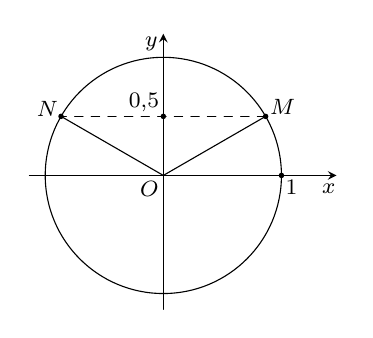
\begin{tikzpicture}[scale=1,>=stealth,font=\footnotesize,line join=round,line cap=round]
		\draw[->]  (-1.7,0)--(2.2,0) node[shift={(-120:.2)},scale=1]{$x$};
		\draw[->] (0,-1.7)--(0,1.8)  node[shift={(220:.2)},scale=1]{$y$};
		\path (0,0) coordinate  (O) node[shift={(-135:.25)},scale=1]{$O$};
		\draw (O) circle (1.5cm); 
		 \path
			(30:1.5) coordinate (M) 
			 (150:1.5) coordinate (N);
		 \draw[dashed](M)--(N);
		\draw  (M)--(O)--(N);
		\fill (M) node[shift={(30:.25)}]{$M$}circle (1pt); 
		\fill (N) node[shift={(150:.2)}]{$N$}circle (1pt); 
		\fill (0,0.75)  node[shift={(145:.3)}]{$0{,}5$}circle (1pt);
		 \fill (1.5,0) node[shift={(-50:.2)}]{$1$}circle (1pt);
	\end{tikzpicture}
		 }
	\loigiai{ 
		Ta thấy $2$ điểm $M$ và $N$ là các giao điểm của đường thẳng vuông góc với trục tung tại điểm $\dfrac{1}{2}$ với đường tròn lượng giác nên $M$ và $N$ là các điểm biểu diễn tập nghiệm của phương trình lượng giác cơ bản $\sin x=\dfrac{1}{2}\Leftrightarrow 2\sin  x=1$.
	} 
\end{ex}

% nguồn: Ok_Toan11_TracNghiem_Lan2
\begin{ex}%[1D1H5-3]%[ma:ea538e69]
	Chọn khẳng định \textbf{sai} trong các khẳng  định sau
	\choice 
		{$\cos x=1\Leftrightarrow x=k2\pi,  k\in\mathbb{Z}$}
		 {$\sin x=-1\Leftrightarrow x=-\dfrac{\pi}{2}+k2\pi, k\in\mathbb{Z}$}
		{\True  $\tan x=0\Leftrightarrow x=k2\pi, k\in\mathbb{Z}$}
		{$\cot x=0\Leftrightarrow  x=\dfrac{\pi}{2}+k\pi, k\in\mathbb{Z}$}
	 \loigiai{
		Ta có $\tan  x=0\Leftrightarrow x=k\pi, k\in\mathbb{Z}$.\\
		 Vậy khẳng định $\tan x=0\Leftrightarrow x=k2\pi, k\in\mathbb{Z}$ là sai.
	} 
\end{ex}

% nguồn: Ok_Toan11_TracNghiem_Lan2
\begin{ex}%[1D1H5-3]%[ma:07919ad3]
	Phương  trình $\cos x=-\dfrac{\sqrt{3}}{2}$ có tập nghiệm là
	\choice 
		 {$\left\{x= \pm \dfrac{\pi}{3}+k \pi \,\mid dle|\, k \in \mathbb{Z}\right\}$}
		{$\left\{x= \pm \dfrac{\pi}{6}+k \pi  \,\mid dle|\, k \in \mathbb{Z}\right\}$}
		{\True $\left\{x= \pm \dfrac{5 \pi}{6}+k 2 \pi \,\mid dle|\, k \in  \mathbb{Z}\right\}$}
		{$\left\{x= \pm \dfrac{\pi}{3}+k 2 \pi \,\mid  dle|\, k \in \mathbb{Z}\right\}$}
	\loigiai{ 
		 Ta có $\cos x=-\dfrac{\sqrt{3}}{2}
		 \Leftrightarrow \cos x=\cos \left(\dfrac{5 \pi}{6}\right)
		\Leftrightarrow x=  \pm \dfrac{5 \pi}{6}+k 2 \pi$, $k \in \mathbb{Z}$.
	} 
\end{ex}

% nguồn: Ok_Toan11_TracNghiem_Lan2
\begin{ex}%[1D1H5-3]%[ma:40115e5a]
	Giải phương  trình $\cot \left( 3x-1 \right)=-\sqrt{3}$.
	\choice 
		 {$x=\dfrac{1}{3}-\dfrac{\pi}{6}+k\pi $, $k\in\mathbb{Z}$}
		{$x=\dfrac{5\pi}{8}+\dfrac{k\pi}{3}$, $k\in\mathbb{Z}$} 
		 {$x=\dfrac{1}{3}+\dfrac{\pi}{18}+\dfrac{k\pi}{3}$, $k\in\mathbb{Z}$}
		{\True $x=\dfrac{1}{3}+\dfrac{5\pi}{18}+\dfrac{k\pi}{3}$, $k\in\mathbb{Z}$} 
	\loigiai{Ta có $\cot \left( 3x-1 \right)=-\sqrt{3}\Leftrightarrow 3x-1=\dfrac{5\pi}{6}+k\pi  \Leftrightarrow x=\dfrac{1}{3}+\dfrac{5\pi}{18}+\dfrac{k\pi}{3}$, $k\in\mathbb{Z}$.}
\end{ex}

% nguồn: Ok_Toan11_TracNghiem_Lan2
\begin{ex}%[1D1H5-3]%[ma:7edba3c0]
	Nghiệm của phương trình $\cot \left( x+2 \right)=1$  là
	\choice 
		{$x=2+\dfrac{\pi}{4}+k2\pi  $, $k\in \mathbb{Z}$}
		{\True  $x=-2+\dfrac{\pi}{4}+k\pi $, $k\in \mathbb{Z}$}
		{$x=-2-\dfrac{\pi}{4}+k\pi $, $k\in  \mathbb{Z}$}
		{$x=2+\dfrac{\pi}{4}+k\pi $, $k\in  \mathbb{Z}$}
	\loigiai{Ta có $\cot  \left( x+2 \right)=1\Leftrightarrow \cot \left( x+2 \right)=\cot \dfrac{\pi}{4}\Leftrightarrow x=-2+\dfrac{\pi}{4}+k\pi $ với $k\in \mathbb{Z}$.}
\end{ex}

% nguồn: Ok_Toan11_TracNghiem_Lan2
\begin{ex}%[1D1H5-3]%[ma:4db489e0]
	 Phương trình $\sin \left( x - \dfrac{\pi}{3} \right) = 1$ có nghiệm là
	 \choice
		{$x  = \dfrac{\pi}{3} + k2\pi$, $k \in \mathbb{Z}$}
		{$x = \dfrac{5\pi}{6} + k\pi$, $k \in  \mathbb{Z}$}
		 {\True $x = \dfrac{5\pi}{6} + k2\pi$, $k \in \mathbb{Z}$}
		{$x = \dfrac{\pi}{3} + 2\pi$, $k  \in \mathbb{Z}$}
	 \loigiai{
		Ta có 
		\begin{align*}
			\sin \left( x - \dfrac{\pi}{3} \right) = 1 \Leftrightarrow x - \dfrac{\pi}{3} = \dfrac{\pi}{2} + k2\pi \Leftrightarrow x = \dfrac{5\pi}{6} + k2\pi \, ,k  \in \mathbb{Z}.
		\end{align*}
		Vậy phương trình có nghiệm là  $x = \dfrac{5\pi}{6} + k2\pi$, $k \in \mathbb{Z}$.
	} 
\end{ex}

% nguồn: Ok_Toan11_TracNghiem_Lan2
\begin{ex}%[1D1H5-3]%[ma:1f996bf5]
	Số nghiệm của phương trình $2\sin x-\sqrt{3}=0$ trên đoạn $[0;2\pi]$  là
	 \choice
		{$3$} 
		 {$1$}
		{$4$} 
		 {\True $2$}
	\loigiai{ 
		Ta có 
		 \allowdisplaybreaks
		\begin{eqnarray*}
			 &&2\sin x-\sqrt{3}=0\\
			&\Leftrightarrow& \sin  x=\dfrac{\sqrt{3}}{2}\\
			&\Leftrightarrow& \sin x=\sin\left(\dfrac{\pi}{3}\right)\\ 
			&\Leftrightarrow& \hoac{ 
			&  x=\dfrac{\pi}{3}+k2\pi\\
			& x=\dfrac{2\pi}{3}+k2\pi 
			} (k\in\mathbb{Z}). 
		\end{eqnarray*}
		\begin{itemize}
			\item {\bfseries  Trường hợp 1:} $x=\dfrac{\pi}{3}+k2\pi$ $(k\in\mathbb{Z})$.\\
			$0\le x\le  2\pi$ $\Leftrightarrow$ $0\le\dfrac{\pi}{3}+k2\pi\le 2\pi$ $\Leftrightarrow$ $-\dfrac{\pi}{3}\le k2\pi\le\dfrac{5\pi}{3}$ $\Leftrightarrow$ $-\dfrac{1}{6}\le k\le\dfrac{5}{6}$. Suy ra $k=0$. Khi đó, $x=\dfrac{\pi}{3}$.
			\item {\bfseries Trường hợp  2:} $x=\dfrac{2\pi}{3}+k2\pi$ $(k\in\mathbb{Z})$.\\
			$0\le x\le 2\pi$  $\Leftrightarrow$ $0\le\dfrac{2\pi}{3}+k2\pi\le 2\pi$ $\Leftrightarrow$ $-\dfrac{2\pi}{3}\le k2\pi\le\dfrac{4\pi}{3}$ $\Leftrightarrow$ $-\dfrac{1}{3}\le k\le\dfrac{2}{3}$. Suy ra $k=0$. Khi đó, $x=\dfrac{2\pi}{3}$.
		\end{itemize}
		 Vậy phương trình đã cho có $2$ nghiệm thuộc đoạn $[0;2\pi]$.
	} 
\end{ex}

% nguồn: Ok_Toan11_TracNghiem_Lan2
\begin{ex}%[1D1H5-3]%[ma:eb6bde9a]
	Phương trình  $2\sin x-\sqrt{3}=0$ có tập nghiệm là
	\choice 
		{$\left\{\pm\dfrac{\pi}{6}+k2\pi ,k\in\mathbb{Z}\right\}$} 
		{$\left\{\pm\dfrac{\pi}{3}+k2\pi  ,k\in\mathbb{Z}\right\}$}
		 {$\left\{\dfrac{\pi}{6}+k2\pi;\dfrac{5\pi}{6}+k2\pi ,k\in\mathbb{Z}\right\}$}
		{\True  $\left\{\dfrac{\pi}{3}+k2\pi;\dfrac{2\pi}{3}+k2\pi ,k\in\mathbb{Z}\right\}$}
	\loigiai{ 
		Ta có $2\sin  x-\sqrt{3}=0\Leftrightarrow\sin x=\dfrac{\sqrt{3}}{2}\Leftrightarrow\hoac{&x=\dfrac{\pi}{3}+k2\pi\\&x=\dfrac{2\pi}{3}+k2\pi}\,(k\in\mathbb{Z})$.\\
		Vậy tập nghiệm  của phương trình là $S=\left\{\dfrac{\pi}{3}+k2\pi;\dfrac{2\pi}{3}+k2\pi ,k\in\mathbb{Z}\right\}$.
	 }
\end{ex}

% nguồn: Ok_Toan11_TracNghiem_Lan2
\begin{ex}%[1D1H5-3]%[ma:7deb4f75]
	Phương trình  $\cos 2 x+\cos x=0$ có bao nhiêu nghiệm thuộc khoảng $(-\pi; \pi)$?
	 \choice
		{\True $2$} 
		{$3$} 
		{$1$} 
		 {$4$}
	 \loigiai{
		Ta có $\cos 2 x+\cos x=0 \Leftrightarrow \cos 2 x=\cos (\pi+x) \Leftrightarrow\hoac{&x=\pi+k 2 \pi \\& x=-\dfrac{\pi}{3}+k \dfrac{2  \pi}{3}}$, $(k \in \mathbb{Z}).$\\
	Vì $-\pi<x<\pi  \Rightarrow\hoac{&x=-\dfrac{\pi}{3}\\& x=\dfrac{\pi}{3}.}$}
\end{ex}

% nguồn: Ok_TracNghiemLop11_Lan1
\begin{ex}%[1D1H5-3]%[ma:948958cc]
	Tổng $T$ các  nghiệm của phương trình $\sin x=\dfrac{1}{2}$ trên $(0;3\pi)$ bằng
	\choice 
		{$T=3\pi$} 
		{$T=\pi$} 
		 {$T=5\pi$}
		{\True $T=6\pi$} 
	\loigiai{ 
		Ta có $\sin x=\dfrac{1}{2}=\sin \dfrac{\pi}{6}\Leftrightarrow \hoac{&x=\dfrac{\pi}{6}+k2\pi\\&x=\dfrac{5\pi}{6}+k2\pi}$.\\ 
		Do $x\in (0;3\pi)$ nên các nghiệm của phương trình là $x=\dfrac{\pi}{6}$,  $x=\dfrac{13\pi}{6}$, $x=\dfrac{5\pi}{6}$, $x=\dfrac{17\pi}{6}$. Suy ra tổng các nghiệm là $T=6\pi$.
	 }
\end{ex}

% nguồn: Ok_TracNghiemLop11_Lan1
\begin{ex}%[1D1H5-3]%[ma:ffa3687f]
	Tìm tất cả các giá trị thực của  tham số $m$để phương trình $\sin x=m$ có nghiệm thực.
	\choice 
		 {$m\ge 0$}
		 {\True $-1\le m\le 1$}
		{$-1<m<1$} 
		 {$m>0$}
	\loigiai{ 
		Do $-1\le \sin x\le 1,\text{ }\forall x\in \mathbb{R}$ nên phương trình $\sin x=m$ có nghiệm khi và chỉ khi $-1\le  m\le 1$.
	} 
\end{ex}

% nguồn: Ok_TracNghiemLop11_Lan1
\begin{ex}%[1D1H5-3]%[ma:3e293feb]
	Số nghiệm của phương trình $\tan x=3$ trong khoảng  $\left(-\dfrac{\pi}{2};\dfrac{7 \pi}{3}\right)$ là
	\choice 
		{$1$} 
		{\True  $2$}
		{$3$} 
		{$4$} 
	\loigiai{ 
		\textbf{Cách 1:} Giải  bằng máy tính cầm tay\\
		Ta  có
		\allowdisplaybreaks 
		\begin{eqnarray*}
			\tan  x=3\Leftrightarrow x\approx 1{,}249+k\pi \quad (k\in\mathbb{Z}).
		\end{eqnarray*}
		Cho $-\dfrac{\pi}{2}<1{,}249+k\pi<\dfrac{7\pi}{3}\Rightarrow -0{,}89<k<  1{,}94$.\\
		Vì $k\in\mathbb{Z}$ nên $k\in \{0;1\}$. Có $2$ giá trị $k$, tương ứng với  $2$ nghiệm $x$ nằm trong khoảng đã cho.\\
		\textbf{Cách 2:} Dựa vào đồ  thị\\
		Ta có  đồ thị hàm số $y=\tan x$ trong khoảng $\left(-\dfrac{\pi}{2};\dfrac{7\pi}{3}\right)$ như sau:
		\begin{center}
			\begin{tikzpicture}[font=\footnotesize,line join=round,line cap=round,>=stealth,scale=.7]
					\def\xmin{-.8*pi} 
					\def\xmax{3*pi} 
					 \def\ymin{-5}
					\draw[->] (\xmin,0)--(0,0) node[above left]{$O$}--(\xmax,0)  node[above]{$x$};
					\draw[->] (0,\ymin)--(0,-\ymin) node[left]{$y$}; 
				\foreach \batdau/\ketthuc in { 
					 {-pi/2+.2}/{pi/2-.2},{.5*pi+.2}/{1.5*pi-.2},{1.5*pi+.2}/{7*pi/3}
					 }{
					\draw[domain=\batdau:\ketthuc,samples=100,smooth] plot (\x,{tan (\x r)}); 
				} 
				\draw  (\xmin,3)--(\xmax,3) node[above]{$y=3$};
				 \foreach \x in {-.5,.5,1.5}{
					\draw[dashed] (\x*pi,\ymin)--++(0,-2*\ymin); 
				 }
				\draw[dashed]  (7*pi/3,0) node[below]{$\tfrac{7\pi}{3}$}--++(0,{sqrt (3)})--++({-7*pi/3},0) node[left]{$\sqrt{3}$};
				\foreach  \co/\no in {
					(-.5*pi,0)/-\tfrac{\pi}{2},(.5*pi,0)/\tfrac{\pi}{2},(1.5*pi,0)/\tfrac{3\pi}{2} 
					}{ 
					\draw[fill] \co node[below  left]{$\no$} circle (1pt);
				 }
				 \draw[fill]
					 (7*pi/3,{sqrt (3)}) circle (1pt)
					(0,0) circle (1pt); 
			\end{tikzpicture}
		\end{center}
		Từ đó suy ra phương trình $\tan x=3$ có $2$ nghiệm trong khoảng  $\left(-\dfrac{\pi}{2};\dfrac{\pi}{3}\right)$.
	 }
\end{ex}

% nguồn: Ok_TracNghiemLop11_Lan1
\begin{ex}%[1D1H5-3]%[ma:1f6e01f2]
	Tất cả nghiệm của  phương trình $2\cos x+1=0$ là
	\choice 
		{$x=\pm\dfrac{2\pi}{3}+k\pi$, $k  \in \mathbb{Z}$}
		{$x=\pm\dfrac{\pi}{3}+k\pi$,  $k \in \mathbb{Z}$}
		 {$x=\pm\dfrac{\pi}{3}+k2\pi$, $k \in \mathbb{Z}$}
		 {\True $x=\pm\dfrac{2\pi}{3}+k2\pi$, $k \in \mathbb{Z}$}
	 \loigiai{
		Ta  có $2\cos x+1=0$ $\Leftrightarrow\cos x=-\dfrac{1}{2}\Leftrightarrow\cos x=\cos\dfrac{2\pi}{3} \Leftrightarrow x=\pm\dfrac{2\pi}{3}+k2\pi$, $k \in \mathbb{Z}$.
	} 
\end{ex}

% nguồn: Ok_TracNghiemLop11_Lan1
\begin{ex}%[1D1H5-3]%[ma:39711849]
	Nghiệm của phương trình $\cos x=-\dfrac{1}{2}$  là
	\choice 
		 {\True $x=\pm \dfrac{2\pi }{3}+k2\pi $}
		 {$x=\pm \dfrac{\pi }{6}+k\pi $}
		{$x=\pm \dfrac{\pi }{3}+k2\pi  $}
		{$x=\pm \dfrac{\pi  }{6}+k2\pi $}
	 \loigiai{
		Ta có  $\cos x=-\dfrac{1}{2}\Leftrightarrow \cos x=\cos \left( -\dfrac{2\pi }{3}\right) \Leftrightarrow x=\pm \dfrac{2\pi }{3}+k2\pi.$\\
		Vậy  phương trình có các nghiệm là $x=\pm \dfrac{2\pi }{3}+k2\pi \left( k\in \mathbb{Z} \right)$.
	} 
\end{ex}

% nguồn: Ok_TracNghiemLop11_Lan1
\begin{ex}%[1D1H5-3]%[ma:3a47c8ff]
	Tìm nghiệm của phương trình $\tan  (2x)=1$.
	\choice 
		{$x=\dfrac{\pi}{4}+k\pi,k\in \mathbb{Z}$} 
		{$x=\dfrac{\pi}{8}+k\pi,k\in  \mathbb{Z}$}
		{\True  $x=\dfrac{\pi}{8}+k\dfrac{\pi}{2}$, $k\in \mathbb{Z}$}
		{$x=\dfrac{\pi}{4}+k\dfrac{\pi}{2}$, $k\in \mathbb{Z}$} 
	 \loigiai{
		$\tan (2x)=1\Leftrightarrow 2x=\dfrac{\pi}{4}+k\pi \Leftrightarrow x=\dfrac{\pi}{8}+k\dfrac{\pi}{2}$,  $k\in \mathbb{Z}$.
	} 
\end{ex}

% nguồn: Ok_TracNghiemLop11_Lan1
\begin{ex}%[1D1H5-3]%[ma:e29e4e3c]
	Phương trình $\cos x=-\dfrac{\sqrt{3}}{2}$ có tập  nghiệm là
	 \choice
		{$\left\{ x=\pm \dfrac{\pi  }{6}+k\pi; k\in \mathbb{Z} \right\}$}
		{\True $\left\{ x=\pm \dfrac{5\pi }{6}+k2\pi; k\in \mathbb{Z} \right\}$} 
		{$\left\{ x=\pm \dfrac{\pi }{3}+k\pi;  k\in \mathbb{Z} \right\}$}
		{$\left\{ x=\pm \dfrac{\pi }{3}+k2\pi; k\in \mathbb{Z} \right\}$} 
	 \loigiai{
		Ta có $\cos x=-\dfrac{\sqrt{3}}{2}$$\Leftrightarrow \cos x=\cos \dfrac{5\pi }{6}$$\Leftrightarrow x=\pm \dfrac{5\pi  }{6}+k2\pi ,k\in \mathbb{Z}$.
	 }
\end{ex}

% nguồn: Ok_TracNghiemLop11_Lan1
\begin{ex}%[1D1H5-3]%[ma:f56d73c5]
	Tập  nghiệm của phương trình $\tan x+1=0$ là
	\choice 
		{$S=\left\{ -\dfrac{\pi }{4}+k2\pi ,k\in \mathbb{Z} \right\}$} 
		{$S=\left\{ \dfrac{\pi  }{4}+k\pi ,k\in \mathbb{Z} \right\}$}
		{\True $S=\left\{ -\dfrac{\pi }{4}+k\pi ,k\in \mathbb{Z} \right\}$} 
		{$S=\left\{ \dfrac{\pi }{4}+k2\pi ,k\in \mathbb{Z}  \right\}$}
	\loigiai{ 
		Ta có $\tan x+1=0$$\Leftrightarrow \tan x=-1$ $\Leftrightarrow x=-\dfrac{\pi }{4}+k\pi ,k\in  \mathbb{Z}$.
	} 
\end{ex}

% nguồn: Ok_TracNghiemLop11_Lan1
\begin{ex}%[1D1H5-3]%[ma:37ab5cb8]
	Tìm tập nghiệm  $S$ của phương trình $\cos 2x=-\dfrac{\sqrt{2}}{2}$.
	\choice 
		{$S=\left\{ -\dfrac{3\pi }{8}+k2\pi;\dfrac{3\pi }{8}+k2\pi ,k\in  \mathbb{Z} \right\}$}
		{\True $S=\left\{ -\dfrac{3\pi  }{8}+k\pi;\dfrac{3\pi }{8}+k\pi ,k\in \mathbb{Z} \right\}$}
		{$S=\left\{ \dfrac{3\pi  }{8}+k\pi;\dfrac{\pi }{8}+k\pi ,k\in \mathbb{Z} \right\}$}
		{$S=\left\{ \dfrac{3\pi }{8}+k2\pi;\dfrac{\pi }{8}+k2\pi ,k\in \mathbb{Z}  \right\}$}
	 \loigiai{
		Ta có $\cos 2x=-\dfrac{\sqrt{2}}{2}\Leftrightarrow \left[\begin{aligned}
		&  2x=\dfrac{3\pi }{4}+k2\pi \\
		& 2x=-\dfrac{3\pi }{4}+k2\pi  \\
	\end{aligned} \right.\Leftrightarrow \left[\begin{aligned}
	 & x=\dfrac{3\pi }{8}+k\pi \\
	 & x=-\dfrac{3\pi }{8}+k\pi \\
	\end{aligned} \right.\left( k\in \mathbb{Z} \right).$\\
	Vậy tập  nghiệm của phương trình trên là $S=\left\{ -\dfrac{3\pi }{8}+k\pi;\dfrac{3\pi }{8}+k\pi ,k\in \mathbb{Z} \right\}.$
 }
\end{ex}

% nguồn: Ok_TracNghiemLop11_Lan1
\begin{ex}%[1D1H5-3]%[ma:40cd489d]
	Tập nghiệm của phương  trình $3\cos\left( 3x-\dfrac{\pi }{3} \right)=0$ là
	 \choice
		{$\left\{ \dfrac{\pi }{2}+k\pi ,k\in \mathbb{Z}  \right\}$}
		 {\True $\left\{ \dfrac{5\pi }{18}+\dfrac{k\pi }{3},k\in \mathbb{Z} \right\}$}
		 {$\left\{ \dfrac{5\pi }{6}+k2\pi ,k\in \mathbb{Z} \right\}$}
		 {$\left\{ \dfrac{5\pi }{18}+\dfrac{k2\pi }{3},k\in \mathbb{Z} \right\}$}
	\loigiai{ 
		Ta có $3\cos\left(  3x-\dfrac{\pi }{3} \right)=0\Leftrightarrow \cos\left( 3x-\dfrac{\pi }{3} \right)=0\Leftrightarrow 3x-\dfrac{\pi }{3}=\dfrac{\pi }{2}+k\pi \Leftrightarrow x=\dfrac{5\pi }{18}+\dfrac{k\pi }{3}$.
	} 
\end{ex}

% nguồn: Ok_TracNghiemLop11_Lan1
\begin{ex}%[1D1H5-3]%[ma:0a3fc748]
	Phương trình $\cot \left( x+45^\circ \right)=\dfrac{\sqrt{3}}{3}$ có nghiệm là (với $k\in \mathbb{Z}$) 
	 \choice
		{\True $15^\circ  +k180{}^\circ $}
		{$30^\circ +k180{}^\circ $} 
		{$45^\circ +k180^\circ $} 
		{$60^\circ +k180^\circ $} 
	 \loigiai{
		Phương trình $\cot \left( x+45^\circ \right)=\dfrac{\sqrt{3}}{3}$ $\Leftrightarrow \cot \left( x+45^\circ \right)=\cot 60{}^\circ  $ $\Leftrightarrow x+45{}^\circ =60^\circ +k180^\circ $
		$\Leftrightarrow x=15{}^\circ +k180^\circ $ (  với $k\in \mathbb{Z}$).
	} 
\end{ex}

% nguồn: Ok_TracNghiemLop11_Lan1
\begin{ex}%[1D1H5-3]%[ma:8e373f96]
	Nghiệm của phương trình $\sqrt{3}+3\tan  x=0$ là
	 \choice
		{$x=\dfrac{\pi }{3}+k\pi  $}
		{$x=\dfrac{\pi }{2}+k2\pi  $}
		{\True $x=-\dfrac{\pi }{6}+k\pi $} 
		 {$x=\dfrac{\pi }{2}+k\pi $}
	\loigiai{ 
		Ta có $\sqrt{3}+3\tan x=0\Leftrightarrow \tan x=-\dfrac{\sqrt{3}}{3}\Leftrightarrow x=-\dfrac{\pi }{6}+k\pi \left( k\in \mathbb{Z}  \right)$.
	 }
\end{ex}

% nguồn: Ok_TracNghiemLop11_Lan1
\begin{ex}%[1D1H5-3]%[ma:ccd58263]
	Với $x\in[-\pi;\pi]$, phương trình $\cos x=\dfrac{\sqrt{3}}{2}$  có bao nhiêu nghiệm?
	\choice 
		 {$1$}
		{\True  $2$}
		 {$3$}
		 {$4$}
	 \loigiai{
		 Ta có $\cos x=\dfrac{\sqrt{3}}{2} \Leftrightarrow \cos x=\cos\dfrac{\pi}{6} \Leftrightarrow \hoac{&x=\dfrac{\pi}{6}+k2\pi\\&x=-\dfrac{\pi}{6}+k2\pi} ,(k\in\mathbb{Z})$. \\
	Vì $x\in[-\pi;\pi]$  nên phương trình đã cho chỉ có $2$ nghiệm là $x=-\dfrac{\pi}{6};x=\dfrac{\pi}{6}$}.
\end{ex}

% nguồn: Ok_TracNghiemLop11_Lan1
\begin{ex}%[1D1H5-3]%[ma:2c96170e]
	Tất cả các nghiệm của  phương trình $\sin 2x=\dfrac{\sqrt{2}}{2}$ là
	 \choice
		{$\hoac{&x=\dfrac{\pi}{4}+k2\pi\\&x=\dfrac{3\pi}{4}+k2\pi} \left(k\in \mathbb{Z}\right)$} 
		{$\hoac{&x=\dfrac{\pi}{4}+k\pi\\&x=\dfrac{3\pi}{4}+k\pi}  \left(k\in \mathbb{Z}\right)$}
		{\True $\hoac{&x=\dfrac{\pi}{8}+k\pi\\&x=\dfrac{3\pi}{8}+k\pi} \left(k\in  \mathbb{Z}\right)$}
		{$\hoac{&x=\dfrac{\pi}{8}+k2\pi\\&x=\dfrac{3\pi}{8}+k2\pi} \left(k\in  \mathbb{Z}\right)$}
	 \loigiai{
		Ta  có
		 \allowdisplaybreaks
		\begin{eqnarray*}
			 &&\sin 2x=\dfrac{\sqrt{2}}{2}\\
			 &\Leftrightarrow&\sin 2x=\sin\dfrac{\pi}{4}\\
			&\Leftrightarrow&\hoac{&2x=\dfrac{\pi}{4}+k2\pi\\&2x=\pi-\dfrac{\pi}{4}+k2\pi}\\ 
			 &\Leftrightarrow&\hoac{&x=\dfrac{\pi}{8}+k\pi\\&x=\dfrac{3\pi}{8}+k\pi} \left(k\in \mathbb{Z}\right).
		\end{eqnarray*}
	} 
\end{ex}

% nguồn: Ok_TracNghiemLop11_Lan1
\begin{ex}%[1D1H5-3]%[ma:d96fbb40]
	 Nghiệm của phương trình $\sin 2x=1$ là
	 \choice
		{\True $x=\dfrac{\pi }{4}+k\pi  $}
		{$x=\dfrac{\pi  }{4}+k2\pi $}
		{$x=\dfrac{k\pi }{2}$} 
		{$x=\dfrac{\pi }{2}+k2\pi $} 
	 \loigiai{
		Ta có $\sin 2x=1$$\Leftrightarrow 2x=\dfrac{\pi }{2}+k2\pi  $$\Leftrightarrow x=\dfrac{\pi }{4}+k\pi $.
	 }
\end{ex}

% nguồn: Ok_TracNghiemLop11_Lan1
\begin{ex}%[1D1H5-3]%[ma:ab3b951a]
	Phương  trình $\cos x=\cos\dfrac{\pi}{3}$ có tất cả các nghiệm là
	\choice 
		{$x=\dfrac{2\pi}{3}+k2\pi  $, $\left(k\in\mathbb{Z}\right)$}
		{$x=\pm\dfrac{\pi}{3}+k\pi $,  $\left(k\in\mathbb{Z}\right)$}
		{\True $x=\pm\dfrac{\pi}{3}+k2\pi$,  $\left(k\in\mathbb{Z}\right)$}
		{$x=\dfrac{\pi}{3}+k2\pi $,  $\left(k\in\mathbb{Z}\right)$}
	 \loigiai{
	Áp dụng  công thức nghiệm, phương trình $\cos x=\cos\dfrac{\pi}{3}$ có tất cả các nghiệm là $$x=\pm\dfrac{\pi}{3}+k2\pi,\ \left(k\in\mathbb{Z}\right).$$}
\end{ex}

% nguồn: Ok_TracNghiemLop11_Lan1
\begin{ex}%[1D1H5-3]%[ma:363915bd]
	Nghiệm của phương  trình $\cos x=- \dfrac{1}{2}$ là
	 \choice
		{\True $x=\pm  \dfrac{2\pi }{3}+k2\pi $}
		 {$x=\pm \dfrac{\pi }{6}+k\pi $}
		{$x=\pm \dfrac{\pi }{3}+k2\pi $} 
		{$x=\pm \dfrac{\pi }{6}+k2\pi  $}
	 \loigiai{
		Ta có  $\cos x=- \dfrac{1}{2}\Leftrightarrow \cos x=\cos \dfrac{2\pi }{3}\Leftrightarrow x=\pm \dfrac{2\pi }{3}+k2\pi ,k\in \mathbb{Z}$.
	 }
\end{ex}

% nguồn: Ok_TracNghiemLop11_Lan1
\begin{ex}%[1D1H5-3]%[ma:241dea3b]
	Nghiệm của phương trình $\cos x=\dfrac{1}{2}$  là
	\choice 
		{\True $\left[\begin{aligned}
		 & x=\dfrac{\pi }{6}+k2\pi \\
		& x=-\dfrac{\pi }{6}+k2\pi . \\ 
\end{aligned} \right.,k\in \mathbb{Z}$}
{$\left[\begin{aligned}
 & x=\dfrac{\pi }{6}+k2\pi \\
 & x=\dfrac{5\pi }{6}+k2\pi \\
\end{aligned} \right.,k\in \mathbb{Z}$}
{$\left[\begin{aligned}
&  x=\dfrac{\pi }{3}+k2\pi \\
&  x=\dfrac{2\pi }{3}+k2\pi \\
\end{aligned} \right.,k\in \mathbb{Z}$}
{$\left[\begin{aligned}
& x=\dfrac{\pi }{3}+k2\pi  \\
& x=-\dfrac{\pi }{3}+k2\pi \\ 
\end{aligned} \right.,k\in \mathbb{Z}$}
\loigiai{ 
	Ta có $\cos x=\dfrac{1}{2}\Leftrightarrow \cos x=\cos \dfrac{\pi }{6}\Leftrightarrow \left[\begin{aligned}
	& x=\dfrac{\pi }{6}+k2\pi \\ 
	& x=-\dfrac{\pi  }{6}+k2\pi \\
	\end{aligned} \right.,k\in \mathbb{Z}$.
} 
\end{ex}

% nguồn: Ok_TracNghiemLop11_Lan1
\begin{ex}%[1D1H5-3]%[ma:1ea40165]
	Nghiệm  của phương trình $\sqrt{3}\cot x-3=0$ là
	\choice 
		{$x=\dfrac{\pi  }{3}+k2\pi \left( k\in \mathbb{Z} \right)$}
		{$x=\dfrac{\pi }{3}+k\pi \left( k\in \mathbb{Z}  \right)$}
		{\True $x=\dfrac{\pi }{6}+k\pi  \left( k\in \mathbb{Z} \right)$}
		{$x=\dfrac{\pi }{6}+k2\pi \left( k\in \mathbb{Z} \right)$} 
	\loigiai{ 
		Ta có $\sqrt{3}\cot x-3=0\Leftrightarrow \cot x=\sqrt{3}\Leftrightarrow x=\dfrac{\pi }{6}+k\pi \left( k\in  \mathbb{Z} \right)$.
	} 
\end{ex}

% nguồn: Ok_TracNghiemLop11_Lan1
\begin{ex}%[1D1H5-3]%[ma:10784e7c]
	Biểu diễn  họ nghiệm của phương trình $\sin2x=1$ trên đường tròn đơn vị ta được bao nhiêu điểm?
	 \choice
		 {$1$}
		 {$8$}
		 {$4$}
		{\True  $2$}
	 \loigiai{
		 Ta có $\sin2x=1\Leftrightarrow 2x=\dfrac{\pi}{2}+2k\pi\Leftrightarrow x=\dfrac{\pi}{4}+k\pi,\,k\in \mathbb{Z}$.\\
		Vậy có $2$ điểm trên đường tròn đơn vị. 
	} 
\end{ex}

% nguồn: Ok_TracNghiemLop11_Lan1
\begin{ex}%[1D1H5-3]%[ma:6d248636]
	Nghiệm của phương trình $2\cos x-1=0$  là
	\choice 
		{$x=\pm \dfrac{2\pi}{3}+k2\pi,k\in  \mathbb{Z}$}
		{$x=\pm  \dfrac{\pi}{6}+k\pi,k\in \mathbb{Z}$}
		 {\True $x=\pm \dfrac{\pi}{3}+k2\pi,k\in \mathbb{Z}$}
		{$x=\pm \dfrac{\pi}{6}+k2\pi,k\in  \mathbb{Z}$}
	\loigiai{ 
		Ta  có $2\cos x-1=0\Leftrightarrow \cos x=\dfrac{1}{2}\Leftrightarrow \cos x=\cos \dfrac{\pi}{3}\Leftrightarrow x=\pm \dfrac{\pi}{3}+k2\pi,k\in \mathbb{Z}$.
	 }
\end{ex}

% nguồn: Ok_TracNghiemLop11_Lan1
\begin{ex}%[1D1H5-3]%[ma:ad95a30e]
	Nghiệm của phương trình $\cos \left( x+\dfrac{\pi }{6} \right)=-\dfrac{1}{2}$  là
	\choice 
		{$\left[\begin{aligned}
		&  x=\dfrac{\pi }{2}+k2\pi \\
		& x=\dfrac{\pi }{3}+k2\pi \\ 
\end{aligned} \right.\left( k\in \mathbb{Z} \right)$}
{\True $\left[\begin{aligned}
& x=\dfrac{\pi  }{2}+k2\pi \\
& x=-\dfrac{5\pi }{6}+k2\pi \\ 
\end{aligned} \right.\left( k\in \mathbb{Z} \right)$}
{$\left[\begin{aligned}
& x=\dfrac{\pi }{2}+k2\pi  \\
 & x=\dfrac{\pi }{6}+k2\pi \\
\end{aligned} \right.\left( k\in \mathbb{Z} \right)$}
{$\left[\begin{aligned}
& x=\dfrac{\pi }{6}+k2\pi  \\
&  x=-\dfrac{5\pi }{6}+k2\pi \\
\end{aligned} \right.\left( k\in \mathbb{Z} \right)$}
\loigiai{ 
	Ta có $\cos \left( x+\dfrac{\pi }{6} \right)=-\dfrac{1}{2}\Leftrightarrow \left[\begin{aligned}
	& x+\dfrac{\pi }{6}=\dfrac{2\pi }{3}+k2\pi \\ 
	&  x+\dfrac{\pi }{6}=-\dfrac{2\pi }{3}+k2\pi \\
	\end{aligned} \right.\Leftrightarrow \left[\begin{aligned}
	&  x=\dfrac{\pi }{2}+k2\pi \\
	&  x=-\dfrac{5\pi }{6}+k2\pi \\
	\end{aligned} \right.\left( k\in \mathbb{Z} \right)$.
 }
\end{ex}

% nguồn: Ok_TracNghiemLop11_Lan1
\begin{ex}%[1D1H5-3]%[ma:87ac70e0]
	Giải phương  trình $\sin x=\dfrac{\sqrt{3}}{2}$.
	 \choice
		{$x= \pm \dfrac{\pi}{3}+k 2  \pi$, $k\in\mathbb{Z}$}
		{$x=\dfrac{\pi}{3}+k \pi$,  $k\in\mathbb{Z}$}
		{$\hoac{&x=\dfrac{\pi}{6}+k  \pi \\ &x=\dfrac{5 \pi}{6}+k \pi}$, $k\in\mathbb{Z}$}
		{\True $\hoac{&x=\dfrac{\pi}{3}+k 2 \pi \\ &x=\dfrac{2  \pi}{3}+k 2 \pi}$, $k\in\mathbb{Z}$}
	\loigiai{ 
	Ta có $\sin x  =\dfrac{\sqrt{3}}{2}
	\Leftrightarrow \sin x = \sin \dfrac{\pi}{3} 
	\Leftrightarrow  \hoac{&x=\dfrac{\pi}{3}+k2\pi\\&x=\dfrac{2\pi}{3}+k2\pi}$, $k\in\mathbb{Z}$.
	} 
\end{ex}

% nguồn: Ok_TracNghiemLop11_Lan1
\begin{ex}%[1D1H5-3]%[ma:2c899cba]
	Tập nghiệm  $S$ của phương trình $\cos 2x=0$ là
	\choice 
		{\True $S=\left\{\dfrac{\pi }{4}+k\dfrac{\pi  }{2}\big|k\in \mathbb{Z}\right\}$}
		{$S=\left\{\dfrac{\pi  }{4}+k\pi \big|k\in \mathbb{Z}\right\}$}
		{$S=\left\{\dfrac{\pi }{2}+k\pi  \big|k\in \mathbb{Z}\right\}$}
		 {$S=\left\{\dfrac{\pi }{4}+k2\pi \big|k\in \mathbb{Z}\right\}$}
	 \loigiai{
		Ta có $\cos 2x=0\Leftrightarrow  2x=\dfrac{\pi }{2}+k\pi \Leftrightarrow x=\dfrac{\pi }{4}+k\dfrac{\pi }{2},k\in \mathbb{Z}$.\\
	Vậy phương trình có tập nghiệm $S=\left\{\dfrac{\pi }{4}+k\dfrac{\pi }{2}\big|k\in \mathbb{Z}\right\}$.} 
\end{ex}

% nguồn: Ok_TracNghiemLop11_Lan1
\begin{ex}%[1D1H5-3]%[ma:279cb703]
	Tập nghiệm của phương trình  $\cot 2x=0$ là
	\choice 
		{$\left\{ \dfrac{\pi }{4}+k2\pi  |k\in \mathbb{Z} \right\}$}
		{$\left\{ \dfrac{\pi }{4}+k\pi |k\in \mathbb{Z} \right\}$} 
		{\True $\left\{  \dfrac{\pi }{4}+k\dfrac{\pi }{2}|k\in \mathbb{Z} \right\}$}
		{$\left\{ \dfrac{\pi }{4}+k4\pi |k\in \mathbb{Z}  \right\}$}
	 \loigiai{
		Ta  có $\cot 2x=0\Leftrightarrow 2x=\dfrac{\pi }{2}+k\pi \Leftrightarrow x=\dfrac{\pi }{4}+k\dfrac{\pi }{2}(k\in \mathbb{Z}).$
	} 
\end{ex}

% nguồn: Ok_TracNghiemLop11_Lan1
\begin{ex}%[1D1H5-3]%[ma:886ff8bc]
	Phương trình $2\cot x-\sqrt{3}=0$ có nghiệm là 
	\choice 
		{\True  $x=\text{arccot}\dfrac{\sqrt{3}}{2}+k\pi \left( k\in \mathbb{Z} \right)$}
		{$x=\dfrac{\pi  }{6}+k\pi \left( k\in \mathbb{Z} \right)$}
		{$\left[\begin{aligned}
		& x=\dfrac{\pi  }{6}+k2\pi \\
		 & x=-\dfrac{\pi }{6}+k2\pi \\
\end{aligned} \right.\left( k\in \mathbb{Z} \right)$}
{$x=\dfrac{\pi }{3}+k2\pi \left(  k\in \mathbb{Z} \right)$}
 \loigiai{
	Ta có $2\cot x-\sqrt{3}=0\Leftrightarrow \cot x=\dfrac{\sqrt{3}}{2}\Leftrightarrow x=\text{arccot}\dfrac{\sqrt{3}}{2}+k\pi \left( k\in  \mathbb{Z} \right)$.
} 
\end{ex}

% nguồn: Ok_TracNghiemLop11_Lan1
\begin{ex}%[1D1H5-3]%[ma:05272d4f]
	Tập nghiệm của phương trình  $2\cos x+\sqrt{3}=0$ là
	\choice 
		 {\True $\left\{ \pm \dfrac{5\pi }{6}+k2\pi |k\in \mathbb{Z} \right\}$}
		{$\left\{ \pm \dfrac{\pi }{6}+k2\pi |k\in \mathbb{Z}  \right\}$}
		{$\left\{ \pm \dfrac{\pi }{6}+k\pi |k\in \mathbb{Z} \right\}$} 
		{$\left\{ \pm  \dfrac{5\pi }{6}+k\pi |k\in \mathbb{Z} \right\}$}
	\loigiai{ 
		Ta có $2\cos x+\sqrt{3}=0\Leftrightarrow \cos x=-\dfrac{\sqrt{3}}{2}\Leftrightarrow x=\pm \dfrac{5\pi }{6}+k2\pi ,k\in  \mathbb{Z}$.
	} 
\end{ex}

% nguồn: Ok_TracNghiemLop11_Lan1
\begin{ex}%[1D1H5-3]%[ma:54f429c0]
	Nghiệm của phương trình  $\tan 2x+\sqrt{3}=0$ là
	 \choice
		{$x=\dfrac{\pi }{6}+k\pi  ,k\in \mathbb{Z}$}
		 {$x=-\dfrac{\pi }{6}+k\pi ,k\in \mathbb{Z}$}
		{$x=\dfrac{\pi }{6}+\dfrac{k\pi }{2},k\in  \mathbb{Z}$}
		{\True $x=-\dfrac{\pi }{6}+\dfrac{k\pi  }{2},k\in \mathbb{Z}$}
	 \loigiai{
		Ta có $\tan 2x+\sqrt{3}=0\Leftrightarrow \tan 2x=-\sqrt{3}\Leftrightarrow 2x=-\dfrac{\pi }{3}+k\pi $ $\Leftrightarrow x=-\dfrac{\pi }{6}+\dfrac{k\pi }{2},k\in \mathbb{Z}$. 
	 }
\end{ex}

% nguồn: Ok_TracNghiemLop11_Lan1
\begin{ex}%[1D1H5-3]%[ma:3ada8f45]
	Số  nghiệm của phương trình $\cos x=\dfrac{1}{2}$ thuộc đoạn $\left[-2\pi;2\pi\right]$ là
	\choice 
		{\True  $4$}
		{$2$} 
		{$3$} 
		 {$1$}
	\loigiai{Ta có$$\cos x=\dfrac{1}{2}\Leftrightarrow x=\pm \dfrac{\pi}{3}+k2\pi, k  \in \mathbb{Z}.$$
	Suy ra phương trình có $4$ nghiệm $\pm \dfrac{\pi}{3}; 2\pi  \pm \dfrac{\pi}{3}$ thuộc đoạn $\left[-2\pi;2\pi\right]$. }
\end{ex}

% nguồn: Ok_TracNghiemLop11_Lan1
\begin{ex}%[1D1H5-3]%[ma:edb21857]
	Phương trình $\cos x-m=0$ vô nghiệm khi giá  trị tham số $m$thỏa mãn.
	\choice 
		{\True $\left[\begin{aligned}
		&  m<-1 \\
		 & m>1 \\
\end{aligned} \right.$}
{$-1\le m\le 1$} 
{$m>1$} 
{$m<-1$} 
 \loigiai{
	Ta có $\cos  x-m=0\Leftrightarrow \cos x=m$.
	Phương trình vô nghiệm khi và chỉ khi $m\notin \left[-1;1 \right]$$\Leftrightarrow \left[\begin{aligned}
	&  m<-1 \\
	 & m>1.\\
	\end{aligned} \right.$
} 
\end{ex}

% nguồn: Ok_TracNghiemLop11_Lan1
\begin{ex}%[1D1H5-3]%[ma:009fa65e]
	 Phương trình nào sau đây có nghiệm?
	 \choice
		{$\cos  x=-\dfrac{3}{2}$}
		{$\sin x=\sqrt{2}$} 
		{\True $\tan x=3$} 
		{${\cos  }^{2}x-3=0$}
	\loigiai{ 
		Vì phương trình $\tan x=a$ luôn có nghiệm. 
	 }
\end{ex}

% nguồn: Ok_TracNghiemLop11_Lan1
\begin{ex}%[1D1H5-3]%[ma:9e052fc5]
	Số nghiệm của phương  trình $\cos \left(x+\dfrac{\pi}{3} \right)+1=0$ trên $\left[-\pi;2\pi \right)$ là
	\choice{$2$} 
		{$3$} 
		{$0$} 
		 {\True $1$}
	 \loigiai{
		Ta có 
		\allowdisplaybreaks 
		\begin{eqnarray*}
			&&\cos \left(x+\dfrac{\pi}{3}  \right)+1=0\\
			&\Leftrightarrow& \cos \left(x+\dfrac{\pi}{3} \right)=-1\\ 
			&\Leftrightarrow& x=\dfrac{2\pi}{3}+k2\pi,  k\in \mathbb{Z}.
		\end{eqnarray*}
		 Xét $x=\dfrac{2\pi}{3}+k2\pi$.\\
		Khi  đó
		 $$
		 -\pi \le x < 2\pi\Leftrightarrow-\pi \le \dfrac{2\pi}{3}+k2\pi < 2\pi
		\Leftrightarrow-\dfrac{5}{6} \le  k < \dfrac{2}{3}.
		 $$
		Vì $k\in \mathbb{Z}\Rightarrow  k=0$ nên $x=\dfrac{2\pi}{3}$.\\
	Vậy phương trình có $1$ nghiệm  trên $\left[-\pi;2\pi \right)$.}
\end{ex}

% nguồn: Ok_TracNghiemLop11_Lan1
\begin{ex}%[1D1H5-3]%[ma:dae392b2]
	 Giải phương trình $\sqrt{\text{3}}\tan 2x-3=0$.
	 \choice
		{$x=\dfrac{\pi }{3}+k\dfrac{\pi  }{2}\left( k\in \mathbb{Z} \right)$}
		 {$x=\dfrac{\pi }{3}+k\pi \left( k\in \mathbb{Z} \right)$}
		{\True  $x=\dfrac{\pi }{6}+k\dfrac{\pi }{2}\left( k\in \mathbb{Z} \right)$}
		{$x=\dfrac{\pi  }{6}+k\pi \left( k\in \mathbb{Z} \right)$}
	 \loigiai{
		Ta có $\sqrt{\text{3}}\tan 2x-3=0\Leftrightarrow \tan 2x=\sqrt{3}$$\Leftrightarrow 2x=\dfrac{\pi  }{3}+k\pi $$\Leftrightarrow x=\dfrac{\pi }{6}+k\dfrac{\pi }{2}\left( k\in \mathbb{Z} \right)$.
	} 
\end{ex}

% nguồn: Ok_TracNghiemLop11_Lan1
\begin{ex}%[1D1H5-3]%[ma:f0b7ae54]
	Phương trình $\tan \left(x+\dfrac{\pi}{3}\right)=0$ có  nghiệm là
	 \choice
		{$-\dfrac{\pi}{3}+k2\pi$, $k\in  \mathbb{Z}$}
		{$-\dfrac{\pi}{2}+k\pi$, $k\in  \mathbb{Z}$}
		{$\dfrac{\pi}{3}+k\pi$, $k\in  \mathbb{Z}$}
		 {\True $-\dfrac{\pi}{3}+k\pi$, $k\in \mathbb{Z}$}
	 \loigiai{
	Ta có $\tan \left(x+\dfrac{\pi}{3}\right)=0\Leftrightarrow x+\dfrac{\pi}{3}=k\pi \Leftrightarrow x=-\dfrac{\pi}{3}+k\pi$, $k\in \mathbb{Z}$.} 
\end{ex}

% nguồn: Ok_TracNghiemLop11_Lan1
\begin{ex}%[1D1H5-3]%[ma:6b7f140f]
	 Phương trình $\sin 2x = 1$ có nghiệm là
	\choice 
		{$\dfrac{\pi}{2} + k4 \pi,  k \in \mathbb{Z}$}
		{$\dfrac{\pi}{2} + k \pi, k \in \mathbb{Z}$} 
		{$\dfrac{\pi}{4} + k2 \pi,  k \in \mathbb{Z}$}
		{\True $\dfrac{\pi}{4} + k \pi,  k \in \mathbb{Z}$}
	 \loigiai{
		 Ta có
		\begin{align*}
			&~ \sin  2x = 1 \\
			\Leftrightarrow &~ 2x = \dfrac{\pi}{2}  + k2 \pi \\
			\Leftrightarrow & ~x = \dfrac{\pi}{4}  + k \pi,k \in \mathbb{Z}.
		\end{align*}
	} 
\end{ex}

% nguồn: Ok_TracNghiemLop11_Lan1
\begin{ex}%[1D1H5-3]%[ma:80363eb9]
	 Phương trình $2\sin x=1$ có tập nghiệm là
	\choice 
		{\True $S=\left\{\dfrac{\pi}{6}+k2\pi;\dfrac{5\pi}{6}+k2\pi ,k\in \mathbb{Z}\right\}$} 
		{ $S=\left\{\dfrac{\pi}{3}+k2\pi;-\dfrac{2\pi}{3}+k2\pi ,k\in  \mathbb{Z}\right\}$}
		{ $S=\left\{\dfrac{\pi}{6}+k2\pi;-\dfrac{\pi}{6}+k2\pi ,k\in \mathbb{Z}\right\}$} 
		 { $S=\left\{\dfrac{1}{6}+k2\pi ,k\in \mathbb{Z}\right\}$}
	 \loigiai{
	Ta có $2\sin x=1 \Leftrightarrow \sin  x=\dfrac{1}{2}\Leftrightarrow \sin x=\sin \dfrac{\pi}{6}\Leftrightarrow \hoac{ &x=\dfrac{\pi}{6}+k2\pi \\ &x=\dfrac{5\pi}{6}+k2\pi } \left(k\in \mathbb{Z}\right)$.}
\end{ex}

% nguồn: Ok_Toan11_TracNghiem_Lan2
\begin{ex}%[1D1V5-3]%[ma:7a63bd1d]
	Tìm số nghiệm của phương trình $\sin\left(\cos  2x\right)=0$ trên $\left[0;2\pi\right]$.
	\choice 
		{$2$} 
		{$1$} 
		{\True  $4$}
		{$3$} 
	\loigiai{ 
		Ta có  $\sin\left(\cos 2x\right)=0\Leftrightarrow\cos 2x=k\pi\,(k\in\mathbb{Z})$.\\
		Vì $\cos 2x\in\left[-1;1\right]$ nên $k=0$, suy ra $\cos 2x=0\Leftrightarrow 2x=\dfrac{\pi}{2}+k_1\cdot \pi\Leftrightarrow x=\dfrac{\pi}{4}+k_1\cdot  \dfrac{\pi}{2}\,(k_1\in\mathbb{Z})$.\\
		Với $x\in\left[0;2\pi\right]$, ta có $0\le\dfrac{\pi}{4}+k_1\cdot \dfrac{\pi}{2}\le  2\pi\Leftrightarrow -\dfrac{1}{2}\le k_1\le \dfrac{7}{2}\Rightarrow k_1\in\left\{ 0;1;2;3\right\}$.\\
		Vậy phương trình  có $4$ nghiệm trên $\left[0;2\pi\right]$.
	 }
\end{ex}

% nguồn: Ok_Toan11_TracNghiem_Lan2
\begin{ex}%[1D1V5-3]%[ma:536af4cc]
	Phương trình $\sin 2x=-\dfrac{\sqrt{3}}{2}$ có hai công thức nghiệm dạng $\alpha+k\pi$, $\beta+k\pi$ với $(k \in \mathbb{Z})$ với $\alpha$, $\beta$ thuộc  khoảng $\left(-\dfrac{\pi}{2}; \dfrac{\pi}{2}\right)$. Khi đó, $\alpha+\beta$ bằng
	\choice 
		{$\dfrac{\pi}{2}$} 
		{\True  $-\dfrac{\pi}{2}$}
		 {$\pi$}
		 {$-\dfrac{\pi}{3}$}
	 \loigiai{
		Ta  có
		\begin{eqnarray*}
			&&\sin  2x=-\dfrac{\sqrt{3}}{2}=\sin \left(-\dfrac{\pi}{3}\right) \\ &\Leftrightarrow& \hoac{& 2x=-\dfrac{\pi}{3}+k2\pi \\ & 2x=\dfrac{4 \pi}{3}+k2\pi}\\
			&\Leftrightarrow& \hoac{& x=-\dfrac{\pi}{6}+k\pi  \\ & x=\dfrac{2 \pi}{3}+k\pi}\\
			&\Leftrightarrow&  \hoac{& x=-\dfrac{\pi}{6}+k\pi \\ & x=-\dfrac{\pi}{3}+k\pi} (k \in \mathbb{Z}).
		\end{eqnarray*}
		 Vậy $\alpha=-\dfrac{\pi}{6}$ và $\beta=-\dfrac{\pi}{3}$. Khi đó $\alpha+\beta=-\dfrac{\pi}{2}$.
	} 
\end{ex}

% nguồn: Ok_Toan11_TracNghiem_Lan2
\begin{ex}%[1D1V5-3]%[ma:7ac69b4c]
	Phương trình  $\sin\left(2x-\dfrac{\pi}{4}\right)=\sin\left(x+\dfrac{3\pi}{4}\right)$ có tổng các nghiệm thuộc khoảng $\left(0;\pi\right)$ bằng
	\choice 
		{$\dfrac{7\pi}{2}$} 
		{\True $\pi  $}
		 {$\dfrac{3\pi}{2}$}
		 {$\dfrac{\pi}{4}$}
	\loigiai{ 
		Ta có $\sin\left(2x-\dfrac{\pi}{4}\right)=\sin\left(x+\dfrac{3\pi}{4}\right)\Leftrightarrow\hoac{&  2x-\dfrac{\pi}{4}=x+\dfrac{3\pi}{4}+k2\pi\\ &2x-\dfrac{\pi}{4}=\dfrac{\pi}{4}-x+l2\pi}\Leftrightarrow\hoac{& x=\pi+k2\pi\\ &x=\dfrac{\pi}{6}+l\dfrac{2\pi}{3}}\,(k,l\in\mathbb{Z})$.\\
		 Họ nghiệm $x=\pi+k2\pi$ không có nghiệm nào thuộc khoảng $\left(0;\pi\right)$.\\
		 Họ nghiệm $x=\dfrac{\pi}{6}+l\dfrac{2\pi}{3}\in\left(0;\,\pi\right)\Rightarrow0<\dfrac{\pi}{6}+l\dfrac{2\pi}{3}<\pi\Leftrightarrow l\in\left\{ 0;1\right\}$.\\
		Vậy phương trình có hai nghiệm thuộc khoảng $\left(0;\pi\right)$ là  $x=\dfrac{\pi}{6}$ và $x=\dfrac{5\pi}{6}$.\\
		Từ đó suy ra tổng  các nghiệm thuộc khoảng $\left(0;\pi\right)$ của phương trình này bằng $\pi$.
	 }
\end{ex}

% nguồn: Ok_Toan11_TracNghiem_Lan2
\begin{ex}%[1D1V5-3]%[ma:c6405abf]
	 Nghiệm dương nhỏ nhất của phương trình $\sin\left(x+\dfrac{\pi}{6}\right)=\dfrac{1}{2}$ thuộc khoảng
	 \choice
		 {$\left(-\pi;\dfrac{\pi}{2}\right)$}
		{\True $\left(0;\pi\right)$} 
		 {$\left(0;\dfrac{\pi}{2}\right)$}
		 {$\left(\pi;3\pi\right)$}
	\loigiai{ 
		Ta có 
		\[\sin\left(x+\dfrac{\pi}{6}\right)=\dfrac{1}{2} 
		\Leftrightarrow \sin\left(x+\dfrac{\pi}{6}\right)=\sin  \dfrac{\pi}{6}
		 \Leftrightarrow \hoac{&x+\dfrac{\pi}{6}=\dfrac{\pi}{6}+k2\pi \\&x+\dfrac{\pi}{6}=\pi-\dfrac{\pi}{6}+k2\pi
		 }(k\in\mathbb{Z})
		\Leftrightarrow \hoac{&x=k2\pi \\&x=\dfrac{2\pi}{3}+k2\pi} (k\in\mathbb{Z}).\] 
		Để tìm nghiệm dương nhỏ nhất của phương trình, ta  xét các nghiệm dương từ hai họ nghiệm trên:
		\begin{itemize}
			\item Với họ nghiệm $x=k2\pi$: nghiệm dương nhỏ nhất ứng với $k=1$, ta được $x=2\pi$. 
			\item Với họ nghiệm  $x=\dfrac{2\pi}{3}+k2\pi$: nghiệm dương nhỏ nhất ứng với $k=0$, ta được $x=\dfrac{2\pi}{3}$.
		\end{itemize}
		So sánh hai giá trị $2\pi$ và $\dfrac{2\pi}{3}$, ta thấy nghiệm dương nhỏ nhất của phương trình là $x=\dfrac{2\pi}{3}\in  \left(0; \pi\right)$.
	} 
\end{ex}

% nguồn: Ok_Toan11_TracNghiem_Lan2
\begin{ex}%[1D1V5-3]%[ma:11ecf99d]
	Số nghiệm phương trình $\dfrac{\sin 3x}{\cos x + 1} =  0$ thuộc đoạn $[2\pi; 4\pi]$ là
	 \choice
		{$7$} 
		{\True  $6$}
		 {$4$}
		 {$5$}
	 \loigiai{
		Điều kiện $\cos x + 1 \neq 0 \Leftrightarrow x \neq \pi + l2\pi, l  \in \mathbb{Z}$.\\
		Ta  có
		\begin{align*}
			\dfrac{\sin 3x}{\cos x + 1} = 0 \Leftrightarrow  \sin 3x = 0 \Leftrightarrow x = \dfrac{k\pi}{3}, k \in \mathbb{Z}.
		\end{align*}
		So với điều kiện nghiệm của phương  trình là $x = \dfrac{k\pi}{3}$ với $k \in \mathbb{Z}, k \neq 3(2l+1), l \in \mathbb{Z}$.\\
		Vì $2\pi \leq x \leq 4\pi \Leftrightarrow 2\pi \leq \dfrac{k\pi}{3} \leq 4\pi \Leftrightarrow 6 \leq k \leq 12$ mà $k \in \mathbb{Z}$ nên $k \in \{6, 7, 8, 10, 11,  12\}$.\\
		Vậy  số nghiệm của phương trình là $6$.
	 }
\end{ex}

% nguồn: Ok_Toan11_TracNghiem_Lan2
\begin{ex}%[1D1V5-3]%[ma:38bf7bed]
	 Tập nghiệm của phương trình $\left(1-\sqrt{2}\cos x\right)\left(2022+\sin^2x\right)=0$ là
	\choice 
		 {$\left\{\dfrac{\pi}{4}+k\pi;-\dfrac{\pi}{4}+k\pi, k\in\mathbb{Z}\right\}$}
		{\True  $\left\{\dfrac{\pi}{4}+k2\pi;-\dfrac{\pi}{4}+k2\pi, k\in\mathbb{Z}\right\}$}
		{$\left\{\dfrac{\pi}{4}+k\pi, k\in\mathbb{Z}\right\}$} 
		{$\left\{-\dfrac{\pi}{4}+k\pi,  k\in\mathbb{Z}\right\}$}
	 \loigiai{
		Ta  có
		\begin{eqnarray*}
			\left(1-\sqrt{2}\cos x\right)\left(2\,022+\sin^2x\right)=0&\Leftrightarrow&\hoac{& 1-\sqrt{2}\cos x=0\\& 2022+\sin^2x=0\,(\text{vô nghiệm})}  \\&\Leftrightarrow&\cos x=\dfrac{1}{\sqrt{2}}
			\Leftrightarrow\cos  x=\cos\dfrac{\pi}{4}\Leftrightarrow x=\pm\dfrac{\pi}{4}+k2\pi \,(k\in\mathbb{Z}).
		\end{eqnarray*}
	Vậy tập nghiệm của phương trình  đã cho là $\left\{\dfrac{\pi}{4}+k2\pi;-\dfrac{\pi}{4}+k2\pi, k\in\mathbb{Z}\right\}$.}
\end{ex}

% nguồn: Ok_Toan11_TracNghiem_Lan2
\begin{ex}%[1D1V5-3]%[ma:64893c57]
	Số nghiệm của phương  trình $\cos x=\dfrac{2}{5}$ trên khoảng $x\in\left(-\dfrac{\pi}{2};2\pi\right)$ là
	\choice 
		 {$2$}
		{$1$} 
		{$4$} 
		{\True  $3$}
	\loigiai{ 
		Ta có $\cos x=\dfrac{2}{5}\Leftrightarrow x=\pm \arccos\dfrac{2}{5}+k2\pi$. \\ 
		 Vì $x\in\left(-\dfrac{\pi}{2};2\pi\right)$ nên $x=\arccos\dfrac{2}{5}$;
		$x=-\arccos\dfrac{2}{5}$; $x=-\arccos\dfrac{2}{5}+2\pi$ 
		 là thỏa mãn.
	} 
\end{ex}

% nguồn: Ok_Toan11_TracNghiem_Lan2
\begin{ex}%[1D1V5-3]%[ma:06e67169]
	Phương trình $\sin  5x-\sin x=0$ có bao nhiêu nghiệm thuộc đoạn $\left[-2\,018\pi;2\,018\pi\right]$?
	\choice 
		 {$20\,179$}
		 {$20\,181$}
		 {$16\,144$}
		{\True $16\,145$} 
	\loigiai{ 
		Ta có $\sin  5x-\sin x=0\Leftrightarrow\sin 5x=\sin x\Leftrightarrow\hoac{&5x=x+k2\pi\\& 5x=\pi-x+k2\pi}\Leftrightarrow\hoac{& x=k\dfrac{\pi}{2}\\& x=\dfrac{\pi}{6}+k\dfrac{\pi}{3}}\Leftrightarrow\hoac{& x=k\dfrac{\pi}{2}\,(k\in\mathbb{Z})\\ &x=\dfrac{5\pi}{6}+m\pi\,(m\in\mathbb{Z})\\& x=\dfrac{\pi}{6}+n\pi\,(n\in\mathbb{Z}).}$\\
		Vì $ x\in\left[-2\,018\pi;2\,018\pi\right]$ nên $\hoac{ 
		&-2\,018\pi\le  k\dfrac{\pi}{2}\le 2\,018\pi\\
		&-2\,018\pi\le\dfrac{5\pi}{6}+m\pi\le  2\,018\pi\\
		&-2\,018\pi\le\dfrac{\pi}{6}+n\pi\le 2018\pi}  \Leftrightarrow\hoac{
		 &-4\,036\le k\le 4\,036\\
		&-\dfrac{12\,113}{6}\le m\le\dfrac{12\,103}{6}\\ 
		&-\dfrac{12\,109}{6}\le  n\le\dfrac{12\,107}{6}.}$\\
		Do đó có $8\,073$ giá trị $k$, $ 4\,036$ giá trị $m$,  $4\,036$ giá trị $n$, suy ra số nghiêm cần tìm là $ 16\,145$ nghiệm.
	 }
\end{ex}

% nguồn: Ok_Toan11_TracNghiem_Lan2
\begin{ex}%[1D1V5-3]%[ma:944d8171]
	Phương trình $2 \sin \left(2x-\dfrac{\pi}{3}\right)-\sqrt{3}=0$ có mấy nghiệm thuộc khoảng  $(0;3\pi)$.
	 \choice
		{$8$} 
		{\True $6$} 
		{$2$} 
		 {$4$}
	 \loigiai{
		 Ta có
		\begin{eqnarray*}
			&&2\sin \left(2x-\dfrac{\pi}{3}\right)-\sqrt{3}=0  \\
			&\Leftrightarrow& 2 \sin  \left(2x-\dfrac{\pi}{3}\right)=\dfrac{\sqrt{3}}{2}\\
			&\Leftrightarrow& \hoac{2x-\dfrac{\pi}{3}&=\dfrac{\pi}{3}+k2\pi  \\ 2x-\dfrac{\pi}{3}&=\pi-\dfrac{\pi}{3}+k2\pi} \\
			&\Leftrightarrow& \hoac{& x=\dfrac{\pi}{3}+k\pi \\  & x=\dfrac{\pi}{2}+k\pi} (k \in \mathbb{Z}).
		\end{eqnarray*}
		Vì $x  \in(0;3\pi)$ nên $x \in\left\{\dfrac{\pi}{3};\dfrac{4 \pi}{3};\dfrac{7 \pi}{3};\dfrac{\pi}{2};\dfrac{3 \pi}{2};\dfrac{5\pi}{2}\right\}$.
	 }
\end{ex}

% nguồn: Ok_Toan11_TracNghiem_Lan2
\begin{ex}%[1D1V5-3]%[ma:0944aac3]
	Nghiệm của phương trình $2 \sin x+1=0$ được biểu diễn trên đường tròn lượng giác ở hình bên là  những điểm nào?
	\begin{center}
		\begin{tikzpicture}[scale=0.8,font=\footnotesize,line join=round,line cap=round,>=stealth]
				 \def\r{2}
				\draw[->] (-3,0) -- (3,0) node[above] {$x$}; 
				\draw[->] (0,-3) --  (0,3) node[right] {$y$};
				\path 
					 (0:0) coordinate (O)
					(0:\r) coordinate  (A)
					(180:\r) coordinate  (A')
					(90:\r) coordinate (B) 
					(-90:\r) coordinate  (B')
					(30:\r) coordinate  (C)
					 (150:\r) coordinate (D)
					(-150:\r) coordinate  (E)
					(-30:\r) coordinate  (F);
				\draw (D)--(F) 
					(C)--(E); 
				\draw  (O) circle (\r);
				\foreach \x/\g in {A/45,B/135,C/60,D/120,A'/135,E/-150,B'/-135,F/-30,O/-120}\fill[red] (\x) circle (1pt) 
					($(\x)+(\g:4mm)$)  node{$\x$};
			\end{tikzpicture}
	\end{center}
	\choice 
		{Điểm  $D$, điểm $C$}
		 {\True Điểm $E$, điểm $F$}
		{Điểm $C$,  điểm $F$}
		{Điểm $E$, điểm $D$} 
	 \loigiai{
		Ta có $2 \sin x+1=0 
		\Leftrightarrow \sin x=-\dfrac{1}{2} \Leftrightarrow  \hoac{& x=-\dfrac{\pi}{6}+k 2 \pi \\ & x=\dfrac{7 \pi}{6}+k2\pi}(k \in \mathbb{Z})$.\\
		Với $k=0 \Rightarrow x=-\dfrac{\pi}{6}$ hoặc  $x=\dfrac{7 \pi}{6}$.\\
		Điểm biểu diễn của $x=-\dfrac{\pi}{6}$ là $F$, điểm bîểu diễn $x=\dfrac{7 \pi}{6}$  là $E$.
	 }
\end{ex}

% nguồn: Ok_Toan11_TracNghiem_Lan2
\begin{ex}%[1D1V5-3]%[ma:cbd81302]
	Tính tổng $S$ tất cả các nghiệm trên khoảng  $\left(0;3\pi\right)$ của phương trình $2\cos 3x=1$.
	 \choice
		{\True $S=\dfrac{121\pi}{9}$} 
		{$S=\dfrac{120\pi}{9}$} 
		{$S=\dfrac{122\pi}{9}$} 
		{$S=\dfrac{20\pi}{3}$} 
	\loigiai{ 
		Ta  có
		$2\cos  3x=1\Leftrightarrow\cos3x=\dfrac{1}{2}
		\Leftrightarrow\hoac{&3x=\dfrac{\pi}{3}+k2\pi\\&3x=-\dfrac{\pi}{3}+k2\pi}(k\in\mathbb{Z}) 
		\Leftrightarrow\hoac{&x=\dfrac{\pi}{9}+\dfrac{k2\pi}{3}\\&x=-\dfrac{\pi}{9}+\dfrac{k2\pi}{3}}  (k\in\mathbb{Z})$.\\
		Vì $x  \in \left(0;3\pi\right)$ nên
		\begin{itemize}
			\item Với $x=\dfrac{\pi}{9}+\dfrac{k2\pi}{3}$, ta tìm được $k \in \left\lbrace 0; 1;  2; 3; 4\right\rbrace$.
			\item Với $x=-\dfrac{\pi}{9}+\dfrac{k2\pi}{3}$, ta tìm được $k \in \left\lbrace 1; 2; 3; 4\right\rbrace$. 
		\end{itemize}
		Do  đó các nghiệm của phương trình trên khoảng $\left(0;3\pi\right)$ là
		$\dfrac{\pi}{9}$; $\dfrac{7\pi}{9}$; $\dfrac{13\pi}{9}$;  $\dfrac{19\pi}{9}$; $\dfrac{25\pi}{9}$ và $\dfrac{5\pi}{9}$; $\dfrac{11\pi}{9}$; $\dfrac{17\pi}{9}$; $\dfrac{23\pi}{9}$.\\
		Vậy tổng tất cả  các nghiệm trên khoảng $\left(0;3\pi\right)$ của phương trình $2\cos 3x=1$ là
		 \[S=\left(\dfrac{\pi}{9}+\dfrac{7\pi}{9}+\dfrac{13\pi}{9}+\dfrac{19\pi}{9}+\dfrac{25\pi}{9} \right)+\left(\dfrac{5\pi}{9}+\dfrac{11\pi}{9}+\dfrac{17\pi}{9}+\dfrac{23\pi}{9} \right)=\dfrac{121\pi}{9}.
		 \]
	} 
\end{ex}

% nguồn: Ok_Toan11_TracNghiem_Lan2
\begin{ex}%[1D1V5-3]%[ma:37af4e13]
	Cho phương trình $2\sin x-\sqrt{3}=0$. Tổng các nghiệm  thuộc $[0;\pi]$ của phương trình là
	\choice 
		{\True $\pi$} 
		 {$\dfrac{\pi}{3}$}
		{$\dfrac{2\pi}{3}$} 
		 {$\dfrac{4\pi}{3}$}
	 \loigiai{
		 Ta có
		$2 \sin x-\sqrt{3}=0 \Leftrightarrow \sin x=\dfrac{\sqrt{3}}{2}=\sin \dfrac{\pi}{3} \Leftrightarrow\hoac{& x=\dfrac{\pi}{3}+k2\pi \\ &  x=\dfrac{2 \pi}{3}+k 2 \pi} (k \in \mathbb{Z})$.\\
		Các nghiệm của phương trình  trong đoạn $[0;\pi]$ là $\dfrac{\pi}{3}; \dfrac{2 \pi}{3}$ nên có tổng là $\dfrac{\pi}{3}+\dfrac{2 \pi}{3}=\pi$.
	} 
\end{ex}

% nguồn: Ok_Toan11_TracNghiem_Lan2
\begin{ex}%[1D1V5-3]%[ma:6d615d49]
	Tìm tổng các nghiệm của phương trình $\cos\left(5x-\dfrac{\pi}{6}\right)=\cos\left(2x-\dfrac{\pi}{3}\right)$  trên $\left[0\,;\pi\right]$.
	 \choice
		{\True  $\dfrac{47\pi}{18}$}
		{$\dfrac{4\pi}{18}$} 
		 {$\dfrac{45\pi}{18}$}
		 {$\dfrac{7\pi}{18}$}
	 \loigiai{
		Ta có 
		$$\cos\left(5x-\dfrac{\pi}{6}\right)=\cos\left(2x-\dfrac{\pi}{3}\right)\Leftrightarrow\hoac{& 5x-\dfrac{\pi}{6}=2x-\dfrac{\pi}{3}+k2\pi\\  & 5x-\dfrac{\pi}{6}=-2x+\dfrac{\pi}{3}+k2\pi}\,(k\in\mathbb{Z})\Leftrightarrow\hoac{&x=-\dfrac{\pi}{18}+\dfrac{k2\pi}{3}\\& x=\dfrac{\pi}{14}+\dfrac{k2\pi}{7}}\,(k\in\mathbb{Z}).$$
		Vì $ x\in\left[0\,;\pi\right]$ nên ta có 
		\begin{itemize}
			\item  Với $x=-\dfrac{\pi}{18}+\dfrac{k2\pi}{3}\Rightarrow 0\le-\dfrac{\pi}{18}+\dfrac{k2\pi}{3}\le\pi\Leftrightarrow\dfrac{1}{12}\le k\le\dfrac{19}{12}$.\\
			Do $ k\in\mathbb{Z}\Rightarrow k=1$ nên $x=\dfrac{11\pi}{18}$. 
			\item  Với $x=\dfrac{\pi}{14}+\dfrac{k2\pi}{7}\Rightarrow 0\le\dfrac{\pi}{14}+\dfrac{k2\pi}{7}\le\pi\Leftrightarrow\dfrac{-1}{4}\le k\le\dfrac{13}{4}$.\\
			Do $  k\in\mathbb{Z}\Rightarrow k\in\left\{0;1;2;3\right\}$ nên $x\in\left\{\dfrac{\pi}{14};\dfrac{5\pi}{14};\dfrac{9\pi}{14};\dfrac{13\pi}{14}\right\}$.
		\end{itemize}
	Tổng tất cả các nghiệm là  $\dfrac{11\pi}{18}+\dfrac{\pi}{14}+\dfrac{5\pi}{14}+\dfrac{9\pi}{14}+\dfrac{13\pi}{14}=\dfrac{47\pi}{18}$.}
\end{ex}

% nguồn: Ok_Toan11_TracNghiem_Lan2
\begin{ex}%[1D1V5-3]%[ma:db3ef87d]
	Số nghiệm thuộc khoảng $\left(0;\,2\pi\right)$ của phương  trình $\sin\left(x+\dfrac{\pi}{3}\right)+\sin 2x=0$ là
	 \choice
		{$1$} 
		 {$2$}
		{$3$} 
		 {\True $4$}
	 \loigiai{
		 Ta có
		\begin{eqnarray*}
			 \sin\left(x+\dfrac{\pi}{3}\right)+\sin 2x=0&\Leftrightarrow&\sin\left(x+\dfrac{\pi}{3}\right)=-\sin2x\Leftrightarrow\sin\left(x+\dfrac{\pi}{3}\right)=\sin\left(-2x\right)\\
			&\Leftrightarrow&\hoac{&x+\dfrac{\pi}{3}=-2x+k2\pi\\& x+\dfrac{\pi}{3}=\pi+2x+k2\pi}\Leftrightarrow\hoac{& x=-\dfrac{\pi}{9}+k\dfrac{2\pi}{3}\\&  x=-\dfrac{2\pi}{3}-k2\pi}\,k\in\mathbb{Z}.
		\end{eqnarray*}
		Các nghiệm thuộc khoảng $\left(0;\,2\pi\right)$ của phương trình là  $-\dfrac{\pi}{9}+\dfrac{2\pi}{3};\,-\dfrac{\pi}{9}+2\cdot\dfrac{2\pi}{3};-\dfrac{\pi}{9}+2\pi;-\dfrac{2\pi}{3}+2\pi$
		hay $\dfrac{5\pi}{9}$; $\dfrac{11\pi}{9}$;  $\dfrac{17\pi}{9}$;$\dfrac{4\pi}{3}$.\\
		Vậy có $4$ nghiệm thỏa yêu cầu  bài toán.
	} 
\end{ex}

% nguồn: Ok_Toan11_TracNghiem_Lan2
\begin{ex}%[1D1V5-3]%[ma:2c03a4af]
	Cho  phương trình $\sin\left(2x-\dfrac{\pi}{4}\right)=\sin\left(x+\dfrac{3\pi}{4}\right)$. Tính tổng các nghiệm thuộc khoảng$\left(0;\pi\right)$ của phương trình trên.
	 \choice
		{$\dfrac{7\pi}{2}$} 
		{\True $\pi  $}
		 {$\dfrac{3\pi}{2}$}
		{$\dfrac{\pi}{4}$} 
	\loigiai{ 
		Ta có  $\sin\left(2x-\dfrac{\pi}{4}\right)=\sin\left(x+\dfrac{3\pi}{4}\right)\Leftrightarrow\heva{& 2x-\dfrac{\pi}{4}=x+\dfrac{3\pi}{4}+k2\pi\\& 2x-\dfrac{\pi}{4}=\pi-x-\dfrac{3\pi}{4}+k2\pi}\Leftrightarrow\hoac{& x=\pi+k2\pi\\& x=\dfrac{\pi}{6}+k\dfrac{2\pi}{3}}\,\left(k\in\mathbb{Z}\right)$.
		\begin{itemize}
			\item Xét $x=\pi+k2\pi $$\left(k\in\mathbb{Z}\right)$.\\ 
			Do $0<x<\pi\Leftrightarrow  0<\pi+k2\pi <\pi\Leftrightarrow-\dfrac{1}{2}<k<0$.\\
			Vì $k\in\mathbb{Z}$ nên không có  giá trị $k$.
			\item Xét $  x=\dfrac{\pi}{6}+k\dfrac{2\pi}{3}$$\left(k\in\mathbb{Z}\right)$.\\
			Do $ 0<x<\pi\Leftrightarrow  0<\dfrac{\pi}{6}+k\dfrac{2\pi}{3}<\pi\Leftrightarrow-\dfrac{1}{4}<k<\dfrac{5}{4}$.\\
			Vì $k\in\mathbb{Z}$ nên có hai giá trị$ k$  là $k=0$, $k=1$.\\
			Với $k=0$, ta có  $x=\dfrac{\pi}{6}$.\\
			Với $k=1$, ta có $x=\dfrac{5\pi}{6}$. 
		\end{itemize}
		Do đó trên khoảng $\left(0;\pi\right)$ phương trình đã cho có hai nghiệm  $ x=\dfrac{\pi}{6}$ và $ x=\dfrac{5\pi}{6}$.\\
	Vậy tổng các nghiệm của phương trình đã  cho trong khoảng $\left(0;\pi\right)$ là $\dfrac{\pi}{6}+\dfrac{5\pi}{6}=\pi $.}
\end{ex}

% nguồn: Ok_Toan11_TracNghiem_Lan2
\begin{ex}%[1D1V5-3]%[ma:23ad559f]
	Phương  trình $2\sin x+\sqrt{3}=0$ có tổng nghiệm dương nhỏ nhất và nghiệm âm lớn nhất bằng
	 \choice
		 {$\dfrac{4\pi}{3}$}
		{$2\pi$} 
		 {$\dfrac{\pi}{3}$}
		{\True  $\pi$}
	 \loigiai{
		Ta  có $2\sin x+\sqrt{3}=0\Leftrightarrow\sin x=-\dfrac{\sqrt{3}}{2}=\sin\left(-\dfrac{\pi}{3}\right)\Leftrightarrow\hoac{
		 &x=-\dfrac{\pi}{3}+k2\pi\\
		 &x=\dfrac{4\pi}{3}+k2\pi
		 }$, $(k\in\mathbb{Z})$.
		\begin{itemize}
			\item {\bfseries  Trường hợp 1:} Xét $x=-\dfrac{\pi}{3}+k2\pi$, $k\in\mathbb{Z}$ ta được nghiệm dương nhỏ nhất là $x_1=\dfrac{5\pi}{3}$ và nghiệm âm lớn nhất là $x_2=-\dfrac{\pi}{3}$.
			\item {\bfseries Trường hợp  2:} Xét $x=\dfrac{4\pi}{3}+k2\pi$, $k\in\mathbb{Z}$ ta được nghiệm dương nhỏ nhất là $x_3=\dfrac{4\pi}{3}$ và nghiệm âm lớn nhất là $x_4=-\dfrac{2\pi}{3}$.
		\end{itemize}
		So sánh $x_1$ và $x_3$ ta suy ra nghiệm dương nhỏ nhất của phương trình đã cho  là $x_3=\dfrac{4\pi}{3}$.\\
		So sánh $x_2$ và $x_4$ ta suy ra nghiệm âm lớn nhất của phương trình đã cho là  $x_2=-\dfrac{\pi}{3}$.\\
		 Ta có $x_2+x_3=-\dfrac{\pi}{3}+\dfrac{4\pi}{3}=\pi$.
	} 
\end{ex}

% nguồn: Ok_Toan11_TracNghiem_Lan2
\begin{ex}%[1D1V5-3]%[ma:c37111f3]
	Số nghiệm thuộc đoạn $\left[0;\dfrac{5\pi}{2}\right]$ của phương trình $2 \sin x-1=0$ là 
	 \choice
		 {\True $3$}
		{$1$} 
		 {$4$}
		{$2$} 
	\loigiai{ 
		\begin{itemize}
			\item Phương trình  tương đương
			$\sin  x=\dfrac{1}{2}
			\Leftrightarrow  \sin x=\sin \dfrac{\pi}{6}
			\Leftrightarrow \hoac {&  x=\dfrac{\pi}{6}+k2\pi \\ & x=\dfrac{5 \pi}{6}+k 2 \pi}\, (k \in \mathbb{Z})$.
			\item Với $x=\dfrac{\pi}{6}+k2\pi \, (k \in \mathbb{Z})$.\\ 
			Vì $x  \in\left[0;\dfrac{5\pi}{2}\right]$ nên
			$0  \leq \dfrac{\pi}{6}+k2\pi \leq \dfrac{5\pi}{2}\, (k \in \mathbb{Z})
			\Leftrightarrow -\dfrac{1}{12} \leq k \leq \dfrac{7}{6}  \, (k \in \mathbb{Z})
			 \Rightarrow k \in \{0;1\}$.\\
			Suy ra $x \in\left\{\dfrac{\pi}{6}; \dfrac{13 \pi}{6}\right\}$. 
			\item Với $x=\dfrac{5\pi}{6}+k2\pi\,  (k \in \mathbb{Z})$.\\
			Vì $x \in\left[0;\dfrac{5\pi}{2}\right]$ nên 
			$0 \leq \dfrac{5\pi}{6}+k2\pi \leq \dfrac{5\pi}{2} \, (k \in \mathbb{Z}) 
			 \Leftrightarrow -\dfrac{5}{12} \leq k \leq \dfrac{5}{6} \, (k \in \mathbb{Z}) \Rightarrow k=0$.\\
			 Suy ra $x=\dfrac{5\pi}{6}$.
		\end{itemize}
		Do đó  $x \in\left\{\dfrac{\pi}{6};\dfrac{5\pi}{6};\dfrac{13\pi}{6}\right\}$.\\
		Vậy số nghiệm của  phương trình là $3$.
	 }
\end{ex}

% nguồn: Ok_Toan11_TracNghiem_Lan2
\begin{ex}%[1D1V5-3]%[ma:9f9e1913]
	 Số nghiệm phương trình $\dfrac{\sin 3x}{\cos x+1}=0$ thuộc đoạn $\left[2\pi;4\pi\right]$ là
	 \choice
		 {$7$}
		{\True $6$} 
		 {$4$}
		 {$5$}
	\loigiai{ 
		 Điều kiện: $\cos x+1\ne 0\Leftrightarrow x\ne\pi+k2\pi\,(k\in\mathbb{Z})$ .\\
		Ta có  $\dfrac{\sin 3x}{\cos x+1}=0\Rightarrow\sin 3x=0\Leftrightarrow x=\dfrac{k\pi}{3}\,(k\in\mathbb{Z}).$\\
		So với điều kiện nghiệm của  phương trình là $ x=\dfrac{k\pi}{3}$ với $ k\in\mathbb{Z},k\ne 3\cdot (2l+1)$.\\
		Vì $2\pi\le x\le 4\pi\Leftrightarrow 2\pi\le\dfrac{k\pi}{3}\le 4\pi\Leftrightarrow 6\le k\le 12$  nên ta chọn $k\in\left\{ 6;7;8;10;11;12\right\}$.\\
		Vậy phương trình đã cho  có $6$ nghiệm thuộc đoạn $[2\pi;4\pi]$.
	 }
\end{ex}

% nguồn: Ok_TracNghiemLop11_Lan1
\begin{ex}%[1D1V5-3]%[ma:6d50951c]
	Số nghiệm của phương trình $\tan\left(x+\dfrac{\pi}{6}\right)=\sqrt{3}$ thuộc đoạn $\left[\dfrac{\pi}{2};2\pi\right]$ là 
	 \choice
		 {\True $1$}
		 {$2$}
		{$3$} 
		{$4$} 
	\loigiai{ 
		$\tan\left(x+\dfrac{\pi}{6}\right)=\sqrt{3}\Leftrightarrow x+\dfrac{\pi}{6}=\dfrac{\pi}{3}+k\pi,k\in\mathbb{Z}\Leftrightarrow x=\dfrac{\pi}{6}+k\pi,k\in\mathbb{Z}$.\\ 
		$x\in\left[\dfrac{\pi}{2};2\pi\right]\Rightarrow  x=\dfrac{7\pi}{6}$.
	} 
\end{ex}


%%%%%%%%%%%%%%%% ĐÚNG/SAI %%%%%%%%%%%%%%%%

% nguồn: Ok_dungsai_lop11_Lan1
\begin{ex}%[1D1N5-3]%[ma:218a1175]
 Xét tính đúng sai của các  mệnh đề sau.
 \choiceTF 
  {$\cos x=\cos\alpha\Leftrightarrow x=\pm\alpha+k 2\pi,\ k\in\mathbb{Z}$} 
  {\True $\sin x=\sin\alpha\Leftrightarrow x=\pm\alpha+k 2\pi,\ k\in\mathbb{Z}$} 
  {\True $\tan x=\tan\alpha\Leftrightarrow x=\alpha+k2\pi,\ k\in\mathbb{Z}$} 
  {$\cot  x=\cot\alpha\Leftrightarrow x=\alpha-k\pi,\ k\in\mathbb{Z}$}
 \loigiai{\begin{itemchoice}
  \itemch  $\cos x=\cos\alpha\Leftrightarrow\hoac{&x=\alpha+k2\pi\\&x=-\alpha+2k2\pi},\ k\in\mathbb{Z}$.
  \itemch $\sin x=\sin\alpha\Leftrightarrow\hoac{&x=\alpha+k2\pi\\&x=\pi-\alpha+k2\pi},\  k\in\mathbb{Z}$.
  \itemch  $\tan x=\tan\alpha\Leftrightarrow x=\alpha+k\pi,\ k\in\mathbb{Z}$.
  \itemch $\cot x=\cot\alpha\Leftrightarrow x=\alpha-k\pi,\  k\in\mathbb{Z}$.
\end{itemchoice}}
\end{ex}

% nguồn: Ok_dungsai_lop11_Lan1
\begin{ex}%[1D1N5-3]%[ma:05ea9fa8]
 Cho hàm số $y=\cos x+\sin x$. 
 \choiceTF 
  {Hàm  số $y=\cos x+\sin x=\sqrt2 \sin\left(x-\dfrac{\pi}{4}\right)$}
  {Hàm số đã cho tuần hoàn với  chu kỳ $T=\pi$}
  {Giá trị nhỏ  nhất của hàm số đã cho là $\min\limits_{\mathbb{R}} y=-2$}
  {\True Phương trình $y+1=0$ có  tất cả $4$ nghiệm trên đoạn $[-2\pi;2\pi]$}
  \loigiai{
  \begin{itemchoice}
   \itemch  \textbf{Sai}.\\
   Ta có 
   \begin{align*}
    \cos x+\sin x&=\sqrt2\left(\dfrac{1}{\sqrt2}\cdot \cos x+\dfrac{1}{\sqrt2}\cdot \sin  x\right)\\
    &=\sqrt2\left(\sin \dfrac{\pi}{4}\cdot \cos x+\cos \dfrac{\pi}{4}\cdot \sin x\right)\\ 
    &=\sqrt2 \sin  \left(x+\dfrac{\pi}{4}\right).
   \end{align*}
    \itemch \textbf{Sai}.\\
   Ta  có $y=\cos x+\sin x=\sqrt2 \sin\left(x+\dfrac{\pi}{4}\right)$, suy ra hàm số đã cho tuần hoàn với chu kỳ $T=\dfrac{2 \pi}{|1|}=2\pi$.
    \itemch \textbf{Sai}.\\
    Ta có $y=\cos x+\sin x=\sqrt2 \sin\left(x+\dfrac{\pi}{4}\right)$.\\
   Tập xác định $\mathscr{D}=\mathbb{R}$.\\ 
   Vì 
   \begin{align*}
    &-1\le\sin\left(x+\dfrac{\pi}{4}\right)\le1,\;\forall  x\in \mathbb{R}\\
    \Leftrightarrow&-\sqrt2\le\sqrt2\sin\left(x+\dfrac{\pi}{4}\right)\le \sqrt2,\;\forall  x\in \mathbb{R}.
   \end{align*}
    Vậy $\min\limits_{\mathbb{R}}y=-\sqrt2$.
   \itemch \textbf{Đúng}.\\ 
   Phương  trình
    $$
   y+1=0  \Leftrightarrow \cos \left(x+\dfrac{\pi}{4}\right)=-\dfrac{\sqrt{2}}{2} \Leftrightarrow x+\dfrac{\pi}{4}=\pm \dfrac{3\pi}{4}+k2\pi \Leftrightarrow\hoac{
    &x=\dfrac{\pi}{2}+k2\pi\\
    &x=-\pi+k 2\pi.}
   $$ 
   Trên đoạn $[-2\pi;2\pi]$, ta tìm được $4$ nghiệm  là $-\dfrac{3\pi}{2}$; $\dfrac{\pi}{2};-\pi$; $\pi$.
  \end{itemchoice}
 } 
\end{ex}

% nguồn: Ok_dungsai_lop11_Lan1
\begin{ex}%[1D1N5-3]%[ma:c6c40bb0]
 Xét tính đúng sai  của các mệnh đề sau.
 \choiceTF 
  {$\sin x=1\Leftrightarrow x=\dfrac{\pi}{2}+k\pi$, với $k\in\mathbb{Z}$} 
  {\True $\sin x=1\Leftrightarrow x=\dfrac{\pi}{2}+k2\pi$, với  $k\in\mathbb{Z}$}
  {$\cos  x=1\Leftrightarrow x=k\pi$, với $k\in\mathbb{Z}$}
  {\True  $\cos x=1\Leftrightarrow x=k2\pi$, với $k\in\mathbb{Z}$}
 \loigiai{ 
 Ta có $\sin x=1\Leftrightarrow x=\dfrac{\pi}{2}+k2\pi$, với $k\in\mathbb{Z}$ và $\cos x=1\Leftrightarrow x=k2\pi$, với $k\in\mathbb{Z}$.} 
\end{ex}

% nguồn: Ok_dungsai_lop11_Lan1
\begin{ex}%[1D1N5-3]%[ma:dc210969]
 Cho phương trình $\sin x=m$,  $m\in\mathbb{R}$. Khi đó
  \choiceTF
  {\True $\cos  2x=2m^2-1$}
  {Nếu $m=\dfrac{2}{3}$ thì $\sin x=m$ có  hai nghiệm phân biệt $x$ thuộc $[0;3\pi]$}
  {Phương trình vô nghiệm khi và  chỉ khi $m>1$}
  {\True Nếu $m=\dfrac{1}{2}$ thì phương trình có  nghiệm là $\hoac{&x=\dfrac{\pi}{6}+k2\pi\\&x=\dfrac{5\pi}{6}+k2\pi},\quad(k\in \mathbb{Z})$}
 \loigiai{ 
  \begin{itemchoice}
   \itemch  Đúng. Ta có $\cos 2x=2\sin ^2x-1=2m^2-1$.
   \itemch Sai. Dựa vào hình bên dưới, ta thấy đường thẳng $y=\dfrac{2}{3}$ cắt đồ thị hàm số $y=\sin x$  trên đoạn $[0;3\pi]$ tại bốn điểm phân biệt.
   \begin{center}
    \begin{tikzpicture}[thick,>=stealth,x=1cm,y=1cm,scale=1]
       \path
       (0,0) coordinate (O)
      ({0.5*pi},0)  coordinate (X1)
      ({pi},0) coordinate (X2) 
      ({1.5*pi},0)  coordinate (X3)
       ({2*pi},0) coordinate (X4)
      ({2.5*pi},0) coordinate  (X5)
      ({3*pi},0) coordinate  (X6)
       ({0.5*pi},1) coordinate (A)
       ({1.5*pi},-1) coordinate (B)
      ({2.5*pi},1) coordinate  (C)
      (0.64,0.6)  coordinate (M)
      (2.5,0.6)  coordinate (N)
      (6.92,0.6) coordinate  (P)
       (8.78,0.6) coordinate (Q);
      \draw[->] (-1.4,0)  -- (11,0) node[below] {\small $x$};
      \draw[->] (0,-1.4)-- (0,1.8) node[right] {\small $y$}; 
      \draw[thick,samples=100,domain=0:10.4] plot (\x,{sin  ((\x)*180/pi)}) node[above right] {$y=\sin x$};
      \draw (-1,0.6)-- (10,0.6) node[right] {\small  $y=\dfrac{2}{3}$};
      \draw  [dashed](-1,1)--(10,1)
      (-1,-1)--(10,-1) 
       (X1)--(A)
       (X3)--(B)
       (X5)--(C);
      \draw (O) node[below  left]{$O$}
      (0,1)  node[above left]{$1$}
      (0,-1) node[below  left]{$-1$};
      \foreach  \x/\g/\z in {X1/-90/\tfrac{\pi}{2},X2/-100/\pi,X3/-130/\tfrac{3\pi}{2},X4/-80/2\pi,X5/-90/\tfrac{5\pi}{2},X6/-90/3\pi}
       \fill[black] (\x) circle (1pt) +(\g:5mm) node {$\z$};
      \foreach \i  in {M,N,P,Q}
      \fill[red] (\i) circle (1pt); 
     \end{tikzpicture}
   \end{center}
   Vậy nếu $m=\dfrac{2}{3}$ thì $\sin x=m\Leftrightarrow\sin x=\dfrac{2}{3}$ có  bốn nghiệm phân biệt $x$ thuộc $[0;3\pi]$.
   \itemch Sai. Phương trình $\sin x=m$ vô nghiệm khi và chỉ khi  $m<-1$ hoặc $m>1$.
   \itemch Đúng. Nếu $m=\dfrac{1}{2}$ thì $\sin x=m  \Leftrightarrow\sin x=\dfrac{1}{2}\Leftrightarrow \sin x= \sin \dfrac{\pi}{6}\Leftrightarrow\hoac{&x=\dfrac{\pi}{6}+k2\pi\\&x=\dfrac{5\pi}{6}+k2\pi}\text{,}\quad k\in \mathbb{Z}$.
  \end{itemchoice}
 } 
\end{ex}

% nguồn: Ok_dungsai_lop11_Lan1
\begin{ex}%[1D1H5-3]%[ma:2a012f6c]
 Kết quả khảo sát cân nặng của $25$ quả cam ở mỗi lô hàng ${A, B}$ được cho  ở bảng sau
 \begin{center}
  \begin{tabular}{|c|c|c|c|c|c|}
   \hline 
   Cân nặng (gam)  & $[150; 155)$ & $[155; 160)$ & $[160; 165)$ & $[165; 170)$ & $[170; 175)$ \\ \hline
   Số quả cam ở  lô hàng $A$ & 2 & 6 & 12 & 4 & 1 \\ \hline
   Số quả cam ở lô hàng $B$ & 1 & 3 &  7 & 10 & 4 \\ \hline
  \end{tabular}
 \end{center}
  \choiceTF
  {\True Giá trị  đại diện nhóm $[150; 155)$ bằng $152{,}5$}
   {Cân nặng trung bình của mỗi quả cam ở lô $A$ là $163{,}7$ (gam)}
  {Cân nặng trung bình của mỗi quả cam  ở lô $B$ là $162{,}1$ (gam)}
  {\True Theo số trung bình thì cam ở lô hàng ${B}$ nặng hơn  cam ở lô hàng $A$}
  \loigiai{
  \begin{itemchoice}
   \itemch \textbf{Đúng}. Bảng thống  kê số lượng cam theo giá trị đại diện
   \begin{center}
    \begin{tabular}{|c|c|c|c|c|c|}
      \hline
     Cân nặng (gam)  & $152{,}5$ & $157{,}5$ & $162{,}5$ & $167{,}5$ & $172{,}5$ \\ \hline
     Số quả cam ở lô hàng $A$  & 2 & 6 & 12 & 4 & 1 \\ \hline
     Số quả cam ở lô hàng $B$ & 1 & 3 & 7  & 10 & 4 \\ \hline
    \end{tabular}
   \end{center}
   \itemch  \textbf{Sai}. Cân nặng trung bình của mỗi quả cam ở lô $A$ là
   $${\bar{x}_A=\dfrac{152{,}5 \cdot 2+157{,}5  \cdot 6+162{,}5 \cdot 12+167{,}5 \cdot 4+172{,}5 \cdot 1}{25}=161{,}7 \text { (gam).}
   }$$ 
   \itemch \textbf{Sai}. Cân nặng trung  bình của mỗi quả cam ở lô $B$ là
   $${\bar{x}_B=\dfrac{152,5 \cdot 1+157,5 \cdot 3+162,5 \cdot 7+167,5 \cdot 10+172,5 \cdot 4}{25}=165,1 \text {  (gam).}
   }$$ 
   \itemch \textbf{Đúng}. Ta thấy ${\bar{x}_A<\bar{x}_B}$. Vậy nếu so sánh theo số trung bình thì cam ở lô hàng $B$ nặng hơn cam ở lô hàng $A$. 
  \end{itemchoice}
  }
\end{ex}

% nguồn: Ok_dungsai_lop11_Lan1
\begin{ex}%[1D1H5-3]%[ma:841ffef8]
 Một nhà nghiên cứu ghi lại thời gian  (giờ) sử dụng Facbook của 30 học sinh trong 02 tuần.
 Kết quả thu được mẫu số liệu  như sau:
 \begin{center}
  \begin{tabular}{cccccccccc}
   21 & 17 &  22 & 18 & 20 & 17 & 15 & 13 & 15 & 20 \\
   15 & 12 & 18  & 17 & 25 & 17 & 21 & 15 & 12 & 18 \\
   16 & 23 & 14 & 18 & 19 & 13 & 16 & 19 & 18 & 17 
  \end{tabular}
 \end{center}
 \choiceTF 
  {Số giờ trung bình của học sinh trong 02 tuần là  $16{,}37$ giờ}
  {\True Tổng hợp kết quả thời gian sử dụng Facbook của học sinh vào bảng tần số ghép nhóm  theo mẫu sau\\
  \begin{tabular}{|c|c|c|c|c|c|}
   \hline 
   Số giờ & $[12;15)$ & $[15; 18)$  & $[18;21)$ & $[21; 24)$ & $[24;27)$ \\ \hline
   Giá trị đại diện  & $13{,}5$ & $16{,}5$ & $19{,}5$ & $22{,}5$ & $25{,}5$ \\ \hline
   Số học sinh & 5 & 12 & 8 & 4 & 1 \\ \hline 
 \end{tabular}}
 {\True Nhóm chứa mốt của mẫu số liệu ý b) là nhóm $[15; 18)$} 
 {\True Mốt của mẫu số liệu  ý b) bằng $16{,}91$}
 \loigiai{ 
  \begin{itemchoice}
   \itemch \textbf{Sai}. Tổng số thời gian sử dụng Facbook của 30 học  sinh là 521 giờ.\\
   Số giờ trung bình của học sinh trong  02 tuần là $\bar{x}=\frac{521}{30}=17{,}37$ giờ.
   \itemch \textbf{Đúng}. 
   \begin{center}
    \begin{tabular}{|c|c|c|c|c|c|}
     \hline 
     Số giờ & $[12;15)$  & $[15; 18)$ & $[18;21)$ & $[21; 24)$ & $[24;27)$ \\ \hline
     Giá trị đại diện &  $13{,}5$ & $16{,}5$ & $19{,}5$ & $22{,}5$ & $25{,}5$ \\ \hline
     Số học sinh & 5 & 12 & 8 & 4 & 1 \\ \hline 
    \end{tabular}
   \end{center}
   \itemch \textbf{Đúng}. Nhóm chứa mốt của mẫu số liệu trên là nhóm  $[15; 18)$.
    \itemch \textbf{Đúng}. Do đó, $u_m=15; n_{m-1}=5; n_m=12; n_{m+1}=8; u_{m+1}-u_m=18-15=3,0$.\\
   $M_{\circ}=15+\frac{12-5}{(12-5)+(12-8)} \cdot  3=16{,}91.$
  \end{itemchoice}
  }
\end{ex}

% nguồn: Ok_dungsai_lop11_Lan1
\begin{ex}%[1D1H5-3]%[ma:1650d46f]
 Số câu  trả lời đúng một bài thi trắc nghiệm môn Sinh học gồm 50 câu của lớp 11A ở một trường THPT như sau
 \begin{center}
  \begin{tabular}{|c|c|c|c|c|c|}
    \hline
   Thâm niên (Số năm) & $[14;21)$ &  $[21; 28)$ & $[28;35)$ & $[35; 42)$ & $[42;49)$ \\ \hline
   Số giáo viên & 4  & 8 & 25 & 6 & 7 \\ \hline
  \end{tabular}
 \end{center}
 \choiceTF 
  {\True  Giá trị đại diện của nhóm $[14; 21)$ là $17{,}5$}
  {\True Giá trị đại diện của  nhóm $[21; 28)$ là $24{,}5$}
  {\True Giá trị đại diện  của nhóm $[42; 49)$ là $45{,}5$}
  {Số câu đúng  trung bình là $32{,}26$}
  \loigiai{
  \begin{itemchoice}
   \itemch \textbf{Đúng}. Giá trị đại diện của nhóm $[14; 21)$ là  $17{,}5$.
   \itemch \textbf{Đúng}.Giá trị đại diện của nhóm $[21; 28)$  là $24{,}5$.
   \itemch \textbf{Đúng}. Giá trị đại diện của nhóm $[42; 49)$ là $45{,}5$. 
   \itemch \textbf{Sai}. 
   \begin{center}
    \begin{tabular}{|c|c|c|c|c|c|}
      \hline
     Thâm niên  (Số năm) & $[14;21)$ & $[21; 28)$ & $[28;35)$ & $[35; 42)$ & $[42;49)$ \\ \hline
     Giá trị đại diện & $17{,}5$ &  $24{,}5$ & $31{,}5$ & $38{,}5$ & $45{,}5$ \\ \hline
     Số giáo viên & 4 & 8 & 25 &  6 & 7 \\ \hline
    \end{tabular}
   \end{center}
   Số  câu đúng trung bình
    $$\bar{x}=\dfrac{4\cdot17{,}5+8\cdot24{,}5+25\cdot31{,}5+6\cdot38{,}5+7\cdot45{,}5}{50}=32{,}06.$$
  \end{itemchoice}
  }
\end{ex}

% nguồn: Ok_dungsai_lop11_Lan1
\begin{ex}%[1D1H5-3]%[ma:c95e459e]
 Cho phương trình $\cos2x=0$. Khi đó 
  \choiceTF
  {$x=0$ là một nghiệm  của phương trình}
  {Nghiệm của phương trình là $x=\dfrac{\pi }{2}+k\pi ,  k\in \mathbb{Z}$}
  {\True Phương trình có cùng tập nghiệm với phương trình $\cos^{2}x=\dfrac{1}{2}$} 
  {Trên $\left(  0;2\pi \right)$, phương trình có đúng 2 nghiệm}
 \loigiai{ 
  \begin{itemchoice}
   \itemch \textbf{Sai}.\\ 
   Với $x=0$, ta có $\cos2x=\cos2\cdot0=\cos0=1$. Suy ra,  $x=0$ không là nghiệm của phương trình $\cos2x=0$.
   \itemch  \textbf{Sai}.\\
   Xét $\cos2x=0\Leftrightarrow 2x=\dfrac{\pi }{2}+k\pi  \Leftrightarrow x=\dfrac{\pi }{4}+k\dfrac{\pi }{2},k\in \mathbb{Z}$.
   \itemch  \textbf{Đúng}.\\
   Xét $\cos^{2}x=\dfrac{1}{2}\Leftrightarrow  2\cos^{2}x=1\Leftrightarrow 2\cos^{2}x-1=0\Leftrightarrow \cos2x=0$. Vậy hai phương trình này có cùng tập nghiệm.
    \itemch \textbf{Sai}.\\
   Ta có $\cos2x=0\Leftrightarrow 2x=\dfrac{\pi }{2}+k\pi \Leftrightarrow x=\dfrac{\pi }{4}+k\dfrac{\pi }{2},k\in  \mathbb{Z}$ \\
    Với $x\in \left( 0;2\pi \right)$, suy ra $0<\dfrac{\pi }{4}+k\dfrac{\pi }{2}<2\pi \Rightarrow -\dfrac{1}{4}<k<\dfrac{7}{2}$. \\
   Do $k\in \mathbb{Z}$ nên $k\in \left\{0;1;2;3 \right\}$. Mỗi giá trị của $k$  ta tìm được $1$ nghiệm nên trên $x\in \left( 0;2\pi \right)$ phương trình có $4$ nghiệm.
  \end{itemchoice}
  }
\end{ex}

% nguồn: Ok_dungsai_lop11_Lan1
\begin{ex}%[1D1H5-3]%[ma:bec67f4e]
 Một nhà thực vật học đo chiều dài trung bình của $74$ lá cây (đơn  vị: milimét) và thu được bảng tần số ghép nhóm như sau
 {\fontsize{10pt}{12pt}\selectfont 
 \begin{center}
  \begin{tabular}{|c|c|c|c|c|c|c|c|}
   \hline 
   Nhóm & $[5{,}45; 5{,}85)$ & $[5{,}85; 6{,}25)$ & $[6{,}25; 6{,}65)$ & $[6{,}65; 7{,}05)$  & $[7{,}05; 7{,}45)$ & $[7{,}45; 7{,}85)$ & $[7{,}85; 8{,}25)$ \\ \hline
   Giá trị đại diện & 5,65 & 6,05 & 6,45 & 6,85 & 7,25 & 7,65 & 8,05  \\ \hline
   Tần số & 5 &  9 & 15 & 15 & 19 & 8 & 2 \\ \hline
  \end{tabular}
 \end{center}}
  \choiceTF
  {Chiều dài trung bình của $74$ lá cây bằng $\approx 6{,}4$ (mm)} 
  {\True Độ  dài nhóm là $0{,}4$}
  {Nhóm chứa mốt  là $[7{,}05;7{,}45)$}
  {Mốt  của mẫu số liệu ghép nhóm là $\approx 6{,}65$}
  \loigiai{
  \begin{itemchoice}
   \itemch \textbf{Sai}. Chiều dài trung bình  của 74 lá cây là:
   $$\begin{aligned}
   \bar{x} &  =\dfrac{5,65.5+6,05.9+6,45 \cdot 15+6,85 \cdot 19+7,25.16+7,65 \cdot 8+8,05.2}{74} \\
   & =\dfrac{5029}{740} \approx 6{,}8({~mm})  .
  \end{aligned}
  $$ 
   \itemch \textbf{Đúng}. Độ dài nhóm là $0{,}4$.
   \itemch \textbf{Sai}.Nhóm chứa mốt là ${[6,65; 7,05)}$,\\
   trong đó
  ${u_m=6{,}65;  u_{m+1}=7{,}05; u_{m+1}-u_m=0{,}4; n_m=19; n_{m-1}=15; n_{m+1}=16
  }$. 
  \itemch \textbf{Sai}. Mốt của  mẫu số liệu ghép nhóm là:
  ${M_0=6{,}65+\dfrac{19-15}{(19-15)+(19-16)} \cdot 0{,}4  \approx 6{,}88.}$
 \end{itemchoice}
} 
\end{ex}

% nguồn: Ok_dungsai_lop11_Lan1
\begin{ex}%[1D1H5-3]%[ma:51bb9841]
 Cho  phương trình lượng giác ${\sin \left(3 x+\dfrac{\pi}{3}\right)=-\dfrac{\sqrt{3}}{2}}$.
  \choiceTF
  {Phương  trình có nghiệm $\hoac{
  &  x=-\dfrac{\pi }{9}+k\dfrac{2\pi }{3} \\
  & x=\dfrac{\pi }{3}+k\dfrac{2\pi }{3} }(k\in \mathbb{Z})$} 
  {\True Phương  trình có nghiệm âm lớn nhất bằng $-\dfrac{2\pi }{9}$}
  {Trên  khoảng $\left( 0;\dfrac{\pi }{2} \right)$ phương trình đã cho có 3 nghiệm}
  {\True Tổng  các nghiệm của phương trình trong khoảng $\left( 0;\dfrac{\pi }{2} \right)$ bằng $\dfrac{7\pi }{9}$}
  \loigiai{
  \begin{itemchoice}
   \itemch \textbf{Sai}. Ta có 
   \begin{eqnarray*}
    & & \sin \left(3x+\dfrac{\pi}{3}\right)=-\dfrac{\sqrt{3}}{2}\\ &\Leftrightarrow&\left[\begin{array}{l}3 x+\dfrac{\pi}{3}=-\dfrac{\pi}{3}+k 2 \pi \\ 3 x+\dfrac{\pi}{3}=\dfrac{4 \pi}{3}+k 2 \pi
   \end{array}\right.\\
   &\Leftrightarrow & \hoac{& 3x=-\dfrac{2 \pi}{3}+k 2 \pi \\& 3x=\pi+k  2 \pi}\\
   &\Leftrightarrow&\hoac{& x=-\dfrac{2 \pi}{9}+k \dfrac{2 \pi}{3} \\&  x=\dfrac{\pi}{3}+k \dfrac{2 \pi}{3}(k \in \mathbb{Z})}.
  \end{eqnarray*}
  \itemch \textbf{Sai}. Vì ${x \in\left(0; \dfrac{\pi}{2}\right)}$ nên ${x=\dfrac{\pi}{3}, x=\dfrac{4  \pi}{9}}$.
  \itemch \textbf{Đúng}. Vậy phương trình đã cho có hai nghiệm  thuộc khoảng ${\left(0; \dfrac{\pi}{2}\right)}$..
  \itemch \textbf{Đúng}. Tổng các nghiệm của phương  trình trong khoảng $\left( 0;\dfrac{\pi }{2} \right)$ bằng $\dfrac{7\pi }{9}$.
 \end{itemchoice}
} 
\end{ex}

% nguồn: Ok_dungsai_lop11_Lan1
\begin{ex}%[1D1H5-3]%[ma:1b360070]
 Cho phương trình lượng giác $\tan \left( 2x-15^{^\circ } \right)=1$ $(*)$. Khi đó: 
  \choiceTF
  {\True Phương trình $(*)$ có nghiệm ${\tan \left(2 x-15^{\circ}\right)=1 \Leftrightarrow x=30^{\circ}+k 90^{\circ} (k \in  \mathbb{Z})}$}
  {Phương trình  có nghiệm âm lớn nhất bằng $-30^\circ $}
  {Tổng các nghiệm của phương trình trong khoảng  $\left(-180^\circ;90^\circ \right)$ bằng $180^\circ $}
  {Trong khoảng $\left(-180^\circ;90^\circ \right)$ phương trình có nghiệm  lớn nhất bằng $60^\circ $}
  \loigiai{
  \begin{itemchoice}
   \itemch \textbf{Đúng}. Ta có ${\tan  \left(2x-15^{\circ}\right)=1 \Leftrightarrow x=30^{\circ}+k 90^{\circ} (k \in \mathbb{Z})}$.
   \itemch \textbf{Sai}. Với $k=-1\Rightarrow x=-60^{\circ}$. Phương trình có nghiệm âm lớn nhất bằng  $-60^\circ $.
   \itemch \textbf{Sai}. Với $-180^{\circ}<x<90^{\circ} \Rightarrow-180^{\circ}<30^{\circ}+k 90^{\circ}<90^{\circ}(k  \in \mathbb{Z}) \Rightarrow k=\{-2;-1; 0\}$.\\
    Vậy $\hoac{
   & x=-150^{\circ} \\ 
   & x=-60^{\circ}  \\
   & x=30^{\circ}}$. Tổng các nghiệm của phương trình trong khoảng $\left(-180^\circ;90^\circ  \right)$ bằng $-180^\circ $.
   \itemch \textbf{Sai}. Trong khoảng $\left( -180^\circ;90^\circ \right)$ phương trình có nghiệm  lớn nhất bằng $30^\circ $.
  \end{itemchoice}
  }
\end{ex}

% nguồn: Ok_dungsai_lop11_Lan1
\begin{ex}%[1D1H5-3]%[ma:615eedf8]
 Số lượng người đi xem  một bộ phim mới theo độ tuổi trong một rạp chiếu phim (sau $1$ h đầu công chiếu) được ghi lại theo bảng phân phối ghép nhóm sau:
 \begin{center}
  \begin{tabular}{|c|c|c|c|c|c|}
    \hline
   Độ tuổi & $[10; 20)$ & $[20; 30)$ & $[30; 40)$ & $[40; 50)$  & $[50; 60)$ \\ \hline
   Số người & 6 &  12 & 16 & 7 & 2 \\ \hline
  \end{tabular}
 \end{center}
 \choiceTF 
  {\True Giá trị đại  diện nhóm $[50; 60)$ là $55$}
  {\True Độ tuổi được dự báo là ít xem phim đó nhất là thuộc nhóm  $[50;60)$}
  {\True Nhóm chứa mốt là nửa  khoảng $[30; 40)$}
  {Độ tuổi được dự báo là thích xem  phim đó nhiều nhất là 31 tuổi}
  \loigiai{
  \begin{itemchoice}
   \itemch  \textbf{Đúng}. Giá trị đại diện nhóm $[50; 60)$ là $55$.
   \itemch  \textbf{Đúng}. Độ tuổi được dự báo là ít xem phim đó nhất là thuộc nhóm $[50;60)$.
   \itemch \textbf{Đúng}. Nhóm chứa mốt là nửa  khoảng $[30; 40)$.
   \itemch \textbf{Sai}. Ta có mốt là $M_0=30+\dfrac{16-12}{(16-12)+(16-7)} \cdot 10=\dfrac{430}{13} \approx  33{,}08$. Vậy độ tuổi được dự báo là thích xem phim đó nhiều nhất là $33$ tuổi.
  \end{itemchoice}
 } 
\end{ex}

% nguồn: Ok_dungsai_lop11_Lan1
\begin{ex}%[1D1H5-3]%[ma:a288e39f]
 Cho phương trình ${\sin \left(2 x-\dfrac{\pi}{4}\right)=\sin \left(x+\dfrac{3 \pi}{4}\right)}\quad (*)$.  Khi đó
  \choiceTF
  {\True Phương trình có nghiệm $\hoac{ 
  & x=\pi +k2\pi \\ 
  & x=\dfrac{\pi }{6}+k\dfrac{2\pi }{3}}(k\in  \mathbb{Z})$}
  {\True Trong khoảng $(0;\pi)$ phương trình  có 2 nghiệm}
  {Tổng các  nghiệm của phương trình trong khoảng $(0;\pi)$ bằng $\dfrac{7\pi }{6}$}
  {\True Trong khoảng $(0;\pi)$ phương trình  có nghiệm lớn nhất bằng $x=\dfrac{5 \pi}{6}$}
  \loigiai{
  \begin{itemchoice}
   \itemch  \textbf{Sai}. Ta có $\sin \left(2 x-\dfrac{\pi}{4}\right)=\sin \left(x+\dfrac{3 \pi}{4}\right) \Leftrightarrow\hoac{& 2 x-\dfrac{\pi}{4}=x+\dfrac{3 \pi}{4}+k 2 \pi \\ & 2 x-\dfrac{\pi}{4}=\dfrac{\pi}{4}-x+k 2 \pi}\Leftrightarrow\hoac{
   &x=\pi+k  2 \pi \\
   &x=\dfrac{\pi}{6}+k \dfrac{2  \pi}{3}}(k \in \mathbb{Z})$.
   \itemch \textbf{Sai}. Vì  $x \in(0; \pi)$ nên $x \in\left\{\dfrac{\pi}{6}; \dfrac{5 \pi}{6}\right\}$.\\
   Vậy  phương trình có hai nghiệm thuộc khoảng ${(0; \pi)}$ là $x=\dfrac{\pi}{6}; x=\dfrac{5 \pi}{6}$.
   \itemch \textbf{Đúng}. Tổng các nghiệm của phương trình trong khoảng $(0;\pi)$ bằng $\dfrac{7\pi }{6}$. 
   \itemch \textbf{Đúng}. Trong khoảng $(0;\pi)$ phương trình có nghiệm lớn nhất bằng $x=\dfrac{5 \pi}{6}$. 
  \end{itemchoice}
  }
\end{ex}

% nguồn: Ok_dungsai_lop11_Lan1
\begin{ex}%[1D1H5-3]%[ma:5897de2e]
 Người ta tiến hành phỏng vấn 30 người về một bộ phim mới chiếu trên truyền hình. Người điều tra yêu cầu cho điểm bộ phim (thang điểm là 100). Kết quả được trình bày trong bảng phân bố tần số ghép lớp sau đây 
 \begin{center}
  \begin{tabular}{|c|c|c|c|c|c|}
   \hline 
   Số điểm & $[50;60)$ & $[60; 70)$ &  $[70;80)$ & $[80;90)$ & $[90;100)$ \\ \hline
   Số người & 2  & 6 & 10 & 8 & 4 \\ \hline
  \end{tabular}
 \end{center}
 \choiceTF 
  {\True Ước lượng số trung  bình của mẫu ghép là $77$}
  {\True Giá trị đại diện  của nhóm ${[90; 100)}$ là $95$}
  {Nhóm chứa mốt của mẫu số liệu  trên là nhóm $[80;90)$}
  {Mốt của mẫu số liệu là  $74{,}67$}
 \loigiai{ 
  \begin{itemchoice}
    \itemch \textbf{Đúng}.
   \begin{center}
    \begin{tabular}{|c|c|c|c|c|c|}
     \hline 
      Số điểm & $[50;60)$ & $[60; 70)$ & $[70;80)$ & $[80;90)$ & $[90;100)$ \\ \hline
     Giá trị đại diện & $55$ & $65$ & $75$ & $85$ &  $95$ \\ \hline
     Số người & 2 & 6 & 10 & 8 & 4 \\ \hline 
    \end{tabular}
   \end{center}
   Ước lượng số trung bình của mẫu ghép  là:
   $$\bar{x}=\dfrac{55\cdot2+65\cdot6+75\cdot10+85\cdot8+95\cdot4}{30}=77.$$ 
   \itemch \textbf{Đúng}.Giá trị đại diện của  nhóm ${[90; 100)}$ là $95$.
   \itemch \textbf{Sai}. Nhóm chứa mốt của mẫu số liệu trên  là nhóm $[70; 80)$.
    \itemch \textbf{Sai}.
    Do đó, $u_m=70; n_{m-1}=6; n_m=10; n_{m+1}=8; u_{m+1}-u_m=80-70=10$.\\
   $M_{\circ}=70+\dfrac{10-6}{(10-6)+(10-8)} \cdot  10=76{,}67.$
  \end{itemchoice}
  }
\end{ex}

% nguồn: Ok_dungsai_lop11_Lan1
\begin{ex}%[1D1H5-3]%[ma:6f395591]
 Cho phương trình lượng giác ${3-\sqrt{3} \tan \left(2 x-\dfrac{\pi}{3}\right)=0}$ , khi  đó:
  \choiceTF
  {Phương trình có  nghiệm $x=\dfrac{\pi }{6}+\dfrac{k\pi }{2},k\in \mathbb{Z}$}
  {Phương trình có nghiệm âm lớn nhất  bằng $-\dfrac{\pi }{3}$}
  {Khi $\dfrac{-\pi }{4}<x<\dfrac{2\pi }{3}$ thì  phương trình có ba nghiệm}
  {\True Tổng các nghiệm của phương trình trong khoảng $\left( \dfrac{-\pi }{4};\dfrac{2\pi }{3}  \right)$ bằng $\dfrac{\pi }{6}$}
 \loigiai{ 
  \begin{itemchoice}
   \itemch \textbf{Sai}. Phương trình tương đương với ${\tan \left(2 x-\dfrac{\pi}{3}\right)=\sqrt{3} \Leftrightarrow x=\dfrac{\pi}{3}+\dfrac{k \pi}{2}, k \in \mathbb{Z}}$. 
   \itemch \textbf{Sai}. Với $k=-1\Rightarrow x=-\dfrac{\pi }{6}$. Phương trình có nghiệm âm lớn nhất bằng  $-\dfrac{\pi }{6}$.
   \itemch \textbf{Sai}.  Vì $\dfrac{-\pi }{4}<x<\dfrac{2\pi }{3}\Leftrightarrow \dfrac{-\pi }{4}<\dfrac{\pi }{3}+\dfrac{k\pi }{2}<\dfrac{2\pi }{3}\Leftrightarrow \dfrac{-7\pi }{12}<\dfrac{k\pi }{2}<\dfrac{\pi }{3}\Leftrightarrow \dfrac{-7}{6}<k<\dfrac{2}{3}$
   Do ${k  \in \mathbb{Z}}$ nên ${k \in\{-1; 0\}}$.
   \itemch \textbf{Đúng}. Với ${k=-1}$ thì  ${x=\dfrac{-\pi}{6}}$, với ${k=0}$ thì $x=\dfrac{\pi}{3}$.\\
   Vậy  tổng các nghiệm của phương trình trong khoảng $\left( \dfrac{-\pi }{4};\dfrac{2\pi }{3} \right)$ bằng $\dfrac{\pi }{6}$.
  \end{itemchoice}
  }
\end{ex}

% nguồn: Ok_dungsai_lop11_Lan1
\begin{ex}%[1D1H5-3]%[ma:e2cb3f36]
 Cho phương  trình lượng giác $\sin 2x=-\dfrac{1}{2}\quad (*)$. Khi đó
  \choiceTF
   {Phương trình (*) tương đương $\sin 2x=\sin\dfrac{\pi}{6}$}
  {Trong khoảng $(0;\pi)$ phương trình có  $3$ nghiệm}
  {\True Tổng các nghiệm của phương trình trong khoảng  $(0;\pi)$ bằng $\dfrac{3\pi}{2}$}
  {\True Trong khoảng $(0;\pi)$ phương trình có  nghiệm lớn nhất bằng $\dfrac{11\pi}{12}$}
 \loigiai{Ta  có
  \begin{itemize}
   \item $\sin 2 x=-\dfrac{1}{2}\Leftrightarrow\sin 2 x=\sin -\dfrac{\pi}{6}\Leftrightarrow\hoac{&2 x=\dfrac{-\pi}{6}+k 2\pi\\& 2  x=\dfrac{7\pi}{6}+k 2\pi}\Leftrightarrow\hoac{&x=\dfrac{-\pi}{12}+k\pi\\ &x=\dfrac{7\pi}{12}+k\pi}(k\in\mathbb{Z})$.
   \item  Vì $0<x<\pi$ nên suy ra\\
    $ \hoac{& 0<\dfrac{-\pi}{12}+k\pi <\pi\\
    &0<\dfrac{7\pi}{12}+k\pi <\pi}(k\in\mathbb{Z})\Leftrightarrow\hoac{&\dfrac{1}{12}<k<1+\dfrac{1}{12}\\&-\dfrac{7}{12}<k<1-\dfrac{7}{12}}\Leftrightarrow\hoac{&
    k=1\\&k=0}\Leftrightarrow\hoac{&x=\dfrac{11\pi}{12}\\
    &x=\dfrac{7\pi}{12}.}$
  \end{itemize}
  Do đó 
  \begin{itemchoice}
   \itemch \textbf{Sai}.\\ Phương trình (*) tương đương $\sin 2x=\sin\left(-\dfrac{\pi}{6}  \right) $.
   \itemch \textbf{Sai}.\\ Trong khoảng $(0;\pi)$  phương trình có $2$ nghiệm $x=\dfrac{11\pi}{12}$ và $x=\dfrac{7\pi}{12}$.
   \itemch  \textbf{Đúng}.\\ Tổng các nghiệm của phương trình trong khoảng $(0;\pi)$ bằng $\dfrac{11\pi}{12}+\dfrac{7\pi}{12}=\dfrac{3\pi}{2}$.
   \itemch \textbf{Đúng}.\\ Trong khoảng $(0;\pi)$ phương trình có nghiệm lớn  nhất bằng $\dfrac{11\pi}{12}$.
  \end{itemchoice}
  }
\end{ex}

% nguồn: Ok_dungsai_lop11_Lan1
\begin{ex}%[1D1H5-3]%[ma:07951492]
 Cho phương trình lượng giác $\cos x = \dfrac{\sqrt{3}}{2}$. Xét tính đúng sai của các  khẳng định sau
 \choiceTF 
  {Phương trình có nghiệm $x  = \pm \dfrac{\pi}{3} + k 2\pi \quad(k \in \mathbb{Z})$}
  {Tổng nghiệm âm lớn  nhất và nghiệm dương nhỏ nhất bằng $\dfrac{\pi}{3}$}
  {\True Trong đoạn $\left[0;\dfrac{5\pi}{2}\right]$  phương trình có $4$ nghiệm}
  {Tổng  các nghiệm của phương trình trong đoạn $\left[0;\dfrac{5\pi}{2}\right]$ bằng $\dfrac{25\pi}{6}$}
  \loigiai{
  \begin{itemchoice}
   \itemch \textbf{Sai}. Ta có $\cos x = \dfrac{\sqrt{3}}{2} \Leftrightarrow \cos x  = \cos \dfrac{\pi}{6} \Leftrightarrow \hoac{&x = \dfrac{\pi}{6}+ k2\pi\\&x = -\dfrac{\pi}{6}+ k2\pi}$.
   \itemch \textbf{Sai}. Nghiệm dương nhỏ nhất của phương trình là $x = \dfrac{\pi}{6}$. nghiệm âm lớn nhất của phương  trình là $x = -\dfrac{\pi}{6}$.\\
   Vậy tổng cần tìm là $S = \dfrac{\pi}{6}  +\left(-\dfrac{\pi}{6}\right) =0$.
   \itemch \textbf{Đúng}. Ta có $0 \leq x  \leq \dfrac{5\pi}{2}$ khi đó\\
   \[\hoac{&0 \leq \dfrac{\pi}{6}+ k2\pi \leq \dfrac{5\pi}{2}\\&0 \leq -\dfrac{\pi}{6}+ k2\pi \leq \dfrac{5\pi}{2}} \Leftrightarrow \hoac{&-\dfrac{1}{12} \leq k \leq \dfrac{7}{6}\\&\dfrac{1}{12} \leq k \leq \dfrac{4}{3}}.\] 
   Do $k \in \mathbb{Z}$ nên $k \in  \left\lbrace 0;1 \right\rbrace$ nên ta có các nghiệm $x \in \left\lbrace \dfrac{\pi}{6};\dfrac{5\pi}{6};\dfrac{13\pi}{6};\dfrac{17\pi}{6} \right\rbrace$.
   \itemch \textbf{Sai}. Tổng các nghiệm  của phương trình trong đoạn $\left[0;\dfrac{5\pi}{2}\right]$ là
   \[\dfrac{\pi}{6} + \dfrac{5\pi}{6} + \dfrac{13\pi}{6}+\dfrac{17\pi}{6}  = 6\pi \neq \dfrac{25\pi}{6}.\]
  \end{itemchoice}
 } 
\end{ex}

% nguồn: Ok_dungsai_lop11_Lan1
\begin{ex}%[1D1H5-3]%[ma:14607d09]
 Cho phương trình lượng giác $\sin 2x=-\dfrac{1}{2}\quad (*)$.  Khi đó
  \choiceTF
  {Phương trình  $(*)$ tương đương $\sin 2x=\sin \dfrac{\pi }{6}$}
  {Trong khoảng $\left( 0;\pi  \right)$ phương trình có $3$ nghiệm}
  {\True  Tổng các nghiệm của phương trình trong khoảng $(0;\pi)$ bằng $\dfrac{3\pi }{2}$}
  {\True  Trong khoảng $(0;\pi)$ phương trình có nghiệm lớn nhất bằng $\dfrac{11\pi }{12}$}
 \loigiai{ 
  \begin{itemchoice}
    \itemch \textbf{Sai}. Ta có $\sin 2x=-\dfrac{1}{2} \Leftrightarrow \sin 2x=\sin \left(-\dfrac{\pi}{6}\right)$.
   \itemch \textbf{Sai}. $\sin 2x=\sin \left(-\dfrac{\pi}{6}\right)\Leftrightarrow\hoac{& 2x=-\dfrac{\pi}{6}+k2\pi \\& 2x=\dfrac{7 \pi}{6}+k2  \pi}(k \in \mathbb{Z}) \Rightarrow\hoac{& x=-\dfrac{\pi}{12}+k \pi \\& x=\dfrac{7 \pi}{12}+k \pi}(k \in \mathbb{Z})$.
   \itemch \textbf{Đúng}. Với $0<x<\pi \Rightarrow \hoac{ 
   & 0<\dfrac{-\pi }{12}+k\pi  <\pi \\
   & 0<\dfrac{7\pi }{12}+k\pi <\pi}(k\in  \mathbb{Z})\Leftrightarrow \hoac{
    & k=1 \\
    & k=0}\Leftrightarrow \hoac{
   & x=\dfrac{11\pi  }{12} \\
   & x=\dfrac{7\pi  }{12}}$.\\
   Tổng các nghiệm của phương  trình trong khoảng $(0;\pi)$ bằng $\dfrac{3\pi }{2}$.
   \itemch \textbf{Đúng}.  Trong khoảng $(0;\pi)$ phương trình có nghiệm lớn nhất bằng $\dfrac{11\pi }{12}$.
  \end{itemchoice}
 } 
\end{ex}

% nguồn: Ok_dungsai_lop11_Lan1
\begin{ex}%[1D1H5-3]%[ma:a43c4d1c]
 Số cuộc điện thoại một người thực hiện  mỗi ngày trong 30 ngày được lựa chọn ngẫu nhiên được thống kê trong bảng sau:
 \begin{center}
  \begin{tabular}{|c|c|c|c|c|c|}
    \hline
   Số cuộc gọi & $[2{,}5; 5{,}5)$ & $[5{,}5; 8{,}5)$ & $[8{,}5; 11{,}5)$ & $[11{,}5; 14{,}5)$ & $[14{,}5; 17{,}5)$ \\  \hline
   Số ngày & 5 & 13 &  7 & 3 & 2 \\ \hline
  \end{tabular}
 \end{center}
  \choiceTF
  {Số cuộc gọi trung bình  mỗi ngày là $8{,}1$}
   {\True Nhóm chứa mốt là $[5{,}5; 8{,}5)$}
  {\True  Mốt của mẫu số liệu ghép nhóm là $\approx 7{,}21$}
  {Người đó thực hiện  tối đa khoảng 8 cuộc gọi mỗi ngày}
  \loigiai{
  \begin{itemchoice}
   \itemch \textbf{Sai}. Ta viết lại bảng  tần số ghép nhóm theo giá trị đại diện là
   \begin{center}
    \begin{tabular}{|c|c|c|c|c|c|}
      \hline
     Số cuộc gọi & $[2{,}5; 5{,}5)$ & $[5{,}5;  8{,}5)$ & $[8{,}5; 11{,}5)$ & $[11{,}5; 14{,}5)$ & $[14{,}5; 17{,}5)$ \\ \hline
     Giá trị đại diện & 4 & 7 & 10 & 13 & 16 \\  \hline
     Số ngày & 5 & 13 &  7 & 3 & 2 \\ \hline
    \end{tabular}
   \end{center}
   Số cuộc gọi trung bình  mỗi ngày là:
   $$\bar{x}=\dfrac{4\cdot5+7\cdot13+10\cdot7+13\cdot3+16\cdot2}{30}=8{,}4.$$ 
   \itemch \textbf{Đúng}. Nhóm  chứa mốt là $[5{,}5; 8{,}5)$.
   \itemch \textbf{Đúng}. Ta có  ${u_m=5,5; u_{m+1}=8,5 \Rightarrow u_{m+1}-u_m=3; n_m=13; n_{m-1}=5; n_{m+1}=7}$.\\
   Vì vậy mốt của mẫu số liệu ghép nhóm  là
   $$M_0=5,5+\frac{13-5}{(13-5)+(13-7)} \cdot  3=\frac{101}{14} \approx 7{,}21.$$
   \itemch \textbf{Sai}. Vậy người đó thực hiện tối đa khoảng 7 cuộc  gọi mỗi ngày.
  \end{itemchoice}
 } 
\end{ex}

% nguồn: Ok_dungsai_lop11_Lan1
\begin{ex}%[1D1H5-3]%[ma:bb5b0449]
 Cho hai đồ thị hàm số $y=\sin \left(x+\dfrac{\pi}{4}\right)$ và $y=\sin x$.  Các mệnh đề sau đúng hay sai?
 \choiceTF 
   {Biểu thức $\sin \left(x+\dfrac{\pi}{4}\right)=\sqrt{2}(\sin x-\cos x)$}
  {\True  Hàm số $y=\sin x$ tuần hoàn với chu kì $2\pi$}
  {\True Phương trình hoành độ giao điểm của hai  đồ thị hàm số là $\sin \left(x+\dfrac{\pi}{4}\right)=\sin x$}
  {Khi $x\in [0;2\pi]$ thì toạ độ giao điểm của hai đồ thị hàm số là $\left( \dfrac{5\pi }{8};\sin \dfrac{5\pi }{8} \right)$, $\left(\dfrac{7\pi}{8};\sin \dfrac{7\pi }{8}\right)$} 
 \loigiai{ 
  \begin{itemchoice}
   \itemch \textbf{Sai}.\\ 
   Ta có $\sin \left(x+\dfrac{\pi}{4}\right)=\sin x\cdot \cos  \dfrac{\pi}{4}+\cos x\cdot \sin \dfrac{\pi}{4}=\sqrt{2}(\sin x+\cos x)$.
   \itemch  \textbf{Đúng}.\\
   Hàm số $y=\sin x$ tuần  hoàn với chu kì $2\pi$.
    \itemch \textbf{Đúng}.\\
   Phương trình hoành độ giao điểm của hai đồ thị hàm số  là
   $\sin \left(x+\dfrac{\pi}{4}\right)=\sin x$ 
   \itemch \textbf{Sai}.\\ 
   Ta có $\sin \left(x+\dfrac{\pi}{4}\right)=\sin x \Leftrightarrow\hoac{ 
   &  x+\frac{\pi}{4}=x+k 2 \pi \\
   & x+\frac{\pi}{4}=\pi-x+k 2 \pi} \Leftrightarrow x=\dfrac{3 \pi}{8}+k  \pi (k \in \mathbb{Z})$.\\
   Vì $x \in[0; 2  \pi] \Rightarrow x \in\left\{\dfrac{3 \pi}{8}; \dfrac{11 \pi}{8}\right\}$.\\
   Với $x=\dfrac{3 \pi}{8} \Rightarrow y=\sin \dfrac{3 \pi}{8} \approx 0{,}92$, với $x=\dfrac{11 \pi}{8} \Rightarrow y=\sin \dfrac{11 \pi}{8}  \approx-0{,}92$.\\
   Vậy toạ độ giao điểm của hai đồ thị hàm số là $\left(\dfrac{3 \pi}{8}; \sin \dfrac{3 \pi}{8}\right),\left(\dfrac{11 \pi}{8}; \sin \dfrac{11  \pi}{8}\right)$.
  \end{itemchoice}
 } 
\end{ex}

% nguồn: Ok_dungsai_lop11_Lan1
\begin{ex}%[1D1H5-3]%[ma:710aa53a]
 Cho phương trình lượng giác ${2 \sin \left(x-\dfrac{\pi}{12}\right)+\sqrt{3}=0}$,  khi đó
  \choiceTF
  {Phương trình tương  đương $\sin \left( x-\dfrac{\pi }{12} \right)=\sin \left( \dfrac{\pi }{3} \right)$}
  {Phương trình có nghiệm là: $x=\dfrac{\pi }{4}+k2\pi;x=\dfrac{7\pi }{12}+k2\pi (k\in \mathbb{Z})$} 
   {\True Phương trình có nghiệm âm lớn nhất bằng $-\dfrac{\pi }{4}$}
   {\True Số nghiệm của phương trình trong khoảng $\left( -\pi;\pi \right)$ là hai nghiệm}
 \loigiai{ 
  \begin{itemchoice}
   \itemch  \textbf{Sai}. Ta có
   \begin{eqnarray*}
    &  & 2 \sin \left(x-\dfrac{\pi}{12}\right)+\sqrt{3}=0\\ &\Leftrightarrow& \sin \left(x-\dfrac{\pi}{12}\right)=-\dfrac{\sqrt{3}}{2}\\ &\Leftrightarrow& \sin \left(x-\dfrac{\pi}{12}\right)=\sin \left(-\dfrac{\pi}{3}\right)\\
    &\Leftrightarrow & \hoac{ 
    &  x-\dfrac{\pi}{12} = -\dfrac{\pi}{3}+k2\pi \\
    & x-\dfrac{\pi}{12} = \pi  -(-\dfrac{\pi}{3})+k2\pi}\\
     &\Leftrightarrow& \hoac{
    & x=-\dfrac{\pi}{4}+k 2 \pi  \\
    & x=\dfrac{17 \pi}{12}+k 2 \pi}(k  \in \mathbb{Z})
   \end{eqnarray*}
    \itemch \textbf{Sai}. Vậy phương trình có nghiệm là ${x=-\dfrac{\pi}{4}+k 2 \pi; x=\dfrac{17 \pi}{12}+k 2 \pi(k \in \mathbb{Z})}$..
   \itemch \textbf{Đúng}. Phương trình có nghiệm  âm lớn nhất bằng $-\dfrac{\pi }{4}$.
   \itemch  \textbf{Đúng}. Số nghiệm của phương trình trong khoảng $\left( -\pi;\pi \right)$ là hai nghiệm.
  \end{itemchoice}
 } 
\end{ex}

% nguồn: Ok_dungsai_lop11_Lan1
\begin{ex}%[1D1H5-3]%[ma:588f51bc]
 Cho  phương trình lượng giác $\cot 3x=-\dfrac{1}{\sqrt{3}}$ $(*)$. Khi đó
  \choiceTF
  {Phương trình $(*)$ tương đương $\cot 3x=\cot \left(\dfrac{-\pi }{6}  \right)$}
  {Phương trình $(*)$ có nghiệm $x=\dfrac{\pi }{9}+k\dfrac{\pi  }{3}(k\in \mathbb{Z})$}
  {\True Tổng các nghiệm của phương trình trong khoảng $\left( -\dfrac{\pi  }{2};0 \right)$ bằng $\dfrac{-5\pi }{9}$}
  {\True Phương trình có nghiệm dương nhỏ nhất  bằng $\dfrac{2\pi }{9}$}
 \loigiai{ 
  \begin{itemchoice}
   \itemch \textbf{Sai}. Ta  có $\cot 3x=-\dfrac{1}{\sqrt{3}} \Leftrightarrow \cot 3x=\cot \left(\dfrac{-\pi}{3}\right)$.
   \itemch \textbf{Sai}. ${\cot 3 x=-\dfrac{1}{\sqrt{3}} \Leftrightarrow \cot  3x=\cot \left(\dfrac{-\pi}{3}\right) \Leftrightarrow 3x=\dfrac{-\pi}{3}+k \pi(k \in \mathbb{Z}) \Leftrightarrow x=\dfrac{-\pi}{9}+k \dfrac{\pi}{3}(k \in \mathbb{Z})}$.
   \itemch \textbf{Đúng}. Với $-\dfrac{\pi}{2}<x<0\Rightarrow-\dfrac{\pi}{2}<\dfrac{-\pi}{9}+k \dfrac{\pi}{3}<0(k \in  \mathbb{Z})\Leftrightarrow \dfrac{-7}{6}<k<\dfrac{1}{3}$\\
   Vì $k\in \mathbb{Z}$ nên $k=\{-1;  0\} \Rightarrow\hoac{
   & x=\dfrac{-\pi}{9} \\ 
   &  x=\dfrac{-4 \pi}{9}}$.\\
   Tổng các nghiệm của  phương trình trong khoảng $\left( -\dfrac{\pi }{2};0 \right)$ bằng $\dfrac{-5\pi }{9}$.
   \itemch \textbf{Đúng}. Với $k=1\Rightarrow x=\dfrac{2\pi }{9}$. Phương  trình có nghiệm dương nhỏ nhất bằng $\dfrac{2\pi }{9}$.
  \end{itemchoice}
 } 
\end{ex}

% nguồn: Ok_dungsai_lop11_Lan1
\begin{ex}%[1D1H5-3]%[ma:1d65a548]
 Cho phương trình lượng giác $2 \cos x=\sqrt{3}$, khi  đó
 \choiceTF 
  {Phương trình có nghiệm $x=\pm \dfrac{\pi }{3}+k2\pi (k\in \mathbb{Z})$} 
  {Trong  đoạn ${x \in\left[0; \dfrac{5 \pi}{2}\right]}$ phương trình có 4 nghiệm}
  {\True Tổng các nghiệm của phương trình trong  đoạn ${x \in\left[0; \dfrac{5 \pi}{2}\right]}$ bằng $\dfrac{25\pi }{6}$}
  {\True Trong đoạn ${x \in\left[0;  \dfrac{5 \pi}{2}\right]}$ phương trình có nghiệm lớn nhất bằng $\dfrac{13\pi }{6}$}
 \loigiai{ 
  \begin{itemchoice}
   \itemch \textbf{Sai}. Ta có ${2 \cos x=\sqrt{3} \Leftrightarrow \cos x=\dfrac{\sqrt{3}}{2} \Leftrightarrow  x= \pm \dfrac{\pi}{6}+k 2 \pi(k \in \mathbb{Z})}$.
   \itemch \textbf{Sai}. Vì ${x \in\left[0; \dfrac{5 \pi}{2}\right]}$ nên ${x  \in\left\{\dfrac{\pi}{6}; \dfrac{11 \pi}{6}; \dfrac{13 \pi}{6}\right\}}$.
   \itemch \textbf{Đúng}. Tổng các nghiệm của phương trình trong đoạn ${x \in\left[0; \dfrac{5 \pi}{2}\right]}$ bằng $\dfrac{25\pi }{6}$. 
   \itemch \textbf{Đúng}. Trong đoạn ${x \in\left[0; \dfrac{5 \pi}{2}\right]}$ phương trình có nghiệm lớn  nhất bằng $\dfrac{13\pi }{6}$.
  \end{itemchoice}
  }
\end{ex}

% nguồn: Ok_dungsai_lop11_Lan1
\begin{ex}%[1D1H5-3]%[ma:72e07f96]
 Thâm niên giảng dạy của một số giáo  viên trường THPT được ghi lại ở bảng sau
 \begin{center}
  \begin{tabular}{|c|c|c|c|c|c|}
    \hline
   Thâm niên (Số  năm) & $[1;5)$ & $[5; 10)$ & $[10;15)$ & $[15; 20)$ & $[20;25)$ \\ \hline
   Số giáo viên & 4  & 12 & 16 & 8 & 3 \\ \hline
  \end{tabular}
 \end{center}
 \choiceTF 
  {\True Cỡ mẫu của  mẫu số liệu bằng $50$}
  {\True Số trung  bình của mẫu ghép nhóm là $11{,}84$}
  {\True Nhóm  chứa mốt của mẫu số liệu trên là nhóm $[10; 15)$}
  {Mốt của  mẫu số liệu ghép nhóm bằng $11{,}74$}
  \loigiai{
  \begin{itemchoice}
   \itemch \textbf{Đúng}. Ta viết lại bảng tần số ghép nhóm theo giá  trị đại diện là
   \begin{center}
    \begin{tabular}{|c|c|c|c|c|c|}
     \hline 
     Thâm niên (Số năm) &  $[1;5)$ & $[5; 10)$ & $[10;15)$ & $[15; 20)$ & $[20;25)$ \\ \hline
     Giá trị đại diện & 3 &  $7{,}5$ & $12{,}5$ & $17{,}5$ & $22{,}5$ \\ \hline
     Số giáo viên & 4 & 12 & 16  & 8 & 3 \\ \hline
    \end{tabular}
   \end{center}
   Cỡ mẫu  của mẫu số liệu bằng $50$.
   \itemch \textbf{Đúng}.  Ước lượng số trung bình của mẫu ghép là
   $$\bar{x}=\dfrac{3\cdot4+7{,}5\cdot12+12{,}5\cdot16+17{,}5\cdot8+22{,}5\cdot3}{50}=11{,}84.$$ 
   \itemch  \textbf{Đúng}. Nhóm chứa mốt của mẫu số liệu trên là nhóm $[10; 15)$.
   \itemch \textbf{Sai}. Do  đó, $u_m=10, n_{m-1}=12, n_m=16, n_{m+1}=8, n_{m+1}-u_m=15-10=5$.
   $$M_{\circ}=10+\frac{16-12}{(16-12)+(16-8)} \cdot 5=11{,}66.$$ 
  \end{itemchoice}
 } 
\end{ex}

% nguồn: Ok_dungsai_lop11_Lan2
\begin{ex}%[1D1H5-3]%[ma:20a920d7]
	Cho phương trình $\sin  \left(2x+\dfrac{\pi}{3}\right)=\dfrac{1}{2}$.
	\choiceTF 
		{\True Số vị trí biểu diễn các  nghiệm của phương trình đã cho trên đường tròn lượng giác là $4$}
		{\True Phương trình đã cho có $2$ nghiệm  trên khoảng $\left(0;\pi\right)$}
		 {Tổng tất cả các nghiệm của phương trình đã cho trên khoảng $\left(0;\pi\right)$ bằng $0$}
		{\True Phương  trình đã cho có $4$ nghiệm trên khoảng $\left(0;\pi\right)$}
	 \loigiai{
		Phương trình đã cho tương đương  với
		 \[
		 \sin \left(2x+\dfrac{\pi}{3}\right)=\sin \dfrac{\pi}{6}
		\Leftrightarrow 
		\hoac{& 2x+\dfrac{\pi}{3}=\dfrac{\pi}{6}+k2\pi \\  & 2x+\dfrac{\pi}{3}=\pi-\dfrac{\pi}{6}+k2\pi}
		\Leftrightarrow 
		\hoac{&x=-\dfrac{\pi}{12}+k\pi \\ &  x=\dfrac{\pi}{4}+k\pi}
		 \quad \left(k\in \mathbb{Z}\right).
		\] 
		\begin{itemchoice}
			\itemch \textbf{Đúng}. 
			 \\
			Số vị trí biểu diễn các nghiệm  của phương trình $\sin \left(2x+\dfrac{\pi}{3}\right)=\dfrac{1}{2}$ trên đường tròn lượng giác là $4$.
			\itemch \textbf{Đúng}. 
			 \\
			Phương trình đã cho có $2$ nghiệm trên khoảng  $\left(0;\pi\right)$ là $\dfrac{\pi}{4}$, $\dfrac{11\pi}{12}$.
			\itemch \textbf{Sai}. 
			\\ 
			Tổng tất cả các nghiệm của  phương trình đã cho trên khoảng $\left(0;\pi\right)$ bằng $\dfrac{7\pi}{6}$.
			\itemch  \textbf{Đúng}.
			\\ 
			Phương trình đã cho có $4$ nghiệm trên  khoảng $\left(0;2\pi\right)$ là $\dfrac{\pi}{4}$ $\dfrac{5\pi}{4}$ $\dfrac{11\pi}{12}$ $\dfrac{23\pi}{12}$.
		\end{itemchoice}
	 }
\end{ex}

% nguồn: Ok_dungsai_lop11_Lan2
\begin{ex}%[1D1H5-3]%[ma:009bb89e]
	Cho phương trình lượng  giác $\sin 2x=-\dfrac{1}{2}$. Khi đó
	 \choiceTF
		{Phương trình đã cho tương đương $\sin 2x=\sin\dfrac{\pi}{6}$} 
		{Trong khoảng $\left(0;\pi\right)$  phương trình có $3$ nghiệm}
		{\True Tổng các nghiệm của phương trình  trong khoảng $\left(0;\pi\right)$ bằng $\dfrac{3\pi}{2}$}
		{\True Trong khoảng $\left(0;\pi\right)$  phương trình có nghiệm lớn nhất bằng $\dfrac{11\pi}{12}$}
	\loigiai{ 
		\begin{itemchoice}
			\itemch Ta có $\sin 2x=-\dfrac{1}{2}\ne  \sin\left(\dfrac{\pi}{6}\right)=\dfrac{1}{2}$.
			\itemch Ta  có
			$$\sin 2x=-\dfrac{1}{2}\Leftrightarrow\sin 2x=\sin\left( -\dfrac{\pi}{6}\right) \Leftrightarrow\hoac{&2x=-\dfrac{\pi}{6}+k2\pi\\&2x=\dfrac{7\pi}{6}+k2\pi}(k\in\mathbb{Z})\Leftrightarrow\hoac{&x=-\dfrac{\pi}{12}+k\pi\\&x=\dfrac{7\pi}{12}+k\pi}(k\in\mathbb{Z}).$$ 
			Với $0<x<\pi$, ta có $\hoac{&0<-\dfrac{\pi}{12}+k\pi <\pi\Rightarrow k=1 \Rightarrow x=\dfrac{11\pi}{12}\\&0<\dfrac{7\pi}{12}+k\pi <\pi\Rightarrow k=0\Rightarrow  x=\dfrac{7\pi}{12}.}$\\
			Vậy trong khoảng $\left(0;\pi\right)$ phương trình có $2$  nghiệm.
			\itemch Tổng các  nghiệm của phương trình trong khoảng $\left(0;\pi\right)$ là $\dfrac{11\pi}{12}+\dfrac{7\pi}{12}=\dfrac{3\pi}{2}$.
			\itemch Trong khoảng $\left(0;\pi\right)$  phương trình có nghiệm lớn nhất bằng $\dfrac{11\pi}{12}$.
		\end{itemchoice}
	} 
\end{ex}

% nguồn: Ok_dungsai_lop11_Lan2
\begin{ex}%[1D1H5-3]%[ma:d3ba4361]
	Cho  phương trình $\sin x=m$.
	\choiceTF 
		{\True  Tất cả các giá trị thực của tham số m để phương trình đã cho có nghiệm là $-1\le m\le 1$}
		{Số giá trị nguyên của $m$ để phương trình đã cho có nghiệm là $2$} 
		{\True Tổng các giá trị nguyên của $m$ để phương trình đã  cho có nghiệm bằng $0$}
		{\True Số giá trị nguyên dương của $m$ để phương trình đã cho có nghiệm là  $1$}
	 \loigiai{
		Với mọi $x\in \mathbb{R},$ ta luôn có  $-1\le \sin x\le 1$.
		 \\
		Do đó, phương trình $\sin x=m$ có  nghiệm khi và chỉ khi $-1\le m\le 1$.
		\begin{itemchoice}
			 \itemch \textbf{Đúng}.
			 \\
			Tất cả các giá trị thực của tham số m để phương trình đã cho có  nghiệm là $-1\le m\le 1$.
			\itemch \textbf{Sai}. 
			 \\
			 Số giá trị nguyên của $m$ để phương trình đã cho có nghiệm là $3$.
			\itemch  \textbf{Đúng}.
			\\ 
			Tổng các giá trị nguyên của $m$ để  phương trình đã cho có nghiệm bằng $0$.
			\itemch  \textbf{Đúng}.
			\\ 
			Số giá trị  nguyên dương của $m$ để phương trình đã cho có nghiệm là $1$.
		\end{itemchoice}
	 }
\end{ex}

% nguồn: Ok_dungsai_lop11_Lan2
\begin{ex}%[1D1H5-3]%[ma:b80d47fc]
	Cho phương  trình $\sin\left(2x-\dfrac{\pi}{4}\right)=\sin\left(x+\dfrac{3\pi}{4}\right)$. Khi đó
	\choiceTF 
		{\True Phương  trình đã cho có nghiệm là $\hoac{&x=\pi+k2\pi\\&x=\dfrac{\pi}{6}+k\dfrac{2\pi}{3}}\,(k\in\mathbb{Z})$}
		{\True Trong  khoảng $\left(0;\pi\right)$ phương trình có $2$ nghiệm}
		{Tổng  các nghiệm của phương trình trong khoảng $\left(0;\pi\right)$ bằng $\dfrac{7\pi}{6}$}
		 {\True Trong khoảng $\left(0;\pi\right)$ phương trình có nghiệm lớn nhất bằng $\dfrac{5\pi}{6}$}
	\loigiai{ 
		\begin{itemchoice}
			\itemch Ta  có $$\sin\left(2x-\dfrac{\pi}{4}\right)=\sin\left(x+\dfrac{3\pi}{4}\right)\Leftrightarrow\hoac{&2x-\dfrac{\pi}{4}=x+\dfrac{3\pi}{4}+k2\pi\\&2x-\dfrac{\pi}{4}=\dfrac{\pi}{4}-x+k2\pi}\,(k\in\mathbb{Z})\Leftrightarrow\hoac{&x=\pi+k2\pi\\&x=\dfrac{\pi}{6}+k\dfrac{2\pi}{3}}\,(k\in\mathbb{Z}).$$
			\itemch Vì $x\in\left(0;\pi\right)$ nên $ x\in\left\{\dfrac{\pi}{6};\dfrac{5\pi}{6}\right\}$\\ 
			Vậy phương trình có hai nghiệm thuộc khoảng $\left(0;\pi\right)$ là  $ x=\dfrac{\pi}{6};x=\dfrac{5\pi}{6}$.
			\itemch Tổng các nghiệm của phương  trình trong khoảng $\left(0;\pi\right)$ bằng $\dfrac{\pi}{6}+\dfrac{5\pi}{6}=\pi$.
			\itemch Trong khoảng $(0;\pi)$ phương trình có nghiệm lớn nhất  bằng $\dfrac{5\pi}{6}$.
		\end{itemchoice}
	} 
\end{ex}

% nguồn: Ok_dungsai_lop11_Lan2
\begin{ex}%[1D1H5-3]%[ma:613778b8]
	Cho phương trình  lượng giác $\sin\left(3x+\dfrac{\pi}{3}\right)=-\dfrac{\sqrt{3}}{2}$. Khi đó
	 \choiceTF
		{Phương trình đã cho có nghiệm là  $\hoac{&x=-\dfrac{\pi}{9}+k\dfrac{2\pi}{3}\\&x=\dfrac{\pi}{3}+k\dfrac{2\pi}{3}}\,(k\in\mathbb{Z})$}
		{\True  Phương trình có nghiệm âm lớn nhất bằng $-\dfrac{2\pi}{9}$}
		{Trên khoảng $\left(0;\dfrac{\pi}{2}\right)$ phương trình đã cho có $3$  nghiệm}
		{\True Tổng các  nghiệm của phương trình trong khoảng $\left(0;\dfrac{\pi}{2}\right)$ bằng $\dfrac{7\pi}{9}$}
	 \loigiai{
		\begin{itemchoice}
			\itemch  Ta có
			\begin{eqnarray*}
				\sin\left(3x+\dfrac{\pi}{3}\right)=-\dfrac{\sqrt{3}}{2}&\Leftrightarrow&\hoac{&3x+\dfrac{\pi}{3}=-\dfrac{\pi}{3}+k2\pi\\&3x+\dfrac{\pi}{3}=\dfrac{4\pi}{3}+k2\pi}\,(k\in\mathbb{Z})\\ 
				&\Leftrightarrow&\hoac{&3x=-\dfrac{2\pi}{3}+k2\pi\\&3x=\pi+k2\pi}\,(k\in\mathbb{Z})\\&\Leftrightarrow&\hoac{&x=-\dfrac{2\pi}{9}+k\dfrac{2\pi}{3}\\&  x=\dfrac{\pi}{3}+k\dfrac{2\pi}{3}}\,(k\in\mathbb{Z}).
			\end{eqnarray*}
			\itemch Phương trình có  nghiệm âm lớn nhất bằng $-\dfrac{2\pi}{9}$
			\itemch  Vì $ x\in\left(0;\dfrac{\pi}{2}\right)$ nên $ x=\dfrac{\pi}{3},x=\dfrac{4\pi}{9}$.\\
			 Vậy phương trình đã cho có hai nghiệm thuộc khoảng $\left(0;\dfrac{\pi}{2}\right)$.
			\itemch Tổng các nghiệm của phương trình trong khoảng $\left(0;\dfrac{\pi}{2}\right)$ bằng  $\dfrac{\pi}{3}+\dfrac{4\pi}{9}=\dfrac{7\pi}{9}$.
		\end{itemchoice}
	} 
\end{ex}

% nguồn: Ok_dungsai_lop11_Lan2
\begin{ex}%[1D1H5-3]%[ma:ace04e8f]
	Cho phương trình lượng giác $2\cos x=\sqrt{3}$. Khi đó 
	\choiceTF 
		{Phương trình có nghiệm  $ x=\pm\dfrac{\pi}{3}+k2\pi\, (k\in\mathbb{Z})$}
		{Trong đoạn $\left[0;\dfrac{5\pi}{2}\right]$  phương trình có $4$ nghiệm}
		{\True Tổng các nghiệm của phương trình trong đoạn $\left[0;\dfrac{5\pi}{2}\right]$ bằng  $\dfrac{25\pi}{6}$}
		{\True Trong đoạn $\left[0;\dfrac{5\pi}{2}\right]$ phương  trình có nghiệm lớn nhất bằng $\dfrac{13\pi}{6}$}
	\loigiai{ 
		\begin{itemchoice}
			\itemch Ta có $2\cos x=\sqrt{3}\Leftrightarrow\cos  x=\dfrac{\sqrt{3}}{2}\Leftrightarrow x=\pm\dfrac{\pi}{6}+k2\pi\, (k\in\mathbb{Z})$.
			 \itemch Vì $ x\in\left[0;\dfrac{5\pi}{2}\right]$ nên $ x\in\left\{\dfrac{\pi}{6};\dfrac{11\pi}{6};\dfrac{13\pi}{6}\right\}$.\\
			Vậy nghiệm $ x$  thoả mãn đề bài là $ x\in\left\{\dfrac{\pi}{6};\dfrac{11\pi}{6};\dfrac{13\pi}{6}\right\}$.
			\itemch Tổng các nghiệm của phương trình trong đoạn $\left[0;\dfrac{5\pi}{2}\right]$  bằng $\dfrac{\pi}{6}+\dfrac{11\pi}{6}+\dfrac{13\pi}{6}=\dfrac{25\pi}{6}$.
			\itemch Trong đoạn $\left[0;\dfrac{5\pi}{2}\right]$  phương trình có nghiệm lớn nhất bằng $\dfrac{13\pi}{6}$.
		\end{itemchoice}
	} 
\end{ex}

% nguồn: Ok_dungsai_lop11_Lan2
\begin{ex}%[1D1H5-3]%[ma:4cfa804b]
	Cho phương trình lượng giác $\cot 3x=-\dfrac{1}{\sqrt{3}}$. Khi  đó
	\choiceTF 
		{Phương trình đã  cho tương đương $\cot 3x=\cot\left(-\dfrac{\pi}{6}\right)$}
		 {Phương trình đã cho có nghiệm $ x=\dfrac{\pi}{9}+k\dfrac{\pi}{3}\,(k\in\mathbb{Z})$}
		 {\True Tổng các nghiệm của phương trình trong khoảng $\left(-\dfrac{\pi}{2};0\right)$ bằng $-\dfrac{5\pi}{9}$}
		{\True Trong khoảng $\left(-\dfrac{\pi}{2};0\right)$ phương trình có nghiệm âm lớn nhất bằng $-\dfrac{\pi}{9}$} 
	 \loigiai{
		\begin{itemchoice}
			\itemch Ta có  $\cot 3x=-\dfrac{1}{\sqrt{3}}\ne\cot\left(-\dfrac{\pi}{6}\right)=-\sqrt{3}$.
			\itemch Ta có $\cot 3x=-\dfrac{1}{\sqrt{3}}\Leftrightarrow\cot 3x=\cot\left(-\dfrac{\pi}{3}\right)\Leftrightarrow 3x=-\dfrac{\pi}{3}+k\pi\, (k\in\mathbb{Z})\Leftrightarrow  x=-\dfrac{\pi}{9}+k\dfrac{\pi}{3}\,(k\in\mathbb{Z})$.
			 \itemch
			Vì $x\in \left(-\dfrac{\pi}{2};0\right)$ nên $-\dfrac{\pi}{2}<\dfrac{-\pi}{9}+k\dfrac{\pi}{3}<0\,(k\in\mathbb{Z})\Leftrightarrow\dfrac{-7}{6}<k<\dfrac{1}{3}\,(k\in\mathbb{Z})\Rightarrow k=\{-1;0\}\Rightarrow\hoac{& 
			x=-\dfrac{\pi}{9}\\& 
			 x=-\dfrac{4\pi}{9}.}$\\
			Tổng các nghiệm  của phương trình trong khoảng $\left(-\dfrac{\pi}{2};0\right)$ bằng $-\dfrac{\pi}{9}+\left( -\dfrac{4\pi}{9}\right) =-\dfrac{5\pi}{9}$.
			\itemch Trong khoảng $\left(-\dfrac{\pi}{2};0\right)$ phương  trình có nghiệm âm lớn nhất bằng $-\dfrac{\pi}{9}$.
		\end{itemchoice}
	 }
\end{ex}

% nguồn: Ok_dungsai_lop11_Lan2
\begin{ex}%[1D1H5-3]%[ma:dbab4122]
	Cho phương trình $\sin  \left(3x-\dfrac{\pi}{4}\right)=\dfrac{\sqrt{3}}{2}$.
	 \choiceTF
		{\True Tổng nghiệm âm lớn nhất và nghiệm dương  nhỏ nhất của phương trình bằng $-\dfrac{\pi}{6}$}
		{\True Nghiệm âm lớn nhất là $x=-\dfrac{13\pi}{36}$} 
		 {Số nghiệm nghiệm của phương trình đã cho trên khoảng $\left(0;\dfrac{\pi}{2}\right)$ là $3$}
		{\True Nghiệm dương nhỏ nhất là  $x=\dfrac{7\pi}{36}$}
	\loigiai{ 
		Ta có 
		\begin{align*}
			 \sin \left(3x-\dfrac{\pi}{4}\right)=\dfrac{\sqrt{3}}{2}
			&\Leftrightarrow \sin \left(3x-\dfrac{\pi}{4}\right)=\sin \dfrac{\pi}{3} \\ 
			&\Leftrightarrow \hoac{&3x-\dfrac{\pi}{4}=\dfrac{\pi}{3}+k2\pi \\ & 3x-\dfrac{\pi}{4}=\pi-\dfrac{\pi}{3}+k2\pi} \\ 
			&\Leftrightarrow \hoac{&3x=\dfrac{7\pi}{12}+k2\pi \\ & 3x=\dfrac{11\pi}{12}+k2\pi}  \\
			&\Leftrightarrow \hoac{&x=\dfrac{7\pi}{36}+\dfrac{k2\pi}{3}\\ & x=\dfrac{11\pi}{36}+\dfrac{k2\pi}{3}} 
			\quad \left(k\in \mathbb{Z}\right). 
		\end{align*}
		\begin{itemize}
			\item  Với $x=\dfrac{7\pi}{36}+\dfrac{k2\pi}{3}$, ta có
			\[ 
			x>0 
			 \Leftrightarrow k>-\dfrac{7}{24}
			 \Rightarrow {k_{\min}}=0 \to x=\dfrac{7\pi}{36}
			 \]
			 và
			\[ 
			 x<0
			\Leftrightarrow k<-\dfrac{7}{24} 
			\Rightarrow {k_{\max}}=-1 \to x=-\dfrac{17\pi}{36}. 
			 \]
			\item Với $x=\dfrac{11\pi}{36}+\dfrac{k2\pi}{3}$,  ta có
			\[ 
			x>0 
			\Leftrightarrow k>-\dfrac{11}{24} 
			\Rightarrow{k_{\min}}=0  \to x=\dfrac{11\pi}{36}
			\] 
			và 
			 \[
			x<0 
			\Leftrightarrow  k<-\dfrac{11}{24}
			\Rightarrow{k_{\max}}=-1 \to x=-\dfrac{13\pi}{36}. 
			\] 
		\end{itemize}
		So sánh bốn nghiệm âm lớn nhất là  $x=-\dfrac{13\pi}{36}$ và nghiệm dương nhỏ nhất là $x=\dfrac{7\pi}{36}$. Khi đó tổng hai nghiệm này bằng $-\dfrac{13\pi}{36}+\dfrac{7\pi}{36}=-\dfrac{\pi}{6}$.
		\begin{itemchoice}
			\itemch \textbf{Đúng}. 
			 \\
			Tổng nghiệm  âm lớn nhất và nghiệm dương nhỏ nhất của phương trình bằng $-\dfrac{\pi}{6}$.
			 \itemch \textbf{Đúng}.
			 \\
			 Nghiệm âm lớn nhất là $x=-\dfrac{13\pi}{36}$.
			 \itemch \textbf{Sai}.
			 \\
			Số nghiệm nghiệm của phương trình đã cho trên  khoảng $\left(0;\dfrac{\pi}{2}\right)$ là $\dfrac{7\pi}{36},\dfrac{11\pi}{36}$.
			\itemch \textbf{Đúng}. 
			\\ 
			Nghiệm  dương nhỏ nhất là $x=\dfrac{7\pi}{36}$.
		\end{itemchoice}
	 }
\end{ex}

% nguồn: Ok_dungsai_lop11_Lan1
\begin{ex}%[1D1V5-3]%[ma:dd5e8630]
 Cho phương trình $\sin \left(2x-\dfrac{\pi}{4}\right)=\sin \left(x+\dfrac{3\pi}{4}\right)$. Các mệnh đề sau đúng hay sai? 
  \choiceTF
  {\True Phương trình có nghiệm  $\hoac{&x=\pi+k2\pi\\&x=\dfrac{\pi}{6}+k\dfrac{2\pi}{3}}\,(k\in \mathbb{Z})$}
  {\True Trong khoảng $(0;\pi)$ phương trình  có 2 nghiệm}
  {Tổng các nghiệm của phương trình trong khoảng $(0;\pi)$ bằng  $\dfrac{7\pi}{6}$}
  {\True Trong khoảng $(0;\pi)$ phương trình  có nghiệm lớn nhất bằng $\dfrac{5\pi}{6}$}
 \loigiai{ 
  Ta  có:\\
  $\sin \left(2x-\dfrac{\pi}{4}\right)=\sin \left(x+\dfrac{3\pi}{4}\right) \Leftrightarrow \heva{&2x-\dfrac{\pi}{4}=x+\dfrac{3\pi}{4}+k2\pi\\&2x-\dfrac{\pi}{4}=\dfrac{\pi}{4}-x+k2\pi} \Leftrightarrow \heva{&x=\pi+k2\pi\\&x=\dfrac{\pi}{6}+k\dfrac{2\pi}{3}}\,(k \in  \mathbb{Z})$.\\
  Vì $x  \in (0;\pi)$ nên $x \in \left\{\dfrac{\pi}{6};\dfrac{5\pi}{6}\right\}$.
  Vậy phương trình có 2 nghiệm thuộc  khoảng $(0;\pi)$ là $x=\dfrac{\pi}{6};\, x=\dfrac{5\pi}{6}$.
  \begin{itemchoice}
    \itemch Đúng.
   \itemch Đúng. 
    \itemch Sai.
    \itemch Đúng.
  \end{itemchoice}
  }
\end{ex}

% nguồn: Ok_dungsai_lop11_Lan2
\begin{ex}%[1D1V5-3]%[ma:ab690b79]
	Cho  phương trình lượng giác $ 2\sin x=\sqrt{2}$. Khi đó
	 \choiceTF
		{\True Phương trình đã  cho tương đương $\sin x=\sin\dfrac{\pi}{4}$}
		{Phương trình đã cho  có nghiệm là $ x=\dfrac{\pi}{3}+k2\pi$; $x=\dfrac{3\pi}{4}+k2\pi\, (k\in\mathbb{Z})$}
		{\True Phương trình đã cho có  nghiệm dương nhỏ nhất bằng $\dfrac{\pi}{4}$}
		 {Số nghiệm của phương trình trong khoảng $\left(-\dfrac{\pi}{2};\dfrac{\pi}{2}\right)$ là hai nghiệm}
	\loigiai{ 
		\begin{itemchoice}
			\itemch Ta  có $2\sin x=\sqrt{2}\Leftrightarrow\sin x=\dfrac{\sqrt{2}}{2}\Leftrightarrow\sin x=\sin\dfrac{\pi}{4}$.$\quad(1)$
			\itemch Ta  có $(1)\Leftrightarrow\hoac{&x=\dfrac{\pi}{4}+k2\pi\\&x=\pi-\dfrac{\pi}{4}+k2\pi}\,(k\in\mathbb{Z})\Leftrightarrow\hoac{&x=\dfrac{\pi}{4}+k2\pi\\&x=\dfrac{3\pi}{4}+k2\pi}\,(k\in\mathbb{Z})$.\\
			 Vậy phương trình có nghiệm là $x=\dfrac{\pi}{4}+k2\pi$; $x=\dfrac{3\pi}{4}+k2\pi\, (k\in\mathbb{Z})$.
			\itemch Phương  trình có nghiệm dương nhỏ nhất bằng $\dfrac{\pi}{4}$.
			\itemch  Vì $x\in \left(-\dfrac{\pi}{2};\dfrac{\pi}{2}\right)$ nên $\hoac{&-\dfrac{\pi}{2}<\dfrac{\pi}{4}+k2\pi<\dfrac{\pi}{2}\\&-\dfrac{\pi}{2}<\dfrac{3\pi}{4}+k2\pi<\dfrac{\pi}{2}}\,(k\in\mathbb{Z})\Leftrightarrow \hoac{&-\dfrac{3}{8}<k<\dfrac{1}{8}\\&-\dfrac{5}{8}<k<-\dfrac{1}{8}}\,(k\in\mathbb{Z})\Rightarrow k\in \{0\}$.\\
			Vậy số nghiệm của phương  trình trong khoảng $\left(-\dfrac{\pi}{2};\dfrac{\pi}{2}\right)$ là một nghiệm.
		\end{itemchoice}
	} 
\end{ex}

% nguồn: Ok_dungsai_lop11_Lan2
\begin{ex}%[1D1V5-3]%[ma:fbafff11]
	Cho phương trình lượng giác $ 3-\sqrt{3}\tan\left(2x-\dfrac{\pi}{3}\right)=0$. 
	\choiceTF 
		{Phương trình đã cho có nghiệm là $x=\dfrac{\pi}{6}+\dfrac{k\pi}{2},k\in\mathbb{Z}$} 
		{Phương trình có nghiệm âm lớn nhất bằng  $-\dfrac{\pi}{3}$}
		{Khi $\dfrac{-\pi}{4}<x<\dfrac{2\pi}{3}$ thì phương trình có ba  nghiệm}
		{\True Tổng các nghiệm của phương trình trong khoảng $\left(\dfrac{-\pi}{4};\dfrac{2\pi}{3}\right)$ bằng $\dfrac{\pi}{6}$} 
	 \loigiai{
		\begin{itemchoice}
			\itemch Ta có $ 3-\sqrt{3}\tan\left(2x-\dfrac{\pi}{3}\right)=0\Leftrightarrow\tan\left(2x-\dfrac{\pi}{3}\right)=\sqrt{3}\Leftrightarrow x=\dfrac{\pi}{3}+\dfrac{k\pi}{2}\,(k\in\mathbb{Z})$. 
			\itemch Phương trình có nghiệm âm  lớn nhất bằng $-\dfrac{\pi}{6}$.
			 \itemch Vì $-\dfrac{\pi}{4}<x<\dfrac{2\pi}{3}\Leftrightarrow-\dfrac{\pi}{4}<\dfrac{\pi}{3}+\dfrac{k\pi}{2}<\dfrac{2\pi}{3}\Leftrightarrow-\dfrac{7\pi}{12}<\dfrac{k\pi}{2}<\dfrac{\pi}{3}\Leftrightarrow-\dfrac{7}{6}<k<\dfrac{2}{3}$.\\
			 Do $ k\in\mathbb{Z}$ nên $ k\in\{-1;0\}$. \\
			Với $k=-1$  thì $ x=-\dfrac{\pi}{6}$.\\
			Với $k=0$  thì $x=\dfrac{\pi}{3}$.\\
			Vậy có $2$ nghiệm thỏa mãn yêu  cầu bài toán.
			\itemch Tổng các nghiệm của phương trình trong khoảng $\left(-\dfrac{\pi}{4};\dfrac{2\pi}{3}\right)$ bằng  $-\dfrac{\pi}{6}+\dfrac{\pi}{3}=\dfrac{\pi}{6}$.
		\end{itemchoice}
	 }
\end{ex}

% nguồn: Ok_dungsai_lop11_Lan2
\begin{ex}%[1D1V5-3]%[ma:f5daf571]
	Cho phương trình lượng  giác $\tan \left(2x-{{15}^{{}^\circ}}\right)=1$ (*).
	 \choiceTF
		{\True Phương trình (*) có nghiệm $\tan \left(2 x-15^{\circ}\right)=1 \Leftrightarrow x=30^{\circ}+k 90^{\circ}(k \in \mathbb{Z})$} 
		{Phương trình  có nghiệm âm lớn nhất bằng $-30^\circ$}
		{Tổng các nghiệm của phương trình trong khoảng $\left(-180^\circ;90^\circ\right)$ bằng $180^\circ$} 
		{Trong khoảng $\left(-180^\circ;90^\circ\right)$ phương trình có  nghiệm lớn nhất bằng $60^\circ$}
	\loigiai{ 
		Ta có 
		 \[
		 \tan \left(2 x-15^{\circ}\right)=1
		\Leftrightarrow x=30^{\circ}+k  90^{\circ} \quad (k \in \mathbb{Z})
		 \]
		Với  $-180^{\circ}<x<90^{\circ}$ thì
		 \[
		-180^{\circ}<30^{\circ}+k  90^{\circ}<90^{\circ}.
		 \]
		Mà $k \in \mathbb{Z}$ nên $k=\{-2;-1; 0\}$. 
		 \\
		Khi đó $x=-150^{\circ}$,  $x=-60^{\circ}$ hoặc $x=30^{\circ}$.
		 \\
		Dựa vào giải thích  trên, ta có lựa chọn sau
		\begin{itemchoice}
			\itemch  \textbf{Đúng}.
			\itemch \textbf{Sai}. 
			 \itemch \textbf{Sai}.
			 \itemch \textbf{Sai}.
		\end{itemchoice}
	} 
\end{ex}

% nguồn: Ok_dungsai_lop11_Lan2
\begin{ex}%[1D1V5-3]%[ma:e3f2fcbb]
	Cho phương trình $\sin \left(2  x-\dfrac{\pi}{4}\right)=\sin \left(x+\dfrac{3 \pi}{4}\right)$ (*).
	 \choiceTF
		{\True Phương trình có nghiệm $\hoac{&x=\pi+k2\pi  \\ &x=\dfrac{\pi}{6}+k\dfrac{2\pi}{3}} (k\in \mathbb{Z})$}
		{\True Trong khoảng  $(0;\pi)$ phương trình có $2$ nghiệm}
		{Tổng  các nghiệm của phương trình trong khoảng $(0;\pi)$ bằng $\dfrac{7\pi}{6}$}
		{\True Trong khoảng $(0;\pi)$ phương trình có nghiệm  lớn nhất bằng $x=\dfrac{\pi}{6}$; $x=\dfrac{5 \pi}{6}$}
	 \loigiai{
		Ta  có
		 \[
		\sin \left(2 x-\dfrac{\pi}{4}\right)=\sin \left(x+\dfrac{3  \pi}{4}\right)
		\Leftrightarrow \hoac{&2 x-\dfrac{\pi}{4}=x+\dfrac{3 \pi}{4}+k 2 \pi \\  &2 x-\dfrac{\pi}{4}=\dfrac{\pi}{4}-x+k 2 \pi}
		\Leftrightarrow \hoac{&x=\pi+k 2 \pi  \\ &x=\dfrac{\pi}{6}+k \dfrac{2 \pi}{3}} \,(k \in \mathbb{Z}).
		 \]
		Vì  $x \in(0; \pi)$ nên $x \in\left\{\dfrac{\pi}{6}; \dfrac{5 \pi}{6}\right\}$
		 \\
		Vậy phương  trình có hai nghiệm thuộc khoảng $(0; \pi)$ là $x=\dfrac{\pi}{6}$; $ x=\dfrac{5 \pi}{6}$.
	} 
\end{ex}

% nguồn: Ok_dungsai_lop11_Lan2
\begin{ex}%[1D1V5-3]%[ma:c1669060]
	Cho  phương trình $\sin \left(2x+\dfrac{\pi}{3}\right)=\dfrac{1}{2}$.
	 \choiceTF
		{\True Số vị trí biểu diễn các nghiệm của phương trình đã  cho trên đường tròn lượng giác là $4$}
		{\True  Phương trình đã cho có $2$ nghiệm trên khoảng $\left(0;\pi\right)$}
		{Tổng tất cả các nghiệm của phương trình đã  cho trên khoảng $\left(0;\pi\right)$ bằng $0$}
		 {\True Phương trình đã cho có $4$ nghiệm trên khoảng $\left(0;2\pi\right)$}
	 \loigiai{
		 Ta có
		\begin{align*}
			\sin \left(2x+\dfrac{\pi}{3}\right)=\dfrac{1}{2} 
			&\Leftrightarrow \sin \left(2x+\dfrac{\pi}{3}\right)=\sin \dfrac{\pi}{6} \\ 
			&\Leftrightarrow  \hoac{&2x+\dfrac{\pi}{3}=\dfrac{\pi}{6}+k2\pi \\ & 2x+\dfrac{\pi}{3}=\pi-\dfrac{\pi}{6}+k2\pi} \\
			&\Leftrightarrow \hoac{&x=-\dfrac{\pi}{12}+k\pi \\ & x=\dfrac{\pi}{4}+k\pi}  \quad \left(k\in \mathbb{Z}\right).
		\end{align*}
		Biểu diễn nghiệm $x=-\dfrac{\pi}{12}+k\pi$ trên đường tròn lượng giác ta được  $2$ vị trí ở góc phần tư thứ II và IV.
		\\ 
		Biểu diễn nghiệm $x=\dfrac{\pi}{4}+k\pi$ trên đường tròn lượng giác ta được $2$  vị trí ở góc phần tư thứ I và III.
		\begin{itemchoice}
			\itemch  \textbf{Đúng}.
			\\ 
			Số vị trí biểu diễn các nghiệm của phương trình $\sin \left(2x+\dfrac{\pi}{3}\right)=\dfrac{1}{2}$ trên đường tròn  lượng giác là $4$.
			 \itemch \textbf{Đúng}.
			\\ 
			Phương trình đã cho có $2$ nghiệm trên khoảng $\left(0;\pi\right)$ là $\dfrac{\pi}{4}$,  $\dfrac{11\pi}{12}$.
			\itemch \textbf{Sai}. 
			\\ 
			Tổng tất cả các  nghiệm của phương trình đã cho trên khoảng $\left(0;\pi\right)$ bằng $\dfrac{7\pi}{6}$.
			 \itemch \textbf{Đúng}.
			\\ 
			Phương trình đã cho có $4$ nghiệm trên khoảng $\left(0;2\pi\right)$ là $\dfrac{\pi}{4}$,  $\dfrac{5\pi}{4}$, $\dfrac{11\pi}{12}$ và $\dfrac{23\pi}{12}$.
		\end{itemchoice}
	 }
\end{ex}

% nguồn: Ok_dungsai_lop11_Lan2
\begin{ex}%[1D1V5-3]%[ma:97e1cf74]
	Phương  trình $\sin 3x=\sin x$.
	 \choiceTF
		{\True $x=0$ là một nghiệm  của phương trình}
		{Tập nghiệm của phương trình là $S=\left\{\dfrac{\pi}{4}+k\pi  ,k\in \mathbb{Z}\right\}$}
		{\True  Nghiệm dương nhỏ nhất của phương trình là $x=\dfrac{\pi}{4}$}
		{\True Tổng các nghiệm thuộc  đoạn $\left[-\pi;\dfrac{5\pi}{2}\right]$ của phương trình bằng $\dfrac{29\pi}{4}$}
	\loigiai{ 
		\begin{itemchoice}
			\itemch Với $x=0$ ta có $\sin  (3.0)=\sin 0$.
			\\ 
			Do đó phát  biểu này \textbf{Đúng}.
			\itemch $\sin 3x=\sin x \Leftrightarrow \hoac{&3x=x+k2\pi \\ & 3x=\pi-x+k2\pi} \Leftrightarrow \hoac{&x=k\pi \\ & x=\dfrac{\pi}{4}+\dfrac{k\pi}{2}}\left(k\in \mathbb{Z}\right)$ 
			 \\
			Do đó  phát biểu này \textbf{Sai}.
			\itemch Với $x=k\pi \left(k\in \mathbb{Z}\right)$ thì nghiệm dương nhỏ nhất là  $\pi$.
			\\ 
			Với $x=\dfrac{\pi}{4}+\dfrac{k\pi}{2} \left(k\in \mathbb{Z}\right)$ thì nghiệm dương  nhỏ nhất là $\dfrac{\pi}{4}$.
			 \\
			Do  đó phát biểu này \textbf{Đúng}.
			\itemch  Với $x=k\pi \left(k\in \mathbb{Z}\right)$, các nghiệm thuộc đoạn $\left[-\pi;\dfrac{5\pi}{2}\right]$ là
			\[ 
			x\in  \left\{-\pi;0;\pi;2\pi\right\}.
			 \]
			Với $x=\dfrac{\pi}{4}+\dfrac{k\pi}{2}\left(k\in \mathbb{Z}\right)$, các nghiệm thuộc đoạn $\left[-\pi;\dfrac{5\pi}{2}\right]$ là 
			 \[
			 x\in \left\{\dfrac{-3\pi}{4};\dfrac{-\pi}{4};\dfrac{\pi}{4};\dfrac{3\pi}{4};\dfrac{5\pi}{4};\dfrac{7\pi}{4};\dfrac{9\pi}{4}\right\}.
			\] 
			Tổng các  nghiệm thuộc đoạn $\left[-\pi;\dfrac{5\pi}{2}\right]$ của phương trình là
			\[ 
			-\pi+0+\pi+2\pi+\dfrac{-3\pi}{4}+\dfrac{-\pi}{4}+\dfrac{\pi}{4}+\dfrac{3\pi}{4}+\dfrac{5\pi}{4}+\dfrac{7\pi}{4}+\dfrac{9\pi}{4}=\dfrac{29\pi}{4}. 
			\] 
			Do  đó phát biểu này \textbf{Đúng}.
		\end{itemchoice}
	 }
\end{ex}

% nguồn: Ok_dungsai_lop11_Lan2
\begin{ex}%[1D1V5-3]%[ma:b6ac7aac]
	Cho phương trình lượng giác $\sin \left(3  x+\dfrac{\pi}{3}\right)=-\dfrac{\sqrt{3}}{2}$.
	\choiceTF 
		{Phương trình có nghiệm $\hoac{&x=-\dfrac{\pi}{9}+k\dfrac{2\pi}{3}\\ &x=\dfrac{\pi}{3}+k\dfrac{2\pi}{3}}  (k\in \mathbb{Z})$}
		{\True Phương trình có  nghiệm âm lớn nhất bằng $-\dfrac{2\pi}{9}$}
		{Trên khoảng  $\left(0;\dfrac{\pi}{2}\right)$ phương trình đã cho có $3$ nghiệm}
		{\True Tổng các  nghiệm của phương trình trong khoảng $\left(0;\dfrac{\pi}{2}\right)$ bằng $\dfrac{7\pi}{9}$}
	 \loigiai{
		Ta có 
		\begin{align*}
			\sin \left(3  x+\dfrac{\pi}{3}\right)=-\dfrac{\sqrt{3}}{2}
			&\Leftrightarrow \hoac{&3 x+\dfrac{\pi}{3}=-\dfrac{\pi}{3}+k 2  \pi \\ &3 x+\dfrac{\pi}{3}=\dfrac{4 \pi}{3}+k 2 \pi} \\
			&\Leftrightarrow \hoac{&3 x=-\dfrac{2 \pi}{3}+k 2 \pi \\ &3 x=\pi+k  2 \pi} \\
			&\Leftrightarrow \hoac{&x=-\dfrac{2 \pi}{9}+k \dfrac{2 \pi}{3}\\ &x=\dfrac{\pi}{3}+k \dfrac{2 \pi}{3}}  \quad (k \in \mathbb{Z})
		\end{align*}
		Vì $x \in\left(0; \dfrac{\pi}{2}\right)$ nên $x=\dfrac{\pi}{3}$, $x=\dfrac{4 \pi}{9}$. 
		 \\
		Vậy phương trình  đã cho có hai nghiệm thuộc khoảng $\left(0; \dfrac{\pi}{2}\right)$.
		\\ 
		 Dựa vào giải thích trên, ta có lựa chọn sau
		\begin{itemchoice}
			 \itemch \textbf{Sai}.
			\itemch \textbf{Đúng}. 
			\itemch  \textbf{Sai}.
			 \itemch \textbf{Đúng}.
		\end{itemchoice}
	} 
\end{ex}

% nguồn: Ok_dungsai_lop11_Lan2
\begin{ex}%[1D1V5-3]%[ma:9332fbad]
	Cho phương trình lượng giác $2 \cos  x=\sqrt{3}$.
	 \choiceTF
		{Phương trình có nghiệm $x=\pm \dfrac{\pi}{3}+k2\pi (k\in  \mathbb{Z})$}
		{Trong đoạn $x \in\left[0; \dfrac{5 \pi}{2}\right]$ phương trình có  $4$ nghiệm}
		{\True Tổng các nghiệm của phương trình trong đoạn $x \in\left[0; \dfrac{5 \pi}{2}\right]$ bằng $\dfrac{25\pi}{6}$} 
		{\True Trong đoạn $x  \in\left[0; \dfrac{5 \pi}{2}\right]$ phương trình có nghiệm lớn nhất bằng $\dfrac{13\pi}{6}$}
	\loigiai{ 
		Ta có 
		 \[
		2 \cos  x=\sqrt{3}
		\Leftrightarrow  \cos x=\dfrac{\sqrt{3}}{2}
		\Leftrightarrow x=\pm \dfrac{\pi}{6}+k 2 \pi \quad (k  \in \mathbb{Z})
		\] 
		Vì $x \in\left[0;  \dfrac{5 \pi}{2}\right]$ nên $x \in\left\{\dfrac{\pi}{6}; \dfrac{11 \pi}{6}; \dfrac{13 \pi}{6}\right\}$.
		\\ 
		Vậy nghiệm $x$ thoả mãn đề bài là $x \in\left\{\dfrac{\pi}{6}; \dfrac{11 \pi}{6}; \dfrac{13  \pi}{6}\right\}$.
		 \\
		 Dựa vào giải thích trên, ta có lựa chọn sau
		\begin{itemchoice}
			\itemch \textbf{Sai}. 
			 \itemch \textbf{Sai}.
			\itemch \textbf{Đúng}. 
			 \itemch \textbf{Đúng}.
		\end{itemchoice}
	 }
\end{ex}

% nguồn: Ok_dungsai_lop11_Lan2
\begin{ex}%[1D1V5-3]%[ma:51419399]
	Cho phương trình lượng giác $2\cos \left(x+\dfrac{\pi}{3}\right)-m+1=0$, trong đó $m\in  \mathbb{R}$ là tham số.
	 \choiceTF
		{\True $\dfrac{\pi}{6}$ là nghiệm của phương trình khi và chỉ khi  $m=1$}
		{\True Khi $m=0$ phương trình có tập  nghiệm là $\left\{\dfrac{\pi}{3}+k2\pi;-\pi+k2\pi|k\in \mathbb{Z}\right\}$}
		{Tập các giá trị của $m$ để phương  trình có nghiệm là $[-1;1]$}
		{\True Khi $m=1$ phương  trình có $6$ nghiệm trong đoạn $\left[0;6\pi\right]$}
	 \loigiai{
		\begin{itemchoice}
			\itemch $\dfrac{\pi}{6}$ là nghiệm của phương trình  $\Leftrightarrow 2\cos \left(\dfrac{\pi}{6}+\dfrac{\pi}{3}\right)-m+1=0\Leftrightarrow-m+1=0\Leftrightarrow m=1$ nên mệnh đề này \textbf{Đúng}.
			\itemch  Với $m=0$ phương trình trở thành
			\begin{align*}
				2\cos  \left(x+\dfrac{\pi}{3}\right)+1=0
				&\Leftrightarrow  \cos \left(x+\dfrac{\pi}{3}\right)=-\dfrac{1}{2} \\
				&\Leftrightarrow \cos \left(x+\dfrac{\pi}{3}\right)=\cos \dfrac{2\pi}{3}  \\
				&\Leftrightarrow  \hoac{&x+\dfrac{\pi}{3}=\dfrac{2\pi}{3}+k2\pi \\ & x+\dfrac{\pi}{3}=-\dfrac{2\pi}{3}+k2\pi} \\
				&\Leftrightarrow \hoac{&x=\dfrac{\pi}{3}+k2\pi  \\ & x=-\pi+k2\pi} \quad (k\in \mathbb{Z})
			\end{align*}
			Do đó mệnh đề này  \textbf{Đúng}.
			\itemch Ta  có
			\[ 
			2\cos  \left(x+\dfrac{\pi}{3}\right)-m+1=0
			\Leftrightarrow \cos \left(x+\dfrac{\pi}{3}\right)=\dfrac{1-m}{2}. 
			 \]
			Phương trình trên có nghiệm $\Leftrightarrow-1\le \dfrac{1-m}{2}\le 1\Leftrightarrow-2\le 1-m\le 2\Leftrightarrow-1\le m\le  3$.
			Do đó mệnh đề  này \textbf{Sai}.
			 \itemch Với $m=1$ phương trình trở thành
			 \[
			 \cos \left(x+\dfrac{\pi}{3}\right)=0
			\Leftrightarrow  x+\dfrac{\pi}{3}=\dfrac{\pi}{2}+k\pi
			\Leftrightarrow  x=\dfrac{\pi}{6}+k\pi \quad k \in \mathbb{Z}.
			 \]
			Theo bài  ra
			\[ 
			x\in \left[0;6\pi\right] 
			\Leftrightarrow 0\le \dfrac{\pi}{6}+k\pi \le 6\pi 
			\Leftrightarrow -\dfrac{\pi}{6}\le  k\pi \le \dfrac{35\pi}{6}
			\Leftrightarrow -\dfrac{1}{6}\le k\le  \dfrac{35}{6}.
			 \]
			Mà $k  \in \mathbb{Z}$ nên $k\in \left\{0;1;2;3;4;5\right\}$.
			 \\
			Suy ra phương trình có $6$ nghiệm trong đoạn $\left[0;6\pi\right]$ nên  mệnh đề này \textbf{Đúng}.
		\end{itemchoice}
	 }
\end{ex}

% nguồn: Ok_dungsai_lop11_Lan2
\begin{ex}%[1D1V5-3]%[ma:37c211bd]
	Cho phương trình  $\sin 2x=m$.
	\choiceTF 
		{\True Với  $m=0$, phương trình có nghiệm là $x=\dfrac{k\pi}{2}$}
		{Phương trình có nghiệm là $x=\dfrac{\pi}{3}$ khi  $m=\dfrac{-1}{2}$}
		 {Phương trình có nghiệm khi $m\in (-1;1)$}
		{\True Phương trình có hai  nghiệm phân biệt trên $\left(0;\dfrac{\pi}{2}\right)$ khi $m\in (0;1)$}
	 \loigiai{
		\begin{itemchoice}
			\itemch Với $m=0$, ta có $\sin  2x=0\Leftrightarrow 2x=k\pi \Leftrightarrow x=\dfrac{k\pi}{2}$ nên phát biểu này \textbf{Đúng}.
			\itemch Phương trình có nghiệm là $x=\dfrac{\pi}{3}$  khi $m=\sin \dfrac{2\pi}{3}=\dfrac{\sqrt{3}}{2}$ nên phát biểu này \textbf{Sai}.
			\itemch Phương trình có nghiệm khi $m\in [-1;1]$ nên phát biểu này \textbf{Sai}. 
			\itemch Ta có $x\in  \left(0;\dfrac{\pi}{2}\right)$ nên $2x\in \left(0;\pi\right)$.
			 \\
			Dựa vào đường tròn lượng giác ta thấy phương trình có $\sin 2x=m$ hai nghiệm phân  biệt trên $\left(0;\dfrac{\pi}{2}\right)$ khi $m\in (0;1)$.
			 \\
			Do đó phát biểu  này \textbf{Đúng}.
		\end{itemchoice}
	 }
\end{ex}

% nguồn: Ok_dungsai_lop11_Lan2
\begin{ex}%[1D1V5-3]%[ma:bc0716f2]
	Cho phương trình lượng giác $\sin x=-\dfrac{1}{2}$. Khi  đó
	 \choiceTF
		{Phương trình đã cho  tương đương $\sin x=\sin\left(\dfrac{\pi}{6}\right)$}
		{\True Phương trình đã cho có nghiệm là $ x=-\dfrac{\pi}{6}+k2\pi$; $x=\dfrac{7\pi}{6}+k2\pi\, (k\in\mathbb{Z})$} 
		{Phương trình đã cho có nghiệm âm  lớn nhất bằng $-\dfrac{\pi}{3}$}
		{Số nghiệm của  phương trình trong khoảng $\left(-\pi;\pi\right)$ là ba nghiệm}
	 \loigiai{
		\begin{itemchoice}
			\itemch Ta  có $\sin x=-\dfrac{1}{2}\ne \sin\left(\dfrac{\pi}{6}\right)=\dfrac{1}{2}$.
			\itemch  Ta có
			\begin{eqnarray*}
				&&\sin x=-\dfrac{1}{2}\Leftrightarrow\sin  x=\sin\left(-\dfrac{\pi}{6}\right)\\
				&\Leftrightarrow&\hoac{& x=-\dfrac{\pi}{6}+k2\pi\\&  x=\pi-\left(-\dfrac{\pi}{6}\right)+k2\pi}\,(k\in\mathbb{Z})\Leftrightarrow\hoac{&x=-\dfrac{\pi}{6}+k2\pi\\&x=\dfrac{7\pi}{6}+k2\pi}\,(k\in\mathbb{Z}).
			\end{eqnarray*}
			Vậy phương trình có nghiệm là $x=-\dfrac{\pi}{6}+k2\pi$; $x=\dfrac{7\pi}{6}+k2\pi\, (k\in\mathbb{Z})$. 
			\itemch Phương trình có nghiệm âm lớn nhất bằng $-\dfrac{\pi}{6}$. 
			\itemch Khi $ x\in\left(-\pi;\pi\right)$ ta có $\hoac{&-\pi<-\dfrac{\pi}{6}+k2\pi<\pi\\&-\pi<\dfrac{7\pi}{6}+k2\pi<\pi}\,(k\in\mathbb{Z})\Leftrightarrow\hoac{&-\dfrac{5}{12}<k<\dfrac{7}{12}\\&-\dfrac{13}{12}<k<-\dfrac{1}{12}}\,(k\in\mathbb{Z})\Rightarrow  k\in\{-1;0\}$.\\
			Vậy  phương trình đã cho có hai nghiệm thuộc $(-\pi;\pi)$.
		\end{itemchoice}
	} 
\end{ex}

% nguồn: Ok_dungsai_lop11_Lan2
\begin{ex}%[1D1V5-3]%[ma:5aa1bb5c]
	Cho phương trình $\sin x=m$. 
	\choiceTF 
		{\True Với $m=2024$ thì  phương trình vô nghiệm}
		{\True Với $-1\le m\le 1$ thì phương trình có nghiệm} 
		{Với $m=0$ thì phương trình có họ nghiệm  là $x=k2\pi \left(k\in \mathbb{Z}\right)$}
		{Với $m=1$ thì phương trình  có họ nghiệm là $x=\dfrac{\pi}{2}+k{{360}^o}\left(k\in \mathbb{Z}\right)$}
	 \loigiai{
		\begin{itemchoice}
			\itemch Vì $2024\notin [-1;1]$ nên thì phương  trình đã cho vô nghiệm nên là mệnh đề \textbf{Đúng}.
			\itemch Vì đường thẳng $y=m,(-1\le m\le 1)$ luôn cắt đồ thị hàm số  $y=\sin x$ nên phương trình đã cho có nghiệm nên mệnh đề \textbf{Đúng}.
			\itemch Vì $\sin x=0\Leftrightarrow x=k\pi  \left(k\in \mathbb{Z}\right)$ nên mệnh đề \textbf{Sai}.
			\itemch Vì $\sin x=1\Leftrightarrow x=\dfrac{\pi}{2}+k2\pi  \left(k\in \mathbb{Z}\right)$ nên mệnh đề \textbf{Sai}.
		\end{itemchoice}
	 }
\end{ex}

% nguồn: Ok_dungsai_lop11_Lan2
\begin{ex}%[1D1V5-3]%[ma:2dd85f73]
	 Cho phương trình lượng giác $\sin 2x=-\dfrac{1}{2}$ (*).
	\choiceTF 
		{Phương trình (*)  tương đương $\sin 2x=\sin \dfrac{\pi}{6}$}
		{Trong khoảng $\left(0;\pi\right)$  phương trình có $3$ nghiệm}
		{\True Tổng các nghiệm của phương  trình trong khoảng $\left(0;\pi\right)$ bằng $\dfrac{3\pi}{2}$}
		{\True Trong khoảng $\left(0;\pi\right)$ phương trình có nghiệm lớn nhất  bằng $\dfrac{11\pi}{12}$}
	 \loigiai{
		Ta  có
		 \[
		\sin 2  x=-\dfrac{1}{2}
		\Leftrightarrow \sin 2 x=\sin \dfrac{-\pi}{6} 
		\Leftrightarrow  \hoac{&2 x=\dfrac{-\pi}{6}+k 2 \pi \\ &2 x=\dfrac{7 \pi}{6}+k 2 \pi}
		\Leftrightarrow \hoac{&x=\dfrac{-\pi}{12}+k \pi \\ &x=\dfrac{7 \pi}{12}+k \pi} (k \in \mathbb{Z}) 
		\] 
		Với  $0<x<\pi$ thì
		\[ 
		\hoac{&0<\dfrac{-\pi}{12}+k\pi<\pi \\  &0<\dfrac{7\pi}{12}+k\pi<\pi} (k \in \mathbb{Z})
		 \Leftrightarrow
		\hoac{&k=1 \\ &k=0} 
		 \]
		Khi đó $x=\dfrac{11\pi}{12}$ hoặc $x=\dfrac{7\pi}{12}$. 
		\\ 
		Dựa vào giải thích trên, ta có lựa  chọn sau
		\begin{itemchoice}
			 \itemch \textbf{Sai}.
			\itemch \textbf{Sai}. 
			 \itemch \textbf{Đúng}.
			\itemch  \textbf{Đúng}.
		\end{itemchoice}
	 }
\end{ex}

% nguồn: Ok_dungsai_lop11_Lan2
\begin{ex}%[1D1V5-3]%[ma:e211ead2]
	 Cho phương trình $\cos^2x=\dfrac{1}{2}$.
	\choiceTF 
		{\True $x=\dfrac{\pi}{4}$ là một nghiệm của phương trình} 
		{\True Tập  nghiệm của phương trình là $S=\left\{\dfrac{\pi}{4}+\dfrac{k\pi}{2}, k\in \mathbb{Z}\right\}$}
		{Phương trình  có ba nghiệm trong đoạn $\left[0;\pi\right]$}
		{Tổng các nghiệm của phương trình trong đoạn $\left[0;\pi\right]$ là $\dfrac{3\pi}{2}$} 
	 \loigiai{
		\begin{itemchoice}
			 \itemch \textbf{Đúng}.
			 \\
			Ta  có $\cos^2\left(\dfrac{\pi}{4}\right)={{\left(\dfrac{\sqrt{2}}{2}\right)}^2}=\dfrac{1}{2}$.
			\itemch \textbf{Đúng}. 
			\\ 
			$\cos^2x=\dfrac{1}{2}\Leftrightarrow  \cos 2x=0\Leftrightarrow x=\dfrac{\pi}{4}+\dfrac{k\pi}{2},k\in \mathbb{Z}$.
			\itemch \textbf{Sai}. 
			 \\
			$0\le x\le  \pi \Leftrightarrow 0\le \dfrac{\pi}{4}+\dfrac{k\pi}{2}\le \pi \Leftrightarrow-\dfrac{1}{2}\le k\le \dfrac{3}{2}$. Vì $k\in \mathbb{Z}$ nên $k=0;1$.
			\itemch \textbf{Sai}. 
			\\ 
			Vì $x\in \left[0;\pi\right]$ nên $x=\dfrac{\pi}{4}$, $x=\dfrac{3\pi}{4}$. Do đó  tổng các nghiệm của phương trình trong đoạn $\left[0;\pi\right]$ bằng $\pi$.
		\end{itemchoice}
	 }
\end{ex}

% nguồn: Ok_dungsai_lop11_Lan2
\begin{ex}%[1D1V5-3]%[ma:921ce853]
	Cho phương trình lượng  giác $\cot 3x=-\dfrac{1}{\sqrt{3}}$ (*).
	 \choiceTF
		{Phương trình (*) tương đương  $\cot 3x=\cot \left(\dfrac{-\pi}{6}\right)$}
		{Phương trình (*) có nghiệm  $x=\dfrac{\pi}{9}+k\dfrac{\pi}{3}(k\in \mathbb{Z})$}
		{\True Tổng các  nghiệm của phương trình trong khoảng $\left(-\dfrac{\pi}{2};0\right)$ bằng $\dfrac{-5\pi}{9}$}
		{\True Phương trình có nghiệm  dương nhỏ nhất bằng $\dfrac{2\pi}{9}$}
	 \loigiai{
		 Ta có
		 \[
		 \cot 3 x=-\dfrac{1}{\sqrt{3}}
		\Leftrightarrow  \cot 3 x=\cot \left(\dfrac{-\pi}{3}\right)
		\Leftrightarrow  3 x=\dfrac{-\pi}{3}+k \pi
		\Leftrightarrow x=\dfrac{-\pi}{9}+k \dfrac{\pi}{3} \quad (k \in  \mathbb{Z})
		\] 
		Với $x  \in \left(-\dfrac{\pi}{2};0\right)$ thì
		\[ 
		-\dfrac{\pi}{2}<\dfrac{-\pi}{9}+k \dfrac{\pi}{3}<0 
		\Leftrightarrow \dfrac{-7}{6}<k<\dfrac{1}{3} 
		\Rightarrow k=\{-1; 0\} 
		\Rightarrow \hoac{&x=\dfrac{-\pi}{9}\\  &x=\dfrac{-4 \pi}{9}}
		 \]
		Dựa vào giải thích trên, ta có lựa chọn sau 
		\begin{itemchoice}
			\itemch \textbf{Sai}. 
			\itemch \textbf{Sai}. 
			\itemch  \textbf{Đúng}.
			\itemch \textbf{Đúng}. 
		\end{itemchoice}
	} 
\end{ex}

% nguồn: Ok_dungsai_lop11_Lan2
\begin{ex}%[1D1V5-3]%[ma:bea356ee]
	 \immini[thm]{
	Một vật dao động xung  quanh vị trí cân bằng theo phương trình $x=1{,}5\cos\left(\dfrac{t\pi}{4}\right)$, trong đó $t$ là thời gian được tính bằng giây và quãng đường $h=|x|$ được tính bằng mét là khoảng cách theo phương ngang của chất điểm đối với vị trí cân bằng. Khi đó
	 \choiceTF
		{\True Vật ở xa  vị trí cân bằng nhất khi $h=1{,}5$ m}
		{Trong $10$ giây đầu tiên, có hai thời điểm  vật ở xa vị trí cân bằng nhất}
		{\True Khi vật ở vị  trí cân bằng thì $\cos\left(\dfrac{t\pi}{4}\right)=0$}
		{Trong khoảng từ $0$ đến  $20$ giây thì vật đi qua vị trí cân bằng $4$ lần}
		}{ 
		\begin{tikzpicture}[scale=1,font=\footnotesize,line join=round,
					line  cap=round,>=stealth]
				\draw[dashed] (0:0) coordinate (A)--++(-120:4)  coordinate (B)
					(A)--++(-60:4)  coordinate (C)
					(A)--++(-90:4)  coordinate (E);
				\draw  (A)--++(-110:4) coordinate (D);
				\draw (C) arc (-60:-120:4);; 
				 \draw[<->] (D)--++(0:1.4) coordinate (F);
				\draw ($(D)!.5!(F)$) node[above]{$h$}; 
				\foreach \x/\g in  {A/180,B/150,C/0,D/-30,E/180}
				\fill[black](\x) circle (1pt); 
			\end{tikzpicture}
		 }
	\loigiai{ 
		\begin{itemchoice}
			\itemch  Ta có $ h=|x|=\left| 1{,}5\cos\left(\dfrac{t\pi}{4}\right)\right|\le 1{,}5$.\\
			Vậy vật ở xa vị trí  cân bằng nhất khi $h=1{,}5$ m.\\
			\itemch Khi vật ở xa vị trí cân bằng nhất, ta có $$\cos\left(\dfrac{t\pi}{4}\right)=\pm  1\Leftrightarrow\hoac{&\dfrac{t\pi}{4}=k2\pi\\&\dfrac{t\pi}{4}=\pi+k2\pi}\,(k\in\mathbb{Z})\Leftrightarrow\hoac{&t=8k\\&t=4+8k}\,(k\in\mathbb{Z}).$$ Vậy trong $10$ giây đầu tiên thì vật ở xa vị trí cân bằng nhất tại ba thời điểm
			$t=0$,  $t=4$ và $t=8$ giây.
			\itemch Khi vật ở vị trí cân  bằng thì $ x=0\Leftrightarrow 1{,}5\cos\left(\dfrac{t\pi}{4}\right)=0\Leftrightarrow\cos\left(\dfrac{t\pi}{4}\right)=0$.
			 \itemch Khi vật ở vị trí cân bằng, ta có
			 $$\cos\left(\dfrac{t\pi}{4}\right)=0\Leftrightarrow\dfrac{t\pi}{4}=\dfrac{\pi}{2}+k\pi\,(k\in\mathbb{Z})\Leftrightarrow t=2+4k \,(k\in\mathbb{Z}).$$
			Trong khoảng từ $0$ đến $20$ giây thì vật ở vị trí cân bằng tại các thời điểm $t=2$, $t=6$, $t=10$,  $t=14$, $t=18$ giây.\\
			 Vậy có $5$ lần vật qua vị trí cân bằng.
		\end{itemchoice}
	} 
\end{ex}


%%%%%%%%%%%%%%%% TRẢ LỜI NGẮN %%%%%%%%%%%%%%%%

% nguồn: Ok_TraLoiNgan_Lop11_Lan1
\begin{ex}%[1D1H5-3]%[ma:de250909]
	Tìm số nghiệm của phương trình $\tan  x=\tan \dfrac{3\pi }{8}$ trên $\left( \dfrac{\pi }{4};2\pi \right)$.
	\shortans{2} 
	 \loigiai{
		Ta có $\tan x=\tan \dfrac{3\pi }{8}\Leftrightarrow x=\dfrac{3\pi }{8}+k\pi $,  $k\in \mathbb{Z}$.\\
		Với $x\in \left( \dfrac{\pi }{4};2\pi \right)$, ta  có $\dfrac{\pi }{4}<\dfrac{3\pi }{8}+k\pi <2\pi \Leftrightarrow -\dfrac{1}{8}<k<\dfrac{13}{8}$ suy ra $k\in \left\{ 0;1 \right\}$.\\
		Vậy trên khoảng $\left( \dfrac{\pi }{4};2\pi \right)$, phương  trình đã cho có hai nghiệm.
	 }
\end{ex}

% nguồn: Ok_TraLoiNgan_Lop11_Lan1
\begin{ex}%[1D1H5-3]%[ma:6ce60546]
	Số nghiệm thực của phương trình $2\sin x+1=0$ trên đoạn  $\left[-\dfrac{3\pi }{2};\,10\pi \right]$.
	\shortans{12} 
	\loigiai{ 
		Phương trình tương đương $\sin x=-\dfrac{1}{2}$$\Leftrightarrow \left[\begin{aligned}
		& x=\dfrac{-\pi }{6}+k2\pi  \\
		&  x=\dfrac{7\pi }{6}+k2\pi \\
	\end{aligned} \right.$, ($k\in \mathbb{Z}$).\\
	+ Với $x=-\dfrac{\pi }{6}+k2\pi $, $k\in \mathbb{Z}$ ta có $-\dfrac{3\pi }{2}\le -\dfrac{\pi }{6}+k2\pi \le 10\pi \Leftrightarrow \dfrac{-2}{3}\le k\le \dfrac{61}{12}$,  $k\in \mathbb{Z}$
	$\Rightarrow 0\le k\le  5$.\\
	 Do đó phương trình có $6$ nghiệm.\\
	+ Với $x=\dfrac{7\pi }{6}+k2\pi $, $k\in \mathbb{Z}$ ta có $-\dfrac{3\pi }{2}\le \dfrac{7\pi }{6}+k2\pi \le 10\pi  \Leftrightarrow \dfrac{-4}{3}\le k\le \dfrac{53}{12}$, $k\in \mathbb{Z}$
	$\Rightarrow -1\le k\le  4$.\\
	Do đó, phương trình  có $6$ nghiệm.\\
	+ Rõ ràng các nghiệm này khác  nhau từng đôi một, vì nếu
	 $-\dfrac{\pi }{6}+k2\pi =\dfrac{7\pi }{6}+{k}'2\pi \Leftrightarrow k-{k}'=\dfrac{2}{3}$ (vô lí, do $k$, ${k}'\in \mathbb{Z}$).\\
	Vậy phương trình có $12$  nghiệm trên đoạn $\left[-\dfrac{3\pi }{2};\,10\pi \right]$.
} 
\end{ex}

% nguồn: Ok_TraLoiNgan_Lop11_Lan1
\begin{ex}%[1D1H5-3]%[ma:27a02684]
	Phương trình $\sin \left( x+\dfrac{\pi }{4} \right)+\cos x=0$ có tập nghiệm được biểu diễn bởi bao nhiêu điểm  trên đường tròn lượng giác?
	 \shortans{2}
	\loigiai{ 
		Ta có 
		\begin{eqnarray*}
			& & \sin \left( x+\dfrac{\pi }{4} \right)+\cos x=0\\ 
			&\Leftrightarrow & \sin  \left( x+\dfrac{\pi }{4} \right)=\sin \left( x-\dfrac{\pi }{2} \right)\\
			&\Leftrightarrow & x+\dfrac{\pi }{4}=\pi  -x+\dfrac{\pi }{2}+\,k2\pi \\
			&\Leftrightarrow & 2x=\dfrac{5\pi }{4}+k2\pi\\ 
			&\Leftrightarrow &  x=\dfrac{5\pi }{8}+k\pi.
		\end{eqnarray*}
		Ta có $0\leq x<2\pi  \Leftrightarrow 0\leq \dfrac{5\pi }{8}+k\pi<2\pi\Leftrightarrow -\dfrac{5}{8}\leq k \dfrac{11}{8}$ mà $k\in \mathbb{Z}\Rightarrow k\in\{0;1\}$.\\
		Vậy phương trình đã cho có tập nghiệm biểu diễn được hai điểm trên  đường tròn lương giác.
	 }
\end{ex}

% nguồn: Ok_TraLoiNgan_Lop11_Lan1
\begin{ex}%[1D1H5-3]%[ma:0922439c]
	Tìm số điểm biểu diễn tất cả các nghiệm của phương trình $\sin  \left( x+\dfrac{\pi }{3} \right)=\dfrac{1}{2}$ trên đường tròn lượng giác.
	 \shortans{2}
	 \loigiai{
		Ta có $\sin \left( x+\dfrac{\pi }{3} \right)=\dfrac{1}{2}\Leftrightarrow \left[\begin{aligned}
		& x+\dfrac{\pi }{3}=\dfrac{\pi }{6}+k2\pi  \\
		&  x+\dfrac{\pi }{3}=\dfrac{5\pi }{6}+k2\pi \\
	\end{aligned} \right.\Leftrightarrow \left[\begin{aligned}
	 & x=-\dfrac{\pi }{6}+k2\pi \\
	& x=\dfrac{\pi  }{2}+k2\pi \\
	\end{aligned} \right.\left( k\in \mathbb{Z} \right)$.\\
	Suy ra số điểm biểu diễn tất cả các  nghiệm của phương trình đã cho trên đường tròn lượng giác là 2.
} 
\end{ex}

% nguồn: Ok_TraLoiNgan_Lop11_Lan1
\begin{ex}%[1D1H5-3]%[ma:86191499]
	Có tất cả bao nhiêu giá trị  nguyên của $m$ để phương trình $\sqrt{3}\cos x+m-1=0$ có nghiệm?
	 \shortans{3}
	\loigiai{ 
		Ta  có $\sqrt{3}\cos x+m-1=0\Leftrightarrow \cos x=\dfrac{1-m}{\sqrt{3}}$.\\
		Mặt  khác $-1\le \cos x\le 1\Rightarrow -1\le \dfrac{1-m}{\sqrt{3}}\le 1\Leftrightarrow -\sqrt{3}\le 1-m\le \sqrt{3}\Leftrightarrow 1-\sqrt{3}\le m\le 1+\sqrt{3}$.\\
		Mà $m\in \mathbb{Z}$ nên $m\in \left\{ 1;2;3  \right\}$.
	 }
\end{ex}

% nguồn: Ok_TraLoiNgan_Lop11_Lan1
\begin{ex}%[1D1H5-3]%[ma:ba9b59ee]
	Gọi $n$là  số nghiệm của phương trình $\sin \left( 2x+30^\circ \right)=\dfrac{\sqrt{3}}{2}$ trên khoảng $\left( -180^\circ;180^\circ\right)$. Tìm $n$.
	\shortans{4} 
	 \loigiai{
		Ta có $\sin \left( 2x+30^\circ \right)=\dfrac{\sqrt{3}}{2}\Leftrightarrow \left[\begin{aligned}
		 & 2x+30^\circ=60^\circ+k360^\circ \\
		& 2x+30^\circ=120^\circ+k360^\circ  \\
	\end{aligned} \right.\Leftrightarrow \left[\begin{aligned}
	& x=15^\circ+k180^\circ  \\
	 & x=45^\circ+k180^\circ \\
	\end{aligned} \right.\quad (k\in \mathbb{Z}).$\\
	Do $x\in \left( -180^\circ;180^\circ\right)$ nên $x\in \left\{  15^\circ;-165^\circ;\,45^\circ;-135^\circ \right\}$. Vậy $n=4$.
 }
\end{ex}

% nguồn: Ok_TraLoiNgan_Lop11_Lan1
\begin{ex}%[1D1H5-3]%[ma:034eb503]
	 Tổng tất cả các nghiệm của phương trình $3\cos x-1=0$trên đoạn $\left[0;4\pi \right]$ là $a\pi$. Xác định $a$.
	\shortans{8} 
	 \loigiai{
		Ta có $3\cos x-1=0\Leftrightarrow \cos x=\dfrac{1}{3}\Leftrightarrow \left[\begin{aligned}
		& x=\alpha  +k2\pi \\
		& x=-\alpha +k2\pi \\ 
	\end{aligned} \right.$ (với $\alpha \in \left( 0;\dfrac{\pi }{2} \right)$, $k\in \mathbb{Z}$).\\
	Mà $x\in \left[0;4\pi \right]$nên $x\in  \left\{ \alpha;-\alpha +2\pi;\alpha +2\pi;-\alpha +4\pi \right\}$.\\
	Vậy tổng các nghiệm thỏa mãn đề bài là $\alpha +\left( -\alpha  \right)+2\pi +\alpha +2\pi +\left( -\alpha \right)+4\pi =8\pi $. Vậy $a=8$.
} 
\end{ex}

% nguồn: Ok_TraLoiNgan_Lop11_Lan1
\begin{ex}%[1D1H5-3]%[ma:2d0de71e]
	Nghiệm dương nhỏ nhất  của phương trình $\sin 5x+2{{\cos }^{2}}x=1$ có dạng $\dfrac{\pi a}{b}$ với $a$, $b$ là các số nguyên và nguyên tố cùng nhau. Tính tổng $S=a+b$.
	\shortans{17} 
	 \loigiai{
		 Ta có $\sin 5x+2{{\cos }^{2}}x=1\Leftrightarrow \sin 5x=1-2{{\cos }^{2}}x\Leftrightarrow \sin 5x=-\cos 2x$ $\Leftrightarrow \sin 5x=\sin \left( 2x-\dfrac{\pi }{2} \right)$\\
		$\Leftrightarrow \left[\begin{aligned}
		& 5x=2x-\dfrac{\pi }{2}+k2\pi \\ 
		&  5x=\pi -\left( 2x-\dfrac{\pi }{2} \right)+k2\pi \\
	\end{aligned} \right.\Leftrightarrow \left[\begin{aligned}
	& 3x=-\dfrac{\pi }{2}+k2\pi  \\
	&  7x=\dfrac{3\pi }{2}+k2\pi \\
	\end{aligned} \right.\Leftrightarrow \left[\begin{aligned}
	& x=-\dfrac{\pi  }{6}+\dfrac{k2\pi }{3} \\
	& x=\dfrac{3\pi  }{14}+\dfrac{k2\pi }{7} \\
	\end{aligned} \right.\left( k\in \mathbb{Z} \right)$.\\
	Vì $x>0$ nên  ta xét 2 trường hợp:\\
	Với $x=-\dfrac{\pi }{6}+\dfrac{k2\pi }{3}$ ta có $-\dfrac{\pi }{6}+\dfrac{k2\pi  }{3}>0\Leftrightarrow 4k>1\Leftrightarrow k>\dfrac{1}{4}$ do $k\in \mathbb{Z}$ suy ra $k=1$ nên nghiệm dương nhỏ nhất trong trường hợp này là $x=\dfrac{\pi }{2}$.\\
	 Với $x=\dfrac{3\pi }{14}+\dfrac{k2\pi }{7}$ ta có $\dfrac{3\pi }{14}+\dfrac{k2\pi }{7}>0$$\Leftrightarrow 4k>-3$ $\Leftrightarrow k>-\dfrac{3}{4}$ do $k\in \mathbb{Z}$ suy ra $k=0$ nên nghiệm dương nhỏ nhất trong trường hợp này là $x=\dfrac{3\pi }{14}$.\\
	Vậy nghiệm dương nhỏ nhất của phương trình là $x=\dfrac{3\pi }{14}$  suy ra $a=3$, $b=14$ $\Rightarrow S=17$.
 }
\end{ex}

% nguồn: Ok_TraLoiNgan_Lop11_Lan1
\begin{ex}%[1D1H5-3]%[ma:800dbd13]
	Số nghiệm của  phương trình $\sin 2x=0$ thỏa mãn $0<x<2\pi $.
	 \shortans{3}
	\loigiai{ 
		 Ta có $\sin 2x=0$$\Leftrightarrow 2x=k\pi \Leftrightarrow x=k\dfrac{\pi }{2}\,\,\left( k\in \mathbb{Z} \right)$.\\
		Ta có $0<x<2\pi \Leftrightarrow 0<k\dfrac{\pi  }{2}<2\pi $$\Leftrightarrow 0<k<4$.\\
		Mà $k$ nguyên nên $k\in \left\{ 1\,;\,2\,;\,3 \right\}\Rightarrow $ có $3$ giá trị của $k$ thỏa mãn  .\\
		Vậy phương trình đã cho có $3$ nghiệm  thuộc $(0;2\pi)$.
	} 
\end{ex}

% nguồn: Ok_TraLoiNgan_Lop11_Lan1
\begin{ex}%[1D1H5-3]%[ma:984fc574]
	 Có bao nhiêu số nguyên $m$ để phương trình $3\cos \left( x+\dfrac{\pi }{6} \right)-m+5=0$ có nghiệm?
	\shortans{7} 
	\loigiai{ 
		Ta có $3\cos \left( x+\dfrac{\pi }{6}  \right)-m+5=0\Leftrightarrow \cos \left( x+\dfrac{\pi }{6} \right)=\dfrac{m-5}{3}$.\\
		Điều kiện để phương trình có nghiệm: $-1\le \dfrac{m-5}{3}\le 1\Leftrightarrow  2\le m\le 8$.\\
		Do $m$ nguyên nên $m=\left\{ 2;3;4;5;6;7;8 \right\}$.  Vậy có $7$ số nguyên $m$.
	 }
\end{ex}

% nguồn: Ok_TraLoiNgan_Lop11_Lan2
\begin{ex}%[1D1H5-3]%[ma:8accdb5f]
	Tìm số nghiệm  của phương trình $\tan\left(3x-30^\circ\right)=-\dfrac{\sqrt{3}}{2}$ trên $[0^\circ;720^\circ]$.
	\shortans{13} 
	\loigiai{ 
		Điều kiện xác định $3x-30^\circ\neq 90^\circ+k180^\circ \Leftrightarrow x\neq 40^\circ+k60^\circ$  $(k\in \mathbb{Z})$.\\
		 Ta có
		 \allowdisplaybreaks
		\begin{eqnarray*}
			& &\tan(3x-30^\circ)=-\dfrac{\sqrt{3}}{3}\\ 
			&\Leftrightarrow& \tan(3x-30^\circ)=\tan(-30^\circ)\\ 
			&\Leftrightarrow&  3x-30^\circ=-30^\circ+k180^\circ\\
			&\Leftrightarrow& x=k60^\circ~(k\in \mathbb{Z}). 
		\end{eqnarray*}
		Theo đề bài, ta có $x=k60^\circ~(k\in \mathbb{Z})  \in [0^\circ;720^\circ] \Rightarrow k\in\{0;1;2;3\ldots;12\}$.\\
		Vậy số nghiệm của  phương trình $\tan\left(3x-30^\circ\right)=-\dfrac{\sqrt{3}}{2}$ trên $[0^\circ;720^\circ]$ là $13$.
	 }
\end{ex}

% nguồn: Ok_TraLoiNgan_Lop11_Lan2
\begin{ex}%[1D1H5-3]%[ma:ab0453f2]
	Tìm số nghiệm của phương  trình $\sin(\pi-x)-\cos x=0$ trên $[-\pi;10\pi]$.
	 \shortans{11}
	 \loigiai{
		Ta có 
		 \allowdisplaybreaks
		\begin{eqnarray*}
			& &\sin(\pi-x)-\cos x=0\\ 
			&\Leftrightarrow&  \sin(\pi-x)=\cos x\\
			&\Leftrightarrow&  \sin(\pi-x)=\sin\left(\dfrac{\pi}{2}-x\right)\\
			 &\Leftrightarrow&
			\hoac{ 
			&\pi-x=\dfrac{\pi}{2}-x+k2\pi\text{ (vô nghiệm)}\\ 
			 &\pi-x=\pi-\dfrac{\pi}{2}+x+k2\pi
			}\\ 
			&\Leftrightarrow& x=\dfrac{\pi}{4}-k\pi~(k\in\mathbb{Z}). 
		\end{eqnarray*}
		Với $x=\dfrac{\pi}{4}-k\pi \in [-\pi;10\pi] \Rightarrow  k \in \{-9;-8;-7;\ldots;1\}$.\\
		Vậy số nghiệm của phương trình $\sin(\pi-x)-\cos x=0$ trên $[-\pi;10\pi]$  là $11$.
	} 
\end{ex}

% nguồn: Ok_TraLoiNgan_Lop11_Lan2
\begin{ex}%[1D1H5-3]%[ma:0a1e8b5a]
	Tìm số nghiệm  của phương trình $\sin x\cdot\sin\left(x-\dfrac{\pi}{18}\right)=0$ trên $[-\pi;10\pi]$.
	 \shortans{23}
	 \loigiai{
		 Ta có
		 \allowdisplaybreaks
		\begin{eqnarray*}
			& &\sin  x\cdot \sin\left(x-\dfrac{\pi}{18}\right)=0 \\
			&\Leftrightarrow&  \hoac{&\sin x=0\\& \sin\left(x-\dfrac{\pi}{18}\right)=0}\\
			&\Leftrightarrow& \hoac{&x=k\pi \\&x=\dfrac{\pi}{18}+k\pi.}~(k\in\mathbb{Z}) 
		\end{eqnarray*}
		Với $x=k\pi\in [-\pi;10\pi] \Rightarrow k \in \{-1;\ldots;10\}$.\\ 
		Với $x=\dfrac{\pi}{18}+k\pi\in [-\pi;10\pi] \Rightarrow k  \in \{-1;0;1;\ldots;9\}$.\\
		Vậy số nghiệm của phương trình $\sin x\cdot\sin\left(x-\dfrac{\pi}{18}\right)=0$ trên $[-\pi;10\pi]$  là $23$.
	 }
\end{ex}

% nguồn: Ok_TraLoiNgan_Lop11_Lan2
\begin{ex}%[1D1H5-3]%[ma:b6bcbbcf]
	Tìm số nghiệm của phương  trình $\sin7x\cdot \sin x=\sin5x\cdot \sin3x$ trên $[-6\pi;12\pi]$.
	 \shortans{73}
	\loigiai{ 
		 Ta có
		\allowdisplaybreaks 
		\begin{eqnarray*}
			& &\sin7x\sin x=\sin5x\sin3x\\ 
			&\Leftrightarrow& \dfrac{1}{2}(\cos6x-\cos8x)=\dfrac{1}{2}(\cos2x-\cos8x)\\ 
			 &\Leftrightarrow& \cos6x=\cos2x\\
			&\Leftrightarrow& \hoac{&6x=2x+k2\pi  \\ &6x=-2x+k2\pi}\\
			&\Leftrightarrow& \hoac{&x=k\dfrac{\pi}{2}  \\&x=k\dfrac{\pi}{4}}\\
			 &\Leftrightarrow& x=k\dfrac{\pi}{4}~(k\in \mathbb{Z}).
		\end{eqnarray*}
		Với $x=k\dfrac{\pi}{4}  \in [-6\pi;12\pi] \Rightarrow k\in\{-24;-23;-22;\ldots;48\}$.\\
		 Vậy số nghiệm của phương trình $\sin7x\cdot \sin x=\sin5x\cdot \sin3x$ trên $[-6\pi;12\pi]$ là $73$.
	} 
\end{ex}

% nguồn: Ok_TraLoiNgan_Lop11_Lan2
\begin{ex}%[1D1H5-3]%[ma:1130ea02]
	 Tìm số nghiệm của phương trình $\sin\left(2x+\dfrac{\pi}{3}\right)+\sin x=0$ trên $[-\pi;6\pi]$.
	 \shortans{14}
	 \loigiai{
		 \allowdisplaybreaks
		\begin{eqnarray*}
			&  &\sin\left(2x+\dfrac{\pi}{3}\right)+\sin x=0\\
			 &\Leftrightarrow& \sin\left(2x+\dfrac{\pi}{3}\right)=-\sin x\\
			&\Leftrightarrow& \sin  \left(2x+\dfrac{\pi}{3}\right)=\sin (-x)\\ &\Leftrightarrow& \hoac{&2x+\dfrac{\pi}{3}=-x+k2\pi \\
			&2x+\dfrac{\pi}{3}=\pi+x+k 2\pi}\\ 
			&\Leftrightarrow& \hoac{&3x=-\dfrac{\pi}{3}+k 2\pi \\ 
			&x=\dfrac{2\pi}{3}+k 2\pi}\\ 
			&\Leftrightarrow& \hoac{&x=-\dfrac{\pi}{9}+\dfrac{k 2\pi}{3}  \\
			&x=\dfrac{2\pi}{3}+k 2\pi},~(k \in  \mathbb{Z}).
		\end{eqnarray*}
		Với $x=-\dfrac{\pi}{9}+\dfrac{k 2\pi}{3} \in [-\pi;6\pi]  \Rightarrow k\in\{-1;0;1;\ldots;9\}$.\\
		Với $x=\dfrac{2\pi}{3}+k  2\pi \in [-\pi;6\pi] \Rightarrow k\in\{0;1;2\}$.\\
		Vậy số nghiệm của phương trình $\sin\left(2x+\dfrac{\pi}{3}\right)+\sin  x=0$ trên $[-\pi;6\pi]$ là $14$.
	 }
\end{ex}

% nguồn: Ok_TraLoiNgan_Lop11_Lan2
\begin{ex}%[1D1H5-3]%[ma:d8a1a51f]
	Tìm số nghiệm  của phương trình $\tan3x=\cot x$ trên $[-\pi;10\pi]$.
	\shortans{44} 
	 \loigiai{
		Điều kiện $\heva{&\cos3x\neq 0\\&\sin  x\neq 0} \Leftrightarrow
		\heva{&x\neq \dfrac{\pi}{6}+k\dfrac{\pi}{3}\\&x\neq l\pi}~(k,l \in \mathbb{Z}) 
		.$\\ 
		 Ta có
		 \allowdisplaybreaks
		\begin{eqnarray*}
			& &\tan3x=\cot  x\\
			&\Leftrightarrow& \tan3x=\tan\left(\dfrac{\pi}{2}-x\right)\\ 
			&\Leftrightarrow&  3x=\dfrac{\pi}{2}-x+k\pi~(k\in\mathbb{Z})\\
			&\Leftrightarrow& x=\dfrac{\pi}{8}+k\dfrac{\pi}{4}~(k\in \mathbb{Z})  \text{ (thoả mãn điều kiện)}.
		\end{eqnarray*}
		Với $x=\dfrac{\pi}{8}+k\dfrac{\pi}{4}  \in [-\pi;10\pi] \Rightarrow k \in \{-4;-3;\ldots;39\}$.\\
		Vậy số nghiệm của phương trình  $\tan3x=\cot x$ trên $[-\pi;10\pi]$ là $44$.
	 }
\end{ex}

% nguồn: Ok_TraLoiNgan_Lop11_Lan2
\begin{ex}%[1D1H5-3]%[ma:9c4b5804]
	Tìm số nghiệm của phương trình $\sqrt{3}\sin3x-\cos3x=2$ trên  $\left[-\dfrac{\pi}{2};10\pi\right]$.
	 \shortans{15}
	\loigiai{ 
		Ta có  $a=\sqrt{3},b=-1\Rightarrow \sqrt{a^2+b^2}=2$.\\
		Chia hai vế phương trình  cho $2$, ta được
		 \allowdisplaybreaks
		\begin{eqnarray*}
			& &\dfrac{\sqrt{3}}{2}\sin3x-\dfrac{1}{2}\cos3x=1\\ 
			&\Leftrightarrow& \sin3x\cos\dfrac{\pi}{6}-\cos3x\sin\dfrac{\pi}{6}=1.\\ 
			&\Leftrightarrow& \sin\left(3x-\dfrac{\pi}{6}\right)=1.\\ 
			&\Leftrightarrow& 3x-\dfrac{\pi}{6}=\dfrac{\pi}{2}+k2\pi\\ 
			 &\Leftrightarrow& x=\dfrac{2\pi}{9}+k\dfrac{2\pi}{3}~(k\in\mathbb{Z}).
		\end{eqnarray*}
		Với  $x=\dfrac{2\pi}{9}+k\dfrac{2\pi}{3} \in \left[-\dfrac{\pi}{2};10\pi\right] \Rightarrow k\in \{-1;0;1;\ldots;14\}$.\\
		Vậy số nghiệm của phương  trình $\sqrt{3}\sin3x-\cos3x=2$ trên $\left[-\dfrac{\pi}{2};10\pi\right]$ là $16$.
	} 
\end{ex}

% nguồn: Ok_TraLoiNgan_Lop11_Lan2
\begin{ex}%[1D1H5-3]%[ma:f0943888]
	Phương trình $\cos x=0$  có bao nhiêu nghiệm thuộc nửa khoảng $\left(0;2021\pi\right]$?
	 \shortans{2021}
	 \loigiai{
		Ta có $\cos x=0\Leftrightarrow  x=\dfrac{\pi}{2}+k\pi\,(k\in\mathbb{Z})$.\\
		Do đó phương trình có $2$ nghiệm trên  nửa khoảng $\left(0;2\pi\right]$.\\
		Suy ra phương trình có $2\,020$ nghiệm trên  nửa khoảng $\left(0;2020\pi\right]$.\\
		Trên nửa khoảng $\left(2020\pi;2021\pi\right]$ phương trình có thêm $1$  nghiệm nữa.\\
		Vậy  phương trình $\cos x=0$ có $2021$ nghiệm thuộc nửa khoảng $\left(0;2021\pi\right]$.
	} 
\end{ex}

% nguồn: Ok_TraLoiNgan_Lop11_Lan2
\begin{ex}%[1D1H5-3]%[ma:ee110996]
	Tìm số nghiệm của phương trình $\tan x+2\cot x=3$ trên  $\left[-\dfrac{\pi}{2};10\pi\right]$.
	\shortans{20} 
	\loigiai{ 
		Điều  kiện
		$\heva{&\sin x\neq 0\\&\cos x\neq  0} \Leftrightarrow \heva{&x\neq k\pi\\&x\neq \dfrac{\pi}{2}+l\pi}~(k,l \in \mathbb{Z}).$\\
		 Phương trình tương đương
		\allowdisplaybreaks 
		\begin{eqnarray*}
			& &\tan  x+2\dfrac{1}{\tan x}-3=0\\
			 &\Leftrightarrow& \tan^2x-3\tan x+2=0\\
			&\Leftrightarrow&  \hoac{&\tan x=1\\&\tan x=2}\\
			&\Leftrightarrow&  \hoac{&x=\dfrac{\pi}{4}+k\pi\\&x=\arctan{2}+k\pi}~(k\in\mathbb{Z}).
		\end{eqnarray*}
		Với $x=\dfrac{\pi}{4}+k\pi\in \left[-\dfrac{\pi}{2};10\pi\right] \Rightarrow  k\in\{0;1;2;\ldots;9\}$.\\
		Với $x=\arctan{2}+k\pi \in\left[-\dfrac{\pi}{2};10\pi\right]  \Rightarrow k\in \{-1;0;1;\ldots;8\}$.\\
		Vậy số nghiệm của phương  trình $\tan x+2\cot x=3$ trên $\left[-\dfrac{\pi}{2};10\pi\right]$ là $20$.
	} 
\end{ex}

% nguồn: Ok_TraLoiNgan_Lop11_Lan2
\begin{ex}%[1D1H5-3]%[ma:e32eee07]
	Tìm số nghiệm của phương  trình $\cot\left(x-\dfrac{\pi}{5}\right)=-\sqrt{3}$ trên $[-2\pi;5\pi]$.
	 \shortans{7}
	\loigiai{ 
		Điều kiện xác định $x-\dfrac{\pi}{5}\neq k\pi\Leftrightarrow x\neq  \dfrac{\pi}{5}+k\pi$ $(k\in \mathbb{Z})$.\\
		Ta có 
		 \allowdisplaybreaks
		\begin{eqnarray*}
			 & &\cot\left(x-\dfrac{\pi}{5}\right)=-\sqrt{3}\\
			 &\Leftrightarrow& \cot\left(x-\dfrac{\pi}{5}\right)=\cot\left(-\dfrac{\pi}{6}\right)\\
			&\Leftrightarrow& x-\dfrac{\pi}{5}=-\dfrac{\pi}{6}+k\pi~(k\in  \mathbb{Z})\\
			&\Leftrightarrow& x=\dfrac{\pi}{30}+k\pi~(k\in \mathbb{Z}). 
		\end{eqnarray*}
		Theo đề bài, ta có $x=\dfrac{\pi}{30}+k\pi~(k\in \mathbb{Z})\in [-2\pi;5\pi] \Rightarrow k \in\{-2;-1;0;1;2;3;4\}$.\\ 
		Vậy số nghiệm của phương trình $\cot\left(x-\dfrac{\pi}{5}\right)=-\sqrt{3}$ trên $[-2\pi;5\pi]$ là $7$. 
	} 
\end{ex}

% nguồn: Ok_TraLoiNgan_Lop11_Lan2
\begin{ex}%[1D1H5-3]%[ma:bae2bad7]
	 Tìm số nghiệm của phương trình $\cos2x-3\cos x+2=0$ trên $[-6\pi;12\pi]$.
	\shortans{28} 
	\loigiai{ 
		Ta  có
		\allowdisplaybreaks 
		\begin{eqnarray*}
			 & &\cos2x-3\cos x+2=0\\
			 &\Leftrightarrow& \left(2\cos^2x-1\right)-3\cos x+2=0\\
			&\Leftrightarrow&  2\cos^2x-3\cos x+1=0\\
			&\Leftrightarrow&  \hoac{&\cos x=1\\&\cos x=\dfrac{1}{2}}\\
			&\Leftrightarrow& \hoac{&x=k2\pi\\&x=\pm  \dfrac{\pi}{3}+k2\pi}~(k\in\mathbb{Z}).
		\end{eqnarray*}
		Với $x=k2\pi \in [-6\pi;12\pi]  \Rightarrow k\in\{-3;-2;-1;\ldots;6\}$.\\
		Với $x=\dfrac{\pi}{3}+k2\pi \in [-6\pi;12\pi]  \Rightarrow k\in \{-3;-2;-1;\ldots;5\}$.\\
		Với  $x=-\dfrac{\pi}{3}+k2\pi \in [-6\pi;12\pi] \Rightarrow k\in \{-2;-1;0;\ldots;6\}$.\\
		Vậy số nghiệm của phương trình $\cos2x-3\cos x+2=0$ trên $[-6\pi;12\pi]$ là $28$. 
	 }
\end{ex}

% nguồn: Ok_TraLoiNgan_Lop11_Lan2
\begin{ex}%[1D1H5-3]%[ma:78378f67]
	Tìm số nghiệm của phương trình $\cos\left(x+30^\circ\right)+1=0$  trên $[-360^\circ;360^\circ]$.
	\shortans{2} 
	\loigiai{ 
		Ta có 
		\allowdisplaybreaks 
		\begin{eqnarray*}
			&  &\cos(x+30^\circ)+1=0\\
			 &\Leftrightarrow& \cos(x+30^\circ)=-1\\
			&\Leftrightarrow&  x+30^\circ=180^\circ+k360^\circ~(k\in \mathbb{Z})\\
			&\Leftrightarrow& x=150^\circ+k360^\circ~(k\in \mathbb{Z}). 
		\end{eqnarray*}
		Theo đề bài, ta  có $x \in [-360^\circ;360^\circ] \Rightarrow -\dfrac{17}{12} \leq k \leq \dfrac{7}{12} \Rightarrow k \in \{-1;0\}$.\\
		Vậy số nghiệm  của phương trình $\cos(x+30^\circ)+1=0$ trên $[-360^\circ;360^\circ]$ là $2$.
	 }
\end{ex}

% nguồn: Ok_TraLoiNgan_Lop11_Lan2
\begin{ex}%[1D1H5-3]%[ma:10656e2d]
	Tìm số nghiệm của phương  trình $\cos\left(75^\circ-x\right)=-\dfrac{\sqrt{2}}{2}$ trên $[0^\circ;720^\circ]$.
	 \shortans{4}
	\loigiai{ 
		Ta  có
		\allowdisplaybreaks 
		\begin{eqnarray*}
			 & &\cos(75^\circ -x)=-\dfrac{\sqrt{2}}{2}\\
			 &\Leftrightarrow& \cos(75^\circ -x)=\cos(135^\circ)\\
			&\Leftrightarrow& \hoac{&75^\circ -x =135^\circ +  k360^\circ\\&75^\circ -x=-135^\circ+ k360^\circ}\\
			 &\Leftrightarrow& \hoac{&x=-60^\circ- k360^\circ\\&x=210^\circ- k360^\circ}~(k\in\mathbb{Z}).
		\end{eqnarray*}
		Với $x=-60^\circ- k360^\circ  \in [0^\circ;720^\circ] \Rightarrow k\in\{-2;-1\}$.\\
		Với $x=210^\circ-  k360^\circ \in [0^\circ;720^\circ] \Rightarrow k\in\{-1;0\}$.\\
		Vậy số nghiệm của phương trình $\cos\left(75^\circ-x\right)=-\dfrac{\sqrt{2}}{2}$ trên $[0^\circ;720^\circ]$ là $4$. 
	} 
\end{ex}

% nguồn: Ok_TraLoiNgan_Lop11_Lan2
\begin{ex}%[1D1H5-3]%[ma:30ce6f85]
	Tìm số  nghiệm của phương trình $2\sin^2x-3\sin x+1=0$ trên $\left[-\dfrac{3\pi}{2};10\pi\right]$.
	\shortans{17} 
	\loigiai{ 
		Ta có $2\sin^2x-3\sin  x+1=0\Leftrightarrow \hoac{&\sin x=1\\&\sin x=\dfrac{1}{2}.}$\\
		$\sin  x=1$ thì $x=\dfrac{\pi}{2}+k2\pi~(k\in \mathbb{Z})$.\\
		 $\sin x=\dfrac{1}{2}\Leftrightarrow \hoac{&x=\dfrac{\pi}{6}+k2\pi\\&x=\dfrac{5\pi}{6}+k2\pi}
		(k\in  \mathbb{Z})$.\\
		Với $x=\dfrac{\pi}{2}+k2\pi \in  \left[-\dfrac{3\pi}{2};10\pi\right] \Rightarrow k\in\{-1;0;1;\ldots;4\}$.\\
		Với $x=\dfrac{\pi}{6}+k2\pi \in \left[-\dfrac{3\pi}{2};10\pi\right] \Rightarrow  k\in \{0;1;2;\ldots;4\}$.\\
		Với  $x=\dfrac{5\pi}{6}+k2\pi \in \left[-\dfrac{3\pi}{2};10\pi\right] \Rightarrow k \in \{-1;0;1;\ldots;4\}$.\\
		 Vậy số nghiệm của phương trình $2\sin^2x-3\sin x+1=0$ trên $\left[-\dfrac{3\pi}{2};10\pi\right]$ là $17$.
	} 
\end{ex}

% nguồn: Ok_TraLoiNgan_Lop11_Lan2
\begin{ex}%[1D1H5-3]%[ma:7eb345ed]
	Tìm số nghiệm của phương  trình $\sqrt{3}\sin x-\cos x=0$ trên $\left[-\dfrac{3\pi}{2};10\pi\right]$.
	 \shortans{11}
	 \loigiai{
		Ta  có $a=\sqrt{3},b=-1\Rightarrow \sqrt{a^2+b^2}=2$.\\
		Vậy phương trình tương  đương:
		 \allowdisplaybreaks
		\begin{eqnarray*}
			& &\dfrac{\sqrt{3}}{2}\sin  x-\dfrac{1}{2}\cos x=0\\
			 &\Leftrightarrow& \cos\dfrac{\pi}{6}\sin x-\sin\dfrac{\pi}{6}\cos x=0\\
			&\Leftrightarrow& \sin\left(x-\dfrac{\pi}{6}\right)=0\\ 
			&\Leftrightarrow&  x-\dfrac{\pi}{6}=k\pi\\
			&\Leftrightarrow&  x=\dfrac{\pi}{6}+k\pi~(k\in\mathbb{Z}).
		\end{eqnarray*}
		Với $x=\dfrac{\pi}{6}+k\pi \in \left[-\dfrac{3\pi}{2};10\pi\right] \Rightarrow  k \in \{-1;0;1;\ldots;9\}$.\\
		Vậy số nghiệm của  phương trình $\sqrt{3}\sin x-\cos x=0$ trên $\left[-\dfrac{3\pi}{2};10\pi\right]$ là $11$.
	 }
\end{ex}

% nguồn: Ok_TraLoiNgan_Lop11_Lan2
\begin{ex}%[1D1H5-3]%[ma:fef04df6]
	Tìm số nghiệm của  phương trình $\tan\left(2x-\dfrac{\pi}{6}\right)=\dfrac{\sqrt{3}}{3}$ trên $[-2\pi;4\pi]$.
	\shortans{12} 
	\loigiai{ 
		 Ta có
		 \allowdisplaybreaks
		\begin{eqnarray*}
			& &\tan\left(2x-\dfrac{\pi}{6}\right)=\dfrac{\sqrt{3}}{3}\\ 
			&\Leftrightarrow& \tan\left(2x-\dfrac{\pi}{6}\right)=\tan\dfrac{\pi}{6}\\ 
			&\Leftrightarrow& 2x-\dfrac{\pi}{6}=\dfrac{\pi}{6}+k\pi~(k\in \mathbb{Z})\\ 
			 &\Leftrightarrow& x=\dfrac{\pi}{6}+k\dfrac{\pi}{2}~(k\in \mathbb{Z}).
		\end{eqnarray*}
		Theo đề bài, ta có $x=\dfrac{\pi}{6}+k\dfrac{\pi}{2} \in [-2\pi;4\pi]~(k\in \mathbb{Z}) \Rightarrow k\in \{-4;-3;-2;-1;0;1;2;3;4;5;6;7\}$.\\ 
		Vậy số nghiệm của phương trình $\tan\left(2x-\dfrac{\pi}{6}\right)=\dfrac{\sqrt{3}}{3}$ trên $[-2\pi;4\pi]$  là $12$.
	 }
\end{ex}

% nguồn: Ok_TraLoiNgan_Lop11_Lan2
\begin{ex}%[1D1H5-3]%[ma:64621d70]
	Tìm số nghiệm của  phương trình $\cot3x=\cot(\pi-x)$ trên $[-2\pi;4\pi]$.
	\shortans{18} 
	\loigiai{ 
		Điều  kiện $\heva{&\sin3x\neq 0\\
		&\sin(\pi-x)\neq 0} 
		\Leftrightarrow  \heva{&x\neq k\dfrac{\pi}{3} \\
		 &x\neq \pi-l\pi}~
		 (k,l\in \mathbb{Z})$.\\
		Ta  có
		 \allowdisplaybreaks
		\begin{eqnarray*}
			 & &\cot3x=\cot(\pi-x)\\
			&\Leftrightarrow& 3x=\pi-x+k\pi~(k\in  \mathbb{Z})\\
			&\Leftrightarrow& x=\dfrac{\pi}{4}+k\dfrac{\pi}{4}~(k\in \mathbb{Z}). 
		\end{eqnarray*}
		Kết hợp với điều  kiện suy ra họ nghiệm phương trình là
		\[x=\pm \dfrac{\pi}{4}+k\pi\text{  hoặc } x=\dfrac{\pi}{2}+k\pi~(k\in \mathbb{Z}).
		\] 
		Với $x=\dfrac{\pi}{4}+k\pi \in [-2\pi;4\pi] \Rightarrow k \in  \{-2;-1;\ldots;3\}$.\\
		Với $x=-\dfrac{\pi}{4}+k\pi \in [-2\pi;4\pi] \Rightarrow k \in \{-1;0;\ldots;4\}$.\\ 
		Với $x=\dfrac{\pi}{2}+k\pi \in [-2\pi;4\pi] \Rightarrow k \in  \{-2;-1;\ldots;3\}$.\\
		Vậy  số nghiệm của phương trình $\cot3x=\cot(\pi-x)$ trên $[-2\pi;4\pi]$ là $18$.
	} 
\end{ex}

% nguồn: Ok_TraLoiNgan_Lop11_Lan2
\begin{ex}%[1D1H5-3]%[ma:071d5e10]
	Tìm  số nghiệm của phương trình $\sqrt{3}\tan\dfrac{\pi x}{2}=3$ trên $[-2\pi;4\pi]$.
	 \shortans{9}
	 \loigiai{
		Điều kiện xác định $\dfrac{\pi x}{2} \neq \dfrac{\pi}{2}+k\pi \Leftrightarrow x\neq  1+2k$ $(k\in \mathbb{Z})$.\\
		Ta  có
		 \allowdisplaybreaks
		\begin{eqnarray*}
			& &\sqrt{3}\tan\dfrac{\pi x}{2}=3\\ 
			&\Leftrightarrow&  \tan\dfrac{\pi x}{2}=\sqrt{3}\\
			 &\Leftrightarrow& \tan\dfrac{\pi x}{2}=\tan\dfrac{\pi}{3}\\
			 &\Leftrightarrow& \dfrac{\pi x}{2}=\dfrac{\pi}{3}+k\pi~(k\in \mathbb{Z})\\
			 &\Leftrightarrow& x=\dfrac{2}{3}+2k~(k\in \mathbb{Z}).
		\end{eqnarray*}
		Trên  $[-2\pi;4\pi]$, ta có
		 \allowdisplaybreaks
		\begin{eqnarray*}
			 & &-2\pi \le \dfrac{2}{3}+2k\le 4\pi \\ &\Leftrightarrow&-2\pi-\dfrac{2}{3}\le 2k\le 4\pi-\dfrac{2}{3}\\
			 &\Leftrightarrow& -3{,}5\le k\le 5{,}9.
		\end{eqnarray*}
		Mà $k\in \mathbb{Z}\Rightarrow  k\in \left\{-3;-2;\ldots;4;5\right\}$.\\
		Vậy số nghiệm của  phương trình $\sqrt{3}\tan\dfrac{\pi x}{2}=3$ trên $[-2\pi;4\pi]$ là $9$.
	} 
\end{ex}

% nguồn: Ok_TraLoiNgan_Lop11_Lan2
\begin{ex}%[1D1H5-3]%[ma:72c25c36]
	Tìm số nghiệm của phương  trình $\sin\left(2x-\dfrac{1}{3}\right)+\sin x=0$ trên $[-2\pi;5\pi]$.
	\shortans{14} 
	 \loigiai{
		Ta  có
		\allowdisplaybreaks 
		\begin{eqnarray*}
			 & &\sin\left(2x-\dfrac{1}{3}\right)+\sin x=0\\
			 &\Leftrightarrow& \sin\left(2x-\dfrac{1}{3}\right)=-\sin x\\
			&\Leftrightarrow& \sin\left(2x-\dfrac{1}{3}\right)=\sin(-x)\\ 
			&\Leftrightarrow& 
			\hoac{ 
			 &2x-\dfrac{1}{3}=-x+k2\pi\\
			 &2x-\dfrac{1}{3}=\pi +x +k2\pi
			}\\ 
			&\Leftrightarrow&  \hoac{&x=\dfrac{1}{9}+k\dfrac{2\pi}{3}\\&x=\pi+\dfrac{1}{3}+k2\pi}~(k\in\mathbb{Z}).
		\end{eqnarray*}
		Với $x=\dfrac{1}{9}+k\dfrac{2\pi}{3}  \in [-2\pi;5\pi] \Rightarrow k \in \{-3;-2;-1;\ldots;7\}$.\\
		Với $x=\pi+\dfrac{1}{3}+k2\pi \in [-2\pi;5\pi] \Rightarrow k \in \{-1;0;1\}$.\\ 
		Vậy số nghiệm của phương trình $\sin\left(2x-\dfrac{1}{3}\right)+\sin  x=0$ trên $[-2\pi;5\pi]$ là $14$.
	} 
\end{ex}

% nguồn: Ok_TraLoiNgan_Lop11_Lan2
\begin{ex}%[1D1H5-3]%[ma:43e7832f]
	Tìm  số nghiệm của phương trình $\cos\left(x-\dfrac{3\pi}{4}\right)+\cos\left(x+\dfrac{\pi}{3}\right)=0$ trên $[-\pi;6\pi]$.
	\shortans{7} 
	\loigiai{ 
		Ta có 
		 \allowdisplaybreaks
		\begin{eqnarray*}
			& &  \cos \left(x-\dfrac{3 \pi}{4}\right)+\cos \left(x+\dfrac{\pi}{3}\right)=0 \\
			&\Leftrightarrow& \cos  \left(x-\dfrac{3 \pi}{4}\right)=-\cos \left(x+\dfrac{\pi}{3}\right) \\
			&\Leftrightarrow&  \cos \left(x-\dfrac{3 \pi}{4}\right)=\cos \left(\pi-\dfrac{\pi}{3}-x\right)\\
			&\Leftrightarrow&  \cos \left(x-\dfrac{3 \pi}{4}\right)=\cos \left(\dfrac{2 \pi}{3}-x\right)\\
			&\Leftrightarrow&\hoac{&x-\dfrac{3\pi}{4}=\dfrac{2\pi}{3}-x+k  2\pi \\
			&x-\dfrac{3\pi}{4}=-\dfrac{2\pi}{3}+x+k 2\pi}\\ 
			 &\Leftrightarrow&\hoac{&2x-\dfrac{3\pi}{4}=\dfrac{2\pi}{3}+k 2\pi \\
			&0x=\dfrac{\pi}{12}+k 2\pi\text{ (vô lý)}}  \\
			&\Leftrightarrow&  x=\dfrac{17\pi}{24}+k \pi,~k \in \mathbb{Z}.
		\end{eqnarray*}
		Với $x=\dfrac{17\pi}{24}+k \pi \in [-\pi;6\pi]  \Rightarrow k \in\{-1;0;1;\ldots;5\}$.\\
		Vậy số nghiệm của phương trình $\cos\left(x-\dfrac{3\pi}{4}\right)+\cos\left(x+\dfrac{\pi}{3}\right)=0$ trên $[-\pi;6\pi]$  là $7$.
	 }
\end{ex}

% nguồn: Ok_TraLoiNgan_Lop11_Lan2
\begin{ex}%[1D1H5-3]%[ma:5eb97338]
	Tìm số nghiệm của  phương trình $\sin2x-\cos x-2\sin x+1=0$ trên $\left[-\dfrac{3\pi}{2};10\pi\right]$.
	 \shortans{17}
	 \loigiai{
		 Ta có
		\allowdisplaybreaks 
		\begin{eqnarray*}
			& &\sin2x-\cos x-2\sin  x+1=0\\
			 &\Leftrightarrow& 2\sin x\cos x-\cos x-2\sin x+1=0\\
			&\Leftrightarrow& \cos x(2\sin  x-1)-(2\sin x-1)=0\\
			&\Leftrightarrow& (2\sin x-1)\cdot(\cos  x-1)=0\\
			&\Leftrightarrow& \hoac{&\sin x=\dfrac{1}{2}\\&\cos x=1.} 
		\end{eqnarray*}
		 Với $\cos x=1\Leftrightarrow x=k2\pi~(k\in \mathbb{Z})$;\\
		 Với
		\begin{eqnarray*}
			& &\sin x=\dfrac{1}{2}\\ 
			&\Leftrightarrow& \sin  x=\sin\dfrac{\pi}{6}\\
			&\Leftrightarrow& \hoac{&x=\dfrac{\pi}{6}+k2\pi  \\&x=\dfrac{5\pi}{6}+k2\pi}~(k\in\mathbb{Z}).
		\end{eqnarray*}
		 Với $x=k2\pi \in \left[-\dfrac{3\pi}{2};10\pi\right] \Rightarrow k\in \{0;1;2;\ldots;5\}$.\\
		Với $x=\dfrac{\pi}{6}+k2\pi \in \left[-\dfrac{3\pi}{2};10\pi\right] \Rightarrow k\in \{0;1;2;\ldots;4\}$.\\ 
		Với $x=\dfrac{5\pi}{6}+k2\pi \in \left[-\dfrac{3\pi}{2};10\pi\right] \Rightarrow k \in \{-1;0;1;\ldots;4\}$.\\ 
		Vậy số nghiệm  của phương trình $\sin2x-\cos x-2\sin x+1=0$ trên $\left[-\dfrac{3\pi}{2};10\pi\right]$ là $17$.
	 }
\end{ex}

% nguồn: Ok_TraLoiNgan_Lop11_Lan1
\begin{ex}%[1D1V5-3]%[ma:7483c1da]
	Giả sử một vật dao động điều hoà xung quanh vị trí cân bằng theo phương trình $x=2\cos\left(5t-\dfrac{\pi}{6}\right)$. Ở đây, thời gian $t$ tính bằng giây và quãng đường $x$ tính bằng centimét. Hãy cho biết trong khoảng thời gian từ $0$ đến $8$ giây, vật đi qua vị trí cân bằng bao  nhiêu lần?
	 \shortans{13}
	\loigiai{ 
		Vị trí cân bằng của vật dao động điều hòa là vị trí vật đứng yên, khi  đó $x=0$, ta có:
		\begin{align*}
			&~  2\cos\left(5t-\dfrac{\pi}{6}\right)=0\\
			\Leftrightarrow &~ \cos\left(5t-\dfrac{\pi}{6}\right)=0 \\ 
			 \Leftrightarrow &~ 5t-\dfrac{\pi}{6}=\dfrac{\pi}{2}+k\pi,k\in \mathbb {Z}\\
			\Leftrightarrow  &~ t=\dfrac{2\pi}{15}+k\dfrac{\pi}{5},k\in \mathbb {Z}.
		\end{align*}
		Trong khoảng thời gian từ $0$ đến  $8$ giây, tức là
		\begin{align*}
			&~  0\leq t \leq 8\\
			\Leftrightarrow &~ 0 \leq  \dfrac{2\pi}{15}+k\dfrac{\pi}{5} \leq 8\\
			\Leftrightarrow  &~ -\dfrac{2}{3} \leq k \leq \dfrac{120-2\pi}{3\pi}.
		\end{align*}
		Vì $k\in \mathbb {Z}$ nên  $k\in \left\{ 0;1;2;...11;12\right\}$. \\
		Vậy trong khoảng thời gian từ $0$ đến  $8$ giây, vật đi qua vị trí cân bằng $13$ lần.
	 }
\end{ex}

% nguồn: Ok_TraLoiNgan_Lop11_Lan1
\begin{ex}%[1D1V5-3]%[ma:221e59c2]
	Có  bao nhiêu nghiệm của phương trình $\sin 7 x \cdot \sin x=\sin 5 x \cdot \sin 3 x$ thuộc $\left[0;\pi\right]$?
	 \shortans{5}
	\loigiai{ 
		Ta có 
		\allowdisplaybreaks 
		\begin{eqnarray*}
			\sin 7 x \sin x=\sin 5 x \sin 3 x  &\Leftrightarrow& \dfrac{1}{2}(\cos 6 x-\cos 8 x)=\dfrac{1}{2}(\cos 2 x-\cos 8 x)\\
			&\Leftrightarrow& \cos 6  x=\cos 2 x\\
			&\Leftrightarrow& \hoac{& 6  x = 2 x + k 2 \pi \\ & 6 x = - 2 x + k 2 \pi }\,( k \in \mathbb{Z})\\
			&\Leftrightarrow& \hoac{& x=k \dfrac{\pi}{2} \\ &x=k \dfrac{\pi}{4}}\,(k \in  \mathbb{Z}).
		\end{eqnarray*}
		\begin{itemize}
			\item Với $\heva{& x=k \dfrac{\pi}{2},\,k \in \mathbb{Z} \\ &  x \in \left[0;\pi\right]} \Rightarrow x \in \left\{0; \dfrac{\pi}{2}; \pi \right\}$.
			\item Với $\heva{& x=k \dfrac{\pi}{4},\,k \in \mathbb{Z}  \\ & x \in \left[0;\pi\right]} \Rightarrow x \in \left\{0; \dfrac{\pi}{4}; \dfrac{\pi}{2}; \dfrac{3\pi}{4}; \pi \right\}$.
		\end{itemize}
		Vậy phương trình  có $5$ nghiệm thuộc $\left[0;\pi\right]$.
	 }
\end{ex}

% nguồn: Ok_TraLoiNgan_Lop11_Lan1
\begin{ex}%[1D1V5-3]%[ma:db71893f]
	Giả sử một vật dao động điều hòa xung  quanh vị trí cân bằng theo phương trình $x=2\cos\left(5t-\dfrac{\pi}{6} \right)$. Ở đây, thời gian $t$ tính bằng giây và quãng đường $x$ tính bằng centimét. Hãy cho biết trong khoảng thời gian từ $0$ đến $6$ giây, vật đi qua vị trí cân bằng bao nhiêu lần?
	 \shortans{9}
	\loigiai{ 
		 Vật đi qua vị trí cân bằng thì $x=0$
		\begin{eqnarray*}
			&\Leftrightarrow&2\cos\left(5t-\dfrac{\pi}{6} \right)=0\\ 
			 &\Rightarrow&5t-\dfrac{\pi}{6}=\dfrac{\pi}{2}+k\pi\\
			&\Rightarrow&t=\dfrac{2\pi}{15}+k\dfrac{\pi}{5},\,k\in \mathbb{Z}. 
		\end{eqnarray*}
		Trong khoảng thời gian từ $0$ đến $6$  giây
		\begin{eqnarray*}
			 &\Rightarrow&0\le t\le 6\\
			&\Leftrightarrow&0\le\dfrac{2\pi}{15}+k\dfrac{\pi}{5}\le  6\\
			&\Leftrightarrow  &-\dfrac{2}{3}\le k\le 8{,}88\\
			&\Rightarrow&k\in \left\lbrace  0;1;\ldots; 8 \right\rbrace.
		\end{eqnarray*}
		Vậy trong khoảng thời gian từ $0$ đến $6$ giây,  vật đi qua vị trí cân bằng $9$ lần.
	 }
\end{ex}

% nguồn: Ok_TraLoiNgan_Lop11_Lan1
\begin{ex}%[1D1V5-3]%[ma:bc635a34]
	Hằng ngày mực nước của con kênh lên xuống theo thủy triều. Độ  sâu $h$ (mét) của mực nước trong kênh được tính tại thời điểm $t$ (giờ) trong một ngày ($t > 0$) bởi công thức $h=4\sin (\dfrac{\pi t}{8}+\dfrac{5\pi}{8})+16$. Mực nước của kênh cao nhất khi $t$ bằng bao nhiêu?
	\shortans{15} 
	 \loigiai{
		Mực nước của kênh cao  nhất khi $h$ lớn nhất
		 $$ \sin (\dfrac{\pi t}{8}+\dfrac{5\pi}{8})=1\Leftrightarrow \dfrac{\pi}{8}t+\dfrac{5\pi}{8}=\dfrac{\pi}{2}+k2\pi \Leftrightarrow t=-1+16k, k\in\mathbb{Z}.$$
		Với $0 <  t\le 24$ suy ra $0 <-1+16k\le 24\Leftrightarrow \dfrac{1}{16} < k\le \dfrac{25}{16}$.\\
		Do $k\in \mathbb{Z}$ nên $k=1$ thỏa  mãn. Khi $k=1$ thì $t=15$ h.
	 }
\end{ex}

% nguồn: Ok_TraLoiNgan_Lop11_Lan1
\begin{ex}%[1D1V5-3]%[ma:71522cb5]
	Phương trình $\dfrac{\cos 2 x}{\tan x-1}=0$ có họ nghiệm $S=\left\lbrace -\dfrac{\pi}{a} + k\pi \ \mid  dle| k\in\mathbb{Z} \right\rbrace$. Tính $a^2$.
	 \shortans{16}
	\loigiai{ 
		Điều kiện $\heva{&\tan x \ne 1\\ &\cos x \ne 0} \Leftrightarrow\heva{& x\ne \dfrac{\pi}{4} +  k\pi\\ &x\ne \dfrac{\pi}{2} + k\pi.}$\\
		Khi  đó phương trình tương đương
		$$\cos  2x =0 \Leftrightarrow 2x = \dfrac{\pi}{2}+ k\pi \Leftrightarrow x =\dfrac{\pi}{4} + \dfrac{k\pi}{2}.$$
		Đối  chiếu điều kiện thì tập nghiệm của phương trình là $S=\left\lbrace -\dfrac{\pi}{4} + k\pi \ \mid dle| k\in\mathbb{Z} \right\rbrace$.\\
		Từ  đó suy ra $a=4$. Vậy $a^2=16$.
	 }
\end{ex}

% nguồn: Ok_TraLoiNgan_Lop11_Lan1
\begin{ex}%[1D1V5-3]%[ma:7532d51f]
	Số nghiệm của phương trình $\cos\left( x+\dfrac{\pi}{4}\right)=\dfrac{\sqrt{2}}{2}$ trên đoạn $[0;100\pi]$. 
	\shortans{102} 
	\loigiai{ 
		Ta  có
		 \allowdisplaybreaks
		\begin{eqnarray*}
			&&\cos\left(  x+\dfrac{\pi}{4}\right)=\dfrac{\sqrt{2}}{2}\\
			 &\Leftrightarrow&\cos\left( x+\dfrac{\pi}{4}\right)=\cos\dfrac{\pi}{4}\\
			&\Leftrightarrow&\hoac{&x+\dfrac{\pi}{4}=\dfrac{\pi}{4}+k2\pi\\&x+\dfrac{\pi}{4}=-\dfrac{\pi}{4}+k2\pi}\\ 
			&\Leftrightarrow&\hoac{&x=k2\pi\\&x=-\dfrac{\pi}{2}+k2\pi}\ (k\in \mathbb{Z}). 
		\end{eqnarray*}
		\begin{itemize}
			\item Xét  $x=k2\pi$.\\
			Ta  có
			\allowdisplaybreaks 
			\begin{eqnarray*}
				 &&x\in [0;100\pi]\\
				 &\Leftrightarrow&0\le k2\pi\le 100\pi\\
				&\Leftrightarrow&0\le  k\le 50.
			\end{eqnarray*}
			Vì $k\in  \mathbb{Z}$ nên có $51$ nghiệm thỏa mãn.
			\item Xét $x=-\dfrac{\pi}{2}+k2\pi$.\\ 
			Ta  có
			\allowdisplaybreaks 
			\begin{eqnarray*}
				 &&x\in [0;100\pi]\\
				&\Leftrightarrow&  0\le -\dfrac{\pi}{2}+k2\pi\le 100\pi\\
				 &\Leftrightarrow& \dfrac{\pi}{2}\le k2\pi\le \dfrac{201\pi}{2}\\
				&\Leftrightarrow&\dfrac{1}{4}\le k\le \dfrac{201}{4}. 
			\end{eqnarray*}
			Vì $k\in \mathbb{Z}\Rightarrow k\in [0;50]$ nên có $51$  nghiệm thỏa mãn.
		\end{itemize}
		Kết  hợp lại ta có $102$ nghiệm thỏa mãn.
	 }
\end{ex}

% nguồn: Ok_TraLoiNgan_Lop11_Lan2
\begin{ex}%[1D1V5-3]%[ma:ee58a226]
	Tìm số nghiệm của phương trình $2\sin  ^2 x-3\sin x+1=0$ trên $[-\pi;6\pi]$.
	 \shortans{13}
	\loigiai{ 
		Ta có \allowdisplaybreaks 
		\begin{eqnarray*}
			&  & 2\sin ^2 x-3\sin x+1=0\\
			&\Leftrightarrow &  2\sin ^2 x-2\sin x-(\sin x-1)=0\\
			&\Leftrightarrow & 2\sin x(\sin x-1)-(\sin  x-1)=0\\
			 &\Leftrightarrow & (\sin x-1)(2\sin x-1)=0\\
			&\Leftrightarrow & \hoac{&\sin  x=1\\&\sin x=\dfrac{1}{2}}\\
			&\Leftrightarrow & \hoac{&x=\dfrac{\pi}{2}+k\pi\\&x=\dfrac{\pi}{6}+k  2\pi\\&x=\dfrac{5\pi}{6}+k 2\pi},\, k\in\mathbb{Z}.
		\end{eqnarray*}
		 Với $x=\dfrac{\pi}{2}+k\pi$ suy ra
		\begin{eqnarray*}
			&  & -\pi \le \dfrac{\pi}{2} + k\pi \le 6\pi \\
			&\Leftrightarrow & \left(-\pi - \dfrac{\pi}{2}\right) \cdot \dfrac{1}{\pi} \le k \le \left(6\pi - \dfrac{\pi}{2}\right) \cdot \dfrac{1}{\pi} \\ 
			 &\Leftrightarrow & -\dfrac{3}{2} \le k \le \dfrac{11}{2}.
		\end{eqnarray*}
		Mà $k\in\mathbb{Z}$  nên có $7$ giá trị $k$ thỏa mãn.\\
		Với  $x=\dfrac{\pi}{6}+k 2\pi$ suy ra
		\begin{eqnarray*}
			& & -\pi \le  \dfrac{\pi}{6} + k 2\pi \le 6\pi \\
			&\Leftrightarrow & \left(-\pi - \dfrac{\pi}{6}\right) \cdot \dfrac{1}{2\pi} \le k  \le \left(6\pi - \dfrac{\pi}{6}\right) \cdot \dfrac{1}{2\pi} \\
			 &\Leftrightarrow & -\dfrac{7}{12} \le k \le \dfrac{35}{12}.
		\end{eqnarray*}
		 Mà $k\in\mathbb{Z}$ nên có $3$ giá trị $k$ thỏa mãn.\\
		Với $x=\dfrac{5\pi}{6}+k  2\pi$ suy ra
		\begin{eqnarray*}
			& & -\pi \le \dfrac{5\pi}{6} + k 2\pi \le 6\pi  \\
			&\Leftrightarrow &  \left(-\pi - \dfrac{5\pi}{6}\right) \cdot \dfrac{1}{2\pi} \le k \le \left(6\pi - \dfrac{5\pi}{6}\right) \cdot \dfrac{1}{2\pi} \\
			&\Leftrightarrow & -\dfrac{11}{12} \le k \le  \dfrac{31}{12}.
		\end{eqnarray*}
		Mà  $k\in\mathbb{Z}$ nên có $3$ giá trị $k$ thỏa mãn.\\
		Vậy số nghiệm của phương trình $2\sin ^2 x-3\sin  x+1=0$ trên $\left[-\pi;6\pi\right]$ là $13$.
	 }
\end{ex}

% nguồn: Ok_TraLoiNgan_Lop11_Lan2
\begin{ex}%[1D1V5-3]%[ma:1e6f253f]
	Tìm số nghiệm của phương trình $\sin\left(x-\dfrac{2\pi}{3}\right)-\cos 2x=0$ trên $[-\pi;6\pi]$. 
	 \shortans{14}
	\loigiai{ 
		 Ta có\allowdisplaybreaks
		\begin{eqnarray*}
			& & \sin \left(x-\dfrac{2\pi}{3}\right)-\cos  2x=0\\
			&\Leftrightarrow & \sin \left(x-\dfrac{2\pi}{3}\right)=\cos 2x  \\
			&\Leftrightarrow &  \sin \left(x-\dfrac{2\pi}{3}\right)=\sin \left(\dfrac{\pi}{2}-2 x\right)\\
			&\Leftrightarrow & \hoac{&x-\dfrac{2\pi}{3}=\dfrac{\pi}{2}-2x+k2\pi \\& x-\dfrac{2\pi}{3}=\pi-\dfrac{\pi}{2}+2x+k2\pi}\\ 
			&\Leftrightarrow & \hoac{&3x-\dfrac{2\pi}{3}= \dfrac{\pi}{2}+ k2\pi\\&-x-\dfrac{2\pi}{3}=  \dfrac{\pi}{2}+ k2\pi}\\
			&\Leftrightarrow &  \hoac{&x=\dfrac{7\pi}{18}+\dfrac{k2\pi}{3}\\&
			x=-\dfrac{7\pi}{6}-k2\pi},\,  k \in \mathbb{Z}.
		\end{eqnarray*}
		Với $x=\dfrac{7\pi}{18}+\dfrac{k2\pi}{3}$  suy ra
		\begin{eqnarray*}
			 & & -\pi\le\dfrac{7\pi}{18}+\dfrac{k2\pi}{3}\le 6\pi\\
			 &\Leftrightarrow & \left(-\pi-\dfrac{7\pi}{18}\right)\cdot \dfrac{3}{2\pi}\le k \le \left(6\pi-\dfrac{7\pi}{18}\right)\cdot \dfrac{3}{2\pi}\\
			&\Leftrightarrow  & \dfrac{-25}{12} \le k \le \dfrac{101}{12}.
		\end{eqnarray*}
		Mà $k\in \mathbb{Z}$ nên có $11$ giá trị $k$ thỏa  mãn.\\
		Với $x=-\dfrac{7\pi}{6}-k2\pi$ suy  ra
		\begin{eqnarray*}
			& & -\pi\le -\dfrac{7\pi}{6}-k2\pi  \le 6\pi\\
			&\Leftrightarrow & \left(-\pi+\dfrac{7\pi}{6}\right)\cdot \dfrac{-1}{2\pi}\ge k \ge \left(6\pi+\dfrac{7\pi}{6}\right)\cdot \dfrac{-1}{2\pi}\\ 
			&\Leftrightarrow & \dfrac{43}{12} \ge k  \ge \dfrac{1}{12}.
		\end{eqnarray*}
		Mà $k\in \mathbb{Z}$ nên có $3$ giá  trị $k$ thỏa mãn.\\
	Vậy số nghiệm của phương  trình $\sin\left(x-\dfrac{2\pi}{3}\right)-\cos 2x=0$ trên $[-\pi;6\pi]$ là $14$.}
\end{ex}

% nguồn: Ok_TraLoiNgan_Lop11_Lan2
\begin{ex}%[1D1V5-3]%[ma:d60b4653]
	Tìm  số nghiệm của phương trình $\cot\left(2 x+\dfrac{\pi}{4}\right)+\tan\left(\dfrac{\pi}{4}-x\right)=0$ trên $[-\pi;6\pi]$.
	 \shortans{21}
	 \loigiai{
		Điều kiện $\heva{&2x+\dfrac{\pi}{4}\neq m\pi\\&\dfrac{\pi}{4}-x\neq\dfrac{\pi}{2}+n\pi}\Leftrightarrow\heva{&x\neq-\dfrac{\pi}{8}+\dfrac{m\pi}{2}\\&x\neq-\dfrac{\pi}{4}-n\pi},\,  m\in\mathbb{Z}$.\\
		 Ta có\allowdisplaybreaks
		\begin{eqnarray*}
			 & & \cot\left(2 x+\dfrac{\pi}{4}\right)+\tan\left(\dfrac{\pi}{4}-x\right)=0\\
			&\Leftrightarrow  & \tan\left(\dfrac{\pi}{4}-x\right)=-\cot\left(2x+\dfrac{\pi}{4}\right)\\
			&\Leftrightarrow &  \tan\left(\dfrac{\pi}{4}-x\right)=\cot\left(-2x-\dfrac{\pi}{4}\right)\\
			&\Leftrightarrow &  \tan\left(\dfrac{\pi}{4}-x\right)=\tan\left(\dfrac{\pi}{2}+2x+\dfrac{\pi}{4}\right)\\
			&\Leftrightarrow & \dfrac{\pi}{4}-x=\dfrac{\pi}{2}+2x+\dfrac{\pi}{4}+k\pi\\ 
			 &\Leftrightarrow & x=-\dfrac{\pi}{6}-\dfrac{k\pi}{3},k\in\mathbb{Z}\,\text{(thỏa mãn)}.
		\end{eqnarray*}
		 Với $x=-\dfrac{\pi}{6}-\dfrac{k\pi}{3}$ suy ra
		\begin{eqnarray*}
			&  & -\pi \le -\dfrac{\pi}{6} - \dfrac{k\pi}{3} \le 6\pi \\
			&\Leftrightarrow &  \left(-\pi + \dfrac{\pi}{6}\right) \cdot \dfrac{-3}{\pi} \ge k \ge \left(6\pi + \dfrac{\pi}{6}\right) \cdot \dfrac{-3}{\pi} \\
			&\Leftrightarrow &  \dfrac{5}{2} \ge k \ge -\dfrac{37}{2}.
		\end{eqnarray*}
		Mà $k\in \mathbb{Z}$ nên  có $21$ giá trị $k$ thỏa mãn.\\
	Vậy số nghiệm của phương trình $\cot\left(2 x+\dfrac{\pi}{4}\right)+\tan\left(\dfrac{\pi}{4}-x\right)=0$  trên $\left[-\pi;6\pi\right]$ là $21$.}
\end{ex}

% nguồn: Ok_TraLoiNgan_Lop11_Lan2
\begin{ex}%[1D1V5-3]%[ma:37e7a184]
	Tìm số nghiệm của phương trình  $\left|\cos\left(\dfrac{\pi}{2}-x\right)\right|=\dfrac{\sqrt{3}}{2}$ trên $[-\pi;6\pi]$.
	\shortans{14} 
	\loigiai{ 
		Ta  có\allowdisplaybreaks
		\begin{eqnarray*}
			& &  \left|\cos\left(\dfrac{\pi}{2}-x\right)\right|=\dfrac{\sqrt{3}}{2}\\
			&\Leftrightarrow & |\sin  x|=\dfrac{\sqrt{3}}{2}\Leftrightarrow\sin ^2 x=\dfrac{3}{4}\\
			&\Leftrightarrow &  \dfrac{1-\cos 2 x}{2}=\dfrac{3}{4}\\
			&\Leftrightarrow & \cos  2 x=-\dfrac{1}{2}\\
			&\Leftrightarrow & \hoac{&2  x=\dfrac{2\pi}{3}+k 2\pi\\&2x=-\dfrac{2\pi}{3}+k 2\pi}\\
			&\Leftrightarrow &  \hoac{&x=\dfrac{\pi}{3}+k\pi\\&x=-\dfrac{\pi}{3}+k\pi
			 },\, k\in\mathbb{Z}.
		\end{eqnarray*}
		Với $x=\dfrac{\pi}{3}+k\pi$  suy ra
		\begin{eqnarray*}
			& & -\pi \le \dfrac{\pi}{3} +  k\pi \le 6\pi \\
			&\Leftrightarrow & \left(-\pi - \dfrac{\pi}{3}\right) \cdot \dfrac{1}{\pi} \le k \le \left(6\pi - \dfrac{\pi}{3}\right) \cdot \dfrac{1}{\pi} \\ 
			 &\Leftrightarrow & -\dfrac{4}{3} \le k \le \dfrac{17}{3}.
		\end{eqnarray*}
		Mà  $k\in \mathbb{Z}$ nên có $7$ giá trị $k$ thỏa mãn.\\
		 Với $x=-\dfrac{\pi}{3}+k\pi$ suy ra
		\begin{eqnarray*}
			& & -\pi \le -\dfrac{\pi}{3} + k\pi \le  6\pi \\
			&\Leftrightarrow & \left(-\pi + \dfrac{\pi}{3}\right) \cdot \dfrac{1}{\pi} \le k \le \left(6\pi + \dfrac{\pi}{3}\right) \cdot \dfrac{1}{\pi} \\ 
			&\Leftrightarrow  & -\dfrac{2}{3} \le k \le \dfrac{19}{3}.
		\end{eqnarray*}
		Mà $k\in \mathbb{Z}$ nên có $7$ giá trị $k$ thỏa  mãn.\\
	Vậy số  nghiệm của phương trình $\left|\cos\left(\dfrac{\pi}{2}-x\right)\right|=\dfrac{\sqrt{3}}{2}$ trên $\left[-\pi;6\pi\right]$ là $14$.}
\end{ex}

% nguồn: Ok_TraLoiNgan_Lop11_Lan2
\begin{ex}%[1D1V5-3]%[ma:4267f23d]
	Tìm số nghiệm của phương trình $\cos\left(2x-\dfrac{\pi}{4}\right)+\sin\left(2x+\dfrac{\pi}{3}\right)=0$ trên  $[-\pi;6\pi]$.
	 \shortans{14}
	\loigiai{ 
		Ta có\allowdisplaybreaks 
		\begin{eqnarray*}
			& &  \cos\left(2x-\dfrac{\pi}{4}\right)=-\sin\left(2x+\dfrac{\pi}{3}\right)\\
			&\Leftrightarrow  & \cos\left(2x-\dfrac{\pi}{4}\right)=\sin\left(-2x-\dfrac{\pi}{3}\right)\\
			&\Leftrightarrow & \cos\left(2x-\dfrac{\pi}{4}\right)=\cos\left(\dfrac{\pi}{2}+2x+\dfrac{\pi}{3}\right)\\ 
			 &\Leftrightarrow & \cos\left(2x-\dfrac{\pi}{4}\right)=\cos\left(\dfrac{5\pi}{6}+2x\right)\\
			&\Leftrightarrow  & \hoac{&2x-\dfrac{\pi}{4}=\dfrac{5\pi}{6}+2x+k2\pi\\&2x-\dfrac{\pi}{4}=-\dfrac{5\pi}{6}-2x+k2\pi}\\
			&\Leftrightarrow & \hoac{&0x=\dfrac{13\pi}{12}+k2\pi\,\text{(vô lý)} \\&4x=-\dfrac{7\pi}{12}+k2\pi}\\ 
			&\Leftrightarrow & x=-\dfrac{7 \pi}{48}+\dfrac{k\pi}{2} ,\, k  \in \mathbb{Z}.
		\end{eqnarray*}
		Với  $x=-\dfrac{7 \pi}{48}+\dfrac{k\pi}{2}$ suy ra
		\begin{eqnarray*}
			& & -\pi\le -\dfrac{7 \pi}{48}+\dfrac{k\pi}{2} \le 6\pi\\ 
			&\Leftrightarrow & \left(-\pi+\dfrac{7\pi}{48}\right)\cdot \dfrac{2}{\pi}\le k \le  \left(6\pi+\dfrac{7\pi}{48}\right)\cdot \dfrac{2}{\pi}\\
			 &\Leftrightarrow & \dfrac{-41}{24} \le k \le \dfrac{295}{24}.
		\end{eqnarray*}
		Mà $k\in \mathbb{Z}$ nên có $14$ giá  trị $k$ thỏa mãn.\\
	Vậy  số nghiệm của phương trình $\cos\left(2x-\dfrac{\pi}{4}\right)+\sin\left(2x+\dfrac{\pi}{3}\right)=0$ trên $[-\pi;6\pi]$ là $14$.}
\end{ex}

% nguồn: Ok_TraLoiNgan_Lop11_Lan2
\begin{ex}%[1D1V5-3]%[ma:8344d0aa]
	Tìm số nghiệm của phương trình $\tan\left(2x+\dfrac{\pi}{6}\right)+\tan\left(\dfrac{\pi}{3}-x\right)=0$ trên $[-\pi;6\pi]$. 
	\shortans{7} 
	\loigiai{ 
		Điều kiện $\heva{&2 x +  \frac{\pi}{6}\neq \frac{\pi}{2}+ m \pi\\&\frac{\pi}{3}- x \neq \frac{\pi}{2}+ m \pi}\Leftrightarrow \heva{&x\neq \frac{\pi}{6}+\frac{m \pi}{2}\\&x \neq-\frac{\pi}{6}-m \pi}, m \in \mathbb{Z}.$\\
		Ta có  \allowdisplaybreaks
		\begin{eqnarray*}
			 & & \tan\left(2x+\dfrac{\pi}{6}\right)+\tan\left(\dfrac{\pi}{3}-x\right)=0\\
			 &\Leftrightarrow & \tan\left(2x+\dfrac{\pi}{6}\right)=-\tan\left(\dfrac{\pi}{3}-x\right)\\
			 &\Leftrightarrow & \tan\left(2x+\dfrac{\pi}{6}\right)=\tan\left(-\dfrac{\pi}{3}+x\right)\\
			&\Leftrightarrow & x=\dfrac{-\pi}{2}+k \pi,\, k \in  \mathbb{Z}.
		\end{eqnarray*}
		Kết hợp với điều kiện ta suy ra phương trình có một họ nghiệm $x=\dfrac{-\pi}{2}+k \pi,\, k \in \mathbb{Z}$.\\ 
		Với $x=-\dfrac{\pi}{2}+k  \pi$ suy ra
		\begin{eqnarray*}
			& & -\pi \le -\dfrac{\pi}{2} + k\pi  \le 6\pi \\
			&\Leftrightarrow & \left(-\pi + \dfrac{\pi}{2}\right) \cdot \dfrac{1}{\pi} \le k \le \left(6\pi + \dfrac{\pi}{2}\right) \cdot \dfrac{1}{\pi}  \\
			&\Leftrightarrow & -\dfrac{1}{2} \le  k \le 6{,}5.
		\end{eqnarray*}
		 Mà $k\in \mathbb{Z}$ nên có $7$ giá trị $k$ thỏa mãn.\\
	Vậy số nghiệm  của phương trình $\tan\left(2x+\dfrac{\pi}{6}\right)+\tan\left(\dfrac{\pi}{3}-x\right)=0$ trên $[-\pi;6\pi]$ là $7$.}
\end{ex}

% nguồn: Ok_TraLoiNgan_Lop11_Lan2
\begin{ex}%[1D1V5-3]%[ma:73618a24]
	Tìm số nghiệm  của phương trình $\cos ^2 x=\sin ^2 x$ trên $[-\pi;6\pi]$.
	 \shortans{14}
	 \loigiai{
		 Ta có
		\begin{eqnarray*}
			& &  \cos ^2 x=\sin ^2 x \\
			&\Leftrightarrow & \cos  ^2 x-\sin ^2 x=0 \\
			&\Leftrightarrow  & \cos 2 x=0\cos 2 x=0\\
			&\Leftrightarrow & 2  x=\dfrac{\pi}{2}+k\pi\\
			&\Leftrightarrow & x=\dfrac{\pi}{4}+\dfrac{k\pi}{2},\, k\in\mathbb{Z}. 
		\end{eqnarray*}
		Với  $x=\dfrac{\pi}{4}+\dfrac{k\pi}{2}$ suy ra
		\begin{eqnarray*}
			& & -\pi \le \dfrac{\pi}{4}  + \dfrac{k\pi}{2} \le 6\pi \\
			&\Leftrightarrow & \left(-\pi - \dfrac{\pi}{4}\right) \cdot \dfrac{2}{\pi} \le k \le \left(6\pi  - \dfrac{\pi}{4}\right) \cdot \dfrac{2}{\pi} \\
			&\Leftrightarrow & -\dfrac{5}{2}  \le k \le \dfrac{23}{2}.
		\end{eqnarray*}
		Mà $k\in \mathbb{Z}$ nên có $14$ giá trị $k$ thỏa mãn.\\ 
	 Vậy số nghiệm của phương trình $\cos ^2 x=\sin ^2 x$ trên $\left[-\pi;6\pi\right]$ là $14$.}
\end{ex}

% nguồn: Ok_TraLoiNgan_Lop11_Lan2
\begin{ex}%[1D1V5-3]%[ma:82d5f3f6]
	Tìm số nghiệm của phương trình  $\cos 2 x+\sqrt{3}\sin 2 x=\sqrt{3}\cos x-\sin x$ trên $[-\pi;6\pi]$.
	 \shortans{13}
	 \loigiai{
		Ta đưa  phương trình đã cho về dạng phương trình cơ bản sau
		 \allowdisplaybreaks
		\begin{eqnarray*}
			&  & \cos 2x+\sqrt{3}\sin 2x=\sqrt{3}\cos x-\sin x\\
			&\Leftrightarrow & \dfrac{1}{2}\cos  2x+\dfrac{\sqrt{3}}{2}\sin 2x=\dfrac{\sqrt{3}}{2}\cos x-\dfrac{1}{2}\sin x\\
			&\Leftrightarrow &  \cos\left(2x-\dfrac{\pi}{3}\right)=\cos\left(x+\dfrac{\pi}{6}\right)\\
			&\Leftrightarrow &  \hoac{&2x-\dfrac{\pi}{3}=x+\dfrac{\pi}{6}+k2\pi\\&2x-\dfrac{\pi}{3}=-(x+\dfrac{\pi}{6})+k2\pi}\\
			&\Leftrightarrow  & \hoac{&x=\dfrac{\pi}{2}+k2\pi\\&x=\dfrac{\pi}{18}+k\dfrac{2\pi}{3}},\,k\in\mathbb{Z}.
		\end{eqnarray*}
		Với $x=\dfrac{\pi}{2}+k2\pi$  suy ra
		\begin{eqnarray*}
			& & -\pi \le \dfrac{\pi}{2} + k2\pi \le 6\pi  \\
			&\Leftrightarrow & \left(-\pi - \dfrac{\pi}{2}\right) \cdot \dfrac{1}{2\pi} \le  k \le \left(6\pi - \dfrac{\pi}{2}\right) \cdot \dfrac{1}{2\pi} \\
			&\Leftrightarrow & -\dfrac{3}{4} \le k \le  \dfrac{11}{4}.
		\end{eqnarray*}
		Mà $k\in \mathbb{Z}$ nên có $3$ giá  trị $k$ thỏa mãn.\\
		Với  $x=\dfrac{\pi}{18}+k\dfrac{2\pi}{3}$ suy ra
		\begin{eqnarray*}
			& & -\pi \le \dfrac{\pi}{18} + k\dfrac{2\pi}{3}  \le 6\pi \\
			&\Leftrightarrow & \left(-\pi  - \dfrac{\pi}{18}\right) \cdot \dfrac{3}{2\pi} \le k \le \left(6\pi - \dfrac{\pi}{18}\right) \cdot \dfrac{3}{2\pi} \\
			&\Leftrightarrow & -\dfrac{19}{12} \le k  \le \dfrac{107}{12}.
		\end{eqnarray*}
		Mà $k\in  \mathbb{Z}$ nên có $10$ giá trị $k$ thỏa mãn.\\
	Vậy số nghiệm của phương trình  $\cos 2 x+\sqrt{3}\sin 2 x=\sqrt{3}\cos x-\sin x$ trên $\left[-\pi;6\pi\right]$ là $13$.}
\end{ex}

% nguồn: Ok_TraLoiNgan_Lop11_Lan2
\begin{ex}%[1D1V5-3]%[ma:4fba91ab]
	Tìm số nghiệm  của phương trình $\tan\left(x-\dfrac{\pi}{6}\right)-\cot\left(\dfrac{\pi}{3}+x\right)=0$ trên $[-\pi;6\pi]$.
	 \shortans{7}
	 \loigiai{
		Điều kiện $\heva{&x-\dfrac{\pi}{6}\neq\dfrac{\pi}{2}+m\pi\\&\dfrac{\pi}{3}+x\neq n\pi}\Leftrightarrow\heva{&x\neq\dfrac{2\pi}{3}+m\pi\\&x\neq-\dfrac{\pi}{3}+n\pi}\Leftrightarrow x\neq\dfrac{2\pi}{3}+m\pi, m\in\mathbb{Z}$.\\ 
		 Ta có\allowdisplaybreaks
		\begin{eqnarray*}
			&  & \tan\left(x-\dfrac{\pi}{6}\right)-\cot\left(\dfrac{\pi}{3}+x\right)=0\\
			 &\Leftrightarrow & \tan\left(x-\dfrac{\pi}{6}\right)=\cot\left(\dfrac{\pi}{3}+x\right)\\
			&\Leftrightarrow  & \tan\left(x-\dfrac{\pi}{6}\right)=\tan\left(\dfrac{\pi}{6}-x\right)\\
			&\Leftrightarrow & x=\dfrac{\pi}{6}+\dfrac{k\pi}{2},\,  k\in\mathbb{Z}.
		\end{eqnarray*}
		Kết hợp với điều kiện ta được $x=\dfrac{\pi}{6}+k\pi,\, k\in\mathbb{Z}$.\\ 
		 Với $x=\dfrac{\pi}{6}+k\pi$ suy ra
		\begin{eqnarray*}
			&  & -\pi \le \dfrac{\pi}{6} + k\pi \le 6\pi \\
			&\Leftrightarrow & \left(-\pi - \dfrac{\pi}{6}\right) \cdot \dfrac{1}{\pi} \le k \le  \left(6\pi - \dfrac{\pi}{6}\right) \cdot \dfrac{1}{\pi} \\
			&\Leftrightarrow & -\dfrac{7}{6} \le  k \le \dfrac{35}{6}.
		\end{eqnarray*}
		Mà $k\in  \mathbb{Z}$ nên có $7$ giá trị $k$ thỏa mãn.\\
	Vậy số  nghiệm của phương trình $\tan\left(x-\dfrac{\pi}{6}\right)-\cot\left(\dfrac{\pi}{3}+x\right)=0$ trên $\left[-\pi;6\pi\right]$ là $7$.}
\end{ex}

% nguồn: Ok_TraLoiNgan_Lop11_Lan2
\begin{ex}%[1D1V5-3]%[ma:541148e1]
	 Tìm số nghiệm của phương trình $\tan ^2 x+(\sqrt{3}-1)\tan x-\sqrt{3}=0$ trên $[-\pi;6\pi]$.
	 \shortans{14}
	\loigiai{ 
		Điều kiện xác  định $x\neq\dfrac{\pi}{2}+k\pi$.\\
		Xét $\tan ^2 x+(\sqrt{3}-1)\tan x-\sqrt{3}=0$.  \hfill(1)\\
		Đặt $\tan  x=t$.\\
		Phương trình (1) trở thành $t^2+(\sqrt{3}-1) t-\sqrt{3}=0\Leftrightarrow  \hoac{&t=1\\&t=-\sqrt{3}.}$\\
		Với  $t=1\Leftrightarrow\tan x=1\Leftrightarrow\tan x=\tan\dfrac{\pi}{4}\Leftrightarrow x=\dfrac{\pi}{4}+k\pi,\, k\in\mathbb{Z}$.\\
		Với $t=-\sqrt{3}\Leftrightarrow\tan x=\tan\left(-\dfrac{\pi}{3}\right)\Leftrightarrow  x=-\dfrac{\pi}{3}+k\pi,\, k\in\mathbb{Z}$.\\
		So với điều kiện  phương trình nhận cả hai nghiệm.\\
		Nghiệm của phương trình  $x=\dfrac{\pi}{4}+k\pi, x=-\dfrac{\pi}{3}+k\pi,\, k\in\mathbb{Z}$.\\
		Với $x=\dfrac{\pi}{4}+k\pi$ suy ra 
		\begin{eqnarray*}
			& & -\pi \le \dfrac{\pi}{4}  + k\pi \le 6\pi \\
			&\Leftrightarrow & \left(-\pi - \dfrac{\pi}{4}\right) \cdot \dfrac{2}{\pi} \le k \le \left(6\pi - \dfrac{\pi}{4}\right) \cdot \dfrac{2}{\pi} \\ 
			&\Leftrightarrow & -\dfrac{5}{4} \le  k \le \dfrac{23}{4}.
		\end{eqnarray*}
		Mà $k\in \mathbb{Z}$ nên có $7$ giá trị $k$ thỏa  mãn.
		Với $x=-\dfrac{\pi}{3}+k\pi$  suy ra
		\begin{eqnarray*}
			 & & -\pi \le -\dfrac{\pi}{3} + k\pi \le 6\pi \\
			&\Leftrightarrow & \left(-\pi + \dfrac{\pi}{3}\right) \cdot \dfrac{1}{\pi} \le k \le \left(6\pi + \dfrac{\pi}{3}\right) \cdot \dfrac{1}{\pi} \\ 
			&\Leftrightarrow &  -\dfrac{2}{3} \le k \le \dfrac{19}{3}.
		\end{eqnarray*}
		Mà  $k\in \mathbb{Z}$ nên có $7$ giá trị $k$ thỏa mãn.\\
		Vậy số nghiệm của phương trình $\tan ^2 x+(\sqrt{3}-1)\tan  x-\sqrt{3}=0$ trên $\left[-\pi;6\pi\right]$ là $14$.
	 }
\end{ex}

% nguồn: Ok_TraLoiNgan_Lop11_Lan2
\begin{ex}%[1D1V5-3]%[ma:749581c4]
	 Tìm số nghiệm của phương trình $\sin ^4 x+\cos ^4 x-\dfrac{1}{2}=0$ trên $[-\pi;6\pi]$.
	 \shortans{14}
	 \loigiai{
		 Ta có\allowdisplaybreaks
		\begin{eqnarray*}
			 & & \sin ^4 x+\cos ^4 x-\dfrac{1}{2}=0\\
			&\Leftrightarrow & 1-\dfrac{1}{2}\sin  ^2 2x=\dfrac{1}{2}\\
			&\Leftrightarrow & \sin  ^2 2x=1\\
			&\Leftrightarrow  & \cos ^2 2x=0\\
			&\Leftrightarrow &  \cos 2x=0\\
			 &\Leftrightarrow & 2 x=\dfrac{\pi}{2}+k\pi\\
			&\Leftrightarrow & x=\dfrac{\pi}{4}+\dfrac{k\pi}{2},\,  k\in\mathbb{Z}.
		\end{eqnarray*}
		Với $x=\dfrac{\pi}{4}+\dfrac{k\pi}{2}$ suy ra 
		\begin{eqnarray*}
			& & -\pi \le \dfrac{\pi}{4} + \dfrac{k\pi}{2} \le 6\pi \\ 
			&\Leftrightarrow & \left(-\pi - \dfrac{\pi}{4}\right) \cdot \dfrac{2}{\pi} \le  k \le \left(6\pi - \dfrac{\pi}{4}\right) \cdot \dfrac{2}{\pi} \\
			&\Leftrightarrow & -\dfrac{5}{2} \le k  \le \dfrac{23}{2}.
		\end{eqnarray*}
		Mà  $k \in \mathbb{Z}$ nên có $14$ giá trị $k$ thỏa mãn.\\
	Vậy số nghiệm của phương trình $\sin ^4 x+\cos ^4  x-\dfrac{1}{2}=0$ trên $\left[-\pi;6\pi\right]$ là $14$.}
\end{ex}

% nguồn: Ok_TraLoiNgan_Lop11_Lan2
\begin{ex}%[1D1V5-3]%[ma:e6814fac]
	Tìm số nghiệm của phương trình  $\cos x=1+4\cos ^3 x$ trên $[-\pi;6\pi]$.
	\shortans{11} 
	\loigiai{ 
		Ta  có\allowdisplaybreaks
		\begin{eqnarray*}
			&  & \cos x=1+4\cos ^3x \\
			&\Leftrightarrow & 4\cos ^3x-3\cos x=-1  \\
			&\Leftrightarrow & \cos 3x=-1 \\ 
			&\Leftrightarrow &  3x=\pi+k 2\pi\\
			&\Leftrightarrow &  x=\dfrac{\pi}{3}+\dfrac{k 2\pi}{3},\, k\in\mathbb{Z}.
		\end{eqnarray*}
		Với $x=\dfrac{\pi}{3}+\dfrac{k 2\pi}{3}$  suy ra
		\begin{eqnarray*}
			& &  -\pi \le \dfrac{\pi}{3} + \dfrac{k 2\pi}{3} \le 6\pi \\
			&\Leftrightarrow  & \left(-\pi - \dfrac{\pi}{3}\right) \cdot \dfrac{3}{2\pi} \le k \le \left(6\pi - \dfrac{\pi}{3}\right) \cdot \dfrac{3}{2\pi} \\
			&\Leftrightarrow & -2 \le k \le \dfrac{17}{2}. 
		\end{eqnarray*}
		Mà $k\in\mathbb{Z}$ nên  có $11$ giá trị $k$ thỏa mãn.\\
	Vậy số nghiệm của phương trình $\cos x=1+4\cos ^3 x$ trên $[-\pi;6\pi]$ là $11$.} 
\end{ex}

% nguồn: Ok_TraLoiNgan_Lop11_Lan2
\begin{ex}%[1D1V5-3]%[ma:88bd67fc]
	Tìm số nghiệm của phương  trình $\sin\left(\text{cos}x\right)=0$ trên đoạn $\left[1;2021\right]$.
	\shortans{643} 
	\loigiai{ 
		 Ta có $\sin\left(\cos x\right)=0\Leftrightarrow\cos x=k\pi\,(k\in\mathbb{Z})$.$\quad (1)$\\
		 Mà $-1\le\cos x\le 1\Rightarrow-1\le k\pi\le 1\,(k\in\mathbb{Z})\Leftrightarrow\dfrac{-1}{\pi}\le k\le\dfrac{1}{\pi}\,(k\in\mathbb{Z})\Rightarrow k=0$.\\
		Lúc đó, từ $(1)$ ta có $\cos x=0\Leftrightarrow  x=\dfrac{\pi}{2}+m\pi\,\left(m\in\mathbb{Z}\right)$.\\
		Với  $x\in\left[1;2021\right]$, suy ra $\dfrac{1}{\pi}-\dfrac{1}{2}\le m\le\dfrac{2021}{\pi}-\dfrac{1}{2}$.\\
		Lại  có
		$m\in\mathbb{Z}$, suy ra  $m\in\left\{0;1;2;\ldots;642\right\}$.\\
		Vậy có $643$ nghiệm thỏa mãn  bài toán.
	} 
\end{ex}

% nguồn: Ok_TraLoiNgan_Lop11_Lan2
\begin{ex}%[1D1V5-3]%[ma:29aa9cbc]
	Tìm số nghiệm của phương trình $\sin ^4 x-\cos ^4  x+1=0$ trên $[-\pi;6\pi]$.
	\shortans{8} 
	 \loigiai{
		Ta  có\allowdisplaybreaks
		\begin{eqnarray*}
			& & \sin  ^4 x-\cos ^4 x+1=0 \\
			&\Leftrightarrow & \left(\sin ^2 x-\cos ^2 x\right)\left(\sin  ^2 x+\cos ^2 x\right)=-1\\
			&\Leftrightarrow & \sin ^2 x-\cos ^2 x=-1 \Leftrightarrow  \cos 2 x=1\\
			&\Leftrightarrow  & 2 x=k 2\pi\\
			 &\Leftrightarrow & x=k\pi,\, k\in\mathbb{Z}.
		\end{eqnarray*}
		Với $x  = k\pi$ suy ra
		\begin{eqnarray*}
			 & & -\pi \le k\pi \le 6\pi \\
			&\Leftrightarrow  & -\pi \cdot \dfrac{1}{\pi} \le k \le 6\pi \cdot \dfrac{1}{\pi} \\
			&\Leftrightarrow & -1  \le k \le 6.
		\end{eqnarray*}
		Mà  $k \in \mathbb{Z}$ nên có $8$ giá trị $k$ thỏa mãn.\\
	Vậy số nghiệm của  phương trình $\sin ^4 x-\cos ^4 x+1=0$ trên $\left[-\pi;6\pi\right]$ là $8$.}
\end{ex}

% nguồn: Ok_TraLoiNgan_Lop11_Lan2
\begin{ex}%[1D1V5-3]%[ma:cec8ce94]
	Tìm số nghiệm của phương trình  $\sin x+\cos x=\sqrt{2}$ trên $[-\pi;6\pi]$.
	\shortans{3} 
	\loigiai{ 
		Ta  có\allowdisplaybreaks
		\begin{eqnarray*}
			& & \sin x+\cos  x=\sqrt{2} \\
			&\Leftrightarrow & \sqrt{2}\sin\left(x+\dfrac{\pi}{4}\right)=\sqrt{2}\\ 
			&\Leftrightarrow & \sin\left(x+\dfrac{\pi}{4}\right)=1\\ 
			 &\Leftrightarrow & x+\dfrac{\pi}{4}=\dfrac{\pi}{2}+k 2\pi\\
			&\Leftrightarrow & x=\dfrac{\pi}{4}+k 2\pi,\,  k\in\mathbb{Z}.
		\end{eqnarray*}
		Với $x=\dfrac{\pi}{4}+k 2\pi$ suy ra 
		\begin{eqnarray*}
			& & -\pi \le \dfrac{\pi}{4} + k 2\pi \le  6\pi \\
			&\Leftrightarrow & \left(-\pi - \dfrac{\pi}{4}\right)  \cdot \dfrac{1}{2\pi} \le k \le \left(6\pi - \dfrac{\pi}{4}\right) \cdot \dfrac{1}{2\pi} \\
			&\Leftrightarrow  & -\dfrac{5}{8} \le k \le \dfrac{23}{8}.
		\end{eqnarray*}
		Mà $k\in \mathbb{Z}$ nên có $3$ giá trị $k$ thỏa mãn.\\ 
	Vậy số nghiệm  của phương trình $\sin x+\cos x=\sqrt{2}$ trên $\left[-\pi;6\pi\right]$ là $3$.}
\end{ex}

% nguồn: Ok_TraLoiNgan_Lop11_Lan2
\begin{ex}%[1D1V5-3]%[ma:463eb082]
	Tìm  số nghiệm của phương trình $\dfrac{\sqrt{3}}{2}\cos x-\dfrac{1}{2}\sin x=\dfrac{1}{2}$ trên $[-\pi;6\pi]$.
	\shortans{7} 
	\loigiai{ 
		 Ta có\allowdisplaybreaks
		\begin{eqnarray*}
			& & \dfrac{\sqrt{3}}{2}\cos x-\dfrac{1}{2}\sin x=\dfrac{1}{2}\\ 
			&\Leftrightarrow & \cos\dfrac{\pi}{6}\cdot\cos x-\sin\dfrac{\pi}{6}\cdot\sin  x=\dfrac{1}{2}\\
			&\Leftrightarrow  & \cos\left(x+\dfrac{\pi}{6}\right)=\cos\dfrac{\pi}{3}\\
			&\Leftrightarrow &  \hoac{&x+\dfrac{\pi}{6}=\dfrac{\pi}{3}+k2\pi\\&x+\dfrac{\pi}{6}=-\dfrac{\pi}{3}+k2\pi}\\
			&\Leftrightarrow  & \hoac{&x=\dfrac{\pi}{6}+k2\pi\\&x=-\dfrac{\pi}{2}+k2\pi},\,k\in\mathbb{Z}.
		\end{eqnarray*}
		Với $x=\dfrac{\pi}{6}+k2\pi$ suy  ra
		\begin{eqnarray*}
			& & -\pi \le \dfrac{\pi}{6} + k2\pi \le 6\pi  \\
			&\Leftrightarrow & \left(-\pi - \dfrac{\pi}{6}\right) \cdot \dfrac{1}{2\pi} \le k \le \left(6\pi - \dfrac{\pi}{6}\right)  \cdot \dfrac{1}{2\pi} \\
			&\Leftrightarrow  & -\dfrac{7}{12} \le k \le \dfrac{35}{12}.
		\end{eqnarray*}
		Mà $k \in \mathbb{Z}$ nên có $3$ giá trị $k$  thỏa mãn.\\
		Với  $x=-\dfrac{\pi}{2}+k2\pi$ suy ra
		\begin{eqnarray*}
			& & -\pi \le -\dfrac{\pi}{2} +  k2\pi \le 6\pi \\
			&\Leftrightarrow & \left(-\pi + \dfrac{\pi}{2}\right) \cdot \dfrac{1}{2\pi} \le k \le \left(6\pi + \dfrac{\pi}{2}\right) \cdot \dfrac{1}{2\pi} \\ 
			&\Leftrightarrow & -\dfrac{1}{4} \le  k \le \dfrac{13}{4}.
		\end{eqnarray*}
		Mà $k\in \mathbb{Z}$ nên có $4$ giá trị $k$ thỏa  mãn.\\
	Vậy số nghiệm của phương  trình $\dfrac{\sqrt{3}}{2}\cos x-\dfrac{1}{2}\sin x=\dfrac{1}{2}$ trên $\left[-\pi;6\pi\right]$ là $7$.}
\end{ex}

% nguồn: Ok_TraLoiNgan_Lop11_Lan2
\begin{ex}%[1D1V5-3]%[ma:027d3e6b]
	Tìm số nghiệm của  phương trình $2\sin 2 x\cdot\cos 2 x=0$ trên $[-\pi;6\pi]$.
	 \shortans{29}
	 \loigiai{
		 Ta có\allowdisplaybreaks
		\begin{eqnarray*}
			& & 2\sin  2 x\cdot\cos 2 x=0 \\
			&\Leftrightarrow & \sin  4 x=0\\
			&\Leftrightarrow & 4 x=k\pi  \\
			&\Leftrightarrow  & x=\dfrac{k\pi}{4},\, k\in\mathbb{Z}.
		\end{eqnarray*}
		Với $x=\dfrac{k\pi}{4}$ suy ra 
		\begin{eqnarray*}
			& & -\pi \le \dfrac{k\pi}{4}  \le 6\pi \\
			&\Leftrightarrow & \left(-\pi \cdot 4\right) \cdot \dfrac{1}{\pi} \le k  \le \left(6\pi \cdot 4\right) \cdot \dfrac{1}{\pi} \\
			 &\Leftrightarrow & -4 \le k \le 24.
		\end{eqnarray*}
		Mà  $k\in \mathbb{Z}$ nên có $29$ giá trị $k$ thỏa mãn.\\
	Vậy số nghiệm của phương trình $2\sin 2 x\cdot\cos 2 x=0$ trên $\left[-\pi;6\pi\right]$  là $29$.}
\end{ex}

% nguồn: Ok_TraLoiNgan_Lop11_Lan2
\begin{ex}%[1D1V5-3]%[ma:e8dbcf96]
	Tìm số  nghiệm của phương trình $3\sin x=4\sin ^3 x$ trên $[-\pi;6\pi]$.
	 \shortans{22}
	 \loigiai{
		Ta  có
		\begin{eqnarray*}
			&  & 3\sin x=4\sin ^3 x\\
			&\Leftrightarrow & 3\sin x-4\sin ^3  x=0 \\
			&\Leftrightarrow  & \sin 3x=0 \\
			 &\Leftrightarrow & 3 x=k\pi \\
			&\Leftrightarrow & x=\dfrac{k\pi}{3},\,  k\in\mathbb{Z}.
		\end{eqnarray*}
		Với $x=\dfrac{k\pi}{3}$ suy ra 
		\begin{eqnarray*}
			& & -\pi \le \dfrac{k\pi}{3}  \le 6\pi \\
			&\Leftrightarrow & \left(-\pi \cdot 3\right) \cdot \dfrac{1}{\pi} \le k \le \left(6\pi \cdot 3\right) \cdot  \dfrac{1}{\pi} \\
			 &\Leftrightarrow & -3 \le k \le 18.
		\end{eqnarray*}
		Mà $k\in \mathbb{Z}$  nên có $22$ giá trị $k$ thỏa mãn.\\
	Vậy số nghiệm  của phương trình $3\sin x=4\sin ^3 x$ trên $\left[-\pi;6\pi\right]$ là $22$.}
\end{ex}

% nguồn: Ok_TraLoiNgan_Lop11_Lan2
\begin{ex}%[1D1V5-3]%[ma:5aca2363]
	Tìm số  nghiệm của phương trình $\cos ^2 2 x=\sin ^2\left(x+\dfrac{\pi}{3}\right)$ trên $[-\pi;6\pi]$.
	 \shortans{28}
	\loigiai{ 
		Ta có\allowdisplaybreaks 
		\begin{eqnarray*}
			& &  \cos^2 2x=\sin^2\left(x+\dfrac{\pi}{3}\right)\\
			&\Leftrightarrow & \dfrac{1+\cos 4x}{2}=\dfrac{1-\cos\left(2x+\dfrac{2\pi}{3}\right)}{2}\\ 
			&\Leftrightarrow &  1+\cos 4 x=1-\cos\left(2 x+\dfrac{2\pi}{3}\right)\\
			 &\Leftrightarrow & \cos\left(2x+\dfrac{2\pi}{3}\right)=-\cos 4x\\
			&\Leftrightarrow &  \cos\left(2x+\dfrac{2\pi}{3}\right)=\cos (\pi-4x)\\
			 &\Leftrightarrow & \hoac{&x=\dfrac{\pi}{18}+\dfrac{k\pi}{3}\\&x=\dfrac{5\pi}{6}-k\pi},\,k\in\mathbb{Z}.
		\end{eqnarray*}
		Với $x=\dfrac{\pi}{18}+\dfrac{k\pi}{3}$  suy ra
		\begin{eqnarray*}
			& & -\pi  \le \dfrac{\pi}{18} + \dfrac{k\pi}{3} \le 6\pi \\
			&\Leftrightarrow & \left(-\pi - \dfrac{\pi}{18}\right) \cdot \dfrac{3}{\pi} \le k \le \left(6\pi  - \dfrac{\pi}{18}\right) \cdot \dfrac{3}{\pi} \\
			&\Leftrightarrow &  -\dfrac{19}{6} \le k \le \dfrac{107}{6}.
		\end{eqnarray*}
		Mà $k\in \mathbb{Z}$ nên  có $21$ giá trị $k$ thỏa mãn.\\
		 Với $x=\dfrac{5\pi}{6}-k\pi$ suy ra
		\begin{eqnarray*}
			& & -\pi \le  \dfrac{5\pi}{6} - k\pi \le 6\pi \\
			&\Leftrightarrow &  \left(-\pi - \dfrac{5\pi}{6}\right) \cdot \dfrac{1}{\pi} \le -k \le \left(6\pi - \dfrac{5\pi}{6}\right) \cdot \dfrac{1}{\pi} \\
			&\Leftrightarrow & \dfrac{11}{6} \ge k  \ge -\dfrac{31}{6}.
		\end{eqnarray*}
		Mà $k\in \mathbb{Z}$ nên có  $7$ giá trị $k$ thỏa mãn.\\
	Vậy số nghiệm của phương trình  $\cos ^2 2 x=\sin ^2\left(x+\dfrac{\pi}{3}\right)$ trên $\left[-\pi;6\pi\right]$ là $28$.}
\end{ex}

% nguồn: Ok_TraLoiNgan_Lop11_Lan2
\begin{ex}%[1D1V5-3]%[ma:738ccb14]
	Tìm số nghiệm của phương  trình $4\sin ^2 x-1=0$ trên $[-\pi;6\pi]$.
	\shortans{14} 
	 \loigiai{
		Ta  có\allowdisplaybreaks
		\begin{eqnarray*}
			& & 4\sin ^2 x-1=0\\ 
			&\Leftrightarrow & \sin ^2  x=\dfrac{1}{4}\\
			 &\Leftrightarrow & \dfrac{1-\cos 2 x}{2}=\dfrac{1}{4}\\
			&\Leftrightarrow & \cos  2 x=\dfrac{1}{2}\\
			&\Leftrightarrow &  \hoac{&2x=\dfrac{\pi}{3}+k2\pi\\&2x=-\dfrac{\pi}{3}+k2\pi}\\
			&\Leftrightarrow  & \hoac{&x=\dfrac{\pi}{6}+k\pi\\&x=-\dfrac{\pi}{6}+k\pi
			},\,  k\in\mathbb{Z}.
		\end{eqnarray*}
		Với $x=\dfrac{\pi}{6}+k\pi$ suy ra 
		\begin{eqnarray*}
			& & -\pi  \le \dfrac{\pi}{6} + k\pi \le 6\pi \\
			&\Leftrightarrow & \left(-\pi - \dfrac{\pi}{6}\right) \cdot \dfrac{1}{\pi} \le k \le \left(6\pi - \dfrac{\pi}{6}\right) \cdot \dfrac{1}{\pi}  \\
			&\Leftrightarrow & -\dfrac{7}{6}  \le k \le \dfrac{35}{6}.
		\end{eqnarray*}
		Mà $k\in \mathbb{Z}$ nên có $7$ giá trị  $k$ thỏa mãn.\\
		 Với $x=-\dfrac{\pi}{6}+k\pi$ suy ra
		\begin{eqnarray*}
			& & -\pi \le -\dfrac{\pi}{6}  + k\pi \le 6\pi \\
			&\Leftrightarrow & \left(-\pi  + \dfrac{\pi}{6}\right) \cdot \dfrac{1}{\pi} \le k \le \left(6\pi + \dfrac{\pi}{6}\right) \cdot \dfrac{1}{\pi} \\
			&\Leftrightarrow  & -\dfrac{5}{6} \le k \le \dfrac{37}{6}.
		\end{eqnarray*}
		Mà $k\in \mathbb{Z}$ nên  có $7$ giá trị $k$ thỏa mãn.\\
	Vậy số nghiệm của phương trình $4\sin  ^2 x-1=0$ trên $\left[-\pi;6\pi\right]$ là $14$.}
\end{ex}

% nguồn: Ok_TraLoiNgan_Lop11_Lan2
\begin{ex}%[1D1V5-3]%[ma:454d4425]
	Tìm số nghiệm của phương trình $|\cos 2 x|=1$  trên $[-\pi;6\pi]$.
	 \shortans{15}
	\loigiai{ 
		 Ta có\allowdisplaybreaks
		\begin{eqnarray*}
			&  & |\cos 2 x|=1\\
			&\Leftrightarrow  & \cos ^2 2x=1\\
			&\Leftrightarrow & \dfrac{1+\cos  4x}{2}=1\\
			 &\Leftrightarrow & \cos 4 x=1\\
			&\Leftrightarrow & 4 x=k  2 \pi\\
			 &\Leftrightarrow & x=\dfrac{k \pi}{2},\, k \in \mathbb{Z}.
		\end{eqnarray*}
		Với $x=\dfrac{k  \pi}{2}$ suy ra
		\begin{eqnarray*}
			& & -\pi \le \dfrac{k\pi}{2} \le  6\pi \\
			&\Leftrightarrow & \left(-\pi \cdot 2\right) \cdot \dfrac{1}{\pi}  \le k \le \left(6\pi \cdot 2\right) \cdot \dfrac{1}{\pi} \\
			&\Leftrightarrow  & -2 \le k \le 12.
		\end{eqnarray*}
		Mà $k\in \mathbb{Z}$  nên có $15$ giá trị $k$ thỏa mãn.\\
	Vậy số nghiệm của phương trình $|\cos 2x|=1$ trên  $\left[-\pi;6\pi\right]$ là $15$.}
\end{ex}

% nguồn: Ok_TraLoiNgan_Lop11_Lan2
\begin{ex}%[1D1V5-3]%[ma:558b6fd2]
	 Tìm số nghiệm của phương trình $\cos ^2 x+\cos x=0$ trên $[-\pi;6\pi]$.
	 \shortans{11}
	\loigiai{ 
		Ta  có \allowdisplaybreaks
		\begin{eqnarray*}
			& &  \cos ^2 x+\cos x=0\\
			&\Leftrightarrow & \cos x(\cos  x+1)=0\\
			&\Leftrightarrow & \hoac{&\cos x=0\\&\cos  x=-1}\\
			 &\Leftrightarrow & \hoac{&x=\dfrac{\pi}{2}+k\pi\\
			&\Leftrightarrow & x=\pi+k 2\pi},\, k\in\mathbb{Z}. 
		\end{eqnarray*}
		Với $x=\dfrac{\pi}{2}+k\pi$ suy ra 
		\begin{eqnarray*}
			& & -\pi \le \dfrac{\pi}{2} + k\pi \le 6\pi \\ 
			&\Leftrightarrow & \left(-\pi - \dfrac{\pi}{2}\right) \cdot \dfrac{1}{\pi} \le k \le  \left(6\pi - \dfrac{\pi}{2}\right) \cdot \dfrac{1}{\pi} \\
			&\Leftrightarrow & -\dfrac{3}{2} \le  k \le \dfrac{11}{2}.
		\end{eqnarray*}
		Mà $k \in \mathbb{Z}$ nên  có $7$ giá trị $k$ thỏa mãn.\\
		Với $x=\pi  + k 2\pi$ suy ra
		\begin{eqnarray*}
			&  & -\pi \le \pi + k 2\pi \le 6\pi \\
			&\Leftrightarrow & \left(-\pi - \pi\right) \cdot \dfrac{1}{2\pi} \le k \le \left(6\pi -  \pi\right) \cdot \dfrac{1}{2\pi} \\
			&\Leftrightarrow & -1  \le k \le \dfrac{5}{2}.
		\end{eqnarray*}
		Mà $k\in\mathbb{Z}$ nên có $4$ giá trị  $k$ thỏa mãn.\\
		Vậy số nghiệm của phương  trình $\cos ^2x+\cos x=0$ trên $\left[-\pi;6\pi\right]$ là $11$.
	 }
\end{ex}


%%%%%%%%%%%%%%%% TỰ LUẬN %%%%%%%%%%%%%%%%

% nguồn: Ok_TuanLuan_Toan11_Lan1
\begin{bt}%[1D1H5-3]%[ma:455bea19]
	 \textbf{(1.0 điểm)} Giải các phương trình lượng giác sau:
	\begin{multicols}{2}
		\begin{enumerate}
			\item $ \cos  \left( x-\dfrac{\pi }{3} \right)=\dfrac{\sqrt{3}}{2}$
			\item $\tan \left( 3x-\dfrac{\pi }{6}  \right)+1=0$
		\end{enumerate}
	\end{multicols}
	 \loigiai{
		\begin{multicols}{2}
			\begin{enumerate}
				\item 
				\begin{eqnarray*}
					& & \cos \left( {x - \dfrac{\pi }{3}}  \right) = \dfrac{{\sqrt 3 }}{2}\\
					&\Leftrightarrow & \cos \left( {x - \dfrac{\pi }{3}} \right) = \cos \dfrac{\pi  }{6} \\
					&\Leftrightarrow & \left[\begin{gathered}
					x  - \dfrac{\pi }{3} = \dfrac{\pi }{6} + k2\pi \hfill \\
					x - \dfrac{\pi }{3} = - \dfrac{\pi }{6} + k2\pi \hfill \\ 
				\end{gathered} \right.\\
				&\Leftrightarrow & \left[\begin{gathered}
				x = \dfrac{\pi }{2} + k2\pi \hfill  \\
				x = \dfrac{\pi }{6} + k2\pi \hfill \\ 
			\end{gathered} \right.(k \in \mathbb{Z})
		\end{eqnarray*}
		\item 
		\begin{eqnarray*}
			 & & \tan \left( 3x-\dfrac{\pi }{6} \right)+1=0\\
			&\Leftrightarrow & \tan \left( {3x - \frac{\pi }{6}} \right) = - 1 \\ 
			&\Leftrightarrow &  3x - \dfrac{\pi }{6} = - \dfrac{\pi }{4} + k\pi \\
			&\Leftrightarrow & x  = - \frac{\pi }{{36}} + \frac{{k\pi }}{3}{\text{ }}\left( {k \in \mathbb{Z}} \right).
		\end{eqnarray*}
	\end{enumerate}
	\end{multicols}
 }
\end{bt}

% nguồn: Ok_TuanLuan_Toan11_Lan2
\begin{ex}%[1D1H5-3]%[ma:05eee1c1]
	\textbf{(1.0 điểm)}  Giải các phương trình lượng giác sau:
	\begin{multicols}{2}
		\begin{enumerate}
			\item $ \cos \left( x-\dfrac{\pi  }{3} \right)=\dfrac{\sqrt{3}}{2}$
			\item $\tan \left(  3x-\dfrac{\pi }{6} \right)+1=0$
		\end{enumerate}
	\end{multicols}
	 \loigiai{
		\begin{multicols}{2}
			\begin{enumerate}
				 \item
				\begin{eqnarray*}
					& & \cos \left( {x -  \dfrac{\pi }{3}} \right) = \dfrac{{\sqrt 3 }}{2}\\
					&\Leftrightarrow & \cos \left( {x - \dfrac{\pi }{3}} \right) = \cos \dfrac{\pi }{6}  \\
					&\Leftrightarrow & \left[\begin{gathered}
					x - \dfrac{\pi }{3} = \dfrac{\pi }{6} + k2\pi \hfill \\ 
					 x - \dfrac{\pi }{3} = - \dfrac{\pi }{6} + k2\pi \hfill \\
				\end{gathered} \right.\\
				&\Leftrightarrow & \left[\begin{gathered}
				x  = \dfrac{\pi }{2} + k2\pi \hfill \\
				x = \dfrac{\pi }{6}  + k2\pi \hfill \\
			\end{gathered} \right.(k \in \mathbb{Z})
		\end{eqnarray*}
		 \item
		\begin{eqnarray*}
			& & \tan \left(  3x-\dfrac{\pi }{6} \right)+1=0\\
			&\Leftrightarrow & \tan \left( {3x - \frac{\pi }{6}} \right) = - 1 \\ 
			&\Leftrightarrow & 3x - \dfrac{\pi }{6} = - \dfrac{\pi }{4} + k\pi \\ 
			&\Leftrightarrow & x = -  \frac{\pi }{{36}} + \frac{{k\pi }}{3}{\text{ }}\left( {k \in \mathbb{Z}} \right).
		\end{eqnarray*}
	\end{enumerate}
	\end{multicols}
 }
\end{ex}

% nguồn: Ok_TuanLuan_Toan11_Lan2
\begin{ex}%[1D1H5-3]%[1D1H5-3]%[ma:4d350428]
	Giải các phương trình lượng giác  sau
	\begin{multicols}{3}
		\begin{enumerate}
			\item  $\cos\left(2x+\dfrac{\pi}{6}\right)=0$;
			\item $\cos\left(4x-\dfrac{\pi}{3}\right)=1$; 
			\item  $\cos\left(\dfrac{\pi}{5}-x\right)=-1$;
			 \item $\sin\left(3x+\dfrac{\pi}{3}\right)=0$;
			\item $\sin\left(\dfrac{x}{2}-\dfrac{\pi}{4}\right)=1$; 
			\item  $\sin\left(\dfrac{\pi}{6}+2x\right)=-1$.
		\end{enumerate}
	\end{multicols}
	 \loigiai{
		\begin{enumerate}
			\item Ta có  $\cos\left(2x+\dfrac{\pi}{6}\right)=0\Leftrightarrow 2x+\dfrac{\pi}{6}=\dfrac{\pi}{2}+k\pi\Leftrightarrow x=\dfrac{\pi}{6}+\dfrac{k\pi}{2}, k\in\mathbb{Z}$.\\
			Vậy phương trình đã cho có nghiệm  là $x=\dfrac{\pi}{6}+\dfrac{k\pi}{2}, k\in\mathbb{Z}$.
			\item Ta có $\cos\left(4x-\dfrac{\pi}{3}\right)=1\Leftrightarrow 4x-\dfrac{\pi}{3}=k2\pi\Leftrightarrow  x=\dfrac{\pi}{12}+\dfrac{k\pi}{2}, k\in\mathbb{Z}$.\\
			Vậy phương trình đã cho  có nghiệm là $x=\dfrac{\pi}{12}+\dfrac{k\pi}{2}, k\in\mathbb{Z}$.
			\item Ta có $\cos\left(\dfrac{\pi}{5}-x\right)=-1\Leftrightarrow\dfrac{\pi}{5}-x=\pi+k2\pi\Leftrightarrow x=\dfrac{-4\pi}{5}-k2\pi,  k\in\mathbb{Z}$.\\
			Vậy phương trình  đã cho có nghiệm là $x=\dfrac{-4\pi}{5}-k2\pi, k\in\mathbb{Z}$.
			\item Ta có $\sin\left(3x+\dfrac{\pi}{3}\right)=0\Leftrightarrow 3x+\dfrac{\pi}{3}=k\pi\Leftrightarrow x=-\dfrac{\pi}{9}+\dfrac{k\pi}{3}, k\in\mathbb{Z}$.\\ 
			Vậy phương  trình đã cho có nghiệm là $x=-\dfrac{\pi}{9}+\dfrac{k\pi}{3}, k\in\mathbb{Z}$.
			\item Ta  có $\sin\left(\dfrac{x}{2}-\dfrac{\pi}{4}\right)=1\Leftrightarrow\dfrac{x}{2}-\dfrac{\pi}{4}=\dfrac{\pi}{2}+k2\pi\Leftrightarrow x=\dfrac{3\pi}{2}+k4\pi, k\in\mathbb{Z}$.\\
			Vậy phương trình đã cho có nghiệm  là $x=\dfrac{3\pi}{2}+k4\pi, k\in\mathbb{Z}$.
			\item Ta có $\sin\left(\dfrac{\pi}{6}+2x\right)=-1\Leftrightarrow\dfrac{\pi}{6}+2x=-\dfrac{\pi}{2}+k2\pi\Leftrightarrow  x=-\dfrac{\pi}{3}+k\pi, k\in\mathbb{Z}$.\\
			Vậy  phương trình đã cho có nghiệm là $x=-\dfrac{\pi}{3}+k\pi, k\in\mathbb{Z}$.
		\end{enumerate}
	 }
\end{ex}

% nguồn: Ok_TuanLuan_Toan11_Lan2
\begin{ex}%[1D1H5-3]%[ma:e09a66fe]
	Tìm số nghiệm của phương trình $\tan x=\tan \dfrac{3\pi}{11}$ trên khoảng  $\left(\dfrac{\pi}{4};2\pi \right)$.
	\loigiai{ 
		Ta có $\tan x=\tan \dfrac{3\pi}{11}$ $\Leftrightarrow x=\dfrac{3\pi}{11}+k\pi$,  $k\in \mathbb{Z}$.\\
		Với $x\in \left(\dfrac{\pi}{4};2\pi \right)$, ta có $\dfrac{\pi}{4} < \dfrac{3\pi}{11}+k\pi <  2\pi \Leftrightarrow-\dfrac{1}{44} < k < \dfrac{19}{11}$ suy ra $k\in \left\{0;1\right\}$.\\
		Vậy trên khoảng $\left(\dfrac{\pi}{4};2\pi \right)$, phương trình đã cho có hai  nghiệm.
	} 
\end{ex}

% nguồn: Ok_TuanLuan_Toan11_Lan2
\begin{ex}%[1D1H5-3]%[1D1H5-4]%[1D1H5-5]%[ma:e9986fe9]
	Giải các phương  trình lượng giác sau:
	\begin{multicols}{3}
		\begin{enumerate}
			 \item $\sin x=\dfrac{\sqrt{3}}{2}$;
			\item $2\cos  x=-\sqrt{2}$;
			\item  $\sqrt{3}\tan\left(\dfrac{x}{2}+15^{\circ}\right)=1$;
			\item  $\cot\left(2x-1\right)=\cot\dfrac{\pi}{5}$;
			\item  $\sin2x+\cos4x=0$;
			\item $\cos3x=-\cos7x$. 
		\end{enumerate}
	\end{multicols}
	\loigiai{ 
		\begin{enumerate}
			 \item Ta có
			\[\sin x=\dfrac{\sqrt{3}}{2} 
			\Leftrightarrow  \sin x=\sin\dfrac{\pi}{3} \Leftrightarrow
			\hoac{&x=\dfrac{\pi}{3}+k2\pi\\ 
			&x=\pi-\dfrac{\pi}{3}+k2\pi}\left(k\in \mathbb{Z}\right) 
			\Leftrightarrow 
			\hoac{&x=\dfrac{\pi}{3}+k2\pi\\ 
			&x=\dfrac{2\pi}{3}+k2\pi}\left(k\in \mathbb{Z}\right).\] 
			Vậy phương trình đã cho có các nghiệm là $x=\dfrac{\pi}{3}+k2\pi, k\in\mathbb{Z}$ và $x=\dfrac{2\pi}{3}+k2\pi, k\in\mathbb{Z}$. 
			 \item Ta có
			\[2\cos  x=-\sqrt{2}
			\Leftrightarrow \cos x=-\dfrac{\sqrt{2}}{2} 
			 \Leftrightarrow \cos x=\cos\dfrac{3\pi}{4}
			\Leftrightarrow \hoac{&x=\dfrac{3\pi}{4}+k2\pi\\ 
			&x=-\dfrac{3\pi}{4}+k2\pi}\left(k\in  \mathbb{Z}\right).\]
			Vậy phương trình đã cho có các nghiệm là $x=\dfrac{3\pi}{4}+k2\pi, k\in\mathbb{Z}$  và $x=-\dfrac{3\pi}{4}+k2\pi, k\in\mathbb{Z}$.
			\item  Ta có
			\begin{eqnarray*}
				 &&\sqrt{3} \tan\left(\dfrac{x}{2}+15^{\circ} \right)=1\\
				&\Leftrightarrow& \tan\left(\dfrac{x}{2}+15^{\circ}  \right)=\dfrac{1}{\sqrt{3}}\\
				&\Leftrightarrow&  \tan\left(\dfrac{x}{2}+15^{\circ} \right)=\tan30^{\circ}\\
				 &\Leftrightarrow& \dfrac{x}{2}+15^{\circ}=30^{\circ}+k180^{\circ}, k\in \mathbb{Z}\\
				&\Leftrightarrow&  x=30^{\circ}+k360^{\circ}, k\in \mathbb{Z}.
			\end{eqnarray*}
			Vậy phương trình đã cho có  nghiệm là $x=30^{\circ}+k360^{\circ}, k\in\mathbb{Z}$.
			\item Ta  có
			 \[\cot\left(2x-1\right)=\cot\dfrac{\pi}{5} \Leftrightarrow 2x-1=\dfrac{\pi}{5}+k\pi, k\in \mathbb{Z}\Leftrightarrow x=\dfrac{\pi}{10}+\dfrac{1}{2}+\dfrac{k\pi}{2}, k\in \mathbb{Z}.\]
			Vậy phương trình đã cho có  nghiệm là $x=\dfrac{\pi}{10}+\dfrac{1}{2}+\dfrac{k\pi}{2}, k\in\mathbb{Z}$.
			\item Ta có 
			\begin{eqnarray*}
				&&\sin2x+\cos4x=0\\ 
				 &\Leftrightarrow& \cos4x=-\sin2x\\
				&\Leftrightarrow&  \cos4x=\sin\left(-2x\right)\\
				&\Leftrightarrow& \cos4x=\cos\left[\dfrac{\pi}{2}-\left(-2x\right)\right]\\ 
				&\Leftrightarrow&  \cos4x=\cos\left(\dfrac{\pi}{2}+2x\right)\\
				 &\Leftrightarrow& \hoac{&{4x=\dfrac{\pi}{2}+2x+k2\pi} \\
				 &{4x=-\left(\dfrac{\pi}{2}+2x\right)+k2\pi}}\left(k\in \mathbb{Z}\right)\\
				&\Leftrightarrow&  \hoac{&x=\dfrac{\pi}{4}+k\pi \\
				&x=-\dfrac{\pi}{12}+\dfrac{k\pi}{3}}\left(k\in \mathbb{Z}\right). 
			\end{eqnarray*}
			Vậy phương  trình đã cho có các nghiệm là $x=\dfrac{\pi}{4}+k\pi, k\in\mathbb{Z}$ và $x=-\dfrac{\pi}{12}+\dfrac{k\pi}{3}, k\in\mathbb{Z}$.
			\item Ta  có
			\begin{eqnarray*}
				&&\cos3x=-\cos7x\\ 
				&\Leftrightarrow&  \cos3x=\cos\left(\pi+7x\right)\\
				 &\Leftrightarrow& \hoac{&3x=\pi+7x+k2\pi\\
				 &3x=-\left(\pi+7x\right)+k2\pi}\left(k\in \mathbb{Z}\right)\\
				 &\Leftrightarrow& \hoac{&{x=-\dfrac{\pi}{4}+\dfrac{k\pi}{2}} \\
				&{x=-\dfrac{\pi}{10}+\dfrac{k\pi}{5}}}\left(k\in  \mathbb{Z}\right).
			\end{eqnarray*}
			Vậy phương trình đã cho có các nghiệm là $x=-\dfrac{\pi}{4}+\dfrac{k\pi}{2}, k\in\mathbb{Z}$ và  $x=-\dfrac{\pi}{10}+\dfrac{k\pi}{5}, k\in\mathbb{Z}$.
		\end{enumerate}
	} 
\end{ex}

% nguồn: Ok_TuanLuan_Toan11_Lan2
\begin{ex}%[1D1H5-3]%[ma:156eae4a]
	Giải phương trình $\tan  \left(x+\dfrac{\pi}{3} \right)=\sqrt{3}$.
	\loigiai{ 
		Ta có \begin{eqnarray*}
		 &&\tan \left(x+\dfrac{\pi}{3} \right)=\sqrt{3}\\
		&\Leftrightarrow&\tan \left(x+\dfrac{\pi}{3}  \right)=\tan \dfrac{\pi}{3}\\
		 &\Leftrightarrow&x+\dfrac{\pi}{3}=\dfrac{\pi}{3}+k\pi\\
		 &\Leftrightarrow&x=k\pi, k\in \mathbb{Z}.
	\end{eqnarray*}
	Vậy  phương trình có một họ nghiệm $x=k\pi, k\in \mathbb{Z}$.
} 
\end{ex}

% nguồn: Ok_TuanLuan_Toan11_Lan2
\begin{ex}%[1D1V5-3]%[ma:10b5535a]
	Tìm nghiệm của phương trình $\dfrac{\sin 3x}{\cos x+1}=0$ trên đoạn $\left[2\pi; 4\pi  \right]$.
	 \loigiai{
		Điều kiện $\cos  x\ne-1\Leftrightarrow x\ne \pi+l2\pi,\; l\in \mathbb{Z}$.\\
		Khi đó $\dfrac{\sin 3x}{\cos x+1}=0\Leftrightarrow \sin 3x=0\Leftrightarrow 3x=k\pi \Leftrightarrow  x=k\dfrac{\pi}{3},\; k\in \mathbb{Z}$.\\
		Mà $x\in\left[2\pi;  4\pi \right]$ nên $2\pi\leq k\dfrac{\pi}{3}\leq 4\pi\Leftrightarrow 6\leq k\leq 12$.\\
		Mà  $k\in\mathbb{Z}$ nên $k\in\{6;7;8;9;10;;11;12\}\Rightarrow x\in \left\{2\pi;\dfrac{7\pi}{3};\dfrac{8\pi}{3};3\pi;\dfrac{10\pi}{3};\dfrac{11\pi}{3};4\pi \right\}$.
	 }
\end{ex}

% nguồn: Ok_TuanLuan_Toan11_Lan2
\begin{ex}%[1D1V5-3]%[ma:f3d2eecd]
	Giải phương trình $\tan \left(x-\dfrac{\pi}{6} \right)-\cot\left(\dfrac{\pi}{3}+x\right)=0$. 
	\loigiai{ 
		Điều kiện $\heva{&{x-\dfrac{\pi}{6} \ne \dfrac{\pi}{2}+m\pi}  \\
		 &{\dfrac{\pi}{3}+x\ne m\pi}
		&} \Leftrightarrow \heva{&{x\ne \dfrac{2\pi}{3}+m\pi}  \\
		&{x\ne-\dfrac{\pi}{3}+m\pi} 
		&} \Leftrightarrow x\ne \dfrac{2\pi}{3}+m\pi, m\in \mathbb{Z}$.\\ 
		Phương trình $\Leftrightarrow \tan \left(x-\dfrac{\pi}{6} \right)=\cot \left(\dfrac{\pi}{3}+x\right)\Leftrightarrow \tan \left(x-\dfrac{\pi}{6} \right)=\tan \left(\dfrac{\pi}{6}-x\right)\Leftrightarrow x=\dfrac{\pi}{6}+\dfrac{k\pi}{2}, k\in \mathbb{Z}$.\\ 
		Kết hợp với điều kiện ta được $x=\dfrac{\pi}{6}+k\pi, k\in \mathbb{Z}$. 
	 }
\end{ex}

% nguồn: Ok_TuanLuan_Toan11_Lan2
\begin{ex}%[1D1V5-3]%[ma:a2731a98]
	 Giải phương trình $\tan \left(2x+\dfrac{\pi}{6} \right)+\tan \left(\dfrac{\pi}{3}-x\right)=0$\quad(1).
	 \loigiai{
		Điều kiện  $\heva{&{2x+\dfrac{\pi}{6} \ne \dfrac{\pi}{2}+m\pi} \\
		&{\dfrac{\pi}{3}-x\ne  \dfrac{\pi}{2}+m\pi}
		&}  \Leftrightarrow \heva{&{x\ne \dfrac{\pi}{6}+\dfrac{m\pi}{2}} \\
		 &{x\ne-\dfrac{\pi}{6}-m\pi}
		&},  (m\in \mathbb{Z})$.
		\begin{eqnarray*}
			(1)&\Leftrightarrow&  \tan \left(2x+\dfrac{\pi}{6} \right)=-\tan \left(\dfrac{\pi}{3}-x\right)\\
			&\Leftrightarrow& \tan  \left(2x+\dfrac{\pi}{6} \right)=\tan \left(-\dfrac{\pi}{3}+x\right)\\
			 &\Leftrightarrow& x=\dfrac{-\pi}{2}+k\pi, k\in \mathbb{Z}.
		\end{eqnarray*}
		Kết hợp với điều kiện ta suy ra  phương trình có một họ nghiệm $x=\dfrac{-\pi}{2}+k\pi, k\in \mathbb{Z}$.
	} 
\end{ex}

% nguồn: Ok_TuanLuan_Toan11_Lan2
\begin{ex}%[1D1V5-3]%[ma:3f177f31]
	Tìm nghiệm  của phương trình $\sin x=-\dfrac{1}{2}$ trên khoảng $(0;\pi)$.
	\loigiai{ 
		Ta có  $\sin x=-\dfrac{1}{2} \Leftrightarrow\sin x=\sin\left(-\dfrac{\pi}{6}\right) \Leftrightarrow \hoac{&x=-\dfrac{\pi}{6}+k2\pi\\&x=\dfrac{7\pi}{6}+k2\pi},\,k\in \mathbb{Z}$.\\
		Theo đề  bài
		\begin{itemize}
			\item $0<-\dfrac{\pi}{6}+k2\pi < \pi \Leftrightarrow \dfrac{1}{12} < k < \dfrac{7}{12}$. Suy ra không  tồn tại $k$.
			\item $0< \dfrac{7\pi}{6}+k2\pi < \pi \Leftrightarrow-\dfrac{7}{12} < k <-\dfrac{1}{12}$. Suy ra không tồn  tại $k$.
		\end{itemize}
		Vậy phương  trình đã cho vô nghiệm.
	} 
\end{ex}
